% Options for packages loaded elsewhere
\PassOptionsToPackage{unicode}{hyperref}
\PassOptionsToPackage{hyphens}{url}
\PassOptionsToPackage{dvipsnames,svgnames*,x11names*}{xcolor}
%
\documentclass[
]{book}
\usepackage{lmodern}
\usepackage{amssymb,amsmath}
\usepackage{ifxetex,ifluatex}
\ifnum 0\ifxetex 1\fi\ifluatex 1\fi=0 % if pdftex
  \usepackage[T1]{fontenc}
  \usepackage[utf8]{inputenc}
  \usepackage{textcomp} % provide euro and other symbols
\else % if luatex or xetex
  \usepackage{unicode-math}
  \defaultfontfeatures{Scale=MatchLowercase}
  \defaultfontfeatures[\rmfamily]{Ligatures=TeX,Scale=1}
\fi
% Use upquote if available, for straight quotes in verbatim environments
\IfFileExists{upquote.sty}{\usepackage{upquote}}{}
\IfFileExists{microtype.sty}{% use microtype if available
  \usepackage[]{microtype}
  \UseMicrotypeSet[protrusion]{basicmath} % disable protrusion for tt fonts
}{}
\makeatletter
\@ifundefined{KOMAClassName}{% if non-KOMA class
  \IfFileExists{parskip.sty}{%
    \usepackage{parskip}
  }{% else
    \setlength{\parindent}{0pt}
    \setlength{\parskip}{6pt plus 2pt minus 1pt}}
}{% if KOMA class
  \KOMAoptions{parskip=half}}
\makeatother
\usepackage{xcolor}
\IfFileExists{xurl.sty}{\usepackage{xurl}}{} % add URL line breaks if available
\IfFileExists{bookmark.sty}{\usepackage{bookmark}}{\usepackage{hyperref}}
\hypersetup{
  pdftitle={Panel Data and Optimization with R},
  pdfauthor={Fan Wang},
  colorlinks=true,
  linkcolor=Maroon,
  filecolor=Maroon,
  citecolor=Blue,
  urlcolor=blue,
  pdfcreator={LaTeX via pandoc}}
\urlstyle{same} % disable monospaced font for URLs
\usepackage{color}
\usepackage{fancyvrb}
\newcommand{\VerbBar}{|}
\newcommand{\VERB}{\Verb[commandchars=\\\{\}]}
\DefineVerbatimEnvironment{Highlighting}{Verbatim}{commandchars=\\\{\}}
% Add ',fontsize=\small' for more characters per line
\usepackage{framed}
\definecolor{shadecolor}{RGB}{248,248,248}
\newenvironment{Shaded}{\begin{snugshade}}{\end{snugshade}}
\newcommand{\AlertTok}[1]{\textcolor[rgb]{0.94,0.16,0.16}{#1}}
\newcommand{\AnnotationTok}[1]{\textcolor[rgb]{0.56,0.35,0.01}{\textbf{\textit{#1}}}}
\newcommand{\AttributeTok}[1]{\textcolor[rgb]{0.77,0.63,0.00}{#1}}
\newcommand{\BaseNTok}[1]{\textcolor[rgb]{0.00,0.00,0.81}{#1}}
\newcommand{\BuiltInTok}[1]{#1}
\newcommand{\CharTok}[1]{\textcolor[rgb]{0.31,0.60,0.02}{#1}}
\newcommand{\CommentTok}[1]{\textcolor[rgb]{0.56,0.35,0.01}{\textit{#1}}}
\newcommand{\CommentVarTok}[1]{\textcolor[rgb]{0.56,0.35,0.01}{\textbf{\textit{#1}}}}
\newcommand{\ConstantTok}[1]{\textcolor[rgb]{0.00,0.00,0.00}{#1}}
\newcommand{\ControlFlowTok}[1]{\textcolor[rgb]{0.13,0.29,0.53}{\textbf{#1}}}
\newcommand{\DataTypeTok}[1]{\textcolor[rgb]{0.13,0.29,0.53}{#1}}
\newcommand{\DecValTok}[1]{\textcolor[rgb]{0.00,0.00,0.81}{#1}}
\newcommand{\DocumentationTok}[1]{\textcolor[rgb]{0.56,0.35,0.01}{\textbf{\textit{#1}}}}
\newcommand{\ErrorTok}[1]{\textcolor[rgb]{0.64,0.00,0.00}{\textbf{#1}}}
\newcommand{\ExtensionTok}[1]{#1}
\newcommand{\FloatTok}[1]{\textcolor[rgb]{0.00,0.00,0.81}{#1}}
\newcommand{\FunctionTok}[1]{\textcolor[rgb]{0.00,0.00,0.00}{#1}}
\newcommand{\ImportTok}[1]{#1}
\newcommand{\InformationTok}[1]{\textcolor[rgb]{0.56,0.35,0.01}{\textbf{\textit{#1}}}}
\newcommand{\KeywordTok}[1]{\textcolor[rgb]{0.13,0.29,0.53}{\textbf{#1}}}
\newcommand{\NormalTok}[1]{#1}
\newcommand{\OperatorTok}[1]{\textcolor[rgb]{0.81,0.36,0.00}{\textbf{#1}}}
\newcommand{\OtherTok}[1]{\textcolor[rgb]{0.56,0.35,0.01}{#1}}
\newcommand{\PreprocessorTok}[1]{\textcolor[rgb]{0.56,0.35,0.01}{\textit{#1}}}
\newcommand{\RegionMarkerTok}[1]{#1}
\newcommand{\SpecialCharTok}[1]{\textcolor[rgb]{0.00,0.00,0.00}{#1}}
\newcommand{\SpecialStringTok}[1]{\textcolor[rgb]{0.31,0.60,0.02}{#1}}
\newcommand{\StringTok}[1]{\textcolor[rgb]{0.31,0.60,0.02}{#1}}
\newcommand{\VariableTok}[1]{\textcolor[rgb]{0.00,0.00,0.00}{#1}}
\newcommand{\VerbatimStringTok}[1]{\textcolor[rgb]{0.31,0.60,0.02}{#1}}
\newcommand{\WarningTok}[1]{\textcolor[rgb]{0.56,0.35,0.01}{\textbf{\textit{#1}}}}
\usepackage{longtable,booktabs}
% Correct order of tables after \paragraph or \subparagraph
\usepackage{etoolbox}
\makeatletter
\patchcmd\longtable{\par}{\if@noskipsec\mbox{}\fi\par}{}{}
\makeatother
% Allow footnotes in longtable head/foot
\IfFileExists{footnotehyper.sty}{\usepackage{footnotehyper}}{\usepackage{footnote}}
\makesavenoteenv{longtable}
\usepackage{graphicx,grffile}
\makeatletter
\def\maxwidth{\ifdim\Gin@nat@width>\linewidth\linewidth\else\Gin@nat@width\fi}
\def\maxheight{\ifdim\Gin@nat@height>\textheight\textheight\else\Gin@nat@height\fi}
\makeatother
% Scale images if necessary, so that they will not overflow the page
% margins by default, and it is still possible to overwrite the defaults
% using explicit options in \includegraphics[width, height, ...]{}
\setkeys{Gin}{width=\maxwidth,height=\maxheight,keepaspectratio}
% Set default figure placement to htbp
\makeatletter
\def\fps@figure{htbp}
\makeatother
\setlength{\emergencystretch}{3em} % prevent overfull lines
\providecommand{\tightlist}{%
  \setlength{\itemsep}{0pt}\setlength{\parskip}{0pt}}
\setcounter{secnumdepth}{5}
\usepackage{bbm}
\usepackage{booktabs}
\usepackage{longtable}
\usepackage{array}
\usepackage{multirow}
\usepackage{wrapfig}
\usepackage{float}
\usepackage{colortbl}
\usepackage{pdflscape}
\usepackage{tabu}
\usepackage{threeparttable}
\usepackage{threeparttablex}
\usepackage[normalem]{ulem}
\usepackage{makecell}
\usepackage{xcolor}
\usepackage{geometry}
\geometry{
	a4paper,
	left=1.0in,
	right=1.0in,
	top=1.0in,
	bottom=1.0in,
}
\setcounter{secnumdepth}{5}
\setcounter{tocdepth}{5}
\usepackage[]{natbib}
\bibliographystyle{apalike}

\title{Panel Data and Optimization with R}
\author{Fan Wang}
\date{2020-04-14}

\begin{document}
\maketitle

{
\hypersetup{linkcolor=}
\setcounter{tocdepth}{1}
\tableofcontents
}
\hypertarget{preface}{%
\chapter*{Preface}\label{preface}}
\addcontentsline{toc}{chapter}{Preface}

This is a work-in-progress \href{https://fanwangecon.github.io/R4Econ/}{website} consisting of R panel data and optimization examples for Statistics/Econometrics/Economic Analysis. Materials gathered from various \href{https://fanwangecon.github.io/research}{projects} in which R code is used. Files are from \href{https://fanwangecon.github.io/}{\textbf{Fan}}'s \href{https://github.com/FanWangEcon/R4Econ}{R4Econ} repository. This is not a R package, but a list of examples in PDF/HTML/Rmd formats. \href{https://fanwangecon.github.io/REconTools/}{REconTools} is a package that can be installed with tools used in \href{https://fanwangecon.github.io/research}{projects} involving R.

Bullet points show which \href{https://www.rdocumentation.org/packages/base/versions/3.5.2}{base R}, \href{https://www.tidyverse.org/}{tidyverse} or other functions/commands are used to achieve various objectives. An effort is made to use only \href{https://www.rdocumentation.org/packages/base/versions/3.5.2}{base R} \citep{R-base} and \href{https://www.tidyverse.org/}{tidyverse} \citep{R-tidyverse} packages whenever possible to reduce dependencies. The goal of this repository is to make it easier to find/re-use codes produced for various projects. Some functions also rely on or correspond to functions from \href{https://fanwangecon.github.io/REconTools/}{REconTools} \citep{R-REconTools}.

From \href{https://fanwangecon.github.io/}{Fan}'s other repositories: For dynamic borrowing and savings problems, see \href{https://fanwangecon.github.io/CodeDynaAsset/}{Dynamic Asset Repository}; For code examples, see also \href{https://fanwangecon.github.io/M4Econ/}{Matlab Example Code} and \href{https://fanwangecon.github.io/Stata4Econ/}{Stata Example Code}; For intro econ with Matlab, see \href{https://fanwangecon.github.io/Math4Econ/}{Intro Mathematics for Economists}, and for intro stat with R, see \href{https://fanwangecon.github.io/Stat4Econ/}{Intro Statistics for Undergraduates}. See \href{https://github.com/FanWangEcon}{here} for all of \href{https://fanwangecon.github.io/}{Fan}'s public repositories.

The site is built using \href{https://bookdown.org/}{Bookdown} \citep{R-bookdown}.

Please contact \href{https://fanwangecon.github.io/}{FanWangEcon} for issues or problems.

\hypertarget{array-matrix-dataframe}{%
\chapter{Array, Matrix, Dataframe}\label{array-matrix-dataframe}}

\hypertarget{list}{%
\section{List}\label{list}}

\hypertarget{multiple-dimensional-list}{%
\subsection{Multiple Dimensional List}\label{multiple-dimensional-list}}

\begin{quote}
Go back to \href{http://fanwangecon.github.io/}{fan}'s \href{https://fanwangecon.github.io/REconTools/}{REconTools} Package, \href{https://fanwangecon.github.io/R4Econ/}{R4Econ} Repository (\href{https://fanwangecon.github.io/R4Econ/bookdown}{bookdown site}), or \href{https://fanwangecon.github.io/Stat4Econ/}{Intro Stats with R} Repository.
\end{quote}

\begin{itemize}
\tightlist
\item
  r list tutorial
\item
  r vector vs list
\item
  r initialize empty multiple element list
\item
  r name rows and columns of 2 dimensional list
\item
  r row and colum names of list
\item
  list dimnames
\end{itemize}

\hypertarget{one-dimensional-named-list}{%
\subsubsection{One Dimensional Named List}\label{one-dimensional-named-list}}

\begin{enumerate}
\def\labelenumi{\arabic{enumi}.}
\tightlist
\item
  define list
\item
  slice list
\end{enumerate}

\begin{Shaded}
\begin{Highlighting}[]
\CommentTok{# Define Lists}
\NormalTok{ls_num <-}\StringTok{ }\KeywordTok{list}\NormalTok{(}\DecValTok{1}\NormalTok{,}\DecValTok{2}\NormalTok{,}\DecValTok{3}\NormalTok{)}
\NormalTok{ls_str <-}\StringTok{ }\KeywordTok{list}\NormalTok{(}\StringTok{'1'}\NormalTok{,}\StringTok{'2'}\NormalTok{,}\StringTok{'3'}\NormalTok{)}
\NormalTok{ls_num_str <-}\StringTok{ }\KeywordTok{list}\NormalTok{(}\DecValTok{1}\NormalTok{,}\DecValTok{2}\NormalTok{,}\StringTok{'3'}\NormalTok{)}

\CommentTok{# Named Lists}
\NormalTok{ar_st_names <-}\StringTok{ }\KeywordTok{c}\NormalTok{(}\StringTok{'e1'}\NormalTok{,}\StringTok{'e2'}\NormalTok{,}\StringTok{'e3'}\NormalTok{)}
\NormalTok{ls_num_str_named <-}\StringTok{ }\NormalTok{ls_num_str}
\KeywordTok{names}\NormalTok{(ls_num_str_named) <-}\StringTok{ }\NormalTok{ar_st_names}

\CommentTok{# Add Element to Named List}
\NormalTok{ls_num_str_named}\OperatorTok{$}\NormalTok{e4 <-}\StringTok{ 'this is added'}

\CommentTok{# display}
\KeywordTok{print}\NormalTok{(}\KeywordTok{paste0}\NormalTok{(}\StringTok{'ls_num:'}\NormalTok{, }\KeywordTok{str}\NormalTok{(ls_num)))}
\end{Highlighting}
\end{Shaded}

\begin{verbatim}
## List of 3
##  $ : num 1
##  $ : num 2
##  $ : num 3
## [1] "ls_num:"
\end{verbatim}

\begin{Shaded}
\begin{Highlighting}[]
\KeywordTok{print}\NormalTok{(}\KeywordTok{paste0}\NormalTok{(}\StringTok{'ls_num[2:3]:'}\NormalTok{, }\KeywordTok{str}\NormalTok{(ls_num[}\DecValTok{2}\OperatorTok{:}\DecValTok{3}\NormalTok{])))}
\end{Highlighting}
\end{Shaded}

\begin{verbatim}
## List of 2
##  $ : num 2
##  $ : num 3
## [1] "ls_num[2:3]:"
\end{verbatim}

\begin{Shaded}
\begin{Highlighting}[]
\KeywordTok{print}\NormalTok{(}\KeywordTok{paste0}\NormalTok{(}\StringTok{'ls_str:'}\NormalTok{, }\KeywordTok{str}\NormalTok{(ls_str)))}
\end{Highlighting}
\end{Shaded}

\begin{verbatim}
## List of 3
##  $ : chr "1"
##  $ : chr "2"
##  $ : chr "3"
## [1] "ls_str:"
\end{verbatim}

\begin{Shaded}
\begin{Highlighting}[]
\KeywordTok{print}\NormalTok{(}\KeywordTok{paste0}\NormalTok{(}\StringTok{'ls_str[2:3]:'}\NormalTok{, }\KeywordTok{str}\NormalTok{(ls_str[}\DecValTok{2}\OperatorTok{:}\DecValTok{3}\NormalTok{])))}
\end{Highlighting}
\end{Shaded}

\begin{verbatim}
## List of 2
##  $ : chr "2"
##  $ : chr "3"
## [1] "ls_str[2:3]:"
\end{verbatim}

\begin{Shaded}
\begin{Highlighting}[]
\KeywordTok{print}\NormalTok{(}\KeywordTok{paste0}\NormalTok{(}\StringTok{'ls_num_str:'}\NormalTok{, }\KeywordTok{str}\NormalTok{(ls_num_str)))}
\end{Highlighting}
\end{Shaded}

\begin{verbatim}
## List of 3
##  $ : num 1
##  $ : num 2
##  $ : chr "3"
## [1] "ls_num_str:"
\end{verbatim}

\begin{Shaded}
\begin{Highlighting}[]
\KeywordTok{print}\NormalTok{(}\KeywordTok{paste0}\NormalTok{(}\StringTok{'ls_num_str[2:4]:'}\NormalTok{, }\KeywordTok{str}\NormalTok{(ls_num_str[}\DecValTok{2}\OperatorTok{:}\DecValTok{4}\NormalTok{])))}
\end{Highlighting}
\end{Shaded}

\begin{verbatim}
## List of 3
##  $ : num 2
##  $ : chr "3"
##  $ : NULL
## [1] "ls_num_str[2:4]:"
\end{verbatim}

\begin{Shaded}
\begin{Highlighting}[]
\KeywordTok{print}\NormalTok{(}\KeywordTok{paste0}\NormalTok{(}\StringTok{'ls_num_str_named:'}\NormalTok{, }\KeywordTok{str}\NormalTok{(ls_num_str_named)))}
\end{Highlighting}
\end{Shaded}

\begin{verbatim}
## List of 4
##  $ e1: num 1
##  $ e2: num 2
##  $ e3: chr "3"
##  $ e4: chr "this is added"
## [1] "ls_num_str_named:"
\end{verbatim}

\begin{Shaded}
\begin{Highlighting}[]
\KeywordTok{print}\NormalTok{(}\KeywordTok{paste0}\NormalTok{(}\StringTok{'ls_num_str_named[c(}\CharTok{\textbackslash{}'}\StringTok{e2}\CharTok{\textbackslash{}'}\StringTok{,}\CharTok{\textbackslash{}'}\StringTok{e3}\CharTok{\textbackslash{}'}\StringTok{,}\CharTok{\textbackslash{}'}\StringTok{e4}\CharTok{\textbackslash{}'}\StringTok{)]'}\NormalTok{, }\KeywordTok{str}\NormalTok{(ls_num_str_named[}\KeywordTok{c}\NormalTok{(}\StringTok{'e2'}\NormalTok{,}\StringTok{'e3'}\NormalTok{,}\StringTok{'e4'}\NormalTok{)])))}
\end{Highlighting}
\end{Shaded}

\begin{verbatim}
## List of 3
##  $ e2: num 2
##  $ e3: chr "3"
##  $ e4: chr "this is added"
## [1] "ls_num_str_named[c('e2','e3','e4')]"
\end{verbatim}

\hypertarget{two-dimensional-unnamed-list}{%
\subsubsection{Two Dimensional Unnamed List}\label{two-dimensional-unnamed-list}}

Generate a multiple dimensional list:

\begin{enumerate}
\def\labelenumi{\arabic{enumi}.}
\tightlist
\item
  Initiate with an N element empty list
\item
  Reshape list to M by Q
\item
  Fill list elements
\item
  Get list element by row and column number
\end{enumerate}

List allows for different data types to be stored together.

Note that element specific names in named list are not preserved when the list is reshaped to be two dimensional. Two dimensional list, however, could have row and column names.

\begin{Shaded}
\begin{Highlighting}[]
\CommentTok{# Dimensions}
\NormalTok{it_M <-}\StringTok{ }\DecValTok{2}
\NormalTok{it_Q <-}\StringTok{ }\DecValTok{3}
\NormalTok{it_N <-}\StringTok{ }\NormalTok{it_M}\OperatorTok{*}\NormalTok{it_Q}

\CommentTok{# Initiate an Empty MxQ=N element list}
\NormalTok{ls_2d_flat <-}\StringTok{ }\KeywordTok{vector}\NormalTok{(}\DataTypeTok{mode =} \StringTok{"list"}\NormalTok{, }\DataTypeTok{length =}\NormalTok{ it_N)}
\NormalTok{ls_2d <-}\StringTok{ }\NormalTok{ls_2d_flat}

\CommentTok{# Named flat}
\NormalTok{ls_2d_flat_named <-}\StringTok{ }\NormalTok{ls_2d_flat}
\KeywordTok{names}\NormalTok{(ls_2d_flat_named) <-}\StringTok{ }\KeywordTok{paste0}\NormalTok{(}\StringTok{'e'}\NormalTok{,}\KeywordTok{seq}\NormalTok{(}\DecValTok{1}\NormalTok{,it_N))}
\NormalTok{ls_2d_named <-}\StringTok{ }\NormalTok{ls_2d_flat_named}

\CommentTok{# Reshape}
\KeywordTok{dim}\NormalTok{(ls_2d) <-}\StringTok{ }\KeywordTok{c}\NormalTok{(it_M, it_Q)}
\CommentTok{# named 2d list can not carry 1d name after reshape}
\KeywordTok{dim}\NormalTok{(ls_2d_named) <-}\StringTok{ }\KeywordTok{c}\NormalTok{(it_M, it_Q)}
\end{Highlighting}
\end{Shaded}

Print Various objects generated above:

\begin{Shaded}
\begin{Highlighting}[]
\CommentTok{# display}
\KeywordTok{print}\NormalTok{(}\StringTok{'ls_2d_flat'}\NormalTok{)}
\end{Highlighting}
\end{Shaded}

\begin{verbatim}
## [1] "ls_2d_flat"
\end{verbatim}

\begin{Shaded}
\begin{Highlighting}[]
\KeywordTok{print}\NormalTok{(ls_2d_flat)}
\end{Highlighting}
\end{Shaded}

\begin{verbatim}
## [[1]]
## NULL
## 
## [[2]]
## NULL
## 
## [[3]]
## NULL
## 
## [[4]]
## NULL
## 
## [[5]]
## NULL
## 
## [[6]]
## NULL
\end{verbatim}

\begin{Shaded}
\begin{Highlighting}[]
\KeywordTok{print}\NormalTok{(}\StringTok{'ls_2d_flat_named'}\NormalTok{)}
\end{Highlighting}
\end{Shaded}

\begin{verbatim}
## [1] "ls_2d_flat_named"
\end{verbatim}

\begin{Shaded}
\begin{Highlighting}[]
\KeywordTok{print}\NormalTok{(ls_2d_flat_named)}
\end{Highlighting}
\end{Shaded}

\begin{verbatim}
## $e1
## NULL
## 
## $e2
## NULL
## 
## $e3
## NULL
## 
## $e4
## NULL
## 
## $e5
## NULL
## 
## $e6
## NULL
\end{verbatim}

\begin{Shaded}
\begin{Highlighting}[]
\KeywordTok{print}\NormalTok{(}\StringTok{'ls_2d'}\NormalTok{)}
\end{Highlighting}
\end{Shaded}

\begin{verbatim}
## [1] "ls_2d"
\end{verbatim}

\begin{Shaded}
\begin{Highlighting}[]
\KeywordTok{print}\NormalTok{(ls_2d)}
\end{Highlighting}
\end{Shaded}

\begin{verbatim}
##      [,1] [,2] [,3]
## [1,] NULL NULL NULL
## [2,] NULL NULL NULL
\end{verbatim}

\begin{Shaded}
\begin{Highlighting}[]
\KeywordTok{print}\NormalTok{(}\StringTok{'ls_2d_named'}\NormalTok{)}
\end{Highlighting}
\end{Shaded}

\begin{verbatim}
## [1] "ls_2d_named"
\end{verbatim}

\begin{Shaded}
\begin{Highlighting}[]
\KeywordTok{print}\NormalTok{(ls_2d_named)}
\end{Highlighting}
\end{Shaded}

\begin{verbatim}
##      [,1] [,2] [,3]
## [1,] NULL NULL NULL
## [2,] NULL NULL NULL
\end{verbatim}

Select element from list:

\begin{Shaded}
\begin{Highlighting}[]
\CommentTok{# Select Values, double bracket to select from 2dim list}
\KeywordTok{print}\NormalTok{(}\StringTok{'ls_2d[[1,2]]'}\NormalTok{)}
\end{Highlighting}
\end{Shaded}

\begin{verbatim}
## [1] "ls_2d[[1,2]]"
\end{verbatim}

\begin{Shaded}
\begin{Highlighting}[]
\KeywordTok{print}\NormalTok{(ls_2d[[}\DecValTok{1}\NormalTok{,}\DecValTok{2}\NormalTok{]])}
\end{Highlighting}
\end{Shaded}

\begin{verbatim}
## NULL
\end{verbatim}

\hypertarget{define-two-dimensional-named-list}{%
\subsubsection{Define Two Dimensional Named LIst}\label{define-two-dimensional-named-list}}

For naming two dimensional lists, \emph{rowname} and \emph{colname} does not work. Rather, we need to use \emph{dimnames}. Note that in addition to dimnames, we can continue to have element specific names. Both can co-exist. But note that the element specific names are not preserved after dimension transform, so need to be redefined afterwards.

How to select an element of a two dimensional list:

\begin{enumerate}
\def\labelenumi{\arabic{enumi}.}
\tightlist
\item
  row and column names: \emph{dimnames}, \emph{ls\_2d\_flat\_named{[}{[}`row2',`col2'{]}{]}}
\item
  named elements: \emph{names}, \emph{ls\_2d\_flat\_named{[}{[}`e5'{]}{]}}
\item
  select by index: \emph{index}, \emph{ls\_2d\_flat\_named{[}{[}5{]}{]}}
\item
  converted two dimensional named list to tibble/matrix
\end{enumerate}

Neither \emph{dimnames} nor \emph{names} are required, but both can be used to select elements.

\begin{Shaded}
\begin{Highlighting}[]
\CommentTok{# Dimensions}
\NormalTok{it_M <-}\StringTok{ }\DecValTok{3}
\NormalTok{it_Q <-}\StringTok{ }\DecValTok{4}
\NormalTok{it_N <-}\StringTok{ }\NormalTok{it_M}\OperatorTok{*}\NormalTok{it_Q}

\CommentTok{# Initiate an Empty MxQ=N element list}
\NormalTok{ls_2d_flat_named <-}\StringTok{ }\KeywordTok{vector}\NormalTok{(}\DataTypeTok{mode =} \StringTok{"list"}\NormalTok{, }\DataTypeTok{length =}\NormalTok{ it_N)}
\KeywordTok{dim}\NormalTok{(ls_2d_flat_named) <-}\StringTok{ }\KeywordTok{c}\NormalTok{(it_M, it_Q)}

\CommentTok{# Fill with values}
\ControlFlowTok{for}\NormalTok{ (it_Q_ctr }\ControlFlowTok{in} \KeywordTok{seq}\NormalTok{(}\DecValTok{1}\NormalTok{,it_Q)) \{}
  \ControlFlowTok{for}\NormalTok{ (it_M_ctr }\ControlFlowTok{in} \KeywordTok{seq}\NormalTok{(}\DecValTok{1}\NormalTok{,it_M)) \{}
    \CommentTok{# linear index}
\NormalTok{    ls_2d_flat_named[[it_M_ctr, it_Q_ctr]] <-}\StringTok{ }\NormalTok{(it_Q_ctr}\DecValTok{-1}\NormalTok{)}\OperatorTok{*}\NormalTok{it_M}\OperatorTok{+}\NormalTok{it_M_ctr}
\NormalTok{  \}}
\NormalTok{\}}

\CommentTok{# Replace row names, note rownames does not work}
\KeywordTok{dimnames}\NormalTok{(ls_2d_flat_named)[[}\DecValTok{1}\NormalTok{]] <-}\StringTok{ }\KeywordTok{paste0}\NormalTok{(}\StringTok{'row'}\NormalTok{,}\KeywordTok{seq}\NormalTok{(}\DecValTok{1}\NormalTok{,it_M))}
\KeywordTok{dimnames}\NormalTok{(ls_2d_flat_named)[[}\DecValTok{2}\NormalTok{]] <-}\StringTok{ }\KeywordTok{paste0}\NormalTok{(}\StringTok{'col'}\NormalTok{,}\KeywordTok{seq}\NormalTok{(}\DecValTok{1}\NormalTok{,it_Q))}

\CommentTok{# Element Specific Names}
\KeywordTok{names}\NormalTok{(ls_2d_flat_named) <-}\StringTok{ }\KeywordTok{paste0}\NormalTok{(}\StringTok{'e'}\NormalTok{,}\KeywordTok{seq}\NormalTok{(}\DecValTok{1}\NormalTok{,it_N))}

\CommentTok{# Convert to Matrix}
\NormalTok{tb_2d_flat_named <-}\StringTok{ }\KeywordTok{as_tibble}\NormalTok{(ls_2d_flat_named) }\OperatorTok\StringTok{ }\KeywordTok{unnest}\NormalTok{()}
\end{Highlighting}
\end{Shaded}

\begin{verbatim}
## Warning: `cols` is now required.
## Please use `cols = c(col1, col2, col3, col4)`
\end{verbatim}

\begin{Shaded}
\begin{Highlighting}[]
\NormalTok{mt_2d_flat_named <-}\StringTok{ }\KeywordTok{as.matrix}\NormalTok{(tb_2d_flat_named)}
\end{Highlighting}
\end{Shaded}

Print various objects generated above:

\begin{Shaded}
\begin{Highlighting}[]
\CommentTok{# These are not element names, can still name each element}
\CommentTok{# display}
\KeywordTok{print}\NormalTok{(}\StringTok{'ls_2d_flat_named'}\NormalTok{)}
\end{Highlighting}
\end{Shaded}

\begin{verbatim}
## [1] "ls_2d_flat_named"
\end{verbatim}

\begin{Shaded}
\begin{Highlighting}[]
\KeywordTok{print}\NormalTok{(ls_2d_flat_named)}
\end{Highlighting}
\end{Shaded}

\begin{verbatim}
##      col1 col2 col3 col4
## row1 1    4    7    10  
## row2 2    5    8    11  
## row3 3    6    9    12  
## attr(,"names")
##  [1] "e1"  "e2"  "e3"  "e4"  "e5"  "e6"  "e7"  "e8"  "e9"  "e10" "e11" "e12"
\end{verbatim}

\begin{Shaded}
\begin{Highlighting}[]
\KeywordTok{print}\NormalTok{(}\StringTok{'str(ls_2d_flat_named)'}\NormalTok{)}
\end{Highlighting}
\end{Shaded}

\begin{verbatim}
## [1] "str(ls_2d_flat_named)"
\end{verbatim}

\begin{Shaded}
\begin{Highlighting}[]
\KeywordTok{print}\NormalTok{(}\KeywordTok{str}\NormalTok{(ls_2d_flat_named))}
\end{Highlighting}
\end{Shaded}

\begin{verbatim}
## List of 12
##  $ e1 : num 1
##  $ e2 : num 2
##  $ e3 : num 3
##  $ e4 : num 4
##  $ e5 : num 5
##  $ e6 : num 6
##  $ e7 : num 7
##  $ e8 : num 8
##  $ e9 : num 9
##  $ e10: num 10
##  $ e11: num 11
##  $ e12: num 12
##  - attr(*, "dim")= int [1:2] 3 4
##  - attr(*, "dimnames")=List of 2
##   ..$ : chr [1:3] "row1" "row2" "row3"
##   ..$ : chr [1:4] "col1" "col2" "col3" "col4"
## NULL
\end{verbatim}

\begin{Shaded}
\begin{Highlighting}[]
\KeywordTok{print}\NormalTok{(}\StringTok{'tb_2d_flat_named'}\NormalTok{)}
\end{Highlighting}
\end{Shaded}

\begin{verbatim}
## [1] "tb_2d_flat_named"
\end{verbatim}

\begin{Shaded}
\begin{Highlighting}[]
\KeywordTok{print}\NormalTok{(tb_2d_flat_named)}
\end{Highlighting}
\end{Shaded}

\begin{verbatim}
## # A tibble: 3 x 4
##    col1  col2  col3  col4
##   <dbl> <dbl> <dbl> <dbl>
## 1     1     4     7    10
## 2     2     5     8    11
## 3     3     6     9    12
\end{verbatim}

\begin{Shaded}
\begin{Highlighting}[]
\KeywordTok{print}\NormalTok{(}\StringTok{'mt_2d_flat_named'}\NormalTok{)}
\end{Highlighting}
\end{Shaded}

\begin{verbatim}
## [1] "mt_2d_flat_named"
\end{verbatim}

\begin{Shaded}
\begin{Highlighting}[]
\KeywordTok{print}\NormalTok{(mt_2d_flat_named)}
\end{Highlighting}
\end{Shaded}

\begin{verbatim}
##      col1 col2 col3 col4
## [1,]    1    4    7   10
## [2,]    2    5    8   11
## [3,]    3    6    9   12
\end{verbatim}

Select elements from list:

\begin{Shaded}
\begin{Highlighting}[]
\CommentTok{# Select elements with with dimnames}
\KeywordTok{print}\NormalTok{(}\StringTok{'ls_2d_flat_named[[}\CharTok{\textbackslash{}'}\StringTok{row2}\CharTok{\textbackslash{}'}\StringTok{,}\CharTok{\textbackslash{}'}\StringTok{col2}\CharTok{\textbackslash{}'}\StringTok{]]'}\NormalTok{)}
\end{Highlighting}
\end{Shaded}

\begin{verbatim}
## [1] "ls_2d_flat_named[['row2','col2']]"
\end{verbatim}

\begin{Shaded}
\begin{Highlighting}[]
\KeywordTok{print}\NormalTok{(ls_2d_flat_named[[}\StringTok{'row2'}\NormalTok{,}\StringTok{'col2'}\NormalTok{]])}
\end{Highlighting}
\end{Shaded}

\begin{verbatim}
## [1] 5
\end{verbatim}

\begin{Shaded}
\begin{Highlighting}[]
\CommentTok{# Select elements with element names}
\KeywordTok{print}\NormalTok{(}\StringTok{'ls_2d_flat_named[[}\CharTok{\textbackslash{}'}\StringTok{e5}\CharTok{\textbackslash{}'}\StringTok{]]'}\NormalTok{)}
\end{Highlighting}
\end{Shaded}

\begin{verbatim}
## [1] "ls_2d_flat_named[['e5']]"
\end{verbatim}

\begin{Shaded}
\begin{Highlighting}[]
\KeywordTok{print}\NormalTok{(ls_2d_flat_named[[}\StringTok{'e5'}\NormalTok{]])}
\end{Highlighting}
\end{Shaded}

\begin{verbatim}
## [1] 5
\end{verbatim}

\begin{Shaded}
\begin{Highlighting}[]
\CommentTok{# Select elements with index}
\KeywordTok{print}\NormalTok{(}\StringTok{'ls_2d_flat_named[[5]]'}\NormalTok{)}
\end{Highlighting}
\end{Shaded}

\begin{verbatim}
## [1] "ls_2d_flat_named[[5]]"
\end{verbatim}

\begin{Shaded}
\begin{Highlighting}[]
\KeywordTok{print}\NormalTok{(ls_2d_flat_named[[}\DecValTok{5}\NormalTok{]])}
\end{Highlighting}
\end{Shaded}

\begin{verbatim}
## [1] 5
\end{verbatim}

\hypertarget{array}{%
\section{Array}\label{array}}

\hypertarget{array-basics}{%
\subsection{Array Basics}\label{array-basics}}

\begin{quote}
Go back to \href{http://fanwangecon.github.io/}{fan}'s \href{https://fanwangecon.github.io/REconTools/}{REconTools} Package, \href{https://fanwangecon.github.io/R4Econ/}{R4Econ} Repository (\href{https://fanwangecon.github.io/R4Econ/bookdown}{bookdown site}), or \href{https://fanwangecon.github.io/Stat4Econ/}{Intro Stats with R} Repository.
\end{quote}

\hypertarget{multidimesional-arrays}{%
\subsubsection{Multidimesional Arrays}\label{multidimesional-arrays}}

\hypertarget{generate-2-dimensional-array}{%
\paragraph{Generate 2 Dimensional Array}\label{generate-2-dimensional-array}}

\begin{Shaded}
\begin{Highlighting}[]
\CommentTok{# Multidimensional Array}
\CommentTok{# 1 is r1c1t1, 1.5 in r2c1t1, 0 in r1c2t1, etc.}
\CommentTok{# Three dimensions, row first, column second, and tensor third}
\NormalTok{x <-}\StringTok{ }\KeywordTok{array}\NormalTok{(}\KeywordTok{c}\NormalTok{(}\DecValTok{1}\NormalTok{, }\FloatTok{1.5}\NormalTok{, }\DecValTok{0}\NormalTok{, }\DecValTok{2}\NormalTok{, }\DecValTok{0}\NormalTok{, }\DecValTok{4}\NormalTok{, }\DecValTok{0}\NormalTok{, }\DecValTok{3}\NormalTok{), }\DataTypeTok{dim=}\KeywordTok{c}\NormalTok{(}\DecValTok{2}\NormalTok{, }\DecValTok{2}\NormalTok{, }\DecValTok{2}\NormalTok{))}
\KeywordTok{dim}\NormalTok{(x)}
\end{Highlighting}
\end{Shaded}

\begin{verbatim}
## [1] 2 2 2
\end{verbatim}

\begin{Shaded}
\begin{Highlighting}[]
\KeywordTok{print}\NormalTok{(x)}
\end{Highlighting}
\end{Shaded}

\begin{verbatim}
## , , 1
## 
##      [,1] [,2]
## [1,]  1.0    0
## [2,]  1.5    2
## 
## , , 2
## 
##      [,1] [,2]
## [1,]    0    0
## [2,]    4    3
\end{verbatim}

\hypertarget{array-slicing}{%
\subsubsection{Array Slicing}\label{array-slicing}}

\hypertarget{remove-elements-of-array}{%
\paragraph{Remove Elements of Array}\label{remove-elements-of-array}}

Select elements with direct indexing, or with head and tail functions. Get the first two elements of three elements array.

\begin{Shaded}
\begin{Highlighting}[]
\CommentTok{# Remove last element of array}
\NormalTok{vars.group.bydf <-}\StringTok{ }\KeywordTok{c}\NormalTok{(}\StringTok{'23'}\NormalTok{,}\StringTok{'dfa'}\NormalTok{, }\StringTok{'wer'}\NormalTok{)}
\NormalTok{vars.group.bydf[}\OperatorTok{-}\KeywordTok{length}\NormalTok{(vars.group.bydf)]}
\end{Highlighting}
\end{Shaded}

\begin{verbatim}
## [1] "23"  "dfa"
\end{verbatim}

\begin{Shaded}
\begin{Highlighting}[]
\CommentTok{# Use the head function to remove last element}
\KeywordTok{head}\NormalTok{(vars.group.bydf, }\DecValTok{-1}\NormalTok{)}
\end{Highlighting}
\end{Shaded}

\begin{verbatim}
## [1] "23"  "dfa"
\end{verbatim}

\begin{Shaded}
\begin{Highlighting}[]
\KeywordTok{head}\NormalTok{(vars.group.bydf, }\DecValTok{2}\NormalTok{)}
\end{Highlighting}
\end{Shaded}

\begin{verbatim}
## [1] "23"  "dfa"
\end{verbatim}

Get last two elements of array.

\begin{Shaded}
\begin{Highlighting}[]
\CommentTok{# Remove first element of array}
\NormalTok{vars.group.bydf <-}\StringTok{ }\KeywordTok{c}\NormalTok{(}\StringTok{'23'}\NormalTok{,}\StringTok{'dfa'}\NormalTok{, }\StringTok{'wer'}\NormalTok{)}
\NormalTok{vars.group.bydf[}\DecValTok{2}\OperatorTok{:}\KeywordTok{length}\NormalTok{(vars.group.bydf)]}
\end{Highlighting}
\end{Shaded}

\begin{verbatim}
## [1] "dfa" "wer"
\end{verbatim}

\begin{Shaded}
\begin{Highlighting}[]
\CommentTok{# Use Tail function}
\KeywordTok{tail}\NormalTok{(vars.group.bydf, }\DecValTok{-1}\NormalTok{)}
\end{Highlighting}
\end{Shaded}

\begin{verbatim}
## [1] "dfa" "wer"
\end{verbatim}

\begin{Shaded}
\begin{Highlighting}[]
\KeywordTok{tail}\NormalTok{(vars.group.bydf, }\DecValTok{2}\NormalTok{)}
\end{Highlighting}
\end{Shaded}

\begin{verbatim}
## [1] "dfa" "wer"
\end{verbatim}

\hypertarget{na-in-array}{%
\subsubsection{NA in Array}\label{na-in-array}}

\hypertarget{check-if-na-is-in-array}{%
\paragraph{Check if NA is in Array}\label{check-if-na-is-in-array}}

\begin{Shaded}
\begin{Highlighting}[]
\CommentTok{# Convert Inf and -Inf to NA}
\NormalTok{x <-}\StringTok{ }\KeywordTok{c}\NormalTok{(}\DecValTok{1}\NormalTok{, }\DecValTok{-1}\NormalTok{, }\OtherTok{Inf}\NormalTok{, }\DecValTok{10}\NormalTok{, }\OperatorTok{-}\OtherTok{Inf}\NormalTok{)}
\KeywordTok{na_if}\NormalTok{(}\KeywordTok{na_if}\NormalTok{(x, }\OperatorTok{-}\OtherTok{Inf}\NormalTok{), }\OtherTok{Inf}\NormalTok{)}
\end{Highlighting}
\end{Shaded}

\begin{verbatim}
## [1]  1 -1 NA 10 NA
\end{verbatim}

\hypertarget{generate-arrays}{%
\subsection{Generate Arrays}\label{generate-arrays}}

\begin{quote}
Go back to \href{http://fanwangecon.github.io/}{fan}'s \href{https://fanwangecon.github.io/REconTools/}{REconTools} Package, \href{https://fanwangecon.github.io/R4Econ/}{R4Econ} Repository (\href{https://fanwangecon.github.io/R4Econ/bookdown}{bookdown site}), or \href{https://fanwangecon.github.io/Stat4Econ/}{Intro Stats with R} Repository.
\end{quote}

\hypertarget{generate-special-arrays}{%
\subsubsection{Generate Special Arrays}\label{generate-special-arrays}}

\hypertarget{log-space-arrays}{%
\paragraph{Log Space Arrays}\label{log-space-arrays}}

Often need to generate arrays on log rather than linear scale, below is log 10 scaled grid.

\begin{Shaded}
\begin{Highlighting}[]
\CommentTok{# Parameters}
\NormalTok{it.lower.bd.inc.cnt <-}\StringTok{ }\DecValTok{3}
\NormalTok{fl.log.lower <-}\StringTok{ }\DecValTok{-10}
\NormalTok{fl.log.higher <-}\StringTok{ }\DecValTok{-9}
\NormalTok{fl.min.rescale <-}\StringTok{ }\FloatTok{0.01}
\NormalTok{it.log.count <-}\StringTok{ }\DecValTok{4}
\CommentTok{# Generate}
\NormalTok{ar.fl.log.rescaled <-}\StringTok{ }\KeywordTok{exp}\NormalTok{(}\KeywordTok{log}\NormalTok{(}\DecValTok{10}\NormalTok{)}\OperatorTok{*}\KeywordTok{seq}\NormalTok{(}\KeywordTok{log10}\NormalTok{(fl.min.rescale),}
                                      \KeywordTok{log10}\NormalTok{(fl.min.rescale }\OperatorTok{+}
\StringTok{                                              }\NormalTok{(fl.log.higher}\OperatorTok{-}\NormalTok{fl.log.lower)),}
                                      \DataTypeTok{length.out=}\NormalTok{it.log.count))}
\NormalTok{ar.fl.log <-}\StringTok{ }\NormalTok{ar.fl.log.rescaled }\OperatorTok{+}\StringTok{ }\NormalTok{fl.log.lower }\OperatorTok{-}\StringTok{ }\NormalTok{fl.min.rescale}
\CommentTok{# Print}
\NormalTok{ar.fl.log}
\end{Highlighting}
\end{Shaded}

\begin{verbatim}
## [1] -10.000000  -9.963430  -9.793123  -9.000000
\end{verbatim}

\hypertarget{string-arrays}{%
\subsection{String Arrays}\label{string-arrays}}

\begin{quote}
Go back to \href{http://fanwangecon.github.io/}{fan}'s \href{https://fanwangecon.github.io/REconTools/}{REconTools} Package, \href{https://fanwangecon.github.io/R4Econ/}{R4Econ} Repository (\href{https://fanwangecon.github.io/R4Econ/bookdown}{bookdown site}), or \href{https://fanwangecon.github.io/Stat4Econ/}{Intro Stats with R} Repository.
\end{quote}

\hypertarget{string-replace}{%
\subsubsection{String Replace}\label{string-replace}}

\begin{Shaded}
\begin{Highlighting}[]
\CommentTok{# String replacement}
\KeywordTok{gsub}\NormalTok{(}\DataTypeTok{x =} \KeywordTok{paste0}\NormalTok{(}\KeywordTok{unique}\NormalTok{(df.slds.stats.perc}\OperatorTok{$}\NormalTok{it.inner.counter), }\StringTok{':'}\NormalTok{,}
                \KeywordTok{unique}\NormalTok{(df.slds.stats.perc}\OperatorTok{$}\NormalTok{z_n_a_n), }\DataTypeTok{collapse =} \StringTok{';'}\NormalTok{),}
     \DataTypeTok{pattern =} \StringTok{"}\CharTok{\textbackslash{}n}\StringTok{"}\NormalTok{,}
     \DataTypeTok{replacement =} \StringTok{""}\NormalTok{)}
\KeywordTok{gsub}\NormalTok{(}\DataTypeTok{x =}\NormalTok{ var,  }\DataTypeTok{pattern =} \StringTok{"}\CharTok{\textbackslash{}n}\StringTok{"}\NormalTok{, }\DataTypeTok{replacement =} \StringTok{""}\NormalTok{)}
\KeywordTok{gsub}\NormalTok{(}\DataTypeTok{x =}\NormalTok{ var.input,  }\DataTypeTok{pattern =} \StringTok{"}\CharTok{\textbackslash{}\textbackslash{}}\StringTok{."}\NormalTok{, }\DataTypeTok{replacement =} \StringTok{"_"}\NormalTok{)}
\end{Highlighting}
\end{Shaded}

\hypertarget{string-contains}{%
\paragraph{String Contains}\label{string-contains}}

\begin{itemize}
\tightlist
\item
  r if string contains
\end{itemize}

\begin{Shaded}
\begin{Highlighting}[]
\NormalTok{st_example_a <-}\StringTok{ 'C:/Users/fan/R4Econ/amto/tibble/fs_tib_basics.Rmd'}
\NormalTok{st_example_b <-}\StringTok{ 'C:/Users/fan/R4Econ/amto/tibble/_main.html'}
\KeywordTok{grepl}\NormalTok{(}\StringTok{'_main'}\NormalTok{, st_example_a)}
\end{Highlighting}
\end{Shaded}

\begin{verbatim}
## [1] FALSE
\end{verbatim}

\begin{Shaded}
\begin{Highlighting}[]
\KeywordTok{grepl}\NormalTok{(}\StringTok{'_main'}\NormalTok{, st_example_b)}
\end{Highlighting}
\end{Shaded}

\begin{verbatim}
## [1] TRUE
\end{verbatim}

\hypertarget{string-concatenate}{%
\subsubsection{String Concatenate}\label{string-concatenate}}

\begin{Shaded}
\begin{Highlighting}[]
\CommentTok{# Simple Collapse}
\NormalTok{vars.group.by <-}\StringTok{ }\KeywordTok{c}\NormalTok{(}\StringTok{'abc'}\NormalTok{, }\StringTok{'efg'}\NormalTok{)}
\KeywordTok{paste0}\NormalTok{(vars.group.by, }\DataTypeTok{collapse=}\StringTok{'|'}\NormalTok{)}
\end{Highlighting}
\end{Shaded}

\begin{verbatim}
## [1] "abc|efg"
\end{verbatim}

\hypertarget{string-add-leading-zero}{%
\subsubsection{String Add Leading Zero}\label{string-add-leading-zero}}

\begin{Shaded}
\begin{Highlighting}[]
\CommentTok{# Add Leading zero for integer values to allow for sorting when}
\CommentTok{# integers are combined into strings}
\NormalTok{it_z_n <-}\StringTok{ }\DecValTok{1}
\NormalTok{it_a_n <-}\StringTok{ }\DecValTok{192}
\KeywordTok{print}\NormalTok{(}\KeywordTok{sprintf}\NormalTok{(}\StringTok{"%02d"}\NormalTok{, it_z_n))}
\end{Highlighting}
\end{Shaded}

\begin{verbatim}
## [1] "01"
\end{verbatim}

\begin{Shaded}
\begin{Highlighting}[]
\KeywordTok{print}\NormalTok{(}\KeywordTok{sprintf}\NormalTok{(}\StringTok{"%04d"}\NormalTok{, it_a_n))}
\end{Highlighting}
\end{Shaded}

\begin{verbatim}
## [1] "0192"
\end{verbatim}

\hypertarget{substring-and-file-name}{%
\subsubsection{Substring and File Name}\label{substring-and-file-name}}

From path, get file name without suffix.

\begin{itemize}
\tightlist
\item
  r string split
\item
  \href{https://stackoverflow.com/a/83222/8280804}{r list last element}
\item
  \href{https://stackoverflow.com/a/29114007/8280804}{r get file name from path}
\item
  \href{https://stackoverflow.com/a/47189541/8280804}{r get file path no name}
\end{itemize}

\begin{Shaded}
\begin{Highlighting}[]
\NormalTok{st_example <-}\StringTok{ 'C:/Users/fan/R4Econ/amto/tibble/fs_tib_basics.Rmd'}
\NormalTok{st_file_wth_suffix <-}\StringTok{ }\KeywordTok{tail}\NormalTok{(}\KeywordTok{strsplit}\NormalTok{(st_example, }\StringTok{"/"}\NormalTok{)[[}\DecValTok{1}\NormalTok{]],}\DataTypeTok{n=}\DecValTok{1}\NormalTok{)}
\NormalTok{st_file_wno_suffix <-}\StringTok{ }\KeywordTok{sub}\NormalTok{(}\StringTok{'}\CharTok{\textbackslash{}\textbackslash{}}\StringTok{.Rmd$'}\NormalTok{, }\StringTok{''}\NormalTok{, }\KeywordTok{basename}\NormalTok{(st_example))}
\NormalTok{st_fullpath_nosufx <-}\StringTok{ }\KeywordTok{sub}\NormalTok{(}\StringTok{'}\CharTok{\textbackslash{}\textbackslash{}}\StringTok{.Rmd$'}\NormalTok{, }\StringTok{''}\NormalTok{, st_example)}
\NormalTok{st_lastpath_noname <-}\StringTok{ }\NormalTok{(}\KeywordTok{dirname}\NormalTok{(st_example))}
\NormalTok{st_fullpath_noname <-}\StringTok{ }\KeywordTok{dirname}\NormalTok{(st_example)}

\KeywordTok{print}\NormalTok{(}\KeywordTok{strsplit}\NormalTok{(st_example, }\StringTok{"/"}\NormalTok{))}
\end{Highlighting}
\end{Shaded}

\begin{verbatim}
## [[1]]
## [1] "C:"                "Users"             "fan"               "R4Econ"            "amto"              "tibble"            "fs_tib_basics.Rmd"
\end{verbatim}

\begin{Shaded}
\begin{Highlighting}[]
\KeywordTok{print}\NormalTok{(st_file_wth_suffix)}
\end{Highlighting}
\end{Shaded}

\begin{verbatim}
## [1] "fs_tib_basics.Rmd"
\end{verbatim}

\begin{Shaded}
\begin{Highlighting}[]
\KeywordTok{print}\NormalTok{(st_file_wno_suffix)}
\end{Highlighting}
\end{Shaded}

\begin{verbatim}
## [1] "fs_tib_basics"
\end{verbatim}

\begin{Shaded}
\begin{Highlighting}[]
\KeywordTok{print}\NormalTok{(st_fullpath_nosufx)}
\end{Highlighting}
\end{Shaded}

\begin{verbatim}
## [1] "C:/Users/fan/R4Econ/amto/tibble/fs_tib_basics"
\end{verbatim}

\begin{Shaded}
\begin{Highlighting}[]
\KeywordTok{print}\NormalTok{(st_lastpath_noname)}
\end{Highlighting}
\end{Shaded}

\begin{verbatim}
## [1] "C:/Users/fan/R4Econ/amto/tibble"
\end{verbatim}

\begin{Shaded}
\begin{Highlighting}[]
\KeywordTok{print}\NormalTok{(st_fullpath_noname)}
\end{Highlighting}
\end{Shaded}

\begin{verbatim}
## [1] "C:/Users/fan/R4Econ/amto/tibble"
\end{verbatim}

\hypertarget{mesh-matrix-and-vector}{%
\subsection{Mesh Matrix and Vector}\label{mesh-matrix-and-vector}}

\begin{quote}
Go back to \href{http://fanwangecon.github.io/}{fan}'s \href{https://fanwangecon.github.io/REconTools/}{REconTools} Package, \href{https://fanwangecon.github.io/R4Econ/}{R4Econ} Repository (\href{https://fanwangecon.github.io/R4Econ/bookdown}{bookdown site}), or \href{https://fanwangecon.github.io/Stat4Econ/}{Intro Stats with R} Repository.
\end{quote}

\begin{itemize}
\tightlist
\item
  r expand.grid meshed array to matrix
\item
  r meshgrid
\item
  r array to matrix
\item
  r reshape array to matrix
\item
  dplyr permuations rows of matrix and element of array
\item
  tidyr expand\_grid mesh matrix and vector
\end{itemize}

In the example below, we have a matrix that is 5 by 2, and a vector that is 1 by 3. We want to generate a tibble dataset that meshes the matrix and the vector, so that all combinations show up.

Note \emph{expand\_grid} is a from tidyr 1.0.0.

\begin{Shaded}
\begin{Highlighting}[]
\CommentTok{# it_child_count = N, the number of children}
\NormalTok{it_N_child_cnt =}\StringTok{ }\DecValTok{5}
\CommentTok{# P fixed parameters, nN is N dimensional, nP is P dimensional}
\NormalTok{ar_nN_A =}\StringTok{ }\KeywordTok{seq}\NormalTok{(}\OperatorTok{-}\DecValTok{2}\NormalTok{, }\DecValTok{2}\NormalTok{, }\DataTypeTok{length.out =}\NormalTok{ it_N_child_cnt)}
\NormalTok{ar_nN_alpha =}\StringTok{ }\KeywordTok{seq}\NormalTok{(}\FloatTok{0.1}\NormalTok{, }\FloatTok{0.9}\NormalTok{, }\DataTypeTok{length.out =}\NormalTok{ it_N_child_cnt)}
\NormalTok{mt_nP_A_alpha =}\StringTok{ }\KeywordTok{cbind}\NormalTok{(ar_nN_A, ar_nN_alpha)}

\CommentTok{# Choice Grid}
\NormalTok{it_N_choice_cnt =}\StringTok{ }\DecValTok{3}
\NormalTok{fl_max =}\StringTok{ }\DecValTok{10}
\NormalTok{fl_min =}\StringTok{ }\DecValTok{0}
\NormalTok{ar_nN_alpha =}\StringTok{ }\KeywordTok{seq}\NormalTok{(fl_min, fl_max, }\DataTypeTok{length.out =}\NormalTok{ it_N_choice_cnt)}

\CommentTok{# expand grid with dplyr}
\KeywordTok{expand_grid}\NormalTok{(}\DataTypeTok{x =} \DecValTok{1}\OperatorTok{:}\DecValTok{3}\NormalTok{, }\DataTypeTok{y =} \DecValTok{1}\OperatorTok{:}\DecValTok{2}\NormalTok{)}
\end{Highlighting}
\end{Shaded}

\begin{verbatim}
## # A tibble: 6 x 2
##       x     y
##   <int> <int>
## 1     1     1
## 2     1     2
## 3     2     1
## 4     2     2
## 5     3     1
## 6     3     2
\end{verbatim}

\begin{Shaded}
\begin{Highlighting}[]
\NormalTok{tb_expanded <-}\StringTok{ }\KeywordTok{as_tibble}\NormalTok{(mt_nP_A_alpha) }\OperatorTok\StringTok{ }\KeywordTok{expand_grid}\NormalTok{(}\DataTypeTok{choices =}\NormalTok{ ar_nN_alpha)}

\CommentTok{# display}
\KeywordTok{kable}\NormalTok{(tb_expanded) }\OperatorTok\StringTok{ }\KeywordTok{kable_styling_fc}\NormalTok{()}
\end{Highlighting}
\end{Shaded}

\begin{table}[!h]
\centering
\begin{tabular}{r|r|r}
\hline
ar\_nN\_A & ar\_nN\_alpha & choices\\
\hline
\rowcolor{gray!6}  -2 & 0.1 & 0\\
\hline
-2 & 0.1 & 5\\
\hline
\rowcolor{gray!6}  -2 & 0.1 & 10\\
\hline
-1 & 0.3 & 0\\
\hline
\rowcolor{gray!6}  -1 & 0.3 & 5\\
\hline
-1 & 0.3 & 10\\
\hline
\rowcolor{gray!6}  0 & 0.5 & 0\\
\hline
0 & 0.5 & 5\\
\hline
\rowcolor{gray!6}  0 & 0.5 & 10\\
\hline
1 & 0.7 & 0\\
\hline
\rowcolor{gray!6}  1 & 0.7 & 5\\
\hline
1 & 0.7 & 10\\
\hline
\rowcolor{gray!6}  2 & 0.9 & 0\\
\hline
2 & 0.9 & 5\\
\hline
\rowcolor{gray!6}  2 & 0.9 & 10\\
\hline
\end{tabular}
\end{table}

\hypertarget{define-two-arrays-and-mesh-them-using-expand.grid}{%
\subsubsection{Define Two Arrays and Mesh Them using expand.grid}\label{define-two-arrays-and-mesh-them-using-expand.grid}}

Given two arrays, mesh the two arrays together.

\begin{Shaded}
\begin{Highlighting}[]
\CommentTok{# use expand.grid to generate all combinations of two arrays}

\NormalTok{it_ar_A =}\StringTok{ }\DecValTok{5}
\NormalTok{it_ar_alpha =}\StringTok{ }\DecValTok{10}

\NormalTok{ar_A =}\StringTok{ }\KeywordTok{seq}\NormalTok{(}\OperatorTok{-}\DecValTok{2}\NormalTok{, }\DecValTok{2}\NormalTok{, }\DataTypeTok{length.out=}\NormalTok{it_ar_A)}
\NormalTok{ar_alpha =}\StringTok{ }\KeywordTok{seq}\NormalTok{(}\FloatTok{0.1}\NormalTok{, }\FloatTok{0.9}\NormalTok{, }\DataTypeTok{length.out=}\NormalTok{it_ar_alpha)}

\NormalTok{mt_A_alpha =}\StringTok{ }\KeywordTok{expand.grid}\NormalTok{(}\DataTypeTok{A =}\NormalTok{ ar_A, }\DataTypeTok{alpha =}\NormalTok{ ar_alpha)}

\NormalTok{mt_A_meshed =}\StringTok{ }\NormalTok{mt_A_alpha[,}\DecValTok{1}\NormalTok{]}
\KeywordTok{dim}\NormalTok{(mt_A_meshed) =}\StringTok{ }\KeywordTok{c}\NormalTok{(it_ar_A, it_ar_alpha)}

\NormalTok{mt_alpha_meshed =}\StringTok{ }\NormalTok{mt_A_alpha[,}\DecValTok{2}\NormalTok{]}
\KeywordTok{dim}\NormalTok{(mt_alpha_meshed) =}\StringTok{ }\KeywordTok{c}\NormalTok{(it_ar_A, it_ar_alpha)}

\CommentTok{# display}
\KeywordTok{kable}\NormalTok{(mt_A_meshed) }\OperatorTok
\StringTok{  }\KeywordTok{kable_styling_fc}\NormalTok{()}
\end{Highlighting}
\end{Shaded}

\begin{table}[!h]
\centering
\begin{tabular}{r|r|r|r|r|r|r|r|r|r}
\hline
-2 & -2 & -2 & -2 & -2 & -2 & -2 & -2 & -2 & -2\\
\hline
\rowcolor{gray!6}  -1 & -1 & -1 & -1 & -1 & -1 & -1 & -1 & -1 & -1\\
\hline
0 & 0 & 0 & 0 & 0 & 0 & 0 & 0 & 0 & 0\\
\hline
\rowcolor{gray!6}  1 & 1 & 1 & 1 & 1 & 1 & 1 & 1 & 1 & 1\\
\hline
2 & 2 & 2 & 2 & 2 & 2 & 2 & 2 & 2 & 2\\
\hline
\end{tabular}
\end{table}

\begin{Shaded}
\begin{Highlighting}[]
\KeywordTok{kable}\NormalTok{(mt_alpha_meshed) }\OperatorTok
\StringTok{  }\KeywordTok{kable_styling_fc_wide}\NormalTok{()}
\end{Highlighting}
\end{Shaded}

\begin{table}[!h]
\centering
\resizebox{\linewidth}{!}{
\begin{tabular}{r|r|r|r|r|r|r|r|r|r}
\hline
0.1 & 0.1888889 & 0.2777778 & 0.3666667 & 0.4555556 & 0.5444444 & 0.6333333 & 0.7222222 & 0.8111111 & \vphantom{4} 0.9\\
\hline
\rowcolor{gray!6}  0.1 & 0.1888889 & 0.2777778 & 0.3666667 & 0.4555556 & 0.5444444 & 0.6333333 & 0.7222222 & 0.8111111 & \vphantom{3} 0.9\\
\hline
0.1 & 0.1888889 & 0.2777778 & 0.3666667 & 0.4555556 & 0.5444444 & 0.6333333 & 0.7222222 & 0.8111111 & \vphantom{2} 0.9\\
\hline
\rowcolor{gray!6}  0.1 & 0.1888889 & 0.2777778 & 0.3666667 & 0.4555556 & 0.5444444 & 0.6333333 & 0.7222222 & 0.8111111 & \vphantom{1} 0.9\\
\hline
0.1 & 0.1888889 & 0.2777778 & 0.3666667 & 0.4555556 & 0.5444444 & 0.6333333 & 0.7222222 & 0.8111111 & 0.9\\
\hline
\end{tabular}}
\end{table}

\hypertarget{two-identical-arrays-mesh-to-generate-square-using-expand.grid}{%
\subsubsection{Two Identical Arrays, Mesh to Generate Square using expand.grid}\label{two-identical-arrays-mesh-to-generate-square-using-expand.grid}}

Two Identical Arrays, individual attributes, each column is an individual for a matrix, and each row is also an individual

\begin{Shaded}
\begin{Highlighting}[]
\CommentTok{# use expand.grid to generate all combinations of two arrays}

\NormalTok{it_ar_A =}\StringTok{ }\DecValTok{5}

\NormalTok{ar_A =}\StringTok{ }\KeywordTok{seq}\NormalTok{(}\OperatorTok{-}\DecValTok{2}\NormalTok{, }\DecValTok{2}\NormalTok{, }\DataTypeTok{length.out=}\NormalTok{it_ar_A)}
\NormalTok{mt_A_A =}\StringTok{ }\KeywordTok{expand.grid}\NormalTok{(}\DataTypeTok{Arow =}\NormalTok{ ar_A, }\DataTypeTok{Arow =}\NormalTok{ ar_A)}
\NormalTok{mt_Arow =}\StringTok{ }\NormalTok{mt_A_A[,}\DecValTok{1}\NormalTok{]}
\KeywordTok{dim}\NormalTok{(mt_Arow) =}\StringTok{ }\KeywordTok{c}\NormalTok{(it_ar_A, it_ar_A)}
\NormalTok{mt_Acol =}\StringTok{ }\NormalTok{mt_A_A[,}\DecValTok{2}\NormalTok{]}
\KeywordTok{dim}\NormalTok{(mt_Acol) =}\StringTok{ }\KeywordTok{c}\NormalTok{(it_ar_A, it_ar_A)}

\CommentTok{# display}
\KeywordTok{kable}\NormalTok{(mt_Arow) }\OperatorTok
\StringTok{  }\KeywordTok{kable_styling_fc}\NormalTok{()}
\end{Highlighting}
\end{Shaded}

\begin{table}[!h]
\centering
\begin{tabular}{r|r|r|r|r}
\hline
-2 & -2 & -2 & -2 & -2\\
\hline
\rowcolor{gray!6}  -1 & -1 & -1 & -1 & -1\\
\hline
0 & 0 & 0 & 0 & 0\\
\hline
\rowcolor{gray!6}  1 & 1 & 1 & 1 & 1\\
\hline
2 & 2 & 2 & 2 & 2\\
\hline
\end{tabular}
\end{table}

\begin{Shaded}
\begin{Highlighting}[]
\KeywordTok{kable}\NormalTok{(mt_Acol) }\OperatorTok
\StringTok{  }\KeywordTok{kable_styling_fc}\NormalTok{()}
\end{Highlighting}
\end{Shaded}

\begin{table}[!h]
\centering
\begin{tabular}{r|r|r|r|r}
\hline
-2 & -1 & 0 & 1 & \vphantom{4} 2\\
\hline
\rowcolor{gray!6}  -2 & -1 & 0 & 1 & \vphantom{3} 2\\
\hline
-2 & -1 & 0 & 1 & \vphantom{2} 2\\
\hline
\rowcolor{gray!6}  -2 & -1 & 0 & 1 & \vphantom{1} 2\\
\hline
-2 & -1 & 0 & 1 & 2\\
\hline
\end{tabular}
\end{table}

\hypertarget{matrix}{%
\section{Matrix}\label{matrix}}

\hypertarget{generate-matrixes}{%
\subsection{Generate Matrixes}\label{generate-matrixes}}

\begin{quote}
Go back to \href{http://fanwangecon.github.io/}{fan}'s \href{https://fanwangecon.github.io/REconTools/}{REconTools} Package, \href{https://fanwangecon.github.io/R4Econ/}{R4Econ} Repository (\href{https://fanwangecon.github.io/R4Econ/bookdown}{bookdown site}), or \href{https://fanwangecon.github.io/Stat4Econ/}{Intro Stats with R} Repository.
\end{quote}

\hypertarget{create-a-n-by-2-matrix-from-3-arrays}{%
\subsubsection{Create a N by 2 Matrix from 3 arrays}\label{create-a-n-by-2-matrix-from-3-arrays}}

Names of each array become row names automatically.

\begin{Shaded}
\begin{Highlighting}[]
\NormalTok{ar_row_one <-}\StringTok{ }\KeywordTok{c}\NormalTok{(}\OperatorTok{-}\DecValTok{1}\NormalTok{,}\OperatorTok{+}\DecValTok{1}\NormalTok{)}
\NormalTok{ar_row_two <-}\StringTok{ }\KeywordTok{c}\NormalTok{(}\OperatorTok{-}\DecValTok{3}\NormalTok{,}\OperatorTok{-}\DecValTok{2}\NormalTok{)}
\NormalTok{ar_row_three <-}\StringTok{ }\KeywordTok{c}\NormalTok{(}\FloatTok{0.35}\NormalTok{,}\FloatTok{0.75}\NormalTok{)}

\NormalTok{mt_n_by_}\DecValTok{2}\NormalTok{ <-}\StringTok{ }\KeywordTok{rbind}\NormalTok{(ar_row_one, ar_row_two, ar_row_three)}
\KeywordTok{kable}\NormalTok{(mt_n_by_}\DecValTok{2}\NormalTok{) }\OperatorTok
\StringTok{  }\KeywordTok{kable_styling_fc}\NormalTok{()}
\end{Highlighting}
\end{Shaded}

\begin{table}[!h]
\centering
\begin{tabular}{l|r|r}
\hline
ar\_row\_one & -1.00 & 1.00\\
\hline
\rowcolor{gray!6}  ar\_row\_two & -3.00 & -2.00\\
\hline
ar\_row\_three & 0.35 & 0.75\\
\hline
\end{tabular}
\end{table}

\hypertarget{generate-random-matrixes}{%
\subsubsection{Generate Random Matrixes}\label{generate-random-matrixes}}

Random draw from the normal distribution, random draw from the uniform distribution, and combine resulting matrixes.

\begin{Shaded}
\begin{Highlighting}[]
\CommentTok{# Generate 15 random normal, put in 5 rows, and 3 columns}
\NormalTok{mt_rnorm <-}\StringTok{ }\KeywordTok{matrix}\NormalTok{(}\KeywordTok{rnorm}\NormalTok{(}\DecValTok{15}\NormalTok{,}\DataTypeTok{mean=}\DecValTok{0}\NormalTok{,}\DataTypeTok{sd=}\DecValTok{1}\NormalTok{), }\DataTypeTok{nrow=}\DecValTok{5}\NormalTok{, }\DataTypeTok{ncol=}\DecValTok{3}\NormalTok{)}

\CommentTok{# Generate 15 random normal, put in 5 rows, and 3 columns}
\NormalTok{mt_runif <-}\StringTok{ }\KeywordTok{matrix}\NormalTok{(}\KeywordTok{runif}\NormalTok{(}\DecValTok{15}\NormalTok{,}\DataTypeTok{min=}\DecValTok{0}\NormalTok{,}\DataTypeTok{max=}\DecValTok{1}\NormalTok{), }\DataTypeTok{nrow=}\DecValTok{5}\NormalTok{, }\DataTypeTok{ncol=}\DecValTok{5}\NormalTok{)}

\CommentTok{# Combine}
\NormalTok{mt_rnorm_runif <-}\StringTok{ }\KeywordTok{cbind}\NormalTok{(mt_rnorm, mt_runif)}

\CommentTok{# Display}
\KeywordTok{kable}\NormalTok{(mt_rnorm_runif) }\OperatorTok
\StringTok{  }\KeywordTok{kable_styling_fc_wide}\NormalTok{()}
\end{Highlighting}
\end{Shaded}

\begin{table}[!h]
\centering
\resizebox{\linewidth}{!}{
\begin{tabular}{r|r|r|r|r|r|r|r}
\hline
-0.9453838 & 0.7635994 & 1.2740310 & 0.3112232 & 0.8221379 & 0.0341220 & 0.3112232 & 0.8221379\\
\hline
\rowcolor{gray!6}  1.6740934 & 1.0163546 & -0.2660679 & 0.2556918 & 0.4832825 & 0.8689931 & 0.2556918 & 0.4832825\\
\hline
0.9906241 & -1.4880550 & 1.3920327 & 0.8835966 & 0.2126780 & 0.5405587 & 0.8835966 & 0.2126780\\
\hline
\rowcolor{gray!6}  -0.5932284 & 1.5907415 & -0.2087109 & 0.3076419 & 0.1163842 & 0.2666046 & 0.3076419 & 0.1163842\\
\hline
2.4771568 & 0.2896318 & 0.8775317 & 0.1691353 & 0.1733660 & 0.5139974 & 0.1691353 & 0.1733660\\
\hline
\end{tabular}}
\end{table}

\hypertarget{linear-algebra}{%
\subsection{Linear Algebra}\label{linear-algebra}}

\begin{quote}
Go back to \href{http://fanwangecon.github.io/}{fan}'s \href{https://fanwangecon.github.io/REconTools/}{REconTools} Package, \href{https://fanwangecon.github.io/R4Econ/}{R4Econ} Repository (\href{https://fanwangecon.github.io/R4Econ/bookdown}{bookdown site}), or \href{https://fanwangecon.github.io/Stat4Econ/}{Intro Stats with R} Repository.
\end{quote}

\hypertarget{matrix-multiplication}{%
\subsubsection{Matrix Multiplication}\label{matrix-multiplication}}

Multiply Together a 3 by 2 matrix and a 2 by 1 vector

\begin{Shaded}
\begin{Highlighting}[]
\NormalTok{ar_row_one <-}\StringTok{ }\KeywordTok{c}\NormalTok{(}\OperatorTok{-}\DecValTok{1}\NormalTok{,}\OperatorTok{+}\DecValTok{1}\NormalTok{)}
\NormalTok{ar_row_two <-}\StringTok{ }\KeywordTok{c}\NormalTok{(}\OperatorTok{-}\DecValTok{3}\NormalTok{,}\OperatorTok{-}\DecValTok{2}\NormalTok{)}
\NormalTok{ar_row_three <-}\StringTok{ }\KeywordTok{c}\NormalTok{(}\FloatTok{0.35}\NormalTok{,}\FloatTok{0.75}\NormalTok{)}
\NormalTok{mt_n_by_}\DecValTok{2}\NormalTok{ <-}\StringTok{ }\KeywordTok{rbind}\NormalTok{(ar_row_one, ar_row_two, ar_row_three)}

\NormalTok{ar_row_four <-}\StringTok{ }\KeywordTok{c}\NormalTok{(}\DecValTok{3}\NormalTok{,}\DecValTok{4}\NormalTok{)}

\CommentTok{# Matrix Multiplication}
\NormalTok{mt_out <-}\StringTok{ }\NormalTok{mt_n_by_}\DecValTok{2} \OperatorTok\StringTok{ }\NormalTok{ar_row_four}
\KeywordTok{print}\NormalTok{(mt_n_by_}\DecValTok{2}\NormalTok{)}
\end{Highlighting}
\end{Shaded}

\begin{verbatim}
##               [,1]  [,2]
## ar_row_one   -1.00  1.00
## ar_row_two   -3.00 -2.00
## ar_row_three  0.35  0.75
\end{verbatim}

\begin{Shaded}
\begin{Highlighting}[]
\KeywordTok{print}\NormalTok{(ar_row_four)}
\end{Highlighting}
\end{Shaded}

\begin{verbatim}
## [1] 3 4
\end{verbatim}

\begin{Shaded}
\begin{Highlighting}[]
\KeywordTok{print}\NormalTok{(mt_out)}
\end{Highlighting}
\end{Shaded}

\begin{verbatim}
##                [,1]
## ar_row_one     1.00
## ar_row_two   -17.00
## ar_row_three   4.05
\end{verbatim}

\hypertarget{variables-in-dataframes}{%
\section{Variables in Dataframes}\label{variables-in-dataframes}}

\hypertarget{generate-dataframe}{%
\subsection{Generate Dataframe}\label{generate-dataframe}}

\begin{quote}
Go back to \href{http://fanwangecon.github.io/}{fan}'s \href{https://fanwangecon.github.io/REconTools/}{REconTools} Package, \href{https://fanwangecon.github.io/R4Econ/}{R4Econ} Repository (\href{https://fanwangecon.github.io/R4Econ/bookdown}{bookdown site}), or \href{https://fanwangecon.github.io/Stat4Econ/}{Intro Stats with R} Repository.
\end{quote}

\hypertarget{generate-tibble-given-matrixes-and-arrays}{%
\subsubsection{Generate Tibble given Matrixes and Arrays}\label{generate-tibble-given-matrixes-and-arrays}}

Given Arrays and Matrixes, Generate Tibble and Name Variables/Columns

\begin{itemize}
\tightlist
\item
  naming tibble columns
\item
  tibble variable names
\item
  dplyr rename tibble
\item
  dplyr rename tibble all variables
\item
  dplyr rename all columns by index
\item
  dplyr tibble add index column
\item
  see also: \href{https://stackoverflow.com/questions/45535157/difference-between-dplyrrename-and-dplyrrename-all}{SO-51205520}
\end{itemize}

\begin{Shaded}
\begin{Highlighting}[]
\CommentTok{# Base Inputs}
\NormalTok{ar_col <-}\StringTok{ }\KeywordTok{c}\NormalTok{(}\OperatorTok{-}\DecValTok{1}\NormalTok{,}\OperatorTok{+}\DecValTok{1}\NormalTok{)}
\NormalTok{mt_rnorm_a <-}\StringTok{ }\KeywordTok{matrix}\NormalTok{(}\KeywordTok{rnorm}\NormalTok{(}\DecValTok{4}\NormalTok{,}\DataTypeTok{mean=}\DecValTok{0}\NormalTok{,}\DataTypeTok{sd=}\DecValTok{1}\NormalTok{), }\DataTypeTok{nrow=}\DecValTok{2}\NormalTok{, }\DataTypeTok{ncol=}\DecValTok{2}\NormalTok{)}
\NormalTok{mt_rnorm_b <-}\StringTok{ }\KeywordTok{matrix}\NormalTok{(}\KeywordTok{rnorm}\NormalTok{(}\DecValTok{4}\NormalTok{,}\DataTypeTok{mean=}\DecValTok{0}\NormalTok{,}\DataTypeTok{sd=}\DecValTok{1}\NormalTok{), }\DataTypeTok{nrow=}\DecValTok{2}\NormalTok{, }\DataTypeTok{ncol=}\DecValTok{4}\NormalTok{)}

\CommentTok{# Combine Matrix}
\NormalTok{mt_combine <-}\StringTok{ }\KeywordTok{cbind}\NormalTok{(ar_col, mt_rnorm_a, mt_rnorm_b)}
\KeywordTok{colnames}\NormalTok{(mt_combine) <-}\StringTok{ }\KeywordTok{c}\NormalTok{(}\StringTok{'ar_col'}\NormalTok{,}
                          \KeywordTok{paste0}\NormalTok{(}\StringTok{'matcolvar_grpa_'}\NormalTok{, }\KeywordTok{seq}\NormalTok{(}\DecValTok{1}\NormalTok{,}\KeywordTok{dim}\NormalTok{(mt_rnorm_a)[}\DecValTok{2}\NormalTok{])),}
                          \KeywordTok{paste0}\NormalTok{(}\StringTok{'matcolvar_grpb_'}\NormalTok{, }\KeywordTok{seq}\NormalTok{(}\DecValTok{1}\NormalTok{,}\KeywordTok{dim}\NormalTok{(mt_rnorm_b)[}\DecValTok{2}\NormalTok{])))}

\CommentTok{# Variable Names}
\NormalTok{ar_st_varnames <-}\StringTok{ }\KeywordTok{c}\NormalTok{(}\StringTok{'var_one'}\NormalTok{,}
                    \KeywordTok{paste0}\NormalTok{(}\StringTok{'tibcolvar_ga_'}\NormalTok{, }\KeywordTok{c}\NormalTok{(}\DecValTok{1}\NormalTok{,}\DecValTok{2}\NormalTok{)),}
                    \KeywordTok{paste0}\NormalTok{(}\StringTok{'tibcolvar_gb_'}\NormalTok{, }\KeywordTok{c}\NormalTok{(}\DecValTok{1}\NormalTok{,}\DecValTok{2}\NormalTok{,}\DecValTok{3}\NormalTok{,}\DecValTok{4}\NormalTok{)))}

\CommentTok{# Combine to tibble, add name col1, col2, etc.}
\NormalTok{tb_combine <-}\StringTok{ }\KeywordTok{as_tibble}\NormalTok{(mt_combine) }\OperatorTok\StringTok{ }\KeywordTok{rename_all}\NormalTok{(}\OperatorTok{~}\KeywordTok{c}\NormalTok{(ar_st_varnames))}

\CommentTok{# Add an index column to the dataframe, ID column}
\NormalTok{tb_combine <-}\StringTok{ }\NormalTok{tb_combine }\OperatorTok\StringTok{ }\KeywordTok{rowid_to_column}\NormalTok{(}\DataTypeTok{var =} \StringTok{"ID"}\NormalTok{)}

\CommentTok{# Change all gb variable names}
\NormalTok{tb_combine <-}\StringTok{ }\NormalTok{tb_combine }\OperatorTok
\StringTok{                  }\KeywordTok{rename_at}\NormalTok{(}\KeywordTok{vars}\NormalTok{(}\KeywordTok{starts_with}\NormalTok{(}\StringTok{"tibcolvar_gb_"}\NormalTok{)),}
                            \KeywordTok{funs}\NormalTok{(}\KeywordTok{str_replace}\NormalTok{(., }\StringTok{"_gb_"}\NormalTok{, }\StringTok{"_gbrenamed_"}\NormalTok{)))}

\CommentTok{# Tibble back to matrix}
\NormalTok{mt_tb_combine_back <-}\StringTok{ }\KeywordTok{data.matrix}\NormalTok{(tb_combine)}

\CommentTok{# Display}
\KeywordTok{kable}\NormalTok{(mt_combine) }\OperatorTok\StringTok{ }\KeywordTok{kable_styling_fc_wide}\NormalTok{()}
\end{Highlighting}
\end{Shaded}

\begin{table}[!h]
\centering
\resizebox{\linewidth}{!}{
\begin{tabular}{r|r|r|r|r|r|r}
\hline
ar\_col & matcolvar\_grpa\_1 & matcolvar\_grpa\_2 & matcolvar\_grpb\_1 & matcolvar\_grpb\_2 & matcolvar\_grpb\_3 & matcolvar\_grpb\_4\\
\hline
\rowcolor{gray!6}  -1 & 2.0737835 & 1.2469403 & -0.7814914 & -0.6592099 & -0.7814914 & -0.6592099\\
\hline
1 & 0.1636428 & -0.2581466 & 1.5367323 & 1.8210046 & 1.5367323 & 1.8210046\\
\hline
\end{tabular}}
\end{table}

\begin{Shaded}
\begin{Highlighting}[]
\KeywordTok{kable}\NormalTok{(tb_combine) }\OperatorTok\StringTok{ }\KeywordTok{kable_styling_fc_wide}\NormalTok{()}
\end{Highlighting}
\end{Shaded}

\begin{table}[!h]
\centering
\resizebox{\linewidth}{!}{
\begin{tabular}{r|r|r|r|r|r|r|r}
\hline
ID & var\_one & tibcolvar\_ga\_1 & tibcolvar\_ga\_2 & tibcolvar\_gbrenamed\_1 & tibcolvar\_gbrenamed\_2 & tibcolvar\_gbrenamed\_3 & tibcolvar\_gbrenamed\_4\\
\hline
\rowcolor{gray!6}  1 & -1 & 2.0737835 & 1.2469403 & -0.7814914 & -0.6592099 & -0.7814914 & -0.6592099\\
\hline
2 & 1 & 0.1636428 & -0.2581466 & 1.5367323 & 1.8210046 & 1.5367323 & 1.8210046\\
\hline
\end{tabular}}
\end{table}

\begin{Shaded}
\begin{Highlighting}[]
\KeywordTok{kable}\NormalTok{(mt_tb_combine_back) }\OperatorTok\StringTok{ }\KeywordTok{kable_styling_fc_wide}\NormalTok{()}
\end{Highlighting}
\end{Shaded}

\begin{table}[!h]
\centering
\resizebox{\linewidth}{!}{
\begin{tabular}{r|r|r|r|r|r|r|r}
\hline
ID & var\_one & tibcolvar\_ga\_1 & tibcolvar\_ga\_2 & tibcolvar\_gbrenamed\_1 & tibcolvar\_gbrenamed\_2 & tibcolvar\_gbrenamed\_3 & tibcolvar\_gbrenamed\_4\\
\hline
\rowcolor{gray!6}  1 & -1 & 2.0737835 & 1.2469403 & -0.7814914 & -0.6592099 & -0.7814914 & -0.6592099\\
\hline
2 & 1 & 0.1636428 & -0.2581466 & 1.5367323 & 1.8210046 & 1.5367323 & 1.8210046\\
\hline
\end{tabular}}
\end{table}

\hypertarget{rename-tibble-with-numeric-column-names}{%
\subsubsection{Rename Tibble with Numeric Column Names}\label{rename-tibble-with-numeric-column-names}}

After reshaping, often could end up with variable names that are all numeric, intgers for example, how to rename these variables to add a common prefix for example.

\begin{Shaded}
\begin{Highlighting}[]
\CommentTok{# Base Inputs}
\NormalTok{ar_col <-}\StringTok{ }\KeywordTok{c}\NormalTok{(}\OperatorTok{-}\DecValTok{1}\NormalTok{,}\OperatorTok{+}\DecValTok{1}\NormalTok{)}
\NormalTok{mt_rnorm_c <-}\StringTok{ }\KeywordTok{matrix}\NormalTok{(}\KeywordTok{rnorm}\NormalTok{(}\DecValTok{4}\NormalTok{,}\DataTypeTok{mean=}\DecValTok{0}\NormalTok{,}\DataTypeTok{sd=}\DecValTok{1}\NormalTok{), }\DataTypeTok{nrow=}\DecValTok{5}\NormalTok{, }\DataTypeTok{ncol=}\DecValTok{10}\NormalTok{)}
\end{Highlighting}
\end{Shaded}

\begin{verbatim}
## Warning in matrix(rnorm(4, mean = 0, sd = 1), nrow = 5, ncol = 10): data length [4] is not a sub-multiple or multiple of the number of rows [5]
\end{verbatim}

\begin{Shaded}
\begin{Highlighting}[]
\NormalTok{mt_combine <-}\StringTok{ }\KeywordTok{cbind}\NormalTok{(ar_col, mt_rnorm_c)}
\end{Highlighting}
\end{Shaded}

\begin{verbatim}
## Warning in cbind(ar_col, mt_rnorm_c): number of rows of result is not a multiple of vector length (arg 1)
\end{verbatim}

\begin{Shaded}
\begin{Highlighting}[]
\CommentTok{# Variable Names}
\NormalTok{ar_it_cols_ctr <-}\StringTok{ }\KeywordTok{seq}\NormalTok{(}\DecValTok{1}\NormalTok{, }\KeywordTok{dim}\NormalTok{(mt_rnorm_c)[}\DecValTok{2}\NormalTok{])}
\NormalTok{ar_st_varnames <-}\StringTok{ }\KeywordTok{c}\NormalTok{(}\StringTok{'var_one'}\NormalTok{, ar_it_cols_ctr)}

\CommentTok{# Combine to tibble, add name col1, col2, etc.}
\NormalTok{tb_combine <-}\StringTok{ }\KeywordTok{as_tibble}\NormalTok{(mt_combine) }\OperatorTok\StringTok{ }\KeywordTok{rename_all}\NormalTok{(}\OperatorTok{~}\KeywordTok{c}\NormalTok{(ar_st_varnames))}

\CommentTok{# Add an index column to the dataframe, ID column}
\NormalTok{tb_combine_ori <-}\StringTok{ }\NormalTok{tb_combine }\OperatorTok\StringTok{ }\KeywordTok{rowid_to_column}\NormalTok{(}\DataTypeTok{var =} \StringTok{"ID"}\NormalTok{)}

\CommentTok{# Change all gb variable names}
\NormalTok{tb_combine <-}\StringTok{ }\NormalTok{tb_combine_ori }\OperatorTok
\StringTok{                  }\KeywordTok{rename_at}\NormalTok{(}
                    \KeywordTok{vars}\NormalTok{(}\KeywordTok{num_range}\NormalTok{(}\StringTok{''}\NormalTok{,ar_it_cols_ctr)),}
                    \KeywordTok{funs}\NormalTok{(}\KeywordTok{paste0}\NormalTok{(}\StringTok{"rho"}\NormalTok{, . , }\StringTok{'var'}\NormalTok{))}
\NormalTok{                    )}

\CommentTok{# Display}
\KeywordTok{kable}\NormalTok{(tb_combine_ori) }\OperatorTok\StringTok{ }\KeywordTok{kable_styling_fc_wide}\NormalTok{()}
\end{Highlighting}
\end{Shaded}

\begin{table}[!h]
\centering
\resizebox{\linewidth}{!}{
\begin{tabular}{r|r|r|r|r|r|r|r|r|r|r|r}
\hline
ID & var\_one & 1 & 2 & 3 & 4 & 5 & 6 & 7 & 8 & 9 & 10\\
\hline
\rowcolor{gray!6}  1 & -1 & -0.0953407 & -1.5841931 & -0.3204670 & 1.7420153 & -0.0953407 & -1.5841931 & -0.3204670 & 1.7420153 & -0.0953407 & -1.5841931\\
\hline
2 & 1 & -1.5841931 & -0.3204670 & 1.7420153 & -0.0953407 & -1.5841931 & -0.3204670 & 1.7420153 & -0.0953407 & -1.5841931 & -0.3204670\\
\hline
\rowcolor{gray!6}  3 & -1 & -0.3204670 & 1.7420153 & -0.0953407 & -1.5841931 & -0.3204670 & 1.7420153 & -0.0953407 & -1.5841931 & -0.3204670 & 1.7420153\\
\hline
4 & 1 & 1.7420153 & -0.0953407 & -1.5841931 & -0.3204670 & 1.7420153 & -0.0953407 & -1.5841931 & -0.3204670 & 1.7420153 & -0.0953407\\
\hline
\rowcolor{gray!6}  5 & -1 & -0.0953407 & -1.5841931 & -0.3204670 & 1.7420153 & -0.0953407 & -1.5841931 & -0.3204670 & 1.7420153 & -0.0953407 & -1.5841931\\
\hline
\end{tabular}}
\end{table}

\begin{Shaded}
\begin{Highlighting}[]
\KeywordTok{kable}\NormalTok{(tb_combine) }\OperatorTok\StringTok{ }\KeywordTok{kable_styling_fc_wide}\NormalTok{()}
\end{Highlighting}
\end{Shaded}

\begin{table}[!h]
\centering
\resizebox{\linewidth}{!}{
\begin{tabular}{r|r|r|r|r|r|r|r|r|r|r|r}
\hline
ID & var\_one & rho1var & rho2var & rho3var & rho4var & rho5var & rho6var & rho7var & rho8var & rho9var & rho10var\\
\hline
\rowcolor{gray!6}  1 & -1 & -0.0953407 & -1.5841931 & -0.3204670 & 1.7420153 & -0.0953407 & -1.5841931 & -0.3204670 & 1.7420153 & -0.0953407 & -1.5841931\\
\hline
2 & 1 & -1.5841931 & -0.3204670 & 1.7420153 & -0.0953407 & -1.5841931 & -0.3204670 & 1.7420153 & -0.0953407 & -1.5841931 & -0.3204670\\
\hline
\rowcolor{gray!6}  3 & -1 & -0.3204670 & 1.7420153 & -0.0953407 & -1.5841931 & -0.3204670 & 1.7420153 & -0.0953407 & -1.5841931 & -0.3204670 & 1.7420153\\
\hline
4 & 1 & 1.7420153 & -0.0953407 & -1.5841931 & -0.3204670 & 1.7420153 & -0.0953407 & -1.5841931 & -0.3204670 & 1.7420153 & -0.0953407\\
\hline
\rowcolor{gray!6}  5 & -1 & -0.0953407 & -1.5841931 & -0.3204670 & 1.7420153 & -0.0953407 & -1.5841931 & -0.3204670 & 1.7420153 & -0.0953407 & -1.5841931\\
\hline
\end{tabular}}
\end{table}

\hypertarget{tibble-row-and-column-and-summarize}{%
\subsubsection{Tibble Row and Column and Summarize}\label{tibble-row-and-column-and-summarize}}

Show what is in the table: 1, column and row names; 2, contents inside table.

\begin{Shaded}
\begin{Highlighting}[]
\NormalTok{tb_iris <-}\StringTok{ }\KeywordTok{as_tibble}\NormalTok{(iris)}
\KeywordTok{print}\NormalTok{(}\KeywordTok{rownames}\NormalTok{(tb_iris))}
\end{Highlighting}
\end{Shaded}

\begin{verbatim}
##   [1] "1"   "2"   "3"   "4"   "5"   "6"   "7"   "8"   "9"   "10"  "11"  "12"  "13"  "14"  "15"  "16"  "17"  "18"  "19"  "20"  "21"  "22"  "23"  "24"  "25" 
##  [26] "26"  "27"  "28"  "29"  "30"  "31"  "32"  "33"  "34"  "35"  "36"  "37"  "38"  "39"  "40"  "41"  "42"  "43"  "44"  "45"  "46"  "47"  "48"  "49"  "50" 
##  [51] "51"  "52"  "53"  "54"  "55"  "56"  "57"  "58"  "59"  "60"  "61"  "62"  "63"  "64"  "65"  "66"  "67"  "68"  "69"  "70"  "71"  "72"  "73"  "74"  "75" 
##  [76] "76"  "77"  "78"  "79"  "80"  "81"  "82"  "83"  "84"  "85"  "86"  "87"  "88"  "89"  "90"  "91"  "92"  "93"  "94"  "95"  "96"  "97"  "98"  "99"  "100"
## [101] "101" "102" "103" "104" "105" "106" "107" "108" "109" "110" "111" "112" "113" "114" "115" "116" "117" "118" "119" "120" "121" "122" "123" "124" "125"
## [126] "126" "127" "128" "129" "130" "131" "132" "133" "134" "135" "136" "137" "138" "139" "140" "141" "142" "143" "144" "145" "146" "147" "148" "149" "150"
\end{verbatim}

\begin{Shaded}
\begin{Highlighting}[]
\KeywordTok{colnames}\NormalTok{(tb_iris)}
\end{Highlighting}
\end{Shaded}

\begin{verbatim}
## [1] "Sepal.Length" "Sepal.Width"  "Petal.Length" "Petal.Width"  "Species"
\end{verbatim}

\begin{Shaded}
\begin{Highlighting}[]
\KeywordTok{colnames}\NormalTok{(tb_iris)}
\end{Highlighting}
\end{Shaded}

\begin{verbatim}
## [1] "Sepal.Length" "Sepal.Width"  "Petal.Length" "Petal.Width"  "Species"
\end{verbatim}

\begin{Shaded}
\begin{Highlighting}[]
\KeywordTok{summary}\NormalTok{(tb_iris)}
\end{Highlighting}
\end{Shaded}

\begin{verbatim}
##   Sepal.Length    Sepal.Width     Petal.Length    Petal.Width          Species  
##  Min.   :4.300   Min.   :2.000   Min.   :1.000   Min.   :0.100   setosa    :50  
##  1st Qu.:5.100   1st Qu.:2.800   1st Qu.:1.600   1st Qu.:0.300   versicolor:50  
##  Median :5.800   Median :3.000   Median :4.350   Median :1.300   virginica :50  
##  Mean   :5.843   Mean   :3.057   Mean   :3.758   Mean   :1.199                  
##  3rd Qu.:6.400   3rd Qu.:3.300   3rd Qu.:5.100   3rd Qu.:1.800                  
##  Max.   :7.900   Max.   :4.400   Max.   :6.900   Max.   :2.500
\end{verbatim}

\hypertarget{tibble-sorting}{%
\subsubsection{Tibble Sorting}\label{tibble-sorting}}

\begin{itemize}
\tightlist
\item
  dplyr arrange desc reverse
\item
  dplyr sort
\end{itemize}

\begin{Shaded}
\begin{Highlighting}[]
\CommentTok{# Sort in Ascending Order}
\NormalTok{tb_iris }\OperatorTok\StringTok{ }\KeywordTok{select}\NormalTok{(Species, Sepal.Length, }\KeywordTok{everything}\NormalTok{()) }\OperatorTok
\StringTok{  }\KeywordTok{arrange}\NormalTok{(Species, Sepal.Length) }\OperatorTok\StringTok{ }\KeywordTok{head}\NormalTok{(}\DecValTok{10}\NormalTok{) }\OperatorTok
\StringTok{  }\KeywordTok{kable}\NormalTok{() }\OperatorTok\StringTok{ }\KeywordTok{kable_styling_fc}\NormalTok{()}
\end{Highlighting}
\end{Shaded}

\begin{table}[!h]
\centering
\begin{tabular}{l|r|r|r|r}
\hline
Species & Sepal.Length & Sepal.Width & Petal.Length & Petal.Width\\
\hline
\rowcolor{gray!6}  setosa & 4.3 & 3.0 & 1.1 & 0.1\\
\hline
setosa & 4.4 & 2.9 & 1.4 & 0.2\\
\hline
\rowcolor{gray!6}  setosa & 4.4 & 3.0 & 1.3 & 0.2\\
\hline
setosa & 4.4 & 3.2 & 1.3 & 0.2\\
\hline
\rowcolor{gray!6}  setosa & 4.5 & 2.3 & 1.3 & 0.3\\
\hline
setosa & 4.6 & 3.1 & 1.5 & 0.2\\
\hline
\rowcolor{gray!6}  setosa & 4.6 & 3.4 & 1.4 & 0.3\\
\hline
setosa & 4.6 & 3.6 & 1.0 & 0.2\\
\hline
\rowcolor{gray!6}  setosa & 4.6 & 3.2 & 1.4 & 0.2\\
\hline
setosa & 4.7 & 3.2 & 1.3 & 0.2\\
\hline
\end{tabular}
\end{table}

\begin{Shaded}
\begin{Highlighting}[]
\CommentTok{# Sort in Descending Order}
\NormalTok{tb_iris }\OperatorTok\StringTok{ }\KeywordTok{select}\NormalTok{(Species, Sepal.Length, }\KeywordTok{everything}\NormalTok{()) }\OperatorTok
\StringTok{  }\KeywordTok{arrange}\NormalTok{(}\KeywordTok{desc}\NormalTok{(Species), }\KeywordTok{desc}\NormalTok{(Sepal.Length)) }\OperatorTok\StringTok{ }\KeywordTok{head}\NormalTok{(}\DecValTok{10}\NormalTok{) }\OperatorTok
\StringTok{  }\KeywordTok{kable}\NormalTok{() }\OperatorTok\StringTok{ }\KeywordTok{kable_styling_fc}\NormalTok{()}
\end{Highlighting}
\end{Shaded}

\begin{table}[!h]
\centering
\begin{tabular}{l|r|r|r|r}
\hline
Species & Sepal.Length & Sepal.Width & Petal.Length & Petal.Width\\
\hline
\rowcolor{gray!6}  virginica & 7.9 & 3.8 & 6.4 & 2.0\\
\hline
virginica & 7.7 & 3.8 & 6.7 & 2.2\\
\hline
\rowcolor{gray!6}  virginica & 7.7 & 2.6 & 6.9 & 2.3\\
\hline
virginica & 7.7 & 2.8 & 6.7 & 2.0\\
\hline
\rowcolor{gray!6}  virginica & 7.7 & 3.0 & 6.1 & 2.3\\
\hline
virginica & 7.6 & 3.0 & 6.6 & 2.1\\
\hline
\rowcolor{gray!6}  virginica & 7.4 & 2.8 & 6.1 & 1.9\\
\hline
virginica & 7.3 & 2.9 & 6.3 & 1.8\\
\hline
\rowcolor{gray!6}  virginica & 7.2 & 3.6 & 6.1 & 2.5\\
\hline
virginica & 7.2 & 3.2 & 6.0 & 1.8\\
\hline
\end{tabular}
\end{table}

\hypertarget{recontools-summarize-over-tible}{%
\subsubsection{REconTools Summarize over Tible}\label{recontools-summarize-over-tible}}

Use R4Econ's summary tool.

\begin{Shaded}
\begin{Highlighting}[]
\NormalTok{df_summ_stats <-}\StringTok{ }\KeywordTok{ff_summ_percentiles}\NormalTok{(tb_iris)}
\KeywordTok{kable}\NormalTok{(}\KeywordTok{t}\NormalTok{(df_summ_stats)) }\OperatorTok\StringTok{ }\KeywordTok{kable_styling_fc_wide}\NormalTok{()}
\end{Highlighting}
\end{Shaded}

\begin{table}[!h]
\centering
\resizebox{\linewidth}{!}{
\begin{tabular}{l|l|l|l|l|l|l|l|l|l|l|l|l|l|l|l|l|l}
\hline
stats & n & NAobs & ZEROobs & mean & sd & cv & min & p01 & p05 & p10 & p25 & p50 & p75 & p90 & p95 & p99 & max\\
\hline
\rowcolor{gray!6}  Petal.Length & 150 & 0 & 0 & 3.758000 & 1.7652982 & 0.4697441 & 1.0 & 1.149 & 1.300 & 1.4 & 1.6 & 4.35 & 5.1 & 5.80 & 6.100 & 6.700 & 6.9\\
\hline
Petal.Width & 150 & 0 & 0 & 1.199333 & 0.7622377 & 0.6355511 & 0.1 & 0.100 & 0.200 & 0.2 & 0.3 & 1.30 & 1.8 & 2.20 & 2.300 & 2.500 & 2.5\\
\hline
\rowcolor{gray!6}  Sepal.Length & 150 & 0 & 0 & 5.843333 & 0.8280661 & 0.1417113 & 4.3 & 4.400 & 4.600 & 4.8 & 5.1 & 5.80 & 6.4 & 6.90 & 7.255 & 7.700 & 7.9\\
\hline
Sepal.Width & 150 & 0 & 0 & 3.057333 & 0.4358663 & 0.1425642 & 2.0 & 2.200 & 2.345 & 2.5 & 2.8 & 3.00 & 3.3 & 3.61 & 3.800 & 4.151 & 4.4\\
\hline
\end{tabular}}
\end{table}

\hypertarget{factor-label-and-combine}{%
\subsection{Factor Label and Combine}\label{factor-label-and-combine}}

\begin{quote}
Go back to \href{http://fanwangecon.github.io/}{fan}'s \href{https://fanwangecon.github.io/REconTools/}{REconTools} Package, \href{https://fanwangecon.github.io/R4Econ/}{R4Econ} Repository (\href{https://fanwangecon.github.io/R4Econ/bookdown}{bookdown site}), or \href{https://fanwangecon.github.io/Stat4Econ/}{Intro Stats with R} Repository.
\end{quote}

\hypertarget{factor-label-cross-and-graph}{%
\subsubsection{Factor, Label, Cross and Graph}\label{factor-label-cross-and-graph}}

Generate a Scatter plot with different colors representing different categories. There are multiple underlying factor/categorical variables, for example two binary variables. Generate scatter plot with colors for the combinations of these two binary variables.

We combine here the \emph{vs} and \emph{am} variables from the \emph{mtcars} dataset. \emph{vs} is engine shape, \emph{am} is auto or manual shift. We will generate a scatter plot of \emph{mpg} and \emph{qsec} over four categories with different colors.

\begin{itemize}
\tightlist
\item
  \emph{am}: Transmission (0 = automatic, 1 = manual)
\item
  \emph{vs}: Engine (0 = V-shaped, 1 = straight)
\item
  \emph{mpg}: miles per galon
\item
  \emph{qsec}: 1/4 mile time
\end{itemize}

\begin{Shaded}
\begin{Highlighting}[]
\CommentTok{# First make sure these are factors}
\NormalTok{tb_mtcars <-}\StringTok{ }\KeywordTok{as_tibble}\NormalTok{(mtcars) }\OperatorTok\StringTok{ }
\StringTok{  }\KeywordTok{mutate}\NormalTok{(}\DataTypeTok{vs =} \KeywordTok{as_factor}\NormalTok{(vs), }\DataTypeTok{am =} \KeywordTok{as_factor}\NormalTok{(am))}

\CommentTok{# Second Label the Factors}
\NormalTok{am_levels <-}\StringTok{ }\KeywordTok{c}\NormalTok{(}\DataTypeTok{auto_shift =} \StringTok{"0"}\NormalTok{, }\DataTypeTok{manual_shift =} \StringTok{"1"}\NormalTok{)}
\NormalTok{vs_levels <-}\StringTok{ }\KeywordTok{c}\NormalTok{(}\DataTypeTok{vshaped_engine =} \StringTok{"0"}\NormalTok{, }\DataTypeTok{straight_engine =} \StringTok{"1"}\NormalTok{)}
\NormalTok{tb_mtcars <-}\StringTok{ }\NormalTok{tb_mtcars }\OperatorTok\StringTok{ }
\StringTok{  }\KeywordTok{mutate}\NormalTok{(}\DataTypeTok{vs =} \KeywordTok{fct_recode}\NormalTok{(vs, }\OperatorTok{!!!}\NormalTok{vs_levels),}
         \DataTypeTok{am =} \KeywordTok{fct_recode}\NormalTok{(am, }\OperatorTok{!!!}\NormalTok{am_levels))}

\CommentTok{# Third Combine Factors}
\NormalTok{tb_mtcars_selected <-}\StringTok{ }\NormalTok{tb_mtcars }\OperatorTok
\StringTok{  }\KeywordTok{mutate}\NormalTok{(}\DataTypeTok{vs_am =} \KeywordTok{fct_cross}\NormalTok{(vs, am, }\DataTypeTok{sep=}\StringTok{'_'}\NormalTok{, }\DataTypeTok{keep_empty =} \OtherTok{FALSE}\NormalTok{)) }\OperatorTok
\StringTok{  }\KeywordTok{select}\NormalTok{(mpg, qsec, vs_am)}
\KeywordTok{print}\NormalTok{(tb_mtcars_selected)}
\end{Highlighting}
\end{Shaded}

\begin{verbatim}
## # A tibble: 32 x 3
##      mpg  qsec vs_am                       
##    <dbl> <dbl> <fct>                       
##  1  21    16.5 vshaped_engine_manual_shift 
##  2  21    17.0 vshaped_engine_manual_shift 
##  3  22.8  18.6 straight_engine_manual_shift
##  4  21.4  19.4 straight_engine_auto_shift  
##  5  18.7  17.0 vshaped_engine_auto_shift   
##  6  18.1  20.2 straight_engine_auto_shift  
##  7  14.3  15.8 vshaped_engine_auto_shift   
##  8  24.4  20   straight_engine_auto_shift  
##  9  22.8  22.9 straight_engine_auto_shift  
## 10  19.2  18.3 straight_engine_auto_shift  
## # ... with 22 more rows
\end{verbatim}

Now we generate scatter plot based on the combined factors

\begin{Shaded}
\begin{Highlighting}[]
\CommentTok{# Labeling}
\NormalTok{st_title <-}\StringTok{ }\KeywordTok{paste0}\NormalTok{(}\StringTok{'Distribution of MPG and QSEC from mtcars'}\NormalTok{)}
\NormalTok{st_subtitle <-}\StringTok{ }\KeywordTok{paste0}\NormalTok{(}\StringTok{'https://fanwangecon.github.io/'}\NormalTok{,}
                      \StringTok{'R4Econ/amto/tibble/htmlpdfr/fs_tib_factors.html'}\NormalTok{)}
\NormalTok{st_caption <-}\StringTok{ }\KeywordTok{paste0}\NormalTok{(}\StringTok{'mtcars dataset, '}\NormalTok{,}
                     \StringTok{'https://fanwangecon.github.io/R4Econ/'}\NormalTok{)}
\NormalTok{st_x_label <-}\StringTok{ 'MPG = Miles per Gallon'}
\NormalTok{st_y_label <-}\StringTok{ 'QSEC = time for 1/4 Miles'}

\CommentTok{# Graphing}
\NormalTok{plt_mtcars_scatter <-}\StringTok{ }
\StringTok{  }\KeywordTok{ggplot}\NormalTok{(tb_mtcars_selected, }
         \KeywordTok{aes}\NormalTok{(}\DataTypeTok{x=}\NormalTok{mpg, }\DataTypeTok{y=}\NormalTok{qsec, }\DataTypeTok{colour=}\NormalTok{vs_am, }\DataTypeTok{shape=}\NormalTok{vs_am)) }\OperatorTok{+}
\StringTok{  }\KeywordTok{geom_jitter}\NormalTok{(}\DataTypeTok{size=}\DecValTok{3}\NormalTok{, }\DataTypeTok{width =} \FloatTok{0.15}\NormalTok{) }\OperatorTok{+}
\StringTok{  }\KeywordTok{labs}\NormalTok{(}\DataTypeTok{title =}\NormalTok{ st_title, }\DataTypeTok{subtitle =}\NormalTok{ st_subtitle,}
       \DataTypeTok{x =}\NormalTok{ st_x_label, }\DataTypeTok{y =}\NormalTok{ st_y_label, }\DataTypeTok{caption =}\NormalTok{ st_caption) }\OperatorTok{+}
\StringTok{  }\KeywordTok{theme_bw}\NormalTok{()}

\CommentTok{# show}
\KeywordTok{print}\NormalTok{(plt_mtcars_scatter)}
\end{Highlighting}
\end{Shaded}

\begin{center}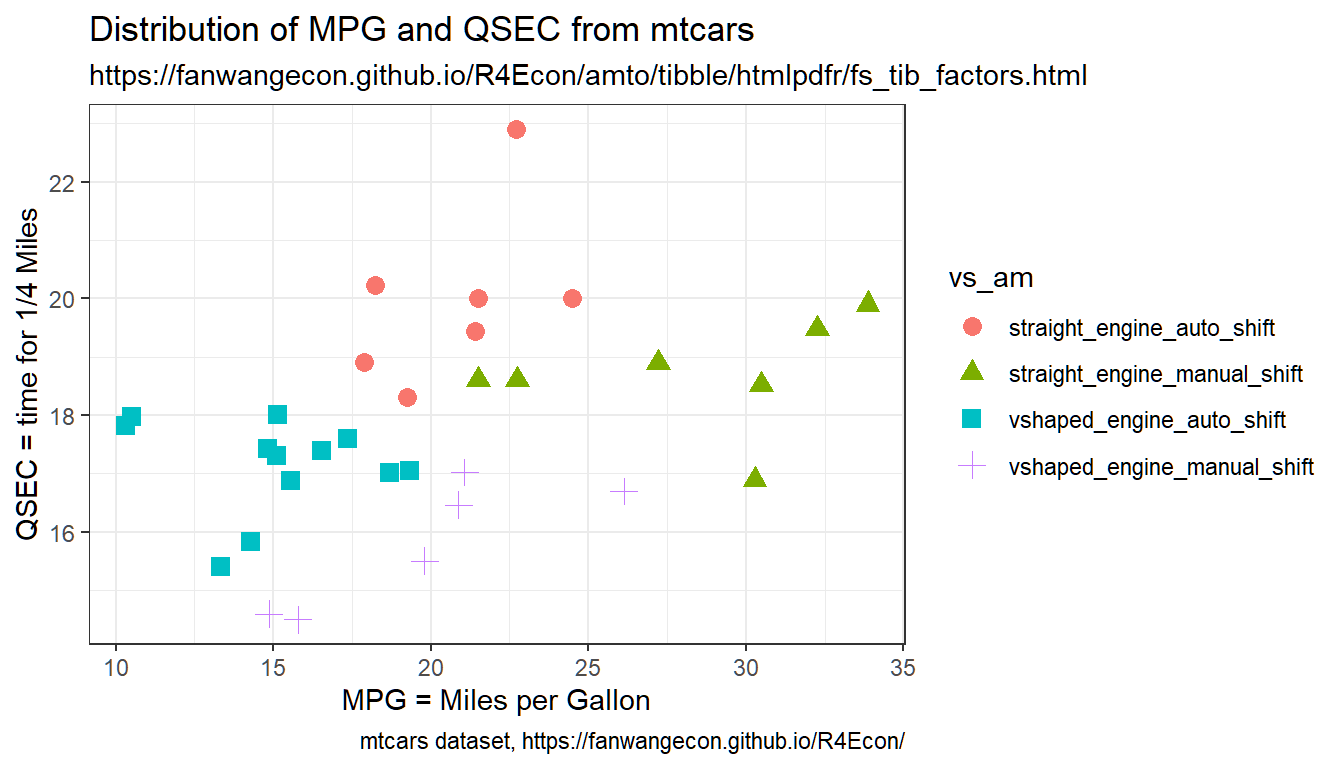
\includegraphics{Panel-Data-and-Optimization-with-R_files/figure-latex/unnamed-chunk-27-1} \end{center}

\hypertarget{draw-random-rows}{%
\subsection{Draw Random Rows}\label{draw-random-rows}}

\begin{quote}
Go back to \href{http://fanwangecon.github.io/}{fan}'s \href{https://fanwangecon.github.io/REconTools/}{REconTools} Package, \href{https://fanwangecon.github.io/R4Econ/}{R4Econ} Repository (\href{https://fanwangecon.github.io/R4Econ/bookdown}{bookdown site}), or \href{https://fanwangecon.github.io/Stat4Econ/}{Intro Stats with R} Repository.
\end{quote}

\hypertarget{draw-random-subset-of-sample}{%
\subsubsection{Draw Random Subset of Sample}\label{draw-random-subset-of-sample}}

\begin{itemize}
\tightlist
\item
  r random discrete
\end{itemize}

We have a sample of N individuals in some dataframe. Draw without replacement a subset \(M<N\) of rows.

\begin{Shaded}
\begin{Highlighting}[]
\CommentTok{# parameters, it_M < it_N}
\NormalTok{it_N <-}\StringTok{ }\DecValTok{10}
\NormalTok{it_M <-}\StringTok{ }\DecValTok{5}

\CommentTok{# Draw it_m from indexed list of it_N}
\KeywordTok{set.seed}\NormalTok{(}\DecValTok{123}\NormalTok{)}
\NormalTok{ar_it_rand_idx <-}\StringTok{ }\KeywordTok{sample}\NormalTok{(it_N, it_M, }\DataTypeTok{replace=}\OtherTok{FALSE}\NormalTok{)}

\CommentTok{# dataframe}
\NormalTok{df_full <-}\StringTok{ }\KeywordTok{as_tibble}\NormalTok{(}\KeywordTok{matrix}\NormalTok{(}\KeywordTok{rnorm}\NormalTok{(}\DecValTok{4}\NormalTok{,}\DataTypeTok{mean=}\DecValTok{0}\NormalTok{,}\DataTypeTok{sd=}\DecValTok{1}\NormalTok{), }\DataTypeTok{nrow=}\NormalTok{it_N, }\DataTypeTok{ncol=}\DecValTok{4}\NormalTok{)) }\OperatorTok\StringTok{ }\KeywordTok{rowid_to_column}\NormalTok{(}\DataTypeTok{var =} \StringTok{"ID"}\NormalTok{)}

\CommentTok{# random Subset}
\NormalTok{df_rand_sub_a <-}\StringTok{ }\NormalTok{df_full[ar_it_rand_idx,]}

\CommentTok{# Random subset also}
\NormalTok{df_rand_sub_b <-}\StringTok{ }\NormalTok{df_full[}\KeywordTok{sample}\NormalTok{(}\KeywordTok{dim}\NormalTok{(df_full)[}\DecValTok{1}\NormalTok{], it_M, }\DataTypeTok{replace=}\OtherTok{FALSE}\NormalTok{),]}

\CommentTok{# Print}
\CommentTok{# Display}
\KeywordTok{kable}\NormalTok{(df_full) }\OperatorTok\StringTok{ }\KeywordTok{kable_styling_fc}\NormalTok{()}
\end{Highlighting}
\end{Shaded}

\begin{table}[!h]
\centering
\begin{tabular}{r|r|r|r|r}
\hline
ID & V1 & V2 & V3 & V4\\
\hline
\rowcolor{gray!6}  1 & 0.1292877 & 0.4609162 & 0.1292877 & 0.4609162\\
\hline
2 & 1.7150650 & -1.2650612 & 1.7150650 & -1.2650612\\
\hline
\rowcolor{gray!6}  3 & 0.4609162 & 0.1292877 & 0.4609162 & 0.1292877\\
\hline
4 & -1.2650612 & 1.7150650 & -1.2650612 & 1.7150650\\
\hline
\rowcolor{gray!6}  5 & 0.1292877 & 0.4609162 & 0.1292877 & 0.4609162\\
\hline
6 & 1.7150650 & -1.2650612 & 1.7150650 & -1.2650612\\
\hline
\rowcolor{gray!6}  7 & 0.4609162 & 0.1292877 & 0.4609162 & 0.1292877\\
\hline
8 & -1.2650612 & 1.7150650 & -1.2650612 & 1.7150650\\
\hline
\rowcolor{gray!6}  9 & 0.1292877 & 0.4609162 & 0.1292877 & 0.4609162\\
\hline
10 & 1.7150650 & -1.2650612 & 1.7150650 & -1.2650612\\
\hline
\end{tabular}
\end{table}

\begin{Shaded}
\begin{Highlighting}[]
\KeywordTok{kable}\NormalTok{(df_rand_sub_a) }\OperatorTok\StringTok{ }\KeywordTok{kable_styling_fc}\NormalTok{()}
\end{Highlighting}
\end{Shaded}

\begin{table}[!h]
\centering
\begin{tabular}{r|r|r|r|r}
\hline
ID & V1 & V2 & V3 & V4\\
\hline
\rowcolor{gray!6}  3 & 0.4609162 & 0.1292877 & 0.4609162 & 0.1292877\\
\hline
10 & 1.7150650 & -1.2650612 & 1.7150650 & -1.2650612\\
\hline
\rowcolor{gray!6}  2 & 1.7150650 & -1.2650612 & 1.7150650 & -1.2650612\\
\hline
8 & -1.2650612 & 1.7150650 & -1.2650612 & 1.7150650\\
\hline
\rowcolor{gray!6}  6 & 1.7150650 & -1.2650612 & 1.7150650 & -1.2650612\\
\hline
\end{tabular}
\end{table}

\begin{Shaded}
\begin{Highlighting}[]
\KeywordTok{kable}\NormalTok{(df_rand_sub_b) }\OperatorTok\StringTok{ }\KeywordTok{kable_styling_fc}\NormalTok{()}
\end{Highlighting}
\end{Shaded}

\begin{table}[!h]
\centering
\begin{tabular}{r|r|r|r|r}
\hline
ID & V1 & V2 & V3 & V4\\
\hline
\rowcolor{gray!6}  5 & 0.1292877 & 0.4609162 & 0.1292877 & 0.4609162\\
\hline
3 & 0.4609162 & 0.1292877 & 0.4609162 & 0.1292877\\
\hline
\rowcolor{gray!6}  9 & 0.1292877 & 0.4609162 & 0.1292877 & 0.4609162\\
\hline
1 & 0.1292877 & 0.4609162 & 0.1292877 & 0.4609162\\
\hline
\rowcolor{gray!6}  4 & -1.2650612 & 1.7150650 & -1.2650612 & 1.7150650\\
\hline
\end{tabular}
\end{table}

\hypertarget{random-subset-of-panel}{%
\subsubsection{Random Subset of Panel}\label{random-subset-of-panel}}

There are \(N\) individuals, each could be observed \(M\) times, but then select a subset of rows only, so each person is randomly observed only a subset of times. Specifically, there there are 3 unique students with student ids, and the second variable shows the random dates in which the student showed up in class, out of the 10 classes available.

\begin{Shaded}
\begin{Highlighting}[]
\CommentTok{# Define}
\NormalTok{it_N <-}\StringTok{ }\DecValTok{3}
\NormalTok{it_M <-}\StringTok{ }\DecValTok{10}
\NormalTok{svr_id <-}\StringTok{ 'student_id'}

\CommentTok{# dataframe}
\KeywordTok{set.seed}\NormalTok{(}\DecValTok{123}\NormalTok{)}
\NormalTok{df_panel_rand <-}\StringTok{ }\KeywordTok{as_tibble}\NormalTok{(}\KeywordTok{matrix}\NormalTok{(it_M, }\DataTypeTok{nrow=}\NormalTok{it_N, }\DataTypeTok{ncol=}\DecValTok{1}\NormalTok{)) }\OperatorTok
\StringTok{  }\KeywordTok{rowid_to_column}\NormalTok{(}\DataTypeTok{var =}\NormalTok{ svr_id) }\OperatorTok
\StringTok{  }\KeywordTok{uncount}\NormalTok{(V1) }\OperatorTok
\StringTok{  }\KeywordTok{group_by}\NormalTok{(}\OperatorTok{!!}\KeywordTok{sym}\NormalTok{(svr_id)) }\OperatorTok\StringTok{ }\KeywordTok{mutate}\NormalTok{(}\DataTypeTok{date =} \KeywordTok{row_number}\NormalTok{()) }\OperatorTok
\StringTok{  }\KeywordTok{ungroup}\NormalTok{() }\OperatorTok\StringTok{ }\KeywordTok{mutate}\NormalTok{(}\DataTypeTok{in_class =} \KeywordTok{case_when}\NormalTok{(}\KeywordTok{rnorm}\NormalTok{(}\KeywordTok{n}\NormalTok{(),}\DataTypeTok{mean=}\DecValTok{0}\NormalTok{,}\DataTypeTok{sd=}\DecValTok{1}\NormalTok{) }\OperatorTok{<}\StringTok{ }\DecValTok{0} \OperatorTok{~}\StringTok{ }\DecValTok{1}\NormalTok{, }\OtherTok{TRUE} \OperatorTok{~}\StringTok{ }\DecValTok{0}\NormalTok{)) }\OperatorTok
\StringTok{  }\KeywordTok{filter}\NormalTok{(in_class }\OperatorTok{==}\StringTok{ }\DecValTok{1}\NormalTok{) }\OperatorTok\StringTok{ }\KeywordTok{select}\NormalTok{(}\OperatorTok{!!}\KeywordTok{sym}\NormalTok{(svr_id), date) }\OperatorTok
\StringTok{  }\KeywordTok{rename}\NormalTok{(}\DataTypeTok{date_in_class =}\NormalTok{ date)}

\CommentTok{# Print}
\KeywordTok{kable}\NormalTok{(df_panel_rand) }\OperatorTok\StringTok{ }\KeywordTok{kable_styling_fc}\NormalTok{()}
\end{Highlighting}
\end{Shaded}

\begin{table}[!h]
\centering
\begin{tabular}{r|r}
\hline
student\_id & date\_in\_class\\
\hline
\rowcolor{gray!6}  1 & 1\\
\hline
1 & 2\\
\hline
\rowcolor{gray!6}  1 & 8\\
\hline
1 & 9\\
\hline
\rowcolor{gray!6}  1 & 10\\
\hline
2 & 5\\
\hline
\rowcolor{gray!6}  2 & 8\\
\hline
2 & 10\\
\hline
\rowcolor{gray!6}  3 & 1\\
\hline
3 & 2\\
\hline
\rowcolor{gray!6}  3 & 3\\
\hline
3 & 4\\
\hline
\rowcolor{gray!6}  3 & 5\\
\hline
3 & 6\\
\hline
\rowcolor{gray!6}  3 & 9\\
\hline
\end{tabular}
\end{table}

\hypertarget{variable-na-values}{%
\subsection{Variable NA Values}\label{variable-na-values}}

\begin{quote}
Go back to \href{http://fanwangecon.github.io/}{fan}'s \href{https://fanwangecon.github.io/REconTools/}{REconTools} Package, \href{https://fanwangecon.github.io/R4Econ/}{R4Econ} Repository (\href{https://fanwangecon.github.io/R4Econ/bookdown}{bookdown site}), or \href{https://fanwangecon.github.io/Stat4Econ/}{Intro Stats with R} Repository.
\end{quote}

\hypertarget{find-and-replace}{%
\subsubsection{Find and Replace}\label{find-and-replace}}

Find and Replace in Dataframe.

\begin{Shaded}
\begin{Highlighting}[]
\CommentTok{# For dataframe}
\NormalTok{df.reg <-df.reg }\OperatorTok\StringTok{ }\KeywordTok{na_if}\NormalTok{(}\OperatorTok{-}\OtherTok{Inf}\NormalTok{) }\OperatorTok\StringTok{ }\KeywordTok{na_if}\NormalTok{(}\OtherTok{Inf}\NormalTok{)}
\CommentTok{# For a specific variable in dataframe}
\NormalTok{df.reg.use }\OperatorTok\StringTok{ }\KeywordTok{mutate}\NormalTok{(}\OperatorTok{!!}\NormalTok{(var.input) }\OperatorTok{:}\ErrorTok{=}\StringTok{ }\KeywordTok{na_if}\NormalTok{(}\OperatorTok{!!}\KeywordTok{sym}\NormalTok{(var.input), }\DecValTok{0}\NormalTok{))}

\CommentTok{# Setting to NA}
\NormalTok{df.reg.use <-}\StringTok{ }\NormalTok{df.reg.guat }\OperatorTok\StringTok{ }\KeywordTok{filter}\NormalTok{(}\OperatorTok{!!}\KeywordTok{sym}\NormalTok{(var.mth) }\OperatorTok{!=}\StringTok{ }\DecValTok{0}\NormalTok{)}
\NormalTok{df.reg.use.log <-}\StringTok{ }\NormalTok{df.reg.use}
\NormalTok{df.reg.use.log[}\KeywordTok{which}\NormalTok{(}\KeywordTok{is.nan}\NormalTok{(df.reg.use}\OperatorTok{$}\NormalTok{prot.imputed.log)),] =}\StringTok{ }\OtherTok{NA}
\NormalTok{df.reg.use.log[}\KeywordTok{which}\NormalTok{(df.reg.use}\OperatorTok{$}\NormalTok{prot.imputed.log}\OperatorTok{==}\OtherTok{Inf}\NormalTok{),] =}\StringTok{ }\OtherTok{NA}
\NormalTok{df.reg.use.log[}\KeywordTok{which}\NormalTok{(df.reg.use}\OperatorTok{$}\NormalTok{prot.imputed.log}\OperatorTok{==-}\OtherTok{Inf}\NormalTok{),] =}\StringTok{ }\OtherTok{NA}
\NormalTok{df.reg.use.log <-}\StringTok{ }\NormalTok{df.reg.use.log }\OperatorTok\StringTok{ }\KeywordTok{drop_na}\NormalTok{(prot.imputed.log)}
\CommentTok{# df.reg.use.log$prot.imputed.log}
\end{Highlighting}
\end{Shaded}

\hypertarget{string-values}{%
\subsection{String Values}\label{string-values}}

\begin{quote}
Go back to \href{http://fanwangecon.github.io/}{fan}'s \href{https://fanwangecon.github.io/REconTools/}{REconTools} Package, \href{https://fanwangecon.github.io/R4Econ/}{R4Econ} Repository (\href{https://fanwangecon.github.io/R4Econ/bookdown}{bookdown site}), or \href{https://fanwangecon.github.io/Stat4Econ/}{Intro Stats with R} Repository.
\end{quote}

\hypertarget{find-and-replace-1}{%
\subsubsection{Find and Replace}\label{find-and-replace-1}}

Find and Replace in Dataframe.

\begin{Shaded}
\begin{Highlighting}[]
\CommentTok{# if string value is contained in variable}
\NormalTok{(}\StringTok{"bridex.B"} \OperatorTok\StringTok{ }\NormalTok{(df.reg.out.all}\OperatorTok{$}\NormalTok{vars_var.y))}
\CommentTok{# if string value is not contained in variable:}
\CommentTok{# 1. type is variable name}
\CommentTok{# 2. Toyota|Mazda are strings to be excluded}
\KeywordTok{filter}\NormalTok{(mtcars, }\OperatorTok{!}\KeywordTok{grepl}\NormalTok{(}\StringTok{'Toyota|Mazda'}\NormalTok{, type))}

\CommentTok{# filter does not contain string}
\NormalTok{rs_hgt_prot_log_tidy }\OperatorTok\StringTok{ }\KeywordTok{filter}\NormalTok{(}\OperatorTok{!}\KeywordTok{str_detect}\NormalTok{(term, }\StringTok{'prot'}\NormalTok{))}
\end{Highlighting}
\end{Shaded}

\hypertarget{summarize-data}{%
\chapter{Summarize Data}\label{summarize-data}}

\hypertarget{counting-observation}{%
\section{Counting Observation}\label{counting-observation}}

\hypertarget{uncount}{%
\subsection{Uncount}\label{uncount}}

\begin{quote}
Go back to \href{http://fanwangecon.github.io/}{fan}'s \href{https://fanwangecon.github.io/REconTools/}{REconTools} Package, \href{https://fanwangecon.github.io/R4Econ/}{R4Econ} Repository (\href{https://fanwangecon.github.io/R4Econ/bookdown}{bookdown site}), or \href{https://fanwangecon.github.io/Stat4Econ/}{Intro Stats with R} Repository.
\end{quote}

In some panel, there are \(N\) individuals, each observed for \(Y_i\) years. Given a dataset with two variables, the individual index, and the \(Y_i\) variable, expand the dataframe so that there is a row for each individual index's each unique year in the survey.

\emph{Search}:

\begin{itemize}
\tightlist
\item
  r duplicate row by variable
\end{itemize}

\emph{Links}:

\begin{itemize}
\tightlist
\item
  see: \href{https://stackoverflow.com/questions/52498169/r-create-duplicate-rows-based-on-a-variable-dplyr-preferred}{Create duplicate rows based on a variable}
\end{itemize}

\emph{Algorithm}:

\begin{enumerate}
\def\labelenumi{\arabic{enumi}.}
\tightlist
\item
  generate testing frame, the individual attribute dataset with invariant information over panel
\item
  uncount, duplicate rows by years in survey
\item
  group and generate sorted index
\item
  add indiviual specific stat year to index
\end{enumerate}

\begin{Shaded}
\begin{Highlighting}[]
\CommentTok{# 1. Array of Years in the Survey}
\NormalTok{ar_years_in_survey <-}\StringTok{ }\KeywordTok{c}\NormalTok{(}\DecValTok{2}\NormalTok{,}\DecValTok{3}\NormalTok{,}\DecValTok{1}\NormalTok{,}\DecValTok{10}\NormalTok{,}\DecValTok{2}\NormalTok{,}\DecValTok{5}\NormalTok{)}
\NormalTok{ar_start_yaer <-}\StringTok{ }\KeywordTok{c}\NormalTok{(}\DecValTok{1}\NormalTok{,}\DecValTok{2}\NormalTok{,}\DecValTok{3}\NormalTok{,}\DecValTok{1}\NormalTok{,}\DecValTok{1}\NormalTok{,}\DecValTok{1}\NormalTok{)}
\NormalTok{ar_end_year <-}\StringTok{ }\KeywordTok{c}\NormalTok{(}\DecValTok{2}\NormalTok{,}\DecValTok{4}\NormalTok{,}\DecValTok{3}\NormalTok{,}\DecValTok{10}\NormalTok{,}\DecValTok{2}\NormalTok{,}\DecValTok{5}\NormalTok{)}
\NormalTok{mt_combine <-}\StringTok{ }\KeywordTok{cbind}\NormalTok{(ar_years_in_survey, ar_start_yaer, ar_end_year)}

\CommentTok{# This is the individual attribute dataset, attributes that are invariant acrosss years}
\NormalTok{tb_indi_attributes <-}\StringTok{ }\KeywordTok{as_tibble}\NormalTok{(mt_combine) }\OperatorTok\StringTok{ }\KeywordTok{rowid_to_column}\NormalTok{(}\DataTypeTok{var =} \StringTok{"ID"}\NormalTok{)}

\CommentTok{# 2. Sort and generate variable equal to sorted index}
\NormalTok{tb_indi_panel <-}\StringTok{ }\NormalTok{tb_indi_attributes }\OperatorTok\StringTok{ }\KeywordTok{uncount}\NormalTok{(ar_years_in_survey)}

\CommentTok{# 3. Panel now construct exactly which year in survey, note that all needed is sort index}
\CommentTok{# Note sorting not needed, all rows identical now}
\NormalTok{tb_indi_panel <-}\StringTok{ }\NormalTok{tb_indi_panel }\OperatorTok
\StringTok{                    }\KeywordTok{group_by}\NormalTok{(ID) }\OperatorTok
\StringTok{                    }\KeywordTok{mutate}\NormalTok{(}\DataTypeTok{yr_in_survey =} \KeywordTok{row_number}\NormalTok{())}

\NormalTok{tb_indi_panel <-}\StringTok{ }\NormalTok{tb_indi_panel }\OperatorTok
\StringTok{                    }\KeywordTok{mutate}\NormalTok{(}\DataTypeTok{calendar_year =}\NormalTok{ yr_in_survey }\OperatorTok{+}\StringTok{ }\NormalTok{ar_start_yaer }\OperatorTok{-}\StringTok{ }\DecValTok{1}\NormalTok{)}

\CommentTok{# Show results Head 10}
\NormalTok{tb_indi_panel }\OperatorTok\StringTok{ }\KeywordTok{head}\NormalTok{(}\DecValTok{10}\NormalTok{) }\OperatorTok
\StringTok{  }\KeywordTok{kable}\NormalTok{() }\OperatorTok
\StringTok{  }\KeywordTok{kable_styling_fc}\NormalTok{()}
\end{Highlighting}
\end{Shaded}

\begin{table}[!h]
\centering
\begin{tabular}{r|r|r|r|r}
\hline
ID & ar\_start\_yaer & ar\_end\_year & yr\_in\_survey & calendar\_year\\
\hline
\rowcolor{gray!6}  1 & 1 & 2 & 1 & 1\\
\hline
1 & 1 & 2 & 2 & 2\\
\hline
\rowcolor{gray!6}  2 & 2 & 4 & 1 & 2\\
\hline
2 & 2 & 4 & 2 & 3\\
\hline
\rowcolor{gray!6}  2 & 2 & 4 & 3 & 4\\
\hline
3 & 3 & 3 & 1 & 3\\
\hline
\rowcolor{gray!6}  4 & 1 & 10 & 1 & 1\\
\hline
4 & 1 & 10 & 2 & 2\\
\hline
\rowcolor{gray!6}  4 & 1 & 10 & 3 & 3\\
\hline
4 & 1 & 10 & 4 & 4\\
\hline
\end{tabular}
\end{table}

\hypertarget{sorting-indexing-slicing}{%
\section{Sorting, Indexing, Slicing}\label{sorting-indexing-slicing}}

\hypertarget{sorting}{%
\subsection{Sorting}\label{sorting}}

\begin{quote}
Go back to \href{http://fanwangecon.github.io/}{fan}'s \href{https://fanwangecon.github.io/REconTools/}{REconTools} Package, \href{https://fanwangecon.github.io/R4Econ/}{R4Econ} Repository (\href{https://fanwangecon.github.io/R4Econ/bookdown}{bookdown site}), or \href{https://fanwangecon.github.io/Stat4Econ/}{Intro Stats with R} Repository.
\end{quote}

\hypertarget{generate-sorted-index-within-group-with-repeating-values}{%
\subsubsection{Generate Sorted Index within Group with Repeating Values}\label{generate-sorted-index-within-group-with-repeating-values}}

There is a variable, sort by this variable, then generate index from 1 to N representing sorted values of this index. If there are repeating values, still assign index, different index each value.

\begin{itemize}
\tightlist
\item
  r generate index sort
\item
  dplyr mutate equals index
\end{itemize}

\begin{Shaded}
\begin{Highlighting}[]
\CommentTok{# Sort and generate variable equal to sorted index}
\NormalTok{df_iris <-}\StringTok{ }\NormalTok{iris }\OperatorTok\StringTok{ }\KeywordTok{arrange}\NormalTok{(Sepal.Length) }\OperatorTok
\StringTok{              }\KeywordTok{mutate}\NormalTok{(}\DataTypeTok{Sepal.Len.Index =} \KeywordTok{row_number}\NormalTok{()) }\OperatorTok
\StringTok{              }\KeywordTok{select}\NormalTok{(Sepal.Length, Sepal.Len.Index, }\KeywordTok{everything}\NormalTok{())}

\CommentTok{# Show results Head 10}
\NormalTok{df_iris }\OperatorTok\StringTok{ }\KeywordTok{head}\NormalTok{(}\DecValTok{10}\NormalTok{) }\OperatorTok
\StringTok{  }\KeywordTok{kable}\NormalTok{() }\OperatorTok
\StringTok{  }\KeywordTok{kable_styling_fc_wide}\NormalTok{()}
\end{Highlighting}
\end{Shaded}

\begin{table}[!h]
\centering
\resizebox{\linewidth}{!}{
\begin{tabular}{r|r|r|r|r|l}
\hline
Sepal.Length & Sepal.Len.Index & Sepal.Width & Petal.Length & Petal.Width & Species\\
\hline
\rowcolor{gray!6}  4.3 & 1 & 3.0 & 1.1 & 0.1 & setosa\\
\hline
4.4 & 2 & 2.9 & 1.4 & 0.2 & setosa\\
\hline
\rowcolor{gray!6}  4.4 & 3 & 3.0 & 1.3 & 0.2 & setosa\\
\hline
4.4 & 4 & 3.2 & 1.3 & 0.2 & setosa\\
\hline
\rowcolor{gray!6}  4.5 & 5 & 2.3 & 1.3 & 0.3 & setosa\\
\hline
4.6 & 6 & 3.1 & 1.5 & 0.2 & setosa\\
\hline
\rowcolor{gray!6}  4.6 & 7 & 3.4 & 1.4 & 0.3 & setosa\\
\hline
4.6 & 8 & 3.6 & 1.0 & 0.2 & setosa\\
\hline
\rowcolor{gray!6}  4.6 & 9 & 3.2 & 1.4 & 0.2 & setosa\\
\hline
4.7 & 10 & 3.2 & 1.3 & 0.2 & setosa\\
\hline
\end{tabular}}
\end{table}

\hypertarget{populate-value-from-lowest-index-to-all-other-rows}{%
\subsubsection{Populate Value from Lowest Index to All other Rows}\label{populate-value-from-lowest-index-to-all-other-rows}}

We would like to calculate for example the ratio of each individual's highest to the the person with the lowest height in a dataset. We first need to generated sorted index from lowest to highest, and then populate the lowest height to all rows, and then divide.

\emph{Search Terms}:

\begin{itemize}
\tightlist
\item
  r spread value to all rows from one row
\item
  r other rows equal to the value of one row
\item
  Conditional assignment of one variable to the value of one of two other variables
\item
  dplyr mutate conditional
\item
  dplyr value from one row to all rows
\item
  dplyr mutate equal to value in another cell
\end{itemize}

\emph{Links}:

\begin{itemize}
\tightlist
\item
  see: dplyr \href{https://dplyr.tidyverse.org/reference/ranking.html}{rank}
\item
  see: dplyr \href{https://dplyr.tidyverse.org/reference/case_when.html}{case\_when}
\end{itemize}

\hypertarget{short-method-mutate-and-min}{%
\paragraph{Short Method: mutate and min}\label{short-method-mutate-and-min}}

We just want the lowest value to be in its own column, so that we can compute various statistics using the lowest value variable and the original variable.

\begin{Shaded}
\begin{Highlighting}[]
\CommentTok{# 1. Sort}
\NormalTok{df_iris_m1 <-}\StringTok{ }\NormalTok{iris }\OperatorTok\StringTok{ }\KeywordTok{mutate}\NormalTok{(}\DataTypeTok{Sepal.Len.Lowest.all =} \KeywordTok{min}\NormalTok{(Sepal.Length)) }\OperatorTok
\StringTok{                }\KeywordTok{select}\NormalTok{(Sepal.Length, Sepal.Len.Lowest.all, }\KeywordTok{everything}\NormalTok{())}


\CommentTok{# Show results Head 10}
\NormalTok{df_iris_m1 }\OperatorTok\StringTok{ }\KeywordTok{head}\NormalTok{(}\DecValTok{10}\NormalTok{) }\OperatorTok
\StringTok{  }\KeywordTok{kable}\NormalTok{() }\OperatorTok
\StringTok{  }\KeywordTok{kable_styling_fc_wide}\NormalTok{()}
\end{Highlighting}
\end{Shaded}

\begin{table}[!h]
\centering
\resizebox{\linewidth}{!}{
\begin{tabular}{r|r|r|r|r|l}
\hline
Sepal.Length & Sepal.Len.Lowest.all & Sepal.Width & Petal.Length & Petal.Width & Species\\
\hline
\rowcolor{gray!6}  5.1 & 4.3 & 3.5 & 1.4 & 0.2 & setosa\\
\hline
4.9 & 4.3 & 3.0 & 1.4 & 0.2 & setosa\\
\hline
\rowcolor{gray!6}  4.7 & 4.3 & 3.2 & 1.3 & 0.2 & setosa\\
\hline
4.6 & 4.3 & 3.1 & 1.5 & 0.2 & setosa\\
\hline
\rowcolor{gray!6}  5.0 & 4.3 & 3.6 & 1.4 & 0.2 & setosa\\
\hline
5.4 & 4.3 & 3.9 & 1.7 & 0.4 & setosa\\
\hline
\rowcolor{gray!6}  4.6 & 4.3 & 3.4 & 1.4 & 0.3 & setosa\\
\hline
5.0 & 4.3 & 3.4 & 1.5 & 0.2 & setosa\\
\hline
\rowcolor{gray!6}  4.4 & 4.3 & 2.9 & 1.4 & 0.2 & setosa\\
\hline
4.9 & 4.3 & 3.1 & 1.5 & 0.1 & setosa\\
\hline
\end{tabular}}
\end{table}

\hypertarget{long-method-row_number-and-case_when}{%
\paragraph{Long Method: row\_number and case\_when}\label{long-method-row_number-and-case_when}}

This is the long method, using row\_number, and case\_when. The benefit of this method is that it generates several intermediate variables that might be useful. And the key final step is to set a new variable (A=\emph{Sepal.Len.Lowest.all}) equal to another variable's (B=\emph{Sepal.Length}'s) value at the index that satisfies condition based a third variable (C=\emph{Sepal.Len.Index}).

\begin{Shaded}
\begin{Highlighting}[]
\CommentTok{# 1. Sort}
\CommentTok{# 2. generate index}
\CommentTok{# 3. value at lowest index (case_when)}
\CommentTok{# 4. spread value from lowest index to other rows}
\CommentTok{# Note step 4 does not require step 3}
\NormalTok{df_iris_m2 <-}\StringTok{ }\NormalTok{iris }\OperatorTok\StringTok{ }\KeywordTok{arrange}\NormalTok{(Sepal.Length) }\OperatorTok
\StringTok{              }\KeywordTok{mutate}\NormalTok{(}\DataTypeTok{Sepal.Len.Index =} \KeywordTok{row_number}\NormalTok{()) }\OperatorTok
\StringTok{              }\KeywordTok{mutate}\NormalTok{(}\DataTypeTok{Sepal.Len.Lowest.one =}
                       \KeywordTok{case_when}\NormalTok{(}\KeywordTok{row_number}\NormalTok{()}\OperatorTok{==}\DecValTok{1} \OperatorTok{~}\StringTok{ }\NormalTok{Sepal.Length)) }\OperatorTok
\StringTok{              }\KeywordTok{mutate}\NormalTok{(}\DataTypeTok{Sepal.Len.Lowest.all =}
\NormalTok{                       Sepal.Length[Sepal.Len.Index}\OperatorTok{==}\DecValTok{1}\NormalTok{]) }\OperatorTok
\StringTok{              }\KeywordTok{select}\NormalTok{(Sepal.Length, Sepal.Len.Index,}
\NormalTok{                     Sepal.Len.Lowest.one, Sepal.Len.Lowest.all)}


\CommentTok{# Show results Head 10}
\NormalTok{df_iris_m2 }\OperatorTok\StringTok{ }\KeywordTok{head}\NormalTok{(}\DecValTok{10}\NormalTok{) }\OperatorTok
\StringTok{  }\KeywordTok{kable}\NormalTok{() }\OperatorTok
\StringTok{  }\KeywordTok{kable_styling_fc_wide}\NormalTok{()}
\end{Highlighting}
\end{Shaded}

\begin{table}[!h]
\centering
\resizebox{\linewidth}{!}{
\begin{tabular}{r|r|r|r}
\hline
Sepal.Length & Sepal.Len.Index & Sepal.Len.Lowest.one & Sepal.Len.Lowest.all\\
\hline
\rowcolor{gray!6}  4.3 & 1 & 4.3 & 4.3\\
\hline
4.4 & 2 & NA & 4.3\\
\hline
\rowcolor{gray!6}  4.4 & 3 & NA & 4.3\\
\hline
4.4 & 4 & NA & 4.3\\
\hline
\rowcolor{gray!6}  4.5 & 5 & NA & 4.3\\
\hline
4.6 & 6 & NA & 4.3\\
\hline
\rowcolor{gray!6}  4.6 & 7 & NA & 4.3\\
\hline
4.6 & 8 & NA & 4.3\\
\hline
\rowcolor{gray!6}  4.6 & 9 & NA & 4.3\\
\hline
4.7 & 10 & NA & 4.3\\
\hline
\end{tabular}}
\end{table}

\hypertarget{generate-sorted-index-based-on-deviations}{%
\subsubsection{Generate Sorted Index based on Deviations}\label{generate-sorted-index-based-on-deviations}}

Generate Positive and Negative Index based on Ordered Deviation from some Number.

There is a variable that is continuous, substract a number from this variable, and generate index based on deviations. Think of the index as generating intervals indicating where the value lies. 0th index indicates the largest value in sequence that is smaller than or equal to number \(x\), 1st index indicates the smallest value in sequence that is larger than number \(x\).

The solution below is a little bit convoluated and long, there is likely a much quicker way. The process below shows various intermediary outputs that help arrive at deviation index \emph{Sepal.Len.Devi.Index} from initial sorted index \emph{Sepal.Len.Index}.

\emph{search}:

\begin{itemize}
\tightlist
\item
  dplyr arrange ignore na
\item
  dplyr index deviation from order number sequence
\item
  dplyr index below above
\item
  dplyr index order below above value
\end{itemize}

\begin{Shaded}
\begin{Highlighting}[]
\CommentTok{# 1. Sort and generate variable equal to sorted index}
\CommentTok{# 2. Plus or minus deviations from some value}
\CommentTok{# 3. Find the zero, which means, the number closests to zero including zero from the negative side}
\CommentTok{# 4. Find the index at the highest zero and below deviation point}
\CommentTok{# 5. Difference of zero index and original sorted index}
\NormalTok{sc_val_x <-}\StringTok{ }\FloatTok{4.65}
\NormalTok{df_iris_deviate <-}\StringTok{ }\NormalTok{iris }\OperatorTok\StringTok{ }\KeywordTok{arrange}\NormalTok{(Sepal.Length) }\OperatorTok
\StringTok{              }\KeywordTok{mutate}\NormalTok{(}\DataTypeTok{Sepal.Len.Index =} \KeywordTok{row_number}\NormalTok{()) }\OperatorTok
\StringTok{              }\KeywordTok{mutate}\NormalTok{(}\DataTypeTok{Sepal.Len.Devi =}\NormalTok{ (Sepal.Length }\OperatorTok{-}\StringTok{ }\NormalTok{sc_val_x)) }\OperatorTok
\StringTok{              }\KeywordTok{mutate}\NormalTok{(}\DataTypeTok{Sepal.Len.Devi.Neg =}
                       \KeywordTok{case_when}\NormalTok{(Sepal.Len.Devi }\OperatorTok{<=}\StringTok{ }\DecValTok{0} \OperatorTok{~}\StringTok{ }\NormalTok{(}\OperatorTok{-}\DecValTok{1}\NormalTok{)}\OperatorTok{*}\NormalTok{(Sepal.Len.Devi))) }\OperatorTok
\StringTok{              }\KeywordTok{arrange}\NormalTok{((Sepal.Len.Devi.Neg), }\KeywordTok{desc}\NormalTok{(Sepal.Len.Index)) }\OperatorTok
\StringTok{              }\KeywordTok{mutate}\NormalTok{(}\DataTypeTok{Sepal.Len.Index.Zero =}
                       \KeywordTok{case_when}\NormalTok{(}\KeywordTok{row_number}\NormalTok{() }\OperatorTok{==}\StringTok{ }\DecValTok{1} \OperatorTok{~}\StringTok{ }\NormalTok{Sepal.Len.Index)) }\OperatorTok
\StringTok{              }\KeywordTok{mutate}\NormalTok{(}\DataTypeTok{Sepal.Len.Devi.Index =}
\NormalTok{                       Sepal.Len.Index }\OperatorTok{-}\StringTok{ }\NormalTok{Sepal.Len.Index.Zero[}\KeywordTok{row_number}\NormalTok{() }\OperatorTok{==}\StringTok{ }\DecValTok{1}\NormalTok{]) }\OperatorTok
\StringTok{              }\KeywordTok{arrange}\NormalTok{(Sepal.Len.Index) }\OperatorTok
\StringTok{              }\KeywordTok{select}\NormalTok{(Sepal.Length, Sepal.Len.Index, Sepal.Len.Devi,}
\NormalTok{                     Sepal.Len.Devi.Neg, Sepal.Len.Index.Zero, Sepal.Len.Devi.Index)}


\CommentTok{# Show results Head 10}
\NormalTok{df_iris_deviate }\OperatorTok\StringTok{ }\KeywordTok{head}\NormalTok{(}\DecValTok{20}\NormalTok{) }\OperatorTok
\StringTok{  }\KeywordTok{kable}\NormalTok{() }\OperatorTok
\StringTok{  }\KeywordTok{kable_styling_fc_wide}\NormalTok{()}
\end{Highlighting}
\end{Shaded}

\begin{table}[!h]
\centering
\resizebox{\linewidth}{!}{
\begin{tabular}{r|r|r|r|r|r}
\hline
Sepal.Length & Sepal.Len.Index & Sepal.Len.Devi & Sepal.Len.Devi.Neg & Sepal.Len.Index.Zero & Sepal.Len.Devi.Index\\
\hline
\rowcolor{gray!6}  4.3 & 1 & -0.35 & 0.35 & NA & -8\\
\hline
4.4 & 2 & -0.25 & 0.25 & NA & -7\\
\hline
\rowcolor{gray!6}  4.4 & 3 & -0.25 & 0.25 & NA & -6\\
\hline
4.4 & 4 & -0.25 & 0.25 & NA & -5\\
\hline
\rowcolor{gray!6}  4.5 & 5 & -0.15 & 0.15 & NA & -4\\
\hline
4.6 & 6 & -0.05 & 0.05 & NA & -3\\
\hline
\rowcolor{gray!6}  4.6 & 7 & -0.05 & 0.05 & NA & -2\\
\hline
4.6 & 8 & -0.05 & 0.05 & NA & -1\\
\hline
\rowcolor{gray!6}  4.6 & 9 & -0.05 & 0.05 & 9 & 0\\
\hline
4.7 & 10 & 0.05 & NA & NA & 1\\
\hline
\rowcolor{gray!6}  4.7 & 11 & 0.05 & NA & NA & 2\\
\hline
4.8 & 12 & 0.15 & NA & NA & 3\\
\hline
\rowcolor{gray!6}  4.8 & 13 & 0.15 & NA & NA & 4\\
\hline
4.8 & 14 & 0.15 & NA & NA & 5\\
\hline
\rowcolor{gray!6}  4.8 & 15 & 0.15 & NA & NA & 6\\
\hline
4.8 & 16 & 0.15 & NA & NA & 7\\
\hline
\rowcolor{gray!6}  4.9 & 17 & 0.25 & NA & NA & 8\\
\hline
4.9 & 18 & 0.25 & NA & NA & 9\\
\hline
\rowcolor{gray!6}  4.9 & 19 & 0.25 & NA & NA & 10\\
\hline
4.9 & 20 & 0.25 & NA & NA & 11\\
\hline
\end{tabular}}
\end{table}

\hypertarget{group-statistics}{%
\section{Group Statistics}\label{group-statistics}}

\hypertarget{groups-statistics}{%
\subsection{Groups Statistics}\label{groups-statistics}}

\begin{quote}
Go back to \href{http://fanwangecon.github.io/}{fan}'s \href{https://fanwangecon.github.io/REconTools/}{REconTools} Package, \href{https://fanwangecon.github.io/R4Econ/}{R4Econ} Repository (\href{https://fanwangecon.github.io/R4Econ/bookdown}{bookdown site}), or \href{https://fanwangecon.github.io/Stat4Econ/}{Intro Stats with R} Repository.
\end{quote}

\hypertarget{aggrgate-groups-only-unique-group-and-count}{%
\subsubsection{Aggrgate Groups only Unique Group and Count}\label{aggrgate-groups-only-unique-group-and-count}}

There are two variables that are numeric, we want to find all the unique groups of these two variables in a dataset and count how many times each unique group occurs

\begin{itemize}
\tightlist
\item
  r unique occurrence of numeric groups
\item
  How to add count of unique values by group to R data.frame
\end{itemize}

\begin{Shaded}
\begin{Highlighting}[]
\CommentTok{# Numeric value combinations unique Groups}
\NormalTok{vars.group <-}\StringTok{ }\KeywordTok{c}\NormalTok{(}\StringTok{'hgt0'}\NormalTok{, }\StringTok{'wgt0'}\NormalTok{)}

\CommentTok{# dataset subsetting}
\NormalTok{df_use <-}\StringTok{ }\NormalTok{df_hgt_wgt }\OperatorTok\StringTok{ }\KeywordTok{select}\NormalTok{(}\OperatorTok{!!!}\KeywordTok{syms}\NormalTok{(}\KeywordTok{c}\NormalTok{(vars.group))) }\OperatorTok
\StringTok{            }\KeywordTok{mutate}\NormalTok{(}\DataTypeTok{hgt0 =} \KeywordTok{round}\NormalTok{(hgt0}\OperatorTok{/}\DecValTok{5}\NormalTok{)}\OperatorTok{*}\DecValTok{5}\NormalTok{, }\DataTypeTok{wgt0 =} \KeywordTok{round}\NormalTok{(wgt0}\OperatorTok{/}\DecValTok{2000}\NormalTok{)}\OperatorTok{*}\DecValTok{2000}\NormalTok{) }\OperatorTok
\StringTok{            }\KeywordTok{drop_na}\NormalTok{()}

\CommentTok{# Group, count and generate means for each numeric variables}
\CommentTok{# mutate_at(vars.group, funs(as.factor(.))) %>%}
\NormalTok{df.group.count <-}\StringTok{ }\NormalTok{df_use }\OperatorTok\StringTok{ }\KeywordTok{group_by}\NormalTok{(}\OperatorTok{!!!}\KeywordTok{syms}\NormalTok{(vars.group)) }\OperatorTok
\StringTok{                    }\KeywordTok{arrange}\NormalTok{(}\OperatorTok{!!!}\KeywordTok{syms}\NormalTok{(vars.group)) }\OperatorTok
\StringTok{                    }\KeywordTok{summarise}\NormalTok{(}\DataTypeTok{n_obs_group=}\KeywordTok{n}\NormalTok{())}

\CommentTok{# Show results Head 10}
\NormalTok{df.group.count }\OperatorTok\StringTok{ }\KeywordTok{kable}\NormalTok{() }\OperatorTok\StringTok{ }\KeywordTok{kable_styling_fc}\NormalTok{()}
\end{Highlighting}
\end{Shaded}

\begin{table}[!h]
\centering
\begin{tabular}{r|r|r}
\hline
hgt0 & wgt0 & n\_obs\_group\\
\hline
\rowcolor{gray!6}  40 & 2000 & 122\\
\hline
45 & 2000 & 4586\\
\hline
\rowcolor{gray!6}  45 & 4000 & 470\\
\hline
50 & 2000 & 9691\\
\hline
\rowcolor{gray!6}  50 & 4000 & 13106\\
\hline
55 & 2000 & 126\\
\hline
\rowcolor{gray!6}  55 & 4000 & 1900\\
\hline
60 & 6000 & 18\\
\hline
\end{tabular}
\end{table}

\hypertarget{aggrgate-groups-only-unique-group-show-up-with-means}{%
\subsubsection{Aggrgate Groups only Unique Group Show up With Means}\label{aggrgate-groups-only-unique-group-show-up-with-means}}

Several variables that are grouping identifiers. Several variables that are values which mean be unique for each group members. For example, a Panel of income for N households over T years with also household education information that is invariant over time. Want to generate a dataset where the unit of observation are households, rather than household years. Take average of all numeric variables that are household and year specific.

A complicating factor potentially is that the number of observations differ within group, for example, income might be observed for all years for some households but not for other households.

\begin{itemize}
\tightlist
\item
  r dplyr aggregate group average
\item
  Aggregating and analyzing data with dplyr
\item
  column can't be modified because it is a grouping variable
\item
  see also: \href{https://datacarpentry.org/dc_zurich/R-ecology/04-dplyr.html}{Aggregating and analyzing data with dplyr}
\end{itemize}

\begin{Shaded}
\begin{Highlighting}[]
\CommentTok{# In the df_hgt_wgt from R4Econ, there is a country id, village id,}
\CommentTok{# and individual id, and various other statistics}
\NormalTok{vars.group <-}\StringTok{ }\KeywordTok{c}\NormalTok{(}\StringTok{'S.country'}\NormalTok{, }\StringTok{'vil.id'}\NormalTok{, }\StringTok{'indi.id'}\NormalTok{)}
\NormalTok{vars.values <-}\StringTok{ }\KeywordTok{c}\NormalTok{(}\StringTok{'hgt'}\NormalTok{, }\StringTok{'momEdu'}\NormalTok{)}

\CommentTok{# dataset subsetting}
\NormalTok{df_use <-}\StringTok{ }\NormalTok{df_hgt_wgt }\OperatorTok\StringTok{ }\KeywordTok{select}\NormalTok{(}\OperatorTok{!!!}\KeywordTok{syms}\NormalTok{(}\KeywordTok{c}\NormalTok{(vars.group, vars.values)))}

\CommentTok{# Group, count and generate means for each numeric variables}
\NormalTok{df.group <-}\StringTok{ }\NormalTok{df_use }\OperatorTok\StringTok{ }\KeywordTok{group_by}\NormalTok{(}\OperatorTok{!!!}\KeywordTok{syms}\NormalTok{(vars.group)) }\OperatorTok
\StringTok{            }\KeywordTok{arrange}\NormalTok{(}\OperatorTok{!!!}\KeywordTok{syms}\NormalTok{(vars.group)) }\OperatorTok
\StringTok{            }\KeywordTok{summarise_if}\NormalTok{(is.numeric,}
                         \KeywordTok{funs}\NormalTok{(}\DataTypeTok{mean =} \KeywordTok{mean}\NormalTok{(., }\DataTypeTok{na.rm =} \OtherTok{TRUE}\NormalTok{),}
                              \DataTypeTok{sd =} \KeywordTok{sd}\NormalTok{(., }\DataTypeTok{na.rm =} \OtherTok{TRUE}\NormalTok{),}
                              \DataTypeTok{n =} \KeywordTok{sum}\NormalTok{(}\KeywordTok{is.na}\NormalTok{(.)}\OperatorTok{==}\DecValTok{0}\NormalTok{)))}

\CommentTok{# Show results Head 10}
\NormalTok{df.group }\OperatorTok\StringTok{ }\KeywordTok{head}\NormalTok{(}\DecValTok{10}\NormalTok{) }\OperatorTok
\StringTok{  }\KeywordTok{kable}\NormalTok{() }\OperatorTok
\StringTok{  }\KeywordTok{kable_styling_fc_wide}\NormalTok{()}
\end{Highlighting}
\end{Shaded}

\begin{table}[!h]
\centering
\resizebox{\linewidth}{!}{
\begin{tabular}{l|r|r|r|r|r|r|r|r}
\hline
S.country & vil.id & indi.id & hgt\_mean & momEdu\_mean & hgt\_sd & momEdu\_sd & hgt\_n & momEdu\_n\\
\hline
\rowcolor{gray!6}  Cebu & 1 & 1 & 61.80000 & 5.3 & 9.520504 & 0 & 7 & 18\\
\hline
Cebu & 1 & 2 & 68.86154 & 7.1 & 9.058931 & 0 & 13 & 18\\
\hline
\rowcolor{gray!6}  Cebu & 1 & 3 & 80.45882 & 9.4 & 29.894231 & 0 & 17 & 18\\
\hline
Cebu & 1 & 4 & 88.10000 & 13.9 & 35.533166 & 0 & 18 & 18\\
\hline
\rowcolor{gray!6}  Cebu & 1 & 5 & 97.70556 & 11.3 & 41.090366 & 0 & 18 & 18\\
\hline
Cebu & 1 & 6 & 87.49444 & 7.3 & 35.586439 & 0 & 18 & 18\\
\hline
\rowcolor{gray!6}  Cebu & 1 & 7 & 90.79412 & 10.4 & 38.722385 & 0 & 17 & 18\\
\hline
Cebu & 1 & 8 & 68.45385 & 13.5 & 10.011961 & 0 & 13 & 18\\
\hline
\rowcolor{gray!6}  Cebu & 1 & 9 & 86.21111 & 10.4 & 35.126057 & 0 & 18 & 18\\
\hline
Cebu & 1 & 10 & 87.67222 & 10.5 & 36.508127 & 0 & 18 & 18\\
\hline
\end{tabular}}
\end{table}

\begin{Shaded}
\begin{Highlighting}[]
\CommentTok{# Show results Head 10}
\NormalTok{df.group }\OperatorTok\StringTok{ }\KeywordTok{tail}\NormalTok{(}\DecValTok{10}\NormalTok{) }\OperatorTok
\StringTok{  }\KeywordTok{kable}\NormalTok{() }\OperatorTok
\StringTok{  }\KeywordTok{kable_styling_fc_wide}\NormalTok{()}
\end{Highlighting}
\end{Shaded}

\begin{table}[!h]
\centering
\resizebox{\linewidth}{!}{
\begin{tabular}{l|r|r|r|r|r|r|r|r}
\hline
S.country & vil.id & indi.id & hgt\_mean & momEdu\_mean & hgt\_sd & momEdu\_sd & hgt\_n & momEdu\_n\\
\hline
\rowcolor{gray!6}  Guatemala & 14 & 2014 & 66.97000 & NaN & 8.967974 & NaN & 10 & 0\\
\hline
Guatemala & 14 & 2015 & 71.71818 & NaN & 11.399984 & NaN & 11 & 0\\
\hline
\rowcolor{gray!6}  Guatemala & 14 & 2016 & 66.33000 & NaN & 9.490352 & NaN & 10 & 0\\
\hline
Guatemala & 14 & 2017 & 76.40769 & NaN & 14.827871 & NaN & 13 & 0\\
\hline
\rowcolor{gray!6}  Guatemala & 14 & 2018 & 74.55385 & NaN & 12.707846 & NaN & 13 & 0\\
\hline
Guatemala & 14 & 2019 & 70.47500 & NaN & 11.797390 & NaN & 12 & 0\\
\hline
\rowcolor{gray!6}  Guatemala & 14 & 2020 & 60.28750 & NaN & 7.060036 & NaN & 8 & 0\\
\hline
Guatemala & 14 & 2021 & 84.96000 & NaN & 15.446193 & NaN & 10 & 0\\
\hline
\rowcolor{gray!6}  Guatemala & 14 & 2022 & 79.38667 & NaN & 15.824749 & NaN & 15 & 0\\
\hline
Guatemala & 14 & 2023 & 66.50000 & NaN & 8.613113 & NaN & 8 & 0\\
\hline
\end{tabular}}
\end{table}

\hypertarget{one-variable-group-summary}{%
\subsection{One Variable Group Summary}\label{one-variable-group-summary}}

\begin{quote}
Go back to \href{http://fanwangecon.github.io/}{fan}'s \href{https://fanwangecon.github.io/REconTools/}{REconTools} Package, \href{https://fanwangecon.github.io/R4Econ/}{R4Econ} Repository (\href{https://fanwangecon.github.io/R4Econ/bookdown}{bookdown site}), or \href{https://fanwangecon.github.io/Stat4Econ/}{Intro Stats with R} Repository.
\end{quote}

There is a categorical variable (based on one or the interaction of multiple variables), there is a continuous variable, obtain statistics for the continuous variable conditional on the categorical variable, but also unconditionally.

Store results in a matrix, but also flatten results wide to row with appropriate keys/variable-names for all group statistics.

Pick which statistics to be included in final wide row

\hypertarget{build-program}{%
\subsubsection{Build Program}\label{build-program}}

\begin{Shaded}
\begin{Highlighting}[]
\CommentTok{# Single Variable Group Statistics (also generate overall statistics)}
\NormalTok{ff_summ_by_group_summ_one <-}\StringTok{ }\ControlFlowTok{function}\NormalTok{(}
\NormalTok{  df, vars.group, var.numeric, }\DataTypeTok{str.stats.group =} \StringTok{'main'}\NormalTok{,}
  \DataTypeTok{str.stats.specify =} \OtherTok{NULL}\NormalTok{, }\DataTypeTok{boo.overall.stats =} \OtherTok{TRUE}\NormalTok{)\{}
  
  \CommentTok{# List of statistics}
  \CommentTok{# https://rdrr.io/cran/dplyr/man/summarise.html}
\NormalTok{  strs.center <-}\StringTok{ }\KeywordTok{c}\NormalTok{(}\StringTok{'mean'}\NormalTok{, }\StringTok{'median'}\NormalTok{)}
\NormalTok{  strs.spread <-}\StringTok{ }\KeywordTok{c}\NormalTok{(}\StringTok{'sd'}\NormalTok{, }\StringTok{'IQR'}\NormalTok{, }\StringTok{'mad'}\NormalTok{)}
\NormalTok{  strs.range <-}\StringTok{ }\KeywordTok{c}\NormalTok{(}\StringTok{'min'}\NormalTok{, }\StringTok{'max'}\NormalTok{)}
\NormalTok{  strs.pos <-}\StringTok{ }\KeywordTok{c}\NormalTok{(}\StringTok{'first'}\NormalTok{, }\StringTok{'last'}\NormalTok{)}
\NormalTok{  strs.count <-}\StringTok{ }\KeywordTok{c}\NormalTok{(}\StringTok{'n_distinct'}\NormalTok{)}
  
  \CommentTok{# Grouping of Statistics}
  \ControlFlowTok{if}\NormalTok{ (}\KeywordTok{missing}\NormalTok{(str.stats.specify)) \{}
    \ControlFlowTok{if}\NormalTok{ (str.stats.group }\OperatorTok{==}\StringTok{ 'main'}\NormalTok{) \{}
\NormalTok{      strs.all <-}\StringTok{ }\KeywordTok{c}\NormalTok{(}\StringTok{'mean'}\NormalTok{, }\StringTok{'min'}\NormalTok{, }\StringTok{'max'}\NormalTok{, }\StringTok{'sd'}\NormalTok{)}
\NormalTok{    \}}
    \ControlFlowTok{if}\NormalTok{ (str.stats.group }\OperatorTok{==}\StringTok{ 'all'}\NormalTok{) \{}
\NormalTok{      strs.all <-}\StringTok{ }\KeywordTok{c}\NormalTok{(strs.center, strs.spread, strs.range, strs.pos, strs.count)}
\NormalTok{    \}}
\NormalTok{  \} }\ControlFlowTok{else}\NormalTok{ \{}
\NormalTok{    strs.all <-}\StringTok{ }\NormalTok{str.stats.specify}
\NormalTok{  \}}
  
  \CommentTok{# Start Transform}
\NormalTok{  df <-}\StringTok{ }\NormalTok{df }\OperatorTok\StringTok{ }\KeywordTok{drop_na}\NormalTok{() }\OperatorTok\StringTok{ }
\StringTok{    }\KeywordTok{mutate}\NormalTok{(}\OperatorTok{!!}\NormalTok{(var.numeric) }\OperatorTok{:}\ErrorTok{=}\StringTok{ }\KeywordTok{as.numeric}\NormalTok{(}\OperatorTok{!!}\KeywordTok{sym}\NormalTok{(var.numeric)))}
  
  \CommentTok{# Overall Statistics}
  \ControlFlowTok{if}\NormalTok{ (boo.overall.stats) \{}
\NormalTok{    df.overall.stats <-}\StringTok{ }\NormalTok{df }\OperatorTok\StringTok{ }
\StringTok{      }\KeywordTok{summarize_at}\NormalTok{(}\KeywordTok{vars}\NormalTok{(var.numeric), }\KeywordTok{funs}\NormalTok{(}\OperatorTok{!!!}\NormalTok{strs.all))}
    \ControlFlowTok{if}\NormalTok{ (}\KeywordTok{length}\NormalTok{(strs.all) }\OperatorTok{==}\StringTok{ }\DecValTok{1}\NormalTok{) \{}
      \CommentTok{# give it a name, otherwise if only one stat, name of stat not saved}
\NormalTok{      df.overall.stats <-}\StringTok{ }\NormalTok{df.overall.stats }\OperatorTok\StringTok{ }
\StringTok{        }\KeywordTok{rename}\NormalTok{(}\OperatorTok{!!}\DataTypeTok{strs.all :=} \OperatorTok{!!}\KeywordTok{sym}\NormalTok{(var.numeric))}
\NormalTok{    \}}
    \KeywordTok{names}\NormalTok{(df.overall.stats) <-}\StringTok{ }
\StringTok{      }\KeywordTok{paste0}\NormalTok{(var.numeric, }\StringTok{'.'}\NormalTok{, }\KeywordTok{names}\NormalTok{(df.overall.stats))}
\NormalTok{  \}}
  
  \CommentTok{# Group Sort}
\NormalTok{  df.select <-}\StringTok{ }\NormalTok{df }\OperatorTok
\StringTok{    }\KeywordTok{group_by}\NormalTok{(}\OperatorTok{!!!}\KeywordTok{syms}\NormalTok{(vars.group)) }\OperatorTok
\StringTok{    }\KeywordTok{arrange}\NormalTok{(}\OperatorTok{!!!}\KeywordTok{syms}\NormalTok{(}\KeywordTok{c}\NormalTok{(vars.group, var.numeric)))}
  
  \CommentTok{# Table of Statistics}
\NormalTok{  df.table.grp.stats <-}\StringTok{ }\NormalTok{df.select }\OperatorTok\StringTok{ }
\StringTok{    }\KeywordTok{summarize_at}\NormalTok{(}\KeywordTok{vars}\NormalTok{(var.numeric), }\KeywordTok{funs}\NormalTok{(}\OperatorTok{!!!}\NormalTok{strs.all))}
  
  \CommentTok{# Add Stat Name}
  \ControlFlowTok{if}\NormalTok{ (}\KeywordTok{length}\NormalTok{(strs.all) }\OperatorTok{==}\StringTok{ }\DecValTok{1}\NormalTok{) \{}
    \CommentTok{# give it a name, otherwise if only one stat, name of stat not saved}
\NormalTok{    df.table.grp.stats <-}\StringTok{ }\NormalTok{df.table.grp.stats }\OperatorTok\StringTok{ }
\StringTok{      }\KeywordTok{rename}\NormalTok{(}\OperatorTok{!!}\DataTypeTok{strs.all :=} \OperatorTok{!!}\KeywordTok{sym}\NormalTok{(var.numeric))}
\NormalTok{  \}}
  
  
  \CommentTok{# Row of Statistics}
\NormalTok{  str.vars.group.combine <-}\StringTok{ }\KeywordTok{paste0}\NormalTok{(vars.group, }\DataTypeTok{collapse=}\StringTok{'_'}\NormalTok{)}
  \ControlFlowTok{if}\NormalTok{ (}\KeywordTok{length}\NormalTok{(vars.group) }\OperatorTok{==}\StringTok{ }\DecValTok{1}\NormalTok{) \{}
\NormalTok{    df.row.grp.stats <-}\StringTok{ }\NormalTok{df.table.grp.stats }\OperatorTok
\StringTok{      }\KeywordTok{mutate}\NormalTok{(}\OperatorTok{!!}\NormalTok{(str.vars.group.combine) }\OperatorTok{:}\ErrorTok{=}\StringTok{ }
\StringTok{               }\KeywordTok{paste0}\NormalTok{(var.numeric, }\StringTok{'.'}\NormalTok{,}
\NormalTok{                      vars.group, }\StringTok{'.g'}\NormalTok{,}
\NormalTok{                      (}\OperatorTok{!!!}\KeywordTok{syms}\NormalTok{(vars.group)))) }\OperatorTok
\StringTok{      }\KeywordTok{gather}\NormalTok{(variable, value, }\OperatorTok{-}\KeywordTok{one_of}\NormalTok{(vars.group)) }\OperatorTok
\StringTok{      }\KeywordTok{unite}\NormalTok{(str.vars.group.combine, }\KeywordTok{c}\NormalTok{(str.vars.group.combine, }\StringTok{'variable'}\NormalTok{)) }\OperatorTok
\StringTok{      }\KeywordTok{spread}\NormalTok{(str.vars.group.combine, value)}
\NormalTok{  \} }\ControlFlowTok{else}\NormalTok{ \{}
\NormalTok{    df.row.grp.stats <-}\StringTok{ }\NormalTok{df.table.grp.stats }\OperatorTok\StringTok{ }
\StringTok{      }\KeywordTok{mutate}\NormalTok{(}\DataTypeTok{vars.groups.combine :=} 
               \KeywordTok{paste0}\NormalTok{(}\KeywordTok{paste0}\NormalTok{(vars.group, }\DataTypeTok{collapse=}\StringTok{'.'}\NormalTok{)),}
             \OperatorTok{!!}\NormalTok{(str.vars.group.combine) }\OperatorTok{:}\ErrorTok{=}\StringTok{ }
\StringTok{               }\KeywordTok{paste0}\NormalTok{(}\KeywordTok{interaction}\NormalTok{(}\OperatorTok{!!!}\NormalTok{(}\KeywordTok{syms}\NormalTok{(vars.group))))) }\OperatorTok
\StringTok{      }\KeywordTok{mutate}\NormalTok{(}\OperatorTok{!!}\NormalTok{(str.vars.group.combine) }\OperatorTok{:}\ErrorTok{=}\StringTok{ }
\StringTok{               }\KeywordTok{paste0}\NormalTok{(var.numeric, }\StringTok{'.'}\NormalTok{, vars.groups.combine, }\StringTok{'.'}\NormalTok{,}
\NormalTok{                      (}\OperatorTok{!!}\KeywordTok{sym}\NormalTok{(str.vars.group.combine)))) }\OperatorTok
\StringTok{      }\KeywordTok{ungroup}\NormalTok{() }\OperatorTok
\StringTok{      }\KeywordTok{select}\NormalTok{(}\OperatorTok{-}\NormalTok{vars.groups.combine, }\OperatorTok{-}\KeywordTok{one_of}\NormalTok{(vars.group)) }\OperatorTok
\StringTok{      }\KeywordTok{gather}\NormalTok{(variable, value, }\OperatorTok{-}\KeywordTok{one_of}\NormalTok{(str.vars.group.combine)) }\OperatorTok
\StringTok{      }\KeywordTok{unite}\NormalTok{(str.vars.group.combine, }\KeywordTok{c}\NormalTok{(str.vars.group.combine, }\StringTok{'variable'}\NormalTok{)) }\OperatorTok
\StringTok{      }\KeywordTok{spread}\NormalTok{(str.vars.group.combine, value)}
\NormalTok{  \}}
  
  \CommentTok{# Clean up name strings}
  \KeywordTok{names}\NormalTok{(df.table.grp.stats) <-}\StringTok{ }
\StringTok{    }\KeywordTok{gsub}\NormalTok{(}\DataTypeTok{x =} \KeywordTok{names}\NormalTok{(df.table.grp.stats),}\DataTypeTok{pattern =} \StringTok{"_"}\NormalTok{, }\DataTypeTok{replacement =} \StringTok{"}\CharTok{\textbackslash{}\textbackslash{}}\StringTok{."}\NormalTok{)}
  \KeywordTok{names}\NormalTok{(df.row.grp.stats) <-}\StringTok{ }
\StringTok{    }\KeywordTok{gsub}\NormalTok{(}\DataTypeTok{x =} \KeywordTok{names}\NormalTok{(df.row.grp.stats),}\DataTypeTok{pattern =} \StringTok{"_"}\NormalTok{, }\DataTypeTok{replacement =} \StringTok{"}\CharTok{\textbackslash{}\textbackslash{}}\StringTok{."}\NormalTok{)}
  
  \CommentTok{# Return}
\NormalTok{  list.return <-}\StringTok{ }
\StringTok{    }\KeywordTok{list}\NormalTok{(}\DataTypeTok{df_table_grp_stats =}\NormalTok{ df.table.grp.stats, }
         \DataTypeTok{df_row_grp_stats =}\NormalTok{ df.row.grp.stats)}
  
  \CommentTok{# Overall Statistics, without grouping}
  \ControlFlowTok{if}\NormalTok{ (boo.overall.stats) \{}
\NormalTok{    df.row.stats.all <-}\StringTok{ }\KeywordTok{c}\NormalTok{(df.row.grp.stats, df.overall.stats)}
\NormalTok{    list.return <-}\StringTok{ }\KeywordTok{append}\NormalTok{(list.return, }
                          \KeywordTok{list}\NormalTok{(}\DataTypeTok{df_overall_stats =}\NormalTok{ df.overall.stats,}
                               \DataTypeTok{df_row_stats_all =}\NormalTok{ df.row.stats.all))}
\NormalTok{  \}}
  
  \CommentTok{# Return}
  \KeywordTok{return}\NormalTok{(list.return)}
  
\NormalTok{\}}
\end{Highlighting}
\end{Shaded}

\hypertarget{test}{%
\subsubsection{Test}\label{test}}

Load data and test

\begin{Shaded}
\begin{Highlighting}[]
\CommentTok{# Library}
\KeywordTok{library}\NormalTok{(tidyverse)}

\CommentTok{# Load Sample Data}
\KeywordTok{setwd}\NormalTok{(}\StringTok{'C:/Users/fan/R4Econ/_data/'}\NormalTok{)}
\NormalTok{df <-}\StringTok{ }\KeywordTok{read_csv}\NormalTok{(}\StringTok{'height_weight.csv'}\NormalTok{)}
\end{Highlighting}
\end{Shaded}

\begin{verbatim}
## Parsed with column specification:
## cols(
##   S.country = col_character(),
##   vil.id = col_double(),
##   indi.id = col_double(),
##   sex = col_character(),
##   svymthRound = col_double(),
##   momEdu = col_double(),
##   wealthIdx = col_double(),
##   hgt = col_double(),
##   wgt = col_double(),
##   hgt0 = col_double(),
##   wgt0 = col_double(),
##   prot = col_double(),
##   cal = col_double(),
##   p.A.prot = col_double(),
##   p.A.nProt = col_double()
## )
\end{verbatim}

\hypertarget{function-testing-by-gender-groups}{%
\paragraph{Function Testing By Gender Groups}\label{function-testing-by-gender-groups}}

Need two variables, a group variable that is a factor, and a numeric

\begin{Shaded}
\begin{Highlighting}[]
\NormalTok{vars.group <-}\StringTok{ 'sex'}
\NormalTok{var.numeric <-}\StringTok{ 'hgt'}
\end{Highlighting}
\end{Shaded}

\begin{Shaded}
\begin{Highlighting}[]
\NormalTok{df.select <-}\StringTok{ }\NormalTok{df }\OperatorTok\StringTok{ }\KeywordTok{select}\NormalTok{(}\KeywordTok{one_of}\NormalTok{(vars.group, var.numeric)) }\OperatorTok\StringTok{ }\KeywordTok{drop_na}\NormalTok{()}
\end{Highlighting}
\end{Shaded}

Main Statistics:

\begin{Shaded}
\begin{Highlighting}[]
\CommentTok{# Single Variable Group Statistics}
\KeywordTok{ff_summ_by_group_summ_one}\NormalTok{(}
\NormalTok{  df.select, }\DataTypeTok{vars.group =}\NormalTok{ vars.group, }\DataTypeTok{var.numeric =}\NormalTok{ var.numeric, }
  \DataTypeTok{str.stats.group =} \StringTok{'main'}\NormalTok{)}\OperatorTok{$}\NormalTok{df_table_grp_stats}
\end{Highlighting}
\end{Shaded}

\begin{verbatim}
## # A tibble: 2 x 5
##   sex     mean   min   max    sd
##   <chr>  <dbl> <dbl> <dbl> <dbl>
## 1 Female  82.8  41.2  171.  29.8
## 2 Male    84.7  41.3  183.  31.8
\end{verbatim}

Specify Two Specific Statistics:

\begin{Shaded}
\begin{Highlighting}[]
\KeywordTok{ff_summ_by_group_summ_one}\NormalTok{(}
\NormalTok{  df.select, }\DataTypeTok{vars.group =}\NormalTok{ vars.group, }\DataTypeTok{var.numeric =}\NormalTok{ var.numeric, }
  \DataTypeTok{str.stats.specify =} \KeywordTok{c}\NormalTok{(}\StringTok{'mean'}\NormalTok{, }\StringTok{'sd'}\NormalTok{))}\OperatorTok{$}\NormalTok{df_table_grp_stats}
\end{Highlighting}
\end{Shaded}

\begin{verbatim}
## # A tibble: 2 x 3
##   sex     mean    sd
##   <chr>  <dbl> <dbl>
## 1 Female  82.8  29.8
## 2 Male    84.7  31.8
\end{verbatim}

Specify One Specific Statistics:

\begin{Shaded}
\begin{Highlighting}[]
\KeywordTok{ff_summ_by_group_summ_one}\NormalTok{(}
\NormalTok{  df.select, }\DataTypeTok{vars.group =}\NormalTok{ vars.group, }\DataTypeTok{var.numeric =}\NormalTok{ var.numeric, }
  \DataTypeTok{str.stats.specify =} \KeywordTok{c}\NormalTok{(}\StringTok{'mean'}\NormalTok{))}\OperatorTok{$}\NormalTok{df_table_grp_stats}
\end{Highlighting}
\end{Shaded}

\begin{verbatim}
## # A tibble: 2 x 2
##   sex     mean
##   <chr>  <dbl>
## 1 Female  82.8
## 2 Male    84.7
\end{verbatim}

\hypertarget{function-testing-by-country-and-gender-groups}{%
\paragraph{Function Testing By Country and Gender Groups}\label{function-testing-by-country-and-gender-groups}}

Need two variables, a group variable that is a factor, and a numeric. Now joint grouping variables.

\begin{Shaded}
\begin{Highlighting}[]
\NormalTok{vars.group <-}\StringTok{ }\KeywordTok{c}\NormalTok{(}\StringTok{'S.country'}\NormalTok{, }\StringTok{'sex'}\NormalTok{)}
\NormalTok{var.numeric <-}\StringTok{ 'hgt'}
\end{Highlighting}
\end{Shaded}

\begin{Shaded}
\begin{Highlighting}[]
\NormalTok{df.select <-}\StringTok{ }\NormalTok{df }\OperatorTok\StringTok{ }\KeywordTok{select}\NormalTok{(}\KeywordTok{one_of}\NormalTok{(vars.group, var.numeric)) }\OperatorTok\StringTok{ }\KeywordTok{drop_na}\NormalTok{()}
\end{Highlighting}
\end{Shaded}

Main Statistics:

\begin{Shaded}
\begin{Highlighting}[]
\KeywordTok{ff_summ_by_group_summ_one}\NormalTok{(}
\NormalTok{  df.select, }\DataTypeTok{vars.group =}\NormalTok{ vars.group, }\DataTypeTok{var.numeric =}\NormalTok{ var.numeric, }
  \DataTypeTok{str.stats.group =} \StringTok{'main'}\NormalTok{)}\OperatorTok{$}\NormalTok{df_table_grp_stats}
\end{Highlighting}
\end{Shaded}

\begin{verbatim}
## # A tibble: 4 x 6
## # Groups:   S.country [2]
##   S.country sex     mean   min   max    sd
##   <chr>     <chr>  <dbl> <dbl> <dbl> <dbl>
## 1 Cebu      Female  84.6  41.3  171.  32.5
## 2 Cebu      Male    87.0  41.3  183.  35.0
## 3 Guatemala Female  76.6  41.2  120.  15.7
## 4 Guatemala Male    77.0  41.5  125.  15.1
\end{verbatim}

Specify Two Specific Statistics:

\begin{Shaded}
\begin{Highlighting}[]
\KeywordTok{ff_summ_by_group_summ_one}\NormalTok{(}
\NormalTok{  df.select, }\DataTypeTok{vars.group =}\NormalTok{ vars.group, }\DataTypeTok{var.numeric =}\NormalTok{ var.numeric, }
  \DataTypeTok{str.stats.specify =} \KeywordTok{c}\NormalTok{(}\StringTok{'mean'}\NormalTok{, }\StringTok{'sd'}\NormalTok{))}\OperatorTok{$}\NormalTok{df_table_grp_stats}
\end{Highlighting}
\end{Shaded}

\begin{verbatim}
## # A tibble: 4 x 4
## # Groups:   S.country [2]
##   S.country sex     mean    sd
##   <chr>     <chr>  <dbl> <dbl>
## 1 Cebu      Female  84.6  32.5
## 2 Cebu      Male    87.0  35.0
## 3 Guatemala Female  76.6  15.7
## 4 Guatemala Male    77.0  15.1
\end{verbatim}

Specify One Specific Statistics:

\begin{Shaded}
\begin{Highlighting}[]
\KeywordTok{ff_summ_by_group_summ_one}\NormalTok{(}
\NormalTok{  df.select, }\DataTypeTok{vars.group =}\NormalTok{ vars.group, }\DataTypeTok{var.numeric =}\NormalTok{ var.numeric, }
  \DataTypeTok{str.stats.specify =} \KeywordTok{c}\NormalTok{(}\StringTok{'mean'}\NormalTok{))}\OperatorTok{$}\NormalTok{df_table_grp_stats}
\end{Highlighting}
\end{Shaded}

\begin{verbatim}
## # A tibble: 4 x 3
## # Groups:   S.country [2]
##   S.country sex     mean
##   <chr>     <chr>  <dbl>
## 1 Cebu      Female  84.6
## 2 Cebu      Male    87.0
## 3 Guatemala Female  76.6
## 4 Guatemala Male    77.0
\end{verbatim}

\hypertarget{nested-within-group-stats}{%
\subsection{Nested within Group Stats}\label{nested-within-group-stats}}

\begin{quote}
Go back to \href{http://fanwangecon.github.io/}{fan}'s \href{https://fanwangecon.github.io/REconTools/}{REconTools} Package, \href{https://fanwangecon.github.io/R4Econ/}{R4Econ} Repository (\href{https://fanwangecon.github.io/R4Econ/bookdown}{bookdown site}), or \href{https://fanwangecon.github.io/Stat4Econ/}{Intro Stats with R} Repository.
\end{quote}

By Multiple within Individual Groups Variables, Averages for All Numeric Variables within All Groups of All Group Variables (Long to very Wide). Suppose you have an individual level final outcome. The individual is observed for N periods, where each period the inputs differ. What inputs impacted the final outcome?

Suppose we can divide N periods in which the individual is in the data into a number of years, a number of semi-years, a number of quarters, or uneven-staggered lengths. We might want to generate averages across individuals and within each of these different possible groups averages of inputs.

Then we want to version of the data where each row is an individual, one of the variables is the final outcome, and the other variables are these different averages: averages for the 1st, 2nd, 3rd year in which indivdiual is in data, averages for 1st, \ldots, final quarter in which indivdiual is in data.

\hypertarget{build-function}{%
\subsubsection{Build Function}\label{build-function}}

This function takes as inputs:

\begin{enumerate}
\def\labelenumi{\arabic{enumi}.}
\tightlist
\item
  \textbf{vars.not.groups2avg}: a list of variables that are not the within-indivdiual or across-individual grouping variables, but the variables we want to average over. Withnin indivdiual grouping averages will be calculated for these variables using the not-listed variables as within indivdiual groups (excluding vars.indi.grp groups).
\item
  \textbf{vars.indi.grp}: a list or individual variables, and also perhaps villages, province, etc id variables that are higher than individual ID. Note the groups are are ACROSS individual higher level group variables.
\item
  the remaining variables are all within individual grouping variables.
\end{enumerate}

the function output is a dataframe:

\begin{enumerate}
\def\labelenumi{\arabic{enumi}.}
\tightlist
\item
  each row is an individual
\item
  initial variables individual ID and across individual groups from \emph{vars.indi.grp}.
\item
  other variables are all averages for the variables in \emph{vars.not.groups2avg}

  \begin{itemize}
  \tightlist
  \item
    if there are 2 within individual group variables, and the first has 3 groups (years), the second has 6 groups (semi-years), then there would be 9 average variables.
  \item
    each average variables has the original variable name from vars.not.groups2avg plus the name of the within individual grouping variable, and at the end `c\_x', where x is a integer representing the category within the group (if 3 years, x=1, 2, 3)
  \end{itemize}
\end{enumerate}

\begin{Shaded}
\begin{Highlighting}[]
\CommentTok{# Data Function}
\CommentTok{# https://fanwangecon.github.io/R4Econ/summarize/summ/ByGroupsSummWide.html}
\NormalTok{f.by.groups.summ.wide <-}\StringTok{ }\ControlFlowTok{function}\NormalTok{(df.groups.to.average,}
\NormalTok{                                  vars.not.groups2avg,}
                                  \DataTypeTok{vars.indi.grp =} \KeywordTok{c}\NormalTok{(}\StringTok{'S.country'}\NormalTok{,}\StringTok{'ID'}\NormalTok{),}
                                  \DataTypeTok{display=}\OtherTok{TRUE}\NormalTok{) \{}

\CommentTok{# 1. generate categoricals for full year (m.12), half year (m.6), quarter year (m.4)}
\CommentTok{# 2. generate categoricals also for uneven years (m12t14) using }
\CommentTok{#  stagger (+2 rather than -1)}
\CommentTok{# 3. reshape wide to long, so that all categorical date groups appear in var=value,}
    \CommentTok{# and categories in var=variable}
\CommentTok{# 4. calculate mean for all numeric variables for all date groups}
\CommentTok{# 5. combine date categorical variable and value, single var:}
    \CommentTok{# m.12.c1= first year average from m.12 averaging}

\CommentTok{######## ######## ######## ######## #######}
\CommentTok{# Step 1}
\CommentTok{######## ######## ######## ######## #######}
\CommentTok{# 1. generate categoricals for full year (m.12), half year (m.6), quarter year (m.4)}
\CommentTok{# 2. generate categoricals also for uneven years (m12t14) using stagger }
\CommentTok{#  (+2 rather than -1)}

\CommentTok{######## ######## ######## ######## #######}
\CommentTok{# S2: reshape wide to long, so that all categorical date groups appear in var=value,}
\CommentTok{# and categories in var=variable; calculate mean for all }
\CommentTok{# numeric variables for all date groups}
\CommentTok{######## ######## ######## ######## #######}
\NormalTok{df.avg.long <-}\StringTok{ }\NormalTok{df.groups.to.average }\OperatorTok
\StringTok{       }\KeywordTok{gather}\NormalTok{(variable, value, }\OperatorTok{-}\KeywordTok{one_of}\NormalTok{(}\KeywordTok{c}\NormalTok{(vars.indi.grp,}
\NormalTok{                                         vars.not.groups2avg))) }\OperatorTok
\StringTok{       }\KeywordTok{group_by}\NormalTok{(}\OperatorTok{!!!}\KeywordTok{syms}\NormalTok{(vars.indi.grp), variable, value) }\OperatorTok
\StringTok{       }\KeywordTok{summarise_if}\NormalTok{(is.numeric, }\KeywordTok{funs}\NormalTok{(}\KeywordTok{mean}\NormalTok{(., }\DataTypeTok{na.rm =} \OtherTok{TRUE}\NormalTok{)))}

\ControlFlowTok{if}\NormalTok{ (display)\{}
  \KeywordTok{dim}\NormalTok{(df.avg.long)}
  \KeywordTok{options}\NormalTok{(}\DataTypeTok{repr.matrix.max.rows=}\DecValTok{10}\NormalTok{, }\DataTypeTok{repr.matrix.max.cols=}\DecValTok{20}\NormalTok{)}
  \KeywordTok{print}\NormalTok{(df.avg.long)}
\NormalTok{\}}

\CommentTok{######## ######## ######## ######## #######}
\CommentTok{# S3 combine date categorical variable and value, single var:}
\CommentTok{# m.12.c1= first year average from m.12 averaging; to do this make }
\CommentTok{# data even longer first}
\CommentTok{######## ######## ######## ######## #######}

\CommentTok{# We already have the averages, but we want them to show up as variables,}
    \CommentTok{# mean for each group of each variable.}
\NormalTok{df.avg.allvars.wide <-}\StringTok{ }\NormalTok{df.avg.long }\OperatorTok
\StringTok{   }\KeywordTok{ungroup}\NormalTok{() }\OperatorTok
\StringTok{   }\KeywordTok{mutate}\NormalTok{(}\DataTypeTok{all_m_cate =} \KeywordTok{paste0}\NormalTok{(variable, }\StringTok{'_c'}\NormalTok{, value)) }\OperatorTok
\StringTok{   }\KeywordTok{select}\NormalTok{(all_m_cate, }\KeywordTok{everything}\NormalTok{(), }\OperatorTok{-}\NormalTok{variable, }\OperatorTok{-}\NormalTok{value) }\OperatorTok
\StringTok{   }\KeywordTok{gather}\NormalTok{(variable, value, }\OperatorTok{-}\KeywordTok{one_of}\NormalTok{(vars.indi.grp), }\OperatorTok{-}\NormalTok{all_m_cate) }\OperatorTok
\StringTok{   }\KeywordTok{unite}\NormalTok{(}\StringTok{'var_mcate'}\NormalTok{, variable, all_m_cate) }\OperatorTok
\StringTok{   }\KeywordTok{spread}\NormalTok{(var_mcate, value)}

\ControlFlowTok{if}\NormalTok{ (display)\{}
  \KeywordTok{dim}\NormalTok{(df.avg.allvars.wide)}
  \KeywordTok{options}\NormalTok{(}\DataTypeTok{repr.matrix.max.rows=}\DecValTok{10}\NormalTok{, }\DataTypeTok{repr.matrix.max.cols=}\DecValTok{10}\NormalTok{)}
  \KeywordTok{print}\NormalTok{(df.avg.allvars.wide)}
\NormalTok{\}}

\KeywordTok{return}\NormalTok{(df.avg.allvars.wide)}
\NormalTok{\}}
\end{Highlighting}
\end{Shaded}

\hypertarget{test-program}{%
\subsubsection{Test Program}\label{test-program}}

In our sample dataset, the number of nutrition/height/income etc information observed within each country and month of age group are different. We have a panel dataset for children observed over different months of age.

We have two key grouping variables:
1. country: data are observed for guatemala and cebu
2. month-age (survey month round=svymthRound): different months of age at which each individual child is observed

A child could be observed for many months, or just a few months. A child's height information could be observed for more months-of-age than nutritional intake information. We eventually want to run regressions where the outcome is height/weight and the input is nutrition. The regressions will be at the month-of-age level. We need to know how many times different variables are observed at the month-of-age level.

\begin{Shaded}
\begin{Highlighting}[]
\CommentTok{# Library}
\KeywordTok{library}\NormalTok{(tidyverse)}

\CommentTok{# Load Sample Data}
\KeywordTok{setwd}\NormalTok{(}\StringTok{'C:/Users/fan/R4Econ/_data/'}\NormalTok{)}
\NormalTok{df <-}\StringTok{ }\KeywordTok{read_csv}\NormalTok{(}\StringTok{'height_weight.csv'}\NormalTok{)}
\end{Highlighting}
\end{Shaded}

\begin{verbatim}
## Parsed with column specification:
## cols(
##   S.country = col_character(),
##   vil.id = col_double(),
##   indi.id = col_double(),
##   sex = col_character(),
##   svymthRound = col_double(),
##   momEdu = col_double(),
##   wealthIdx = col_double(),
##   hgt = col_double(),
##   wgt = col_double(),
##   hgt0 = col_double(),
##   wgt0 = col_double(),
##   prot = col_double(),
##   cal = col_double(),
##   p.A.prot = col_double(),
##   p.A.nProt = col_double()
## )
\end{verbatim}

\hypertarget{generate-within-individual-groups}{%
\paragraph{Generate Within Individual Groups}\label{generate-within-individual-groups}}

In the data, children are observed for different number of months since birth. We want to calculate quarterly, semi-year, annual, etc average nutritional intakes. First generate these within-individual grouping variables. We can also generate uneven-staggered calendar groups as shown below.

\begin{Shaded}
\begin{Highlighting}[]
\NormalTok{mth.var <-}\StringTok{ 'svymthRound'}
\NormalTok{df.groups.to.average<-}\StringTok{ }\NormalTok{df }\OperatorTok
\StringTok{        }\KeywordTok{filter}\NormalTok{(}\OperatorTok{!!}\KeywordTok{sym}\NormalTok{(mth.var) }\OperatorTok{>=}\StringTok{ }\DecValTok{0} \OperatorTok{&}\StringTok{ }\OperatorTok{!!}\KeywordTok{sym}\NormalTok{(mth.var) }\OperatorTok{<=}\StringTok{ }\DecValTok{24}\NormalTok{)  }\OperatorTok
\StringTok{        }\KeywordTok{mutate}\NormalTok{(}\DataTypeTok{m12t24=}\NormalTok{(}\KeywordTok{floor}\NormalTok{((}\OperatorTok{!!}\KeywordTok{sym}\NormalTok{(mth.var) }\OperatorTok{-}\StringTok{ }\DecValTok{12}\NormalTok{) }\OperatorTok\StringTok{ }\DecValTok{14}\NormalTok{) }\OperatorTok{+}\StringTok{ }\DecValTok{1}\NormalTok{),}
               \DataTypeTok{m8t24=}\NormalTok{(}\KeywordTok{floor}\NormalTok{((}\OperatorTok{!!}\KeywordTok{sym}\NormalTok{(mth.var) }\OperatorTok{-}\StringTok{ }\DecValTok{8}\NormalTok{) }\OperatorTok\StringTok{ }\DecValTok{18}\NormalTok{) }\OperatorTok{+}\StringTok{ }\DecValTok{1}\NormalTok{),}
               \DataTypeTok{m12 =} \KeywordTok{pmax}\NormalTok{((}\KeywordTok{floor}\NormalTok{((}\OperatorTok{!!}\KeywordTok{sym}\NormalTok{(mth.var)}\OperatorTok{-}\DecValTok{1}\NormalTok{) }\OperatorTok\StringTok{ }\DecValTok{12}\NormalTok{) }\OperatorTok{+}\StringTok{ }\DecValTok{1}\NormalTok{), }\DecValTok{1}\NormalTok{),}
               \DataTypeTok{m6 =} \KeywordTok{pmax}\NormalTok{((}\KeywordTok{floor}\NormalTok{((}\OperatorTok{!!}\KeywordTok{sym}\NormalTok{(mth.var)}\OperatorTok{-}\DecValTok{1}\NormalTok{) }\OperatorTok\StringTok{ }\DecValTok{6}\NormalTok{) }\OperatorTok{+}\StringTok{ }\DecValTok{1}\NormalTok{), }\DecValTok{1}\NormalTok{),}
               \DataTypeTok{m3 =} \KeywordTok{pmax}\NormalTok{((}\KeywordTok{floor}\NormalTok{((}\OperatorTok{!!}\KeywordTok{sym}\NormalTok{(mth.var)}\OperatorTok{-}\DecValTok{1}\NormalTok{) }\OperatorTok\StringTok{ }\DecValTok{3}\NormalTok{) }\OperatorTok{+}\StringTok{ }\DecValTok{1}\NormalTok{), }\DecValTok{1}\NormalTok{))}
\end{Highlighting}
\end{Shaded}

\begin{Shaded}
\begin{Highlighting}[]
\CommentTok{# Show Results}
\KeywordTok{options}\NormalTok{(}\DataTypeTok{repr.matrix.max.rows=}\DecValTok{30}\NormalTok{, }\DataTypeTok{repr.matrix.max.cols=}\DecValTok{20}\NormalTok{)}
\NormalTok{vars.arrange <-}\StringTok{ }\KeywordTok{c}\NormalTok{(}\StringTok{'S.country'}\NormalTok{,}\StringTok{'indi.id'}\NormalTok{,}\StringTok{'svymthRound'}\NormalTok{)}
\NormalTok{vars.groups.within.indi <-}\StringTok{ }\KeywordTok{c}\NormalTok{(}\StringTok{'m12t24'}\NormalTok{, }\StringTok{'m8t24'}\NormalTok{, }\StringTok{'m12'}\NormalTok{, }\StringTok{'m6'}\NormalTok{, }\StringTok{'m3'}\NormalTok{)}
\KeywordTok{as.tibble}\NormalTok{(df.groups.to.average }\OperatorTok
\StringTok{          }\KeywordTok{group_by}\NormalTok{(}\OperatorTok{!!!}\KeywordTok{syms}\NormalTok{(vars.arrange)) }\OperatorTok
\StringTok{          }\KeywordTok{arrange}\NormalTok{(}\OperatorTok{!!!}\KeywordTok{syms}\NormalTok{(vars.arrange)) }\OperatorTok
\StringTok{          }\KeywordTok{select}\NormalTok{(}\OperatorTok{!!!}\KeywordTok{syms}\NormalTok{(vars.arrange), }\OperatorTok{!!!}\KeywordTok{syms}\NormalTok{(vars.groups.within.indi)))}
\end{Highlighting}
\end{Shaded}

\begin{verbatim}
## # A tibble: 23,603 x 8
##    S.country indi.id svymthRound m12t24 m8t24   m12    m6    m3
##    <chr>       <dbl>       <dbl>  <dbl> <dbl> <dbl> <dbl> <dbl>
##  1 Cebu            1           0      0     0     1     1     1
##  2 Cebu            1           2      0     0     1     1     1
##  3 Cebu            1           4      0     0     1     1     2
##  4 Cebu            1           6      0     0     1     1     2
##  5 Cebu            1           8      0     1     1     2     3
##  6 Cebu            1          10      0     1     1     2     4
##  7 Cebu            1          12      1     1     1     2     4
##  8 Cebu            1          14      1     1     2     3     5
##  9 Cebu            1          16      1     1     2     3     6
## 10 Cebu            1          18      1     1     2     3     6
## # ... with 23,593 more rows
\end{verbatim}

\hypertarget{within-group-averages}{%
\paragraph{Within Group Averages}\label{within-group-averages}}

With the within-group averages created, we can generate averages for all variables within these groups.

\begin{Shaded}
\begin{Highlighting}[]
\NormalTok{vars.not.groups2avg <-}\StringTok{ }\KeywordTok{c}\NormalTok{(}\StringTok{'prot'}\NormalTok{, }\StringTok{'cal'}\NormalTok{)}
\NormalTok{vars.indi.grp <-}\StringTok{ }\KeywordTok{c}\NormalTok{(}\StringTok{'S.country'}\NormalTok{, }\StringTok{'indi.id'}\NormalTok{)}
\NormalTok{vars.groups.within.indi <-}\StringTok{ }\KeywordTok{c}\NormalTok{(}\StringTok{'m12t24'}\NormalTok{, }\StringTok{'m8t24'}\NormalTok{, }\StringTok{'m12'}\NormalTok{, }\StringTok{'m6'}\NormalTok{, }\StringTok{'m3'}\NormalTok{)}

\NormalTok{df.groups.to.average.select <-}\StringTok{ }\NormalTok{df.groups.to.average }\OperatorTok
\StringTok{                        }\KeywordTok{select}\NormalTok{(}\KeywordTok{one_of}\NormalTok{(}\KeywordTok{c}\NormalTok{(vars.indi.grp,}
\NormalTok{                                        vars.not.groups2avg,}
\NormalTok{                                        vars.groups.within.indi)))}
\NormalTok{df.avg.allvars.wide <-}\StringTok{ }\KeywordTok{f.by.groups.summ.wide}\NormalTok{(df.groups.to.average.select,}
\NormalTok{                                             vars.not.groups2avg,}
\NormalTok{                                             vars.indi.grp, }\DataTypeTok{display=}\OtherTok{FALSE}\NormalTok{)}
\end{Highlighting}
\end{Shaded}

This is the tabular version of results

\begin{Shaded}
\begin{Highlighting}[]
\KeywordTok{dim}\NormalTok{(df.avg.allvars.wide)}
\end{Highlighting}
\end{Shaded}

\begin{verbatim}
## [1] 2023   38
\end{verbatim}

\begin{Shaded}
\begin{Highlighting}[]
\KeywordTok{names}\NormalTok{(df.avg.allvars.wide)}
\end{Highlighting}
\end{Shaded}

\begin{verbatim}
##  [1] "S.country"      "indi.id"        "cal_m12_c1"     "cal_m12_c2"     "cal_m12t24_c0"  "cal_m12t24_c1"  "cal_m3_c1"      "cal_m3_c2"     
##  [9] "cal_m3_c3"      "cal_m3_c4"      "cal_m3_c5"      "cal_m3_c6"      "cal_m3_c7"      "cal_m3_c8"      "cal_m6_c1"      "cal_m6_c2"     
## [17] "cal_m6_c3"      "cal_m6_c4"      "cal_m8t24_c0"   "cal_m8t24_c1"   "prot_m12_c1"    "prot_m12_c2"    "prot_m12t24_c0" "prot_m12t24_c1"
## [25] "prot_m3_c1"     "prot_m3_c2"     "prot_m3_c3"     "prot_m3_c4"     "prot_m3_c5"     "prot_m3_c6"     "prot_m3_c7"     "prot_m3_c8"    
## [33] "prot_m6_c1"     "prot_m6_c2"     "prot_m6_c3"     "prot_m6_c4"     "prot_m8t24_c0"  "prot_m8t24_c1"
\end{verbatim}

\begin{Shaded}
\begin{Highlighting}[]
\NormalTok{df.avg.allvars.wide[}\DecValTok{1}\OperatorTok{:}\DecValTok{20}\NormalTok{,] }\OperatorTok\StringTok{ }\KeywordTok{kable}\NormalTok{() }\OperatorTok\StringTok{ }\KeywordTok{kable_styling_fc_wide}\NormalTok{()}
\end{Highlighting}
\end{Shaded}

\begin{table}[!h]
\centering
\resizebox{\linewidth}{!}{
\begin{tabular}{l|r|r|r|r|r|r|r|r|r|r|r|r|r|r|r|r|r|r|r|r|r|r|r|r|r|r|r|r|r|r|r|r|r|r|r|r|r}
\hline
S.country & indi.id & cal\_m12\_c1 & cal\_m12\_c2 & cal\_m12t24\_c0 & cal\_m12t24\_c1 & cal\_m3\_c1 & cal\_m3\_c2 & cal\_m3\_c3 & cal\_m3\_c4 & cal\_m3\_c5 & cal\_m3\_c6 & cal\_m3\_c7 & cal\_m3\_c8 & cal\_m6\_c1 & cal\_m6\_c2 & cal\_m6\_c3 & cal\_m6\_c4 & cal\_m8t24\_c0 & cal\_m8t24\_c1 & prot\_m12\_c1 & prot\_m12\_c2 & prot\_m12t24\_c0 & prot\_m12t24\_c1 & prot\_m3\_c1 & prot\_m3\_c2 & prot\_m3\_c3 & prot\_m3\_c4 & prot\_m3\_c5 & prot\_m3\_c6 & prot\_m3\_c7 & prot\_m3\_c8 & prot\_m6\_c1 & prot\_m6\_c2 & prot\_m6\_c3 & prot\_m6\_c4 & prot\_m8t24\_c0 & prot\_m8t24\_c1\\
\hline
\rowcolor{gray!6}  Cebu & 1 & 132.15714 & NaN & 97.08333 & 342.6000 & 9.10 & 95.50 & 85.3 & 315.30 & NaN & NaN & NaN & NaN & 52.300 & 238.63333 & NaN & NaN & 52.300 & 238.6333 & 5.3571429 & NaN & 4.3666667 & 11.300000 & 0.65 & 3.65 & 2.6 & 13.15 & NaN & NaN & NaN & NaN & 2.150 & 9.6333333 & NaN & NaN & 2.150 & 9.633333\\
\hline
Cebu & 2 & 90.72857 & 255.6500 & 81.46667 & 240.0286 & 83.35 & 12.30 & 155.1 & 144.35 & 228.0 & 152.85 & 305.0 & 347.60 & 47.825 & 147.93333 & 177.9000 & 333.4000 & 47.825 & 219.7444 & 3.1857143 & 8.550000 & 2.7333333 & 8.171429 & 3.20 & 1.25 & 5.2 & 4.10 & 5.4 & 5.15 & 7.7 & 13.95 & 2.225 & 4.4666667 & 5.233333 & 11.866667 & 2.225 & 7.188889\\
\hline
\rowcolor{gray!6}  Cebu & 3 & 96.80000 & 658.8167 & 31.56667 & 634.4429 & 0.50 & 28.85 & 57.0 & 280.95 & 459.3 & 549.95 & 612.0 & 890.85 & 14.675 & 206.30000 & 519.7333 & 797.9000 & 14.675 & 507.9778 & 4.5000000 & 21.116667 & 1.6833333 & 21.157143 & 1.05 & 2.15 & 2.3 & 11.40 & 18.5 & 18.05 & 18.0 & 27.05 & 1.600 & 8.3666667 & 18.200000 & 24.033333 & 1.600 & 16.866667\\
\hline
Cebu & 4 & 27.45714 & 371.7000 & 24.55000 & 325.0143 & 4.50 & 25.95 & 39.4 & 45.95 & 221.2 & 271.00 & 581.3 & 442.85 & 15.225 & 43.76667 & 254.4000 & 489.0000 & 15.225 & 262.3889 & 0.8714286 & 6.850000 & 0.9000000 & 5.971429 & 0.75 & 1.10 & 1.2 & 0.60 & 1.8 & 4.85 & 10.1 & 9.75 & 0.925 & 0.8000000 & 3.833333 & 9.866667 & 0.925 & 4.833333\\
\hline
\rowcolor{gray!6}  Cebu & 5 & 101.34286 & 1080.8500 & 79.15000 & 959.9429 & 14.10 & 143.80 & 71.3 & 161.15 & 452.6 & 1345.20 & 1178.1 & 1082.00 & 78.950 & 131.20000 & 1047.6667 & 1114.0333 & 78.950 & 764.3000 & 2.4000000 & 19.483333 & 2.3166667 & 17.114286 & 1.35 & 3.00 & 3.4 & 2.35 & 7.1 & 23.15 & 24.5 & 19.50 & 2.175 & 2.7000000 & 17.800000 & 21.166667 & 2.175 & 13.888889\\
\hline
Cebu & 6 & 185.35714 & 521.5333 & 162.23333 & 493.3286 & 23.85 & 184.70 & 169.1 & 355.65 & 653.4 & 506.50 & 416.8 & 523.00 & 104.275 & 293.46667 & 555.4667 & 487.6000 & 104.275 & 445.5111 & 8.4000000 & 15.116667 & 7.3833333 & 15.028571 & 0.85 & 7.40 & 9.8 & 16.25 & 26.8 & 14.10 & 11.4 & 12.15 & 4.125 & 14.1000000 & 18.333333 & 11.900000 & 4.125 & 14.777778\\
\hline
\rowcolor{gray!6}  Cebu & 7 & 157.25714 & 570.9800 & 145.50000 & 513.7833 & 8.30 & 137.80 & 407.8 & 200.40 & 390.6 & 637.10 & 688.1 & 569.55 & 73.050 & 269.53333 & 513.8500 & 609.0667 & 73.050 & 457.9375 & 3.3000000 & 20.440000 & 2.7833333 & 18.100000 & 0.95 & 1.70 & 8.6 & 4.60 & 16.4 & 23.00 & 21.5 & 20.65 & 1.325 & 5.9333333 & 19.700000 & 20.933333 & 1.325 & 15.000000\\
\hline
Cebu & 8 & 471.92857 & 844.8333 & 379.20000 & 871.0429 & 158.95 & 423.00 & 417.5 & 861.05 & 691.3 & 897.95 & 637.1 & 972.35 & 290.975 & 713.20000 & 829.0667 & 860.6000 & 290.975 & 800.9556 & 13.6857143 & 32.716667 & 11.0166667 & 32.285714 & 3.90 & 11.35 & 10.8 & 27.25 & 42.7 & 26.45 & 25.8 & 37.45 & 7.625 & 21.7666667 & 31.866667 & 33.566667 & 7.625 & 29.066667\\
\hline
\rowcolor{gray!6}  Cebu & 9 & 32.27143 & 415.2167 & 16.58333 & 373.9571 & 5.05 & 10.40 & 15.1 & 89.95 & 142.4 & 203.60 & 753.2 & 594.25 & 7.725 & 65.00000 & 183.2000 & 647.2333 & 7.725 & 298.4778 & 0.9571429 & 18.283333 & 0.9166667 & 15.842857 & 0.50 & 0.50 & 0.5 & 2.10 & 4.2 & 10.85 & 39.5 & 22.15 & 0.500 & 1.5666667 & 8.633333 & 27.933333 & 0.500 & 12.711111\\
\hline
Cebu & 10 & 67.18571 & 395.2500 & 68.58333 & 347.1857 & 9.55 & 26.40 & 164.6 & 116.90 & 296.6 & 303.00 & 385.1 & 541.90 & 17.975 & 132.80000 & 300.8667 & 489.6333 & 17.975 & 307.7667 & 2.0428571 & 8.466667 & 1.9333333 & 7.642857 & 0.85 & 0.50 & 4.9 & 3.35 & 7.5 & 6.05 & 9.2 & 11.00 & 0.675 & 3.8666667 & 6.533333 & 10.400000 & 0.675 & 6.933333\\
\hline
\rowcolor{gray!6}  Cebu & 11 & 14.90000 & 245.3833 & 11.80000 & 215.1143 & 0.50 & 5.20 & 30.0 & 31.45 & 126.2 & 223.05 & 239.6 & 330.20 & 2.850 & 30.96667 & 190.7667 & 300.0000 & 2.850 & 173.9111 & 1.0285714 & 6.833333 & 1.1166667 & 5.928571 & 0.80 & 1.70 & 1.2 & 0.50 & 3.6 & 6.35 & 7.3 & 8.70 & 1.250 & 0.7333333 & 5.433333 & 8.233333 & 1.250 & 4.800000\\
\hline
Cebu & 12 & 453.61429 & 745.6833 & 419.51667 & 733.1857 & 325.60 & 483.65 & 463.0 & 546.90 & 766.8 & 676.85 & 998.5 & 677.55 & 404.625 & 518.93333 & 706.8333 & 784.5333 & 404.625 & 670.1000 & 14.7714286 & 22.133333 & 14.1666667 & 21.600000 & 7.40 & 13.60 & 26.6 & 17.40 & 18.6 & 20.35 & 25.6 & 23.95 & 10.500 & 20.4666667 & 19.766667 & 24.500000 & 10.500 & 21.577778\\
\hline
\rowcolor{gray!6}  Cebu & 13 & 47.51429 & 210.2500 & 36.81667 & 196.1714 & 17.45 & 40.00 & 28.5 & 94.60 & 216.9 & 195.15 & 281.3 & 186.50 & 28.725 & 72.56667 & 202.4000 & 218.1000 & 28.725 & 164.3556 & 1.9571429 & 6.800000 & 1.6666667 & 6.357143 & 0.70 & 1.50 & 2.1 & 3.60 & 8.3 & 4.75 & 6.2 & 8.40 & 1.100 & 3.1000000 & 5.933333 & 7.666667 & 1.100 & 5.566667\\
\hline
Cebu & 14 & 608.85714 & 924.5833 & 527.30000 & 949.3857 & 259.05 & 554.30 & 688.1 & 973.60 & 525.5 & 1039.60 & 800.0 & 1071.40 & 406.675 & 878.43333 & 868.2333 & 980.9333 & 406.675 & 909.2000 & 24.6714286 & 28.050000 & 23.0833333 & 28.928571 & 15.05 & 28.85 & 32.6 & 26.15 & 12.7 & 29.75 & 29.5 & 33.30 & 21.950 & 28.3000000 & 24.066667 & 32.033333 & 21.950 & 28.133333\\
\hline
\rowcolor{gray!6}  Cebu & 15 & 74.67143 & 440.0833 & 64.21667 & 396.8429 & 62.40 & 39.60 & 80.1 & 119.30 & 292.5 & 237.45 & 607.8 & 632.65 & 51.000 & 106.23333 & 255.8000 & 624.3667 & 51.000 & 328.8000 & 2.2571429 & 10.633333 & 1.6333333 & 9.971429 & 1.65 & 0.90 & 1.5 & 4.60 & 9.4 & 5.80 & 13.6 & 14.60 & 1.275 & 3.5666667 & 7.000000 & 14.266667 & 1.275 & 8.277778\\
\hline
Cebu & 16 & 128.45714 & 519.9333 & 90.50000 & 496.5429 & 4.80 & 11.00 & 205.3 & 331.15 & 290.8 & 354.50 & 563.3 & 778.25 & 7.900 & 289.20000 & 333.2667 & 706.6000 & 7.900 & 443.0222 & 4.6857143 & 18.083333 & 4.1000000 & 16.671429 & 0.65 & 2.70 & 8.7 & 8.70 & 7.8 & 12.95 & 25.9 & 24.45 & 1.675 & 8.7000000 & 11.233333 & 24.933333 & 1.675 & 14.955556\\
\hline
\rowcolor{gray!6}  Cebu & 17 & 130.78571 & 718.8667 & 97.48333 & 663.4000 & 5.50 & 7.80 & 249.9 & 319.50 & 774.6 & 892.90 & 551.9 & 600.45 & 6.650 & 296.30000 & 853.4667 & 584.2667 & 6.650 & 578.0111 & 2.8142857 & 19.716667 & 2.2166667 & 17.814286 & 0.60 & 0.50 & 6.1 & 5.70 & 20.1 & 21.55 & 24.9 & 15.10 & 0.550 & 5.8333333 & 21.066667 & 18.366667 & 0.550 & 15.088889\\
\hline
Cebu & 18 & 172.64000 & 497.9500 & 172.64000 & 497.9500 & 29.60 & 234.40 & NaN & 335.20 & NaN & NaN & NaN & 497.95 & 132.000 & 335.20000 & NaN & 497.9500 & 132.000 & 443.7000 & 11.7000000 & 19.100000 & 11.7000000 & 19.100000 & 2.95 & 17.90 & NaN & 16.80 & NaN & NaN & NaN & 19.10 & 10.425 & 16.8000000 & NaN & 19.100000 & 10.425 & 18.333333\\
\hline
\rowcolor{gray!6}  Cebu & 19 & 74.45714 & 314.7333 & 80.10000 & 275.5714 & 3.65 & 95.70 & 171.3 & 75.60 & 131.3 & 350.50 & 304.6 & 375.75 & 49.675 & 107.50000 & 277.4333 & 352.0333 & 49.675 & 245.6556 & 2.5428571 & 10.466667 & 2.8833333 & 9.042857 & 0.50 & 2.95 & 6.7 & 2.10 & 3.4 & 11.40 & 12.3 & 12.15 & 1.725 & 3.6333333 & 8.733333 & 12.200000 & 1.725 & 8.188889\\
\hline
Cebu & 20 & 110.90000 & 583.2000 & 80.51667 & 541.7714 & 7.30 & 120.65 & 77.8 & 221.30 & 391.2 & 582.10 & 466.1 & 738.85 & 63.975 & 173.46667 & 518.4667 & 647.9333 & 63.975 & 446.6222 & 3.2000000 & 16.966667 & 2.1833333 & 15.871429 & 0.50 & 3.85 & 2.7 & 5.50 & 7.9 & 20.15 & 11.8 & 20.90 & 2.175 & 4.5666667 & 16.066667 & 17.866667 & 2.175 & 12.833333\\
\hline
\end{tabular}}
\end{table}

\hypertarget{distributional-statistics}{%
\section{Distributional Statistics}\label{distributional-statistics}}

\hypertarget{histogram}{%
\subsection{Histogram}\label{histogram}}

\hypertarget{generate-test-score-dataset}{%
\subsubsection{Generate Test Score Dataset}\label{generate-test-score-dataset}}

\begin{quote}
Go back to \href{http://fanwangecon.github.io/}{fan}'s \href{https://fanwangecon.github.io/REconTools/}{REconTools} Package, \href{https://fanwangecon.github.io/R4Econ/}{R4Econ} Repository (\href{https://fanwangecon.github.io/R4Econ/bookdown}{bookdown site}), or \href{https://fanwangecon.github.io/Stat4Econ/}{Intro Stats with R} Repository.
\end{quote}

\begin{itemize}
\tightlist
\item
  r generate text string as csv
\item
  r tibble matrix hand input
\end{itemize}

First, we will generate a test score dataset, directly from string. Below we type line by line a dataset with four variables in comma separated (csv) format, where the first row includes the variables names. These texts could be stored in a separate file, or they could be directly included in code and read in as csv

\hypertarget{a-dataset-with-only-two-continuous-variable}{%
\paragraph{A Dataset with only Two Continuous Variable}\label{a-dataset-with-only-two-continuous-variable}}

\begin{Shaded}
\begin{Highlighting}[]
\NormalTok{ar_test_scores_ec3 <-}\StringTok{ }\KeywordTok{c}\NormalTok{(}\FloatTok{107.72}\NormalTok{,}\FloatTok{101.28}\NormalTok{,}\FloatTok{105.92}\NormalTok{,}\FloatTok{109.31}\NormalTok{,}\FloatTok{104.27}\NormalTok{,}\FloatTok{110.27}\NormalTok{,}\FloatTok{91.92846154}\NormalTok{,}\FloatTok{81.8}\NormalTok{,}\FloatTok{109.0071429}\NormalTok{,}\FloatTok{103.07}\NormalTok{,}\FloatTok{98.97923077}\NormalTok{,}\FloatTok{101.91}\NormalTok{,}\FloatTok{96.49}\NormalTok{,}\FloatTok{97.79923077}\NormalTok{,}\FloatTok{99.07846154}\NormalTok{,}\FloatTok{99.17}\NormalTok{,}\FloatTok{103.51}\NormalTok{,}\FloatTok{112.2225}\NormalTok{,}\FloatTok{101.2964286}\NormalTok{,}\FloatTok{94.5}\NormalTok{,}\FloatTok{98.92}\NormalTok{,}\FloatTok{97.09}\NormalTok{,}\FloatTok{93.83989011}\NormalTok{,}\FloatTok{97.36304945}\NormalTok{,}\FloatTok{80.34}\NormalTok{,}\FloatTok{65.74}\NormalTok{,}\FloatTok{85.275}\NormalTok{,}\FloatTok{82.19708791}\NormalTok{,}\FloatTok{86.53758242}\NormalTok{,}\FloatTok{86.2025}\NormalTok{,}\FloatTok{86.63}\NormalTok{,}\FloatTok{82.57392857}\NormalTok{,}\FloatTok{83.66}\NormalTok{,}\FloatTok{79.76}\NormalTok{,}\FloatTok{75.55642857}\NormalTok{,}\FloatTok{86.32571429}\NormalTok{,}\FloatTok{66.41}\NormalTok{,}\FloatTok{76.06}\NormalTok{,}\FloatTok{44.225}\NormalTok{,}\FloatTok{82.28}\NormalTok{,}\FloatTok{47.77392857}\NormalTok{,}\FloatTok{70.005}\NormalTok{,}\FloatTok{69.13769231}\NormalTok{,}\FloatTok{73.52571429}\NormalTok{,}\FloatTok{60.51}\NormalTok{,}\FloatTok{56.04}\NormalTok{)}
\NormalTok{ar_test_scores_ec1 <-}\StringTok{ }\KeywordTok{c}\NormalTok{(}\FloatTok{101.72}\NormalTok{,}\FloatTok{101.28}\NormalTok{,}\FloatTok{99.92}\NormalTok{,}\FloatTok{103.31}\NormalTok{,}\FloatTok{100.27}\NormalTok{,}\FloatTok{104.27}\NormalTok{,}\FloatTok{90.23615385}\NormalTok{,}\FloatTok{77.8}\NormalTok{,}\FloatTok{103.4357143}\NormalTok{,}\FloatTok{97.07}\NormalTok{,}\FloatTok{93.13307692}\NormalTok{,}\FloatTok{95.91}\NormalTok{,}\FloatTok{92.49}\NormalTok{,}\FloatTok{93.95307692}\NormalTok{,}\FloatTok{95.38615385}\NormalTok{,}\FloatTok{97.17}\NormalTok{,}\FloatTok{99.51}\NormalTok{,}\FloatTok{100.3475}\NormalTok{,}\FloatTok{95.83214286}\NormalTok{,}\FloatTok{92.5}\NormalTok{,}\FloatTok{94.92}\NormalTok{,}\FloatTok{91.09}\NormalTok{,}\FloatTok{90.4332967}\NormalTok{,}\FloatTok{93.52101648}\NormalTok{,}\FloatTok{80.34}\NormalTok{,}\FloatTok{59.74}\NormalTok{,}\FloatTok{79.525}\NormalTok{,}\FloatTok{77.67236264}\NormalTok{,}\FloatTok{81.59252747}\NormalTok{,}\FloatTok{82.3275}\NormalTok{,}\FloatTok{80.63}\NormalTok{,}\FloatTok{76.98464286}\NormalTok{,}\FloatTok{81.66}\NormalTok{,}\FloatTok{79.76}\NormalTok{,}\FloatTok{70.59214286}\NormalTok{,}\FloatTok{82.46857143}\NormalTok{,}\FloatTok{66.41}\NormalTok{,}\FloatTok{74.06}\NormalTok{,}\FloatTok{40.475}\NormalTok{,}\FloatTok{76.28}\NormalTok{,}\FloatTok{44.18464286}\NormalTok{,}\FloatTok{66.255}\NormalTok{,}\FloatTok{65.59923077}\NormalTok{,}\FloatTok{69.66857143}\NormalTok{,}\FloatTok{60.51}\NormalTok{,}\FloatTok{56.04}\NormalTok{)}
\NormalTok{mt_test_scores <-}\StringTok{ }\KeywordTok{cbind}\NormalTok{(ar_test_scores_ec1, ar_test_scores_ec3)}
\NormalTok{ar_st_varnames <-}\StringTok{ }\KeywordTok{c}\NormalTok{(}\StringTok{'course_total_ec1p'}\NormalTok{,}\StringTok{'course_total_ec3p'}\NormalTok{)}
\NormalTok{tb_final_twovar <-}\StringTok{ }\KeywordTok{as_tibble}\NormalTok{(mt_test_scores) }\OperatorTok\StringTok{ }\KeywordTok{rename_all}\NormalTok{(}\OperatorTok{~}\KeywordTok{c}\NormalTok{(ar_st_varnames))}
\KeywordTok{summary}\NormalTok{(tb_final_twovar)}
\end{Highlighting}
\end{Shaded}

\begin{verbatim}
##  course_total_ec1p course_total_ec3p
##  Min.   : 40.48    Min.   : 44.23   
##  1st Qu.: 76.46    1st Qu.: 79.91   
##  Median : 86.35    Median : 89.28   
##  Mean   : 83.88    Mean   : 87.90   
##  3rd Qu.: 95.89    3rd Qu.:100.75   
##  Max.   :104.27    Max.   :112.22
\end{verbatim}

\begin{Shaded}
\begin{Highlighting}[]
\KeywordTok{ff_summ_percentiles}\NormalTok{(}\DataTypeTok{df =}\NormalTok{ tb_final_twovar, }\DataTypeTok{bl_statsasrows =} \OtherTok{TRUE}\NormalTok{, }\DataTypeTok{col2varname =} \OtherTok{FALSE}\NormalTok{)}
\end{Highlighting}
\end{Shaded}

\begin{verbatim}
## # A tibble: 17 x 3
##    stats   course.total.ec1p course.total.ec3p
##    <chr>   <chr>             <chr>            
##  1 n       46                46               
##  2 NAobs   0                 0                
##  3 ZEROobs 0                 0                
##  4 mean    83.87572          87.90239         
##  5 sd      15.87272          16.76041         
##  6 cv      0.1892409         0.1906706        
##  7 min     40.475            44.225           
##  8 p01     42.14434          45.82202         
##  9 p05     56.9650           57.1575          
## 10 p10     63.05462          66.07500         
## 11 p25     76.45616          79.90500         
## 12 p50     86.35236          89.27923         
## 13 p75     " 95.89054"       100.75250        
## 14 p90     100.8137          106.8200         
## 15 p95     102.9125          109.2343         
## 16 p99     103.8946          111.3439         
## 17 max     104.2700          112.2225
\end{verbatim}

\hypertarget{a-dataset-with-one-continuous-variable-and-histogram}{%
\paragraph{A Dataset with one Continuous Variable and Histogram}\label{a-dataset-with-one-continuous-variable-and-histogram}}

\begin{Shaded}
\begin{Highlighting}[]
\NormalTok{ar_final_scores <-}\StringTok{ }\KeywordTok{c}\NormalTok{(}\FloatTok{94.28442509}\NormalTok{,}\FloatTok{95.68817475}\NormalTok{,}\FloatTok{97.25219512}\NormalTok{,}\FloatTok{77.89268293}\NormalTok{,}\FloatTok{95.08795497}\NormalTok{,}\FloatTok{93.27380863}\NormalTok{,}\FloatTok{92.3}\NormalTok{,}\FloatTok{84.25317073}\NormalTok{,}\FloatTok{86.08642991}\NormalTok{,}\FloatTok{84.69219512}\NormalTok{,}\FloatTok{71.43634146}\NormalTok{,}\FloatTok{76.21365854}\NormalTok{,}\FloatTok{71.68878049}\NormalTok{,}\FloatTok{77.46142589}\NormalTok{,}\FloatTok{79.29579268}\NormalTok{,}\FloatTok{43.7285453}\NormalTok{,}\FloatTok{63.80634146}\NormalTok{,}\FloatTok{67.92994774}\NormalTok{,}\FloatTok{100.8980488}\NormalTok{,}\FloatTok{100.0857143}\NormalTok{,}\FloatTok{99.93073171}\NormalTok{,}\FloatTok{98.4102439}\NormalTok{,}\FloatTok{97.93}\NormalTok{,}\FloatTok{97.10359756}\NormalTok{,}\FloatTok{96.97121951}\NormalTok{,}\FloatTok{96.60292683}\NormalTok{,}\FloatTok{96.23317073}\NormalTok{,}\FloatTok{93.92243902}\NormalTok{,}\FloatTok{93.82243902}\NormalTok{,}\FloatTok{92.75390244}\NormalTok{,}\FloatTok{92.65775261}\NormalTok{,}\FloatTok{92.20444653}\NormalTok{,}\FloatTok{91.73463415}\NormalTok{,}\FloatTok{90.38321161}\NormalTok{,}\FloatTok{89.37414634}\NormalTok{,}\FloatTok{86.95932458}\NormalTok{,}\FloatTok{79.58686411}\NormalTok{,}\FloatTok{78.70878049}\NormalTok{,}\FloatTok{77.2497561}\NormalTok{,}\FloatTok{76.88195122}\NormalTok{,}\FloatTok{76.52987805}\NormalTok{,}\FloatTok{74.72114313}\NormalTok{,}\FloatTok{74.27488676}\NormalTok{,}\FloatTok{71.30268293}\NormalTok{,}\FloatTok{63.70256098}\NormalTok{,}\FloatTok{37.90426829}\NormalTok{,}\FloatTok{2.292682927}\NormalTok{)}
\NormalTok{mt_test_scores <-}\StringTok{ }\KeywordTok{cbind}\NormalTok{(}\KeywordTok{seq}\NormalTok{(}\DecValTok{1}\NormalTok{,}\KeywordTok{length}\NormalTok{(ar_final_scores)), ar_final_scores)}
\NormalTok{ar_st_varnames <-}\StringTok{ }\KeywordTok{c}\NormalTok{(}\StringTok{'index'}\NormalTok{, }\StringTok{'course_final'}\NormalTok{)}
\NormalTok{tb_onevar <-}\StringTok{ }\KeywordTok{as_tibble}\NormalTok{(mt_test_scores) }\OperatorTok\StringTok{ }\KeywordTok{rename_all}\NormalTok{(}\OperatorTok{~}\KeywordTok{c}\NormalTok{(ar_st_varnames))}
\KeywordTok{summary}\NormalTok{(tb_onevar)}
\end{Highlighting}
\end{Shaded}

\begin{verbatim}
##      index       course_final    
##  Min.   : 1.0   Min.   :  2.293  
##  1st Qu.:12.5   1st Qu.: 76.372  
##  Median :24.0   Median : 86.959  
##  Mean   :24.0   Mean   : 82.415  
##  3rd Qu.:35.5   3rd Qu.: 94.686  
##  Max.   :47.0   Max.   :100.898
\end{verbatim}

\begin{Shaded}
\begin{Highlighting}[]
\KeywordTok{ff_summ_percentiles}\NormalTok{(}\DataTypeTok{df =}\NormalTok{ tb_onevar, }\DataTypeTok{bl_statsasrows =} \OtherTok{TRUE}\NormalTok{, }\DataTypeTok{col2varname =} \OtherTok{FALSE}\NormalTok{)}
\end{Highlighting}
\end{Shaded}

\begin{verbatim}
## # A tibble: 17 x 3
##    stats   course.final index     
##    <chr>   <chr>        <chr>     
##  1 n       47           47        
##  2 NAobs   0            0         
##  3 ZEROobs 0            0         
##  4 mean    82.41501     24.00000  
##  5 sd      18.35476     13.71131  
##  6 cv      0.2227113    0.5713046 
##  7 min     2.292683     1.000000  
##  8 p01     18.67401     " 1.46000"
##  9 p05     49.72075     " 3.30000"
## 10 p10     66.28051     " 5.60000"
## 11 p25     76.37177     12.50000  
## 12 p50     86.95932     24.00000  
## 13 p75     94.68619     35.50000  
## 14 p90     97.52332     42.40000  
## 15 p95     99.47459     44.70000  
## 16 p99     100.5244     " 46.5400"
## 17 max     100.898      " 47.000"
\end{verbatim}

\hypertarget{a-dataset-with-multiple-variables}{%
\paragraph{A Dataset with Multiple Variables}\label{a-dataset-with-multiple-variables}}

\begin{Shaded}
\begin{Highlighting}[]
\CommentTok{#load in data empirically by hand}
\NormalTok{txt_test_data <-}\StringTok{ "init_prof, later_prof, class_id, exam_score}
\StringTok{ 'SW', 'SW', 1, 102}
\StringTok{ 'SW', 'SW', 1, 102}
\StringTok{ 'SW', 'SW', 1, 101}
\StringTok{ 'SW', 'SW', 1, 100}
\StringTok{ 'SW', 'SW', 1, 100}
\StringTok{ 'SW', 'SW', 1, 99}
\StringTok{ 'SW', 'SW', 1, 98.5}
\StringTok{ 'SW', 'SW', 1, 98.5}
\StringTok{ 'SW', 'SW', 1, 97}
\StringTok{ 'SW', 'SW', 1, 95}
\StringTok{ 'SW', 'SW', 1, 94}
\StringTok{ 'SW', 'SW', 1, 91}
\StringTok{ 'SW', 'SW', 1, 91}
\StringTok{ 'SW', 'SW', 1, 90}
\StringTok{ 'SW', 'SW', 1, 89}
\StringTok{ 'SW', 'SW', 1, 88.5}
\StringTok{ 'SW', 'SW', 1, 88}
\StringTok{ 'SW', 'SW', 1, 87}
\StringTok{ 'SW', 'SW', 1, 87}
\StringTok{ 'SW', 'SW', 1, 87}
\StringTok{ 'SW', 'SW', 1, 86}
\StringTok{ 'SW', 'SW', 1, 86}
\StringTok{ 'SW', 'SW', 1, 84}
\StringTok{ 'SW', 'SW', 1, 82}
\StringTok{ 'SW', 'SW', 1, 78.5}
\StringTok{ 'SW', 'SW', 1, 76}
\StringTok{ 'SW', 'SW', 1, 72}
\StringTok{ 'SW', 'SW', 1, 70.5}
\StringTok{ 'SW', 'SW', 1, 67.5}
\StringTok{ 'SW', 'SW', 1, 67.5}
\StringTok{ 'SW', 'SW', 1, 67}
\StringTok{ 'SW', 'SW', 1, 63.5}
\StringTok{ 'SW', 'SW', 1, 60}
\StringTok{ 'SW', 'SW', 1, 59}
\StringTok{ 'SW', 'SW', 1, 44.5}
\StringTok{ 'SW', 'SW', 1, 44}
\StringTok{ 'SW', 'SW', 1, 42.5}
\StringTok{ 'SW', 'SW', 1, 40.5}
\StringTok{ 'SW', 'SW', 1, 40.5}
\StringTok{ 'SW', 'SW', 1, 36.5}
\StringTok{ 'SW', 'SW', 1, 35.5}
\StringTok{ 'SW', 'SW', 1, 21.5}
\StringTok{ 'SW', 'SW', 1, 4}
\StringTok{ 'MP', 'MP', 2, 105}
\StringTok{ 'MP', 'MP', 2, 103}
\StringTok{ 'MP', 'MP', 2, 102}
\StringTok{ 'MP', 'MP', 2, 101}
\StringTok{ 'MP', 'MP', 2, 101}
\StringTok{ 'MP', 'MP', 2, 100.5}
\StringTok{ 'MP', 'MP', 2, 100}
\StringTok{ 'MP', 'MP', 2, 99}
\StringTok{ 'MP', 'MP', 2, 97}
\StringTok{ 'MP', 'MP', 2, 97}
\StringTok{ 'MP', 'MP', 2, 97}
\StringTok{ 'MP', 'MP', 2, 97}
\StringTok{ 'MP', 'MP', 2, 96}
\StringTok{ 'MP', 'MP', 2, 95}
\StringTok{ 'MP', 'MP', 2, 91}
\StringTok{ 'MP', 'MP', 2, 89}
\StringTok{ 'MP', 'MP', 2, 85}
\StringTok{ 'MP', 'MP', 2, 84}
\StringTok{ 'MP', 'MP', 2, 84}
\StringTok{ 'MP', 'MP', 2, 84}
\StringTok{ 'MP', 'MP', 2, 83.5}
\StringTok{ 'MP', 'MP', 2, 82.5}
\StringTok{ 'MP', 'MP', 2, 81.5}
\StringTok{ 'MP', 'MP', 2, 80.5}
\StringTok{ 'MP', 'MP', 2, 80}
\StringTok{ 'MP', 'MP', 2, 77}
\StringTok{ 'MP', 'MP', 2, 77}
\StringTok{ 'MP', 'MP', 2, 75}
\StringTok{ 'MP', 'MP', 2, 75}
\StringTok{ 'MP', 'MP', 2, 71}
\StringTok{ 'MP', 'MP', 2, 70}
\StringTok{ 'MP', 'MP', 2, 68}
\StringTok{ 'MP', 'MP', 2, 63}
\StringTok{ 'MP', 'MP', 2, 56}
\StringTok{ 'MP', 'MP', 2, 56}
\StringTok{ 'MP', 'MP', 2, 55.5}
\StringTok{ 'MP', 'MP', 2, 49.5}
\StringTok{ 'MP', 'MP', 2, 48.5}
\StringTok{ 'MP', 'MP', 2, 47.5}
\StringTok{ 'MP', 'MP', 2, 44.5}
\StringTok{ 'MP', 'MP', 2, 34.5}
\StringTok{ 'MP', 'MP', 2, 29.5}
\StringTok{ 'CA', 'MP', 3, 103}
\StringTok{ 'CA', 'MP', 3, 103}
\StringTok{ 'CA', 'MP', 3, 101}
\StringTok{ 'CA', 'MP', 3, 96.5}
\StringTok{ 'CA', 'MP', 3, 93.5}
\StringTok{ 'CA', 'MP', 3, 93}
\StringTok{ 'CA', 'MP', 3, 93}
\StringTok{ 'CA', 'MP', 3, 92}
\StringTok{ 'CA', 'MP', 3, 90}
\StringTok{ 'CA', 'MP', 3, 90}
\StringTok{ 'CA', 'MP', 3, 89}
\StringTok{ 'CA', 'MP', 3, 86.5}
\StringTok{ 'CA', 'MP', 3, 84.5}
\StringTok{ 'CA', 'MP', 3, 83}
\StringTok{ 'CA', 'MP', 3, 83}
\StringTok{ 'CA', 'MP', 3, 82}
\StringTok{ 'CA', 'MP', 3, 78}
\StringTok{ 'CA', 'MP', 3, 75}
\StringTok{ 'CA', 'MP', 3, 74.5}
\StringTok{ 'CA', 'MP', 3, 70}
\StringTok{ 'CA', 'MP', 3, 54.5}
\StringTok{ 'CA', 'MP', 3, 52}
\StringTok{ 'CA', 'MP', 3, 50}
\StringTok{ 'CA', 'MP', 3, 42}
\StringTok{ 'CA', 'MP', 3, 36.5}
\StringTok{ 'CA', 'MP', 3, 28}
\StringTok{ 'CA', 'MP', 3, 26}
\StringTok{ 'CA', 'MP', 3, 11}
\StringTok{ 'CA', 'SN', 4, 103}
\StringTok{ 'CA', 'SN', 4, 103}
\StringTok{ 'CA', 'SN', 4, 102}
\StringTok{ 'CA', 'SN', 4, 102}
\StringTok{ 'CA', 'SN', 4, 101}
\StringTok{ 'CA', 'SN', 4, 100}
\StringTok{ 'CA', 'SN', 4, 98}
\StringTok{ 'CA', 'SN', 4, 98}
\StringTok{ 'CA', 'SN', 4, 98}
\StringTok{ 'CA', 'SN', 4, 95}
\StringTok{ 'CA', 'SN', 4, 95}
\StringTok{ 'CA', 'SN', 4, 92.5}
\StringTok{ 'CA', 'SN', 4, 92}
\StringTok{ 'CA', 'SN', 4, 91}
\StringTok{ 'CA', 'SN', 4, 90}
\StringTok{ 'CA', 'SN', 4, 85.5}
\StringTok{ 'CA', 'SN', 4, 84}
\StringTok{ 'CA', 'SN', 4, 82.5}
\StringTok{ 'CA', 'SN', 4, 81}
\StringTok{ 'CA', 'SN', 4, 77.5}
\StringTok{ 'CA', 'SN', 4, 77}
\StringTok{ 'CA', 'SN', 4, 72}
\StringTok{ 'CA', 'SN', 4, 71.5}
\StringTok{ 'CA', 'SN', 4, 69}
\StringTok{ 'CA', 'SN', 4, 68.5}
\StringTok{ 'CA', 'SN', 4, 68}
\StringTok{ 'CA', 'SN', 4, 67}
\StringTok{ 'CA', 'SN', 4, 65.5}
\StringTok{ 'CA', 'SN', 4, 62.5}
\StringTok{ 'CA', 'SN', 4, 62}
\StringTok{ 'CA', 'SN', 4, 61.5}
\StringTok{ 'CA', 'SN', 4, 61}
\StringTok{ 'CA', 'SN', 4, 57.5}
\StringTok{ 'CA', 'SN', 4, 54}
\StringTok{ 'CA', 'SN', 4, 52.5}
\StringTok{ 'CA', 'SN', 4, 51}
\StringTok{ 'CA', 'SN', 4, 50.5}
\StringTok{ 'CA', 'SN', 4, 50}
\StringTok{ 'CA', 'SN', 4, 49}
\StringTok{ 'CA', 'SN', 4, 43}
\StringTok{ 'CA', 'SN', 4, 39.5}
\StringTok{ 'CA', 'SN', 4, 32.5}
\StringTok{ 'CA', 'SN', 4, 25.5}
\StringTok{ 'CA', 'SN', 4, 18"}

\NormalTok{csv_test_data =}\StringTok{ }\KeywordTok{read.csv}\NormalTok{(}\DataTypeTok{text=}\NormalTok{txt_test_data, }\DataTypeTok{header=}\OtherTok{TRUE}\NormalTok{)}
\NormalTok{ar_st_varnames <-}\StringTok{ }\KeywordTok{c}\NormalTok{(}\StringTok{'first_half_professor'}\NormalTok{,}
                    \StringTok{'second_half_professor'}\NormalTok{,}
                    \StringTok{'course_id'}\NormalTok{, }\StringTok{'exam_score'}\NormalTok{)}
\NormalTok{tb_test_data <-}\StringTok{ }\KeywordTok{as_tibble}\NormalTok{(csv_test_data) }\OperatorTok\StringTok{ }
\StringTok{  }\KeywordTok{rename_all}\NormalTok{(}\OperatorTok{~}\KeywordTok{c}\NormalTok{(ar_st_varnames))}
\KeywordTok{summary}\NormalTok{(tb_test_data)}
\end{Highlighting}
\end{Shaded}

\begin{verbatim}
##  first_half_professor second_half_professor   course_id       exam_score    
##   'CA':72              'MP':70              Min.   :1.000   Min.   :  4.00  
##   'MP':42              'SN':44              1st Qu.:1.000   1st Qu.: 60.00  
##   'SW':43              'SW':43              Median :2.000   Median : 82.00  
##                                             Mean   :2.465   Mean   : 75.08  
##                                             3rd Qu.:4.000   3rd Qu.: 94.00  
##                                             Max.   :4.000   Max.   :105.00
\end{verbatim}

\hypertarget{test-score-distributions}{%
\subsubsection{Test Score Distributions}\label{test-score-distributions}}

\hypertarget{histogram-1}{%
\paragraph{Histogram}\label{histogram-1}}

\begin{Shaded}
\begin{Highlighting}[]
\KeywordTok{ggplot}\NormalTok{(tb_final_twovar, }\KeywordTok{aes}\NormalTok{(}\DataTypeTok{x=}\NormalTok{ar_test_scores_ec3)) }\OperatorTok{+}
\StringTok{  }\KeywordTok{geom_histogram}\NormalTok{(}\DataTypeTok{bins=}\DecValTok{25}\NormalTok{) }\OperatorTok{+}
\StringTok{  }\KeywordTok{labs}\NormalTok{(}\DataTypeTok{title =} \KeywordTok{paste0}\NormalTok{(}\StringTok{'Sandbox: Final Distribution (Econ 2370, FW)'}\NormalTok{),}
       \DataTypeTok{caption =} \KeywordTok{paste0}\NormalTok{(}\StringTok{'FW Section, formula:'}\NormalTok{,}
                        \StringTok{'0.3*exam1Perc + 0.3*exam2Perc + '}\NormalTok{,}
                        \StringTok{'0.42*HWtotalPerc + 0.03*AttendancePerc }\CharTok{\textbackslash{}n}\StringTok{'}\NormalTok{,}
                        \StringTok{'+ perfect attendance + 0.03 per Extra Credit'}\NormalTok{)) }\OperatorTok{+}
\StringTok{  }\KeywordTok{theme_bw}\NormalTok{()}
\end{Highlighting}
\end{Shaded}

\begin{center}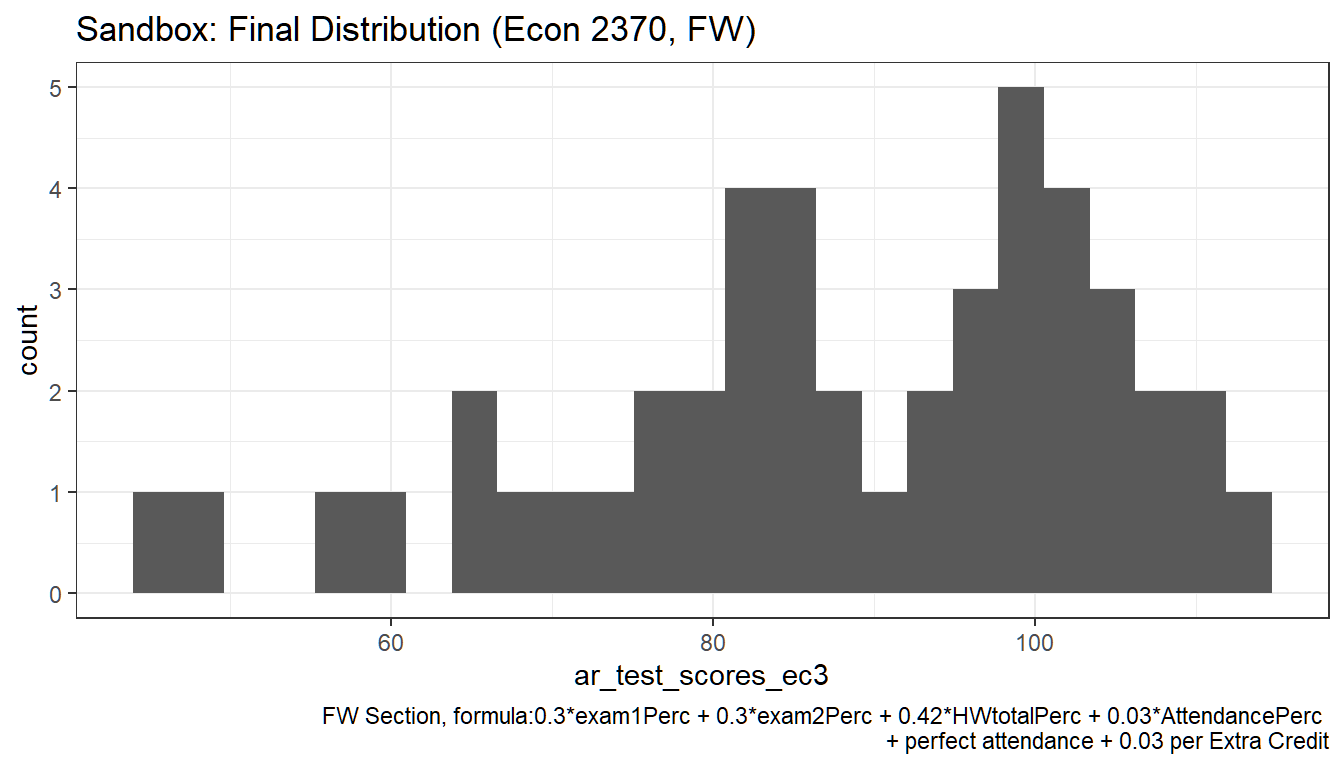
\includegraphics{Panel-Data-and-Optimization-with-R_files/figure-latex/unnamed-chunk-68-1} \end{center}

\begin{Shaded}
\begin{Highlighting}[]
\KeywordTok{ggplot}\NormalTok{(tb_test_data, }\KeywordTok{aes}\NormalTok{(}\DataTypeTok{x=}\NormalTok{exam_score)) }\OperatorTok{+}
\StringTok{  }\KeywordTok{geom_histogram}\NormalTok{(}\DataTypeTok{bins=}\DecValTok{16}\NormalTok{) }\OperatorTok{+}
\StringTok{  }\KeywordTok{labs}\NormalTok{(}\DataTypeTok{title =} \KeywordTok{paste0}\NormalTok{(}\StringTok{'Exam Distribution'}\NormalTok{),}
       \DataTypeTok{caption =} \StringTok{'All Sections'}\NormalTok{) }\OperatorTok{+}
\StringTok{  }\KeywordTok{theme_bw}\NormalTok{()}
\end{Highlighting}
\end{Shaded}

\begin{center}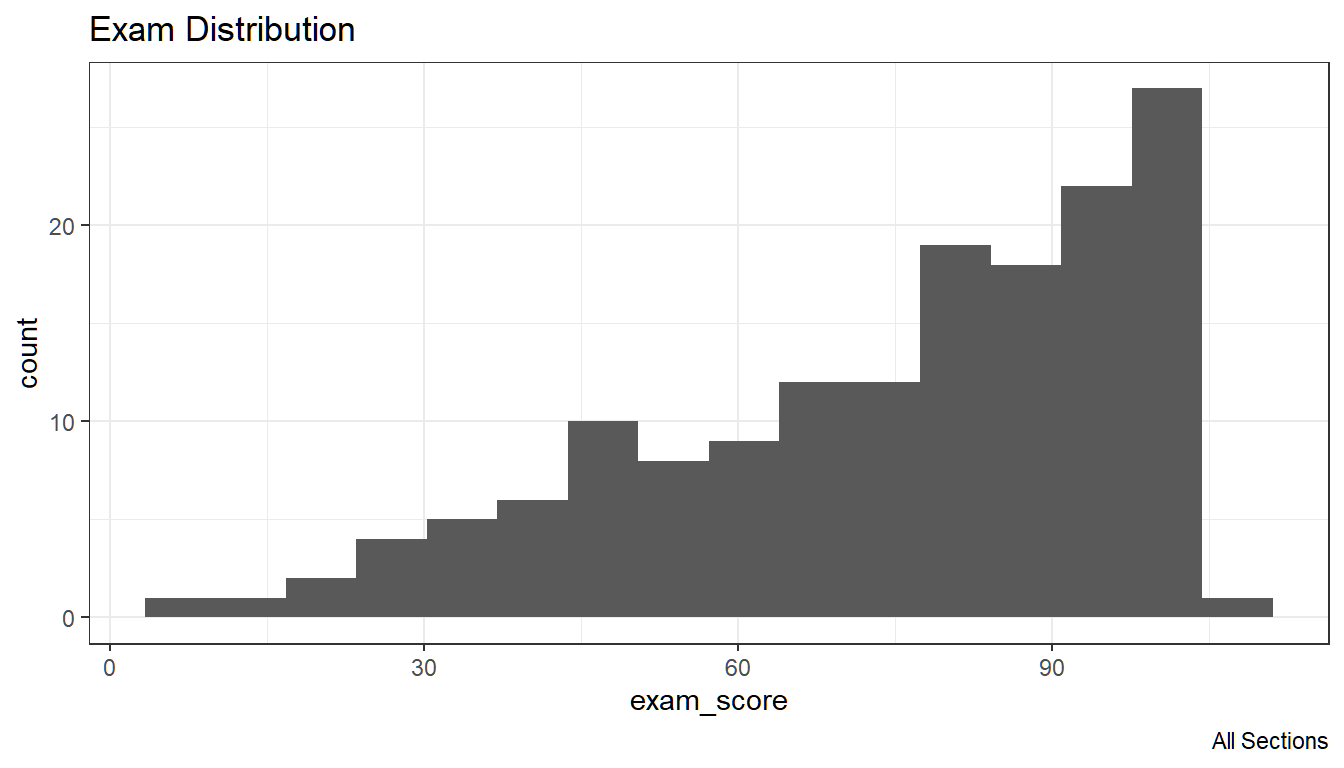
\includegraphics{Panel-Data-and-Optimization-with-R_files/figure-latex/unnamed-chunk-69-1} \end{center}

\hypertarget{summarize-multiple-variables}{%
\section{Summarize Multiple Variables}\label{summarize-multiple-variables}}

\hypertarget{generate-replace-variables}{%
\subsection{Generate Replace Variables}\label{generate-replace-variables}}

\begin{quote}
Go back to \href{http://fanwangecon.github.io/}{fan}'s \href{https://fanwangecon.github.io/REconTools/}{REconTools} Package, \href{https://fanwangecon.github.io/R4Econ/}{R4Econ} Repository (\href{https://fanwangecon.github.io/R4Econ/bookdown}{bookdown site}), or \href{https://fanwangecon.github.io/Stat4Econ/}{Intro Stats with R} Repository.
\end{quote}

\hypertarget{replace-na-for-multiple-variables}{%
\subsubsection{Replace NA for Multiple Variables}\label{replace-na-for-multiple-variables}}

Replace some variables NA by some values, and other variables' NAs by other values.

\begin{Shaded}
\begin{Highlighting}[]
\CommentTok{# Define}
\NormalTok{it_N <-}\StringTok{ }\DecValTok{3}
\NormalTok{it_M <-}\StringTok{ }\DecValTok{5}
\NormalTok{svr_id <-}\StringTok{ 'date'}

\CommentTok{# NA dataframe}
\NormalTok{df_NA <-}\StringTok{ }\KeywordTok{as_tibble}\NormalTok{(}\KeywordTok{matrix}\NormalTok{(}\OtherTok{NA}\NormalTok{, }\DataTypeTok{nrow=}\NormalTok{it_N, }\DataTypeTok{ncol=}\NormalTok{it_M)) }\OperatorTok
\StringTok{  }\KeywordTok{rowid_to_column}\NormalTok{(}\DataTypeTok{var =}\NormalTok{ svr_id) }\OperatorTok
\StringTok{  }\KeywordTok{rename_at}\NormalTok{(}\KeywordTok{vars}\NormalTok{(}\KeywordTok{starts_with}\NormalTok{(}\StringTok{"V"}\NormalTok{)),}
            \KeywordTok{funs}\NormalTok{(}\KeywordTok{str_replace}\NormalTok{(., }\StringTok{"V"}\NormalTok{, }\StringTok{"var"}\NormalTok{)))}
\KeywordTok{kable}\NormalTok{(df_NA) }\OperatorTok
\StringTok{  }\KeywordTok{kable_styling_fc}\NormalTok{()}
\end{Highlighting}
\end{Shaded}

\begin{table}[!h]
\centering
\begin{tabular}{r|l|l|l|l|l}
\hline
date & var1 & var2 & var3 & var4 & var5\\
\hline
\rowcolor{gray!6}  1 & NA & NA & NA & NA & NA\\
\hline
2 & NA & NA & NA & NA & NA\\
\hline
\rowcolor{gray!6}  3 & NA & NA & NA & NA & NA\\
\hline
\end{tabular}
\end{table}

\begin{Shaded}
\begin{Highlighting}[]
\CommentTok{# Replace NA}
\NormalTok{df_NA_replace <-}\StringTok{ }\NormalTok{df_NA }\OperatorTok
\StringTok{  }\KeywordTok{mutate_at}\NormalTok{(}\KeywordTok{vars}\NormalTok{(}\KeywordTok{one_of}\NormalTok{(}\KeywordTok{c}\NormalTok{(}\StringTok{'var1'}\NormalTok{, }\StringTok{'var2'}\NormalTok{))), }\KeywordTok{list}\NormalTok{(}\OperatorTok{~}\KeywordTok{replace_na}\NormalTok{(., }\DecValTok{0}\NormalTok{))) }\OperatorTok
\StringTok{  }\KeywordTok{mutate_at}\NormalTok{(}\KeywordTok{vars}\NormalTok{(}\KeywordTok{one_of}\NormalTok{(}\KeywordTok{c}\NormalTok{(}\StringTok{'var3'}\NormalTok{, }\StringTok{'var5'}\NormalTok{))), }\KeywordTok{list}\NormalTok{(}\OperatorTok{~}\KeywordTok{replace_na}\NormalTok{(., }\DecValTok{99}\NormalTok{)))}
\KeywordTok{kable}\NormalTok{(df_NA_replace) }\OperatorTok
\StringTok{  }\KeywordTok{kable_styling_fc}\NormalTok{()}
\end{Highlighting}
\end{Shaded}

\begin{table}[!h]
\centering
\begin{tabular}{r|r|r|r|l|r}
\hline
date & var1 & var2 & var3 & var4 & var5\\
\hline
\rowcolor{gray!6}  1 & 0 & 0 & 99 & NA & 99\\
\hline
2 & 0 & 0 & 99 & NA & 99\\
\hline
\rowcolor{gray!6}  3 & 0 & 0 & 99 & NA & 99\\
\hline
\end{tabular}
\end{table}

\hypertarget{cumulative-sum-multiple-variables}{%
\subsubsection{Cumulative Sum Multiple Variables}\label{cumulative-sum-multiple-variables}}

Each row is a different date, each column is the profit a firms earns on a date, we want to compute cumulatively how much a person is earning. Also renames variable names below jointly.

\begin{Shaded}
\begin{Highlighting}[]
\CommentTok{# Define}
\NormalTok{it_N <-}\StringTok{ }\DecValTok{3}
\NormalTok{it_M <-}\StringTok{ }\DecValTok{5}
\NormalTok{svr_id <-}\StringTok{ 'date'}

\CommentTok{# random dataframe, daily profit of firms}
\CommentTok{# dp_fx: daily profit firm ID something}
\KeywordTok{set.seed}\NormalTok{(}\DecValTok{123}\NormalTok{)}
\NormalTok{df_daily_profit <-}\StringTok{ }\KeywordTok{as_tibble}\NormalTok{(}\KeywordTok{matrix}\NormalTok{(}\KeywordTok{rnorm}\NormalTok{(it_N}\OperatorTok{*}\NormalTok{it_M), }\DataTypeTok{nrow=}\NormalTok{it_N, }\DataTypeTok{ncol=}\NormalTok{it_M)) }\OperatorTok
\StringTok{  }\KeywordTok{rowid_to_column}\NormalTok{(}\DataTypeTok{var =}\NormalTok{ svr_id) }\OperatorTok
\StringTok{  }\KeywordTok{rename_at}\NormalTok{(}\KeywordTok{vars}\NormalTok{(}\KeywordTok{starts_with}\NormalTok{(}\StringTok{"V"}\NormalTok{)),}
            \KeywordTok{funs}\NormalTok{(}\KeywordTok{str_replace}\NormalTok{(., }\StringTok{"V"}\NormalTok{, }\StringTok{"dp_f"}\NormalTok{)))}
\KeywordTok{kable}\NormalTok{(df_daily_profit) }\OperatorTok
\StringTok{  }\KeywordTok{kable_styling_fc}\NormalTok{()}
\end{Highlighting}
\end{Shaded}

\begin{table}[!h]
\centering
\begin{tabular}{r|r|r|r|r|r}
\hline
date & dp\_f1 & dp\_f2 & dp\_f3 & dp\_f4 & dp\_f5\\
\hline
\rowcolor{gray!6}  1 & -0.5604756 & 0.0705084 & 0.4609162 & -0.4456620 & 0.4007715\\
\hline
2 & -0.2301775 & 0.1292877 & -1.2650612 & 1.2240818 & 0.1106827\\
\hline
\rowcolor{gray!6}  3 & 1.5587083 & 1.7150650 & -0.6868529 & 0.3598138 & -0.5558411\\
\hline
\end{tabular}
\end{table}

\begin{Shaded}
\begin{Highlighting}[]
\CommentTok{# cumulative sum with suffix}
\NormalTok{df_cumu_profit_suffix <-}\StringTok{ }\NormalTok{df_daily_profit }\OperatorTok
\StringTok{  }\KeywordTok{mutate_at}\NormalTok{(}\KeywordTok{vars}\NormalTok{(}\KeywordTok{contains}\NormalTok{(}\StringTok{'dp_f'}\NormalTok{)), }\DataTypeTok{.funs =} \KeywordTok{list}\NormalTok{(}\DataTypeTok{cumu =} \OperatorTok{~}\KeywordTok{cumsum}\NormalTok{(.)))}
\KeywordTok{kable}\NormalTok{(df_cumu_profit_suffix) }\OperatorTok
\StringTok{  }\KeywordTok{kable_styling_fc_wide}\NormalTok{()}
\end{Highlighting}
\end{Shaded}

\begin{table}[!h]
\centering
\resizebox{\linewidth}{!}{
\begin{tabular}{r|r|r|r|r|r|r|r|r|r|r}
\hline
date & dp\_f1 & dp\_f2 & dp\_f3 & dp\_f4 & dp\_f5 & dp\_f1\_cumu & dp\_f2\_cumu & dp\_f3\_cumu & dp\_f4\_cumu & dp\_f5\_cumu\\
\hline
\rowcolor{gray!6}  1 & -0.5604756 & 0.0705084 & 0.4609162 & -0.4456620 & 0.4007715 & -0.5604756 & 0.0705084 & 0.4609162 & -0.4456620 & 0.4007715\\
\hline
2 & -0.2301775 & 0.1292877 & -1.2650612 & 1.2240818 & 0.1106827 & -0.7906531 & 0.1997961 & -0.8041450 & 0.7784198 & 0.5114542\\
\hline
\rowcolor{gray!6}  3 & 1.5587083 & 1.7150650 & -0.6868529 & 0.3598138 & -0.5558411 & 0.7680552 & 1.9148611 & -1.4909979 & 1.1382337 & -0.0443870\\
\hline
\end{tabular}}
\end{table}

\begin{Shaded}
\begin{Highlighting}[]
\CommentTok{# cumulative sum variables naming to prefix}
\NormalTok{df_cumu_profit <-}\StringTok{ }\NormalTok{df_cumu_profit_suffix }\OperatorTok
\StringTok{  }\KeywordTok{rename_at}\NormalTok{(}\KeywordTok{vars}\NormalTok{(}\KeywordTok{contains}\NormalTok{( }\StringTok{"_cumu"}\NormalTok{) ), }\KeywordTok{list}\NormalTok{(}\OperatorTok{~}\KeywordTok{paste}\NormalTok{(}\StringTok{"cp_f"}\NormalTok{, }\KeywordTok{gsub}\NormalTok{(}\StringTok{"_cumu"}\NormalTok{, }\StringTok{""}\NormalTok{, .), }\DataTypeTok{sep =} \StringTok{""}\NormalTok{))) }\OperatorTok
\StringTok{  }\KeywordTok{rename_at}\NormalTok{(}\KeywordTok{vars}\NormalTok{(}\KeywordTok{contains}\NormalTok{( }\StringTok{"cp_f"}\NormalTok{) ), }\KeywordTok{list}\NormalTok{(}\OperatorTok{~}\KeywordTok{gsub}\NormalTok{(}\StringTok{"dp_f"}\NormalTok{, }\StringTok{""}\NormalTok{, .)))}
\KeywordTok{kable}\NormalTok{(df_cumu_profit) }\OperatorTok
\StringTok{  }\KeywordTok{kable_styling_fc_wide}\NormalTok{()}
\end{Highlighting}
\end{Shaded}

\begin{table}[!h]
\centering
\resizebox{\linewidth}{!}{
\begin{tabular}{r|r|r|r|r|r|r|r|r|r|r}
\hline
date & dp\_f1 & dp\_f2 & dp\_f3 & dp\_f4 & dp\_f5 & cp\_f1 & cp\_f2 & cp\_f3 & cp\_f4 & cp\_f5\\
\hline
\rowcolor{gray!6}  1 & -0.5604756 & 0.0705084 & 0.4609162 & -0.4456620 & 0.4007715 & -0.5604756 & 0.0705084 & 0.4609162 & -0.4456620 & 0.4007715\\
\hline
2 & -0.2301775 & 0.1292877 & -1.2650612 & 1.2240818 & 0.1106827 & -0.7906531 & 0.1997961 & -0.8041450 & 0.7784198 & 0.5114542\\
\hline
\rowcolor{gray!6}  3 & 1.5587083 & 1.7150650 & -0.6868529 & 0.3598138 & -0.5558411 & 0.7680552 & 1.9148611 & -1.4909979 & 1.1382337 & -0.0443870\\
\hline
\end{tabular}}
\end{table}

\hypertarget{functions}{%
\chapter{Functions}\label{functions}}

\hypertarget{dataframe-mutate}{%
\section{Dataframe Mutate}\label{dataframe-mutate}}

\hypertarget{row-input-functions}{%
\subsection{Row Input Functions}\label{row-input-functions}}

\begin{quote}
Go back to \href{http://fanwangecon.github.io/}{fan}'s \href{https://fanwangecon.github.io/REconTools/}{REconTools} Package, \href{https://fanwangecon.github.io/R4Econ/}{R4Econ} Repository (\href{https://fanwangecon.github.io/R4Econ/bookdown}{bookdown site}), or \href{https://fanwangecon.github.io/Stat4Econ/}{Intro Stats with R} Repository.
\end{quote}

We want evaluate nonlinear function f(Q\_i, y\_i, ar\_x, ar\_y, c, d), where c and d are constants, and ar\_x and ar\_y are arrays, both fixed. x\_i and y\_i vary over each row of matrix. We would like to evaluate this nonlinear function concurrently across \(N\) individuals. The eventual goal is to find the \(i\) specific \(Q\) that solves the nonlinear equations.

This is a continuation of \href{https://fanwangecon.github.io/R4Econ/function/noloop/fs_applysapplymutate.html}{R use Apply, Sapply and dplyr Mutate to Evaluate one Function Across Rows of a Matrix}

\hypertarget{set-up-input-arrays}{%
\subsubsection{Set up Input Arrays}\label{set-up-input-arrays}}

There is a function that takes \(M=Q+P\) inputs, we want to evaluate this function \(N\) times. Each time, there are \(M\) inputs, where all but \(Q\) of the \(M\) inputs, meaning \(P\) of the \(M\) inputs, are the same. In particular, \(P=Q*N\).

\[M = Q+P = Q + Q*N\]

\begin{Shaded}
\begin{Highlighting}[]
\CommentTok{# it_child_count = N, the number of children}
\NormalTok{it_N_child_cnt =}\StringTok{ }\DecValTok{5}
\CommentTok{# it_heter_param = Q, number of parameters that are heterogeneous across children}
\NormalTok{it_Q_hetpa_cnt =}\StringTok{ }\DecValTok{2}

\CommentTok{# P fixed parameters, nN is N dimensional, nP is P dimensional}
\NormalTok{ar_nN_A =}\StringTok{ }\KeywordTok{seq}\NormalTok{(}\OperatorTok{-}\DecValTok{2}\NormalTok{, }\DecValTok{2}\NormalTok{, }\DataTypeTok{length.out =}\NormalTok{ it_N_child_cnt)}
\NormalTok{ar_nN_alpha =}\StringTok{ }\KeywordTok{seq}\NormalTok{(}\FloatTok{0.1}\NormalTok{, }\FloatTok{0.9}\NormalTok{, }\DataTypeTok{length.out =}\NormalTok{ it_N_child_cnt)}
\NormalTok{ar_nP_A_alpha =}\StringTok{ }\KeywordTok{c}\NormalTok{(ar_nN_A, ar_nN_alpha)}
\NormalTok{ar_nN_N_choice =}\StringTok{ }\KeywordTok{seq}\NormalTok{(}\DecValTok{1}\NormalTok{,it_N_child_cnt)}\OperatorTok{/}\KeywordTok{sum}\NormalTok{(}\KeywordTok{seq}\NormalTok{(}\DecValTok{1}\NormalTok{,it_N_child_cnt))}

\CommentTok{# N by Q varying parameters}
\NormalTok{mt_nN_by_nQ_A_alpha =}\StringTok{ }\KeywordTok{cbind}\NormalTok{(ar_nN_A, ar_nN_alpha, ar_nN_N_choice)}
\CommentTok{# Show}
\KeywordTok{kable}\NormalTok{(mt_nN_by_nQ_A_alpha) }\OperatorTok
\StringTok{  }\KeywordTok{kable_styling_fc}\NormalTok{()}
\end{Highlighting}
\end{Shaded}

\begin{table}[!h]
\centering
\begin{tabular}{r|r|r}
\hline
ar\_nN\_A & ar\_nN\_alpha & ar\_nN\_N\_choice\\
\hline
\rowcolor{gray!6}  -2 & 0.1 & 0.0666667\\
\hline
-1 & 0.3 & 0.1333333\\
\hline
\rowcolor{gray!6}  0 & 0.5 & 0.2000000\\
\hline
1 & 0.7 & 0.2666667\\
\hline
\rowcolor{gray!6}  2 & 0.9 & 0.3333333\\
\hline
\end{tabular}
\end{table}

\hypertarget{testing-function}{%
\subsubsection{Testing Function}\label{testing-function}}

Test non-linear Equation.

\begin{Shaded}
\begin{Highlighting}[]
\CommentTok{# Test Parameters}
\NormalTok{fl_N_agg =}\StringTok{ }\DecValTok{100}
\NormalTok{fl_rho =}\StringTok{ }\DecValTok{-1}
\NormalTok{fl_N_q =}\StringTok{ }\NormalTok{ar_nN_N_choice[}\DecValTok{4}\NormalTok{]}\OperatorTok{*}\NormalTok{fl_N_agg}
\NormalTok{ar_A_alpha =}\StringTok{ }\NormalTok{mt_nN_by_nQ_A_alpha[}\DecValTok{4}\NormalTok{,]}
\CommentTok{# Apply Function}
\NormalTok{ar_p1_s1 =}\StringTok{ }\KeywordTok{exp}\NormalTok{((ar_A_alpha[}\DecValTok{1}\NormalTok{] }\OperatorTok{-}\StringTok{ }\NormalTok{ar_nN_A)}\OperatorTok{*}\NormalTok{fl_rho)}
\NormalTok{ar_p1_s2 =}\StringTok{ }\NormalTok{(ar_A_alpha[}\DecValTok{2}\NormalTok{]}\OperatorTok{/}\NormalTok{ar_nN_alpha)}
\NormalTok{ar_p1_s3 =}\StringTok{ }\NormalTok{(}\DecValTok{1}\OperatorTok{/}\NormalTok{(ar_nN_alpha}\OperatorTok{*}\NormalTok{fl_rho }\OperatorTok{-}\StringTok{ }\DecValTok{1}\NormalTok{))}
\NormalTok{ar_p1 =}\StringTok{ }\NormalTok{(ar_p1_s1}\OperatorTok{*}\NormalTok{ar_p1_s2)}\OperatorTok{^}\NormalTok{ar_p1_s3}
\NormalTok{ar_p2 =}\StringTok{ }\NormalTok{fl_N_q}\OperatorTok{^}\NormalTok{((ar_A_alpha[}\DecValTok{2}\NormalTok{]}\OperatorTok{*}\NormalTok{fl_rho}\DecValTok{-1}\NormalTok{)}\OperatorTok{/}\NormalTok{(ar_nN_alpha}\OperatorTok{*}\NormalTok{fl_rho}\DecValTok{-1}\NormalTok{))}
\NormalTok{ar_overall =}\StringTok{ }\NormalTok{ar_p1}\OperatorTok{*}\NormalTok{ar_p2}
\NormalTok{fl_overall =}\StringTok{ }\NormalTok{fl_N_agg }\OperatorTok{-}\StringTok{ }\KeywordTok{sum}\NormalTok{(ar_overall)}
\KeywordTok{print}\NormalTok{(fl_overall)}
\end{Highlighting}
\end{Shaded}

\begin{verbatim}
## [1] -598.2559
\end{verbatim}

Implement the non-linear problem's evaluation using apply over all \(N\) individuals.

\begin{Shaded}
\begin{Highlighting}[]
\CommentTok{# Define Implicit Function}
\NormalTok{ffi_nonlin_dplyrdo <-}\StringTok{ }\ControlFlowTok{function}\NormalTok{(fl_A, fl_alpha, fl_N, ar_A, ar_alpha, fl_N_agg, fl_rho)\{}
  \CommentTok{# ar_A_alpha[1] is A}
  \CommentTok{# ar_A_alpha[2] is alpha}

  \CommentTok{# # Test Parameters}
  \CommentTok{# fl_N = 100}
  \CommentTok{# fl_rho = -1}
  \CommentTok{# fl_N_q = 10}

  \CommentTok{# Apply Function}
\NormalTok{  ar_p1_s1 =}\StringTok{ }\KeywordTok{exp}\NormalTok{((fl_A }\OperatorTok{-}\StringTok{ }\NormalTok{ar_A)}\OperatorTok{*}\NormalTok{fl_rho)}
\NormalTok{  ar_p1_s2 =}\StringTok{ }\NormalTok{(fl_alpha}\OperatorTok{/}\NormalTok{ar_alpha)}
\NormalTok{  ar_p1_s3 =}\StringTok{ }\NormalTok{(}\DecValTok{1}\OperatorTok{/}\NormalTok{(ar_alpha}\OperatorTok{*}\NormalTok{fl_rho }\OperatorTok{-}\StringTok{ }\DecValTok{1}\NormalTok{))}
\NormalTok{  ar_p1 =}\StringTok{ }\NormalTok{(ar_p1_s1}\OperatorTok{*}\NormalTok{ar_p1_s2)}\OperatorTok{^}\NormalTok{ar_p1_s3}
\NormalTok{  ar_p2 =}\StringTok{ }\NormalTok{fl_N}\OperatorTok{^}\NormalTok{((fl_alpha}\OperatorTok{*}\NormalTok{fl_rho}\DecValTok{-1}\NormalTok{)}\OperatorTok{/}\NormalTok{(ar_alpha}\OperatorTok{*}\NormalTok{fl_rho}\DecValTok{-1}\NormalTok{))}
\NormalTok{  ar_overall =}\StringTok{ }\NormalTok{ar_p1}\OperatorTok{*}\NormalTok{ar_p2}
\NormalTok{  fl_overall =}\StringTok{ }\NormalTok{fl_N_agg }\OperatorTok{-}\StringTok{ }\KeywordTok{sum}\NormalTok{(ar_overall)}

  \KeywordTok{return}\NormalTok{(fl_overall)}
\NormalTok{\}}

\CommentTok{# Parameters}
\NormalTok{fl_rho =}\StringTok{ }\DecValTok{-1}

\CommentTok{# Evaluate Function}
\KeywordTok{print}\NormalTok{(}\KeywordTok{ffi_nonlin_dplyrdo}\NormalTok{(mt_nN_by_nQ_A_alpha[}\DecValTok{1}\NormalTok{,}\DecValTok{1}\NormalTok{],}
\NormalTok{                         mt_nN_by_nQ_A_alpha[}\DecValTok{1}\NormalTok{,}\DecValTok{2}\NormalTok{],}
\NormalTok{                         mt_nN_by_nQ_A_alpha[}\DecValTok{1}\NormalTok{,}\DecValTok{3}\NormalTok{]}\OperatorTok{*}\NormalTok{fl_N_agg,}
\NormalTok{                         ar_nN_A, ar_nN_alpha, fl_N_agg, fl_rho))}
\end{Highlighting}
\end{Shaded}

\begin{verbatim}
## [1] 81.86645
\end{verbatim}

\begin{Shaded}
\begin{Highlighting}[]
\ControlFlowTok{for}\NormalTok{ (i }\ControlFlowTok{in} \KeywordTok{seq}\NormalTok{(}\DecValTok{1}\NormalTok{,}\KeywordTok{dim}\NormalTok{(mt_nN_by_nQ_A_alpha)[}\DecValTok{1}\NormalTok{]))\{}
\NormalTok{  fl_eval =}\StringTok{ }\KeywordTok{ffi_nonlin_dplyrdo}\NormalTok{(mt_nN_by_nQ_A_alpha[i,}\DecValTok{1}\NormalTok{],}
\NormalTok{                               mt_nN_by_nQ_A_alpha[i,}\DecValTok{2}\NormalTok{],}
\NormalTok{                               mt_nN_by_nQ_A_alpha[i,}\DecValTok{3}\NormalTok{]}\OperatorTok{*}\NormalTok{fl_N_agg,}
\NormalTok{                               ar_nN_A, ar_nN_alpha, fl_N_agg, fl_rho)}
  \KeywordTok{print}\NormalTok{(fl_eval)}
\NormalTok{\}}
\end{Highlighting}
\end{Shaded}

\begin{verbatim}
## [1] 81.86645
## [1] 54.48885
## [1] -65.5619
## [1] -598.2559
## [1] -3154.072
\end{verbatim}

\hypertarget{evaluate-nonlinear-function-using-dplyr-mutate}{%
\subsubsection{Evaluate Nonlinear Function using dplyr mutate}\label{evaluate-nonlinear-function-using-dplyr-mutate}}

\begin{Shaded}
\begin{Highlighting}[]
\CommentTok{# Convert Matrix to Tibble}
\NormalTok{ar_st_col_names =}\StringTok{ }\KeywordTok{c}\NormalTok{(}\StringTok{'fl_A'}\NormalTok{, }\StringTok{'fl_alpha'}\NormalTok{, }\StringTok{'fl_N'}\NormalTok{)}
\NormalTok{tb_nN_by_nQ_A_alpha <-}\StringTok{ }\KeywordTok{as_tibble}\NormalTok{(mt_nN_by_nQ_A_alpha) }\OperatorTok\StringTok{ }\KeywordTok{rename_all}\NormalTok{(}\OperatorTok{~}\KeywordTok{c}\NormalTok{(ar_st_col_names))}

\CommentTok{# Define Implicit Function}
\NormalTok{ffi_nonlin_dplyrdo <-}\StringTok{ }\ControlFlowTok{function}\NormalTok{(fl_A, fl_alpha, fl_N, ar_A, ar_alpha, fl_N_agg, fl_rho)\{}

  \CommentTok{# Test Parameters}
  \CommentTok{# ar_A = ar_nN_A}
  \CommentTok{# ar_alpha = ar_nN_alpha}
  \CommentTok{# fl_N = 100}
  \CommentTok{# fl_rho = -1}
  \CommentTok{# fl_N_q = 10}

  \CommentTok{# Apply Function}
\NormalTok{  ar_p1_s1 =}\StringTok{ }\KeywordTok{exp}\NormalTok{((fl_A }\OperatorTok{-}\StringTok{ }\NormalTok{ar_A)}\OperatorTok{*}\NormalTok{fl_rho)}
\NormalTok{  ar_p1_s2 =}\StringTok{ }\NormalTok{(fl_alpha}\OperatorTok{/}\NormalTok{ar_alpha)}
\NormalTok{  ar_p1_s3 =}\StringTok{ }\NormalTok{(}\DecValTok{1}\OperatorTok{/}\NormalTok{(ar_alpha}\OperatorTok{*}\NormalTok{fl_rho }\OperatorTok{-}\StringTok{ }\DecValTok{1}\NormalTok{))}
\NormalTok{  ar_p1 =}\StringTok{ }\NormalTok{(ar_p1_s1}\OperatorTok{*}\NormalTok{ar_p1_s2)}\OperatorTok{^}\NormalTok{ar_p1_s3}
\NormalTok{  ar_p2 =}\StringTok{ }\NormalTok{(fl_N}\OperatorTok{*}\NormalTok{fl_N_agg)}\OperatorTok{^}\NormalTok{((fl_alpha}\OperatorTok{*}\NormalTok{fl_rho}\DecValTok{-1}\NormalTok{)}\OperatorTok{/}\NormalTok{(ar_alpha}\OperatorTok{*}\NormalTok{fl_rho}\DecValTok{-1}\NormalTok{))}
\NormalTok{  ar_overall =}\StringTok{ }\NormalTok{ar_p1}\OperatorTok{*}\NormalTok{ar_p2}
\NormalTok{  fl_overall =}\StringTok{ }\NormalTok{fl_N_agg }\OperatorTok{-}\StringTok{ }\KeywordTok{sum}\NormalTok{(ar_overall)}

  \KeywordTok{return}\NormalTok{(fl_overall)}
\NormalTok{\}}

\CommentTok{# fl_A, fl_alpha are from columns of tb_nN_by_nQ_A_alpha}
\NormalTok{tb_nN_by_nQ_A_alpha =}\StringTok{ }\NormalTok{tb_nN_by_nQ_A_alpha }\OperatorTok\StringTok{ }\KeywordTok{rowwise}\NormalTok{() }\OperatorTok
\StringTok{                        }\KeywordTok{mutate}\NormalTok{(}\DataTypeTok{dplyr_eval =} \KeywordTok{ffi_nonlin_dplyrdo}\NormalTok{(fl_A, fl_alpha, fl_N,}
\NormalTok{                                                               ar_nN_A, ar_nN_alpha,}
\NormalTok{                                                               fl_N_agg, fl_rho))}
\CommentTok{# Show}
\KeywordTok{kable}\NormalTok{(tb_nN_by_nQ_A_alpha) }\OperatorTok
\StringTok{  }\KeywordTok{kable_styling_fc}\NormalTok{()}
\end{Highlighting}
\end{Shaded}

\begin{table}[!h]
\centering
\begin{tabular}{r|r|r|r}
\hline
fl\_A & fl\_alpha & fl\_N & dplyr\_eval\\
\hline
\rowcolor{gray!6}  -2 & 0.1 & 0.0666667 & 81.86645\\
\hline
-1 & 0.3 & 0.1333333 & 54.48885\\
\hline
\rowcolor{gray!6}  0 & 0.5 & 0.2000000 & -65.56190\\
\hline
1 & 0.7 & 0.2666667 & -598.25595\\
\hline
\rowcolor{gray!6}  2 & 0.9 & 0.3333333 & -3154.07226\\
\hline
\end{tabular}
\end{table}

\hypertarget{evaluate-choices-across-states}{%
\subsection{Evaluate Choices Across States}\label{evaluate-choices-across-states}}

\begin{quote}
Go back to \href{http://fanwangecon.github.io/}{fan}'s \href{https://fanwangecon.github.io/REconTools/}{REconTools} Package, \href{https://fanwangecon.github.io/R4Econ/}{R4Econ} Repository (\href{https://fanwangecon.github.io/R4Econ/bookdown}{bookdown site}), or \href{https://fanwangecon.github.io/Stat4Econ/}{Intro Stats with R} Repository.
\end{quote}

See the \href{https://fanwangecon.github.io/REconTools/reference/ff_opti_bisect_pmap_multi.html}{ff\_opti\_bisect\_pmap\_multi} function from \href{https://fanwangecon.github.io/}{Fan}'s \emph{\href{https://fanwangecon.github.io/REconTools/}{REconTools}} Package, which provides a resuable function based on the algorithm worked out here.

We want evaluate linear function \(0=f(z_{ij}, x_i, y_i, \textbf{X}, \textbf{Y}, c, d)\). There are \(i\) functions that have \(i\) specific \(x\) and \(y\). For each \(i\) function, we evaluate along a grid of feasible values for \(z\), over \(j\in J\) grid points, potentially looking for the \(j\) that is closest to the root. \(\textbf{X}\) and \(\textbf{Y}\) are arrays common across the \(i\) equations, and \(c\) and \(d\) are constants.

The evaluation strategy is the following, given min and max for \(z\) that are specific for each \(j\), and given common number of grid points, generate a matrix of \(z_{ij}\). Suppose there the number of \(i\) is \(I\), and the number of grid points for \(j\) is \(J\).

\begin{enumerate}
\def\labelenumi{\arabic{enumi}.}
\tightlist
\item
  Generate a \(J \cdot I\) by \(3\) matrix where the columns are \(z,x,y\) as tibble
\item
  Follow \href{https://fanwangecon.github.io/R4Econ/function/mutatef/fs_funceval.html}{this} Mutate to evaluate the \(f(\cdot)\) function.
\item
  Add two categorical columns for grid levels and wich \(i\), \(i\) and \(j\) index. Plot Mutate output evaluated column categorized by \(i\) as color and \(j\) as x-axis.
\end{enumerate}

\hypertarget{set-up-input-arrays-1}{%
\subsubsection{Set up Input Arrays}\label{set-up-input-arrays-1}}

There is a function that takes \(M=Q+P\) inputs, we want to evaluate this function \(N\) times. Each time, there are \(M\) inputs, where all but \(Q\) of the \(M\) inputs, meaning \(P\) of the \(M\) inputs, are the same. In particular, \(P=Q*N\).

\[M = Q+P = Q + Q*N\]

Now we need to expand this by the number of choice grid. Each row, representing one equation, is expanded by the number of choice grids. We are graphically searching, or rather brute force searching, which means if we have 100 individuals, we want to plot out the nonlinear equation for each of these lines, and show graphically where each line crosses zero. We achieve this, by evaluating the equation for each of the 100 individuals along a grid of feasible choices.

In this problem here, the feasible choices are shared across individuals.

\begin{Shaded}
\begin{Highlighting}[]
\CommentTok{# Parameters}
\NormalTok{fl_rho =}\StringTok{ }\FloatTok{0.20}
\NormalTok{svr_id_var =}\StringTok{ 'INDI_ID'}

\CommentTok{# it_child_count = N, the number of children}
\NormalTok{it_N_child_cnt =}\StringTok{ }\DecValTok{4}
\CommentTok{# it_heter_param = Q, number of parameters that are heterogeneous across children}
\NormalTok{it_Q_hetpa_cnt =}\StringTok{ }\DecValTok{2}

\CommentTok{# P fixed parameters, nN is N dimensional, nP is P dimensional}
\NormalTok{ar_nN_A =}\StringTok{ }\KeywordTok{seq}\NormalTok{(}\OperatorTok{-}\DecValTok{2}\NormalTok{, }\DecValTok{2}\NormalTok{, }\DataTypeTok{length.out =}\NormalTok{ it_N_child_cnt)}
\NormalTok{ar_nN_alpha =}\StringTok{ }\KeywordTok{seq}\NormalTok{(}\FloatTok{0.1}\NormalTok{, }\FloatTok{0.9}\NormalTok{, }\DataTypeTok{length.out =}\NormalTok{ it_N_child_cnt)}
\NormalTok{ar_nP_A_alpha =}\StringTok{ }\KeywordTok{c}\NormalTok{(ar_nN_A, ar_nN_alpha)}

\CommentTok{# N by Q varying parameters}
\NormalTok{mt_nN_by_nQ_A_alpha =}\StringTok{ }\KeywordTok{cbind}\NormalTok{(ar_nN_A, ar_nN_alpha)}

\CommentTok{# Choice Grid for nutritional feasible choices for each}
\NormalTok{fl_N_agg =}\StringTok{ }\DecValTok{100}
\NormalTok{fl_N_min =}\StringTok{ }\DecValTok{0}
\NormalTok{it_N_choice_cnt_ttest =}\StringTok{ }\DecValTok{3}
\NormalTok{it_N_choice_cnt_dense =}\StringTok{ }\DecValTok{100}
\NormalTok{ar_N_choices_ttest =}\StringTok{ }\KeywordTok{seq}\NormalTok{(fl_N_min, fl_N_agg, }\DataTypeTok{length.out =}\NormalTok{ it_N_choice_cnt_ttest)}
\NormalTok{ar_N_choices_dense =}\StringTok{ }\KeywordTok{seq}\NormalTok{(fl_N_min, fl_N_agg, }\DataTypeTok{length.out =}\NormalTok{ it_N_choice_cnt_dense)}

\CommentTok{# Mesh Expand}
\NormalTok{tb_states_choices <-}\StringTok{ }\KeywordTok{as_tibble}\NormalTok{(mt_nN_by_nQ_A_alpha) }\OperatorTok\StringTok{ }\KeywordTok{rowid_to_column}\NormalTok{(}\DataTypeTok{var=}\NormalTok{svr_id_var)}
\NormalTok{tb_states_choices_ttest <-}\StringTok{ }\NormalTok{tb_states_choices }\OperatorTok\StringTok{ }\KeywordTok{expand_grid}\NormalTok{(}\DataTypeTok{choices =}\NormalTok{ ar_N_choices_ttest)}
\NormalTok{tb_states_choices_dense <-}\StringTok{ }\NormalTok{tb_states_choices }\OperatorTok\StringTok{ }\KeywordTok{expand_grid}\NormalTok{(}\DataTypeTok{choices =}\NormalTok{ ar_N_choices_dense)}

\CommentTok{# display}
\KeywordTok{summary}\NormalTok{(tb_states_choices_dense)}
\end{Highlighting}
\end{Shaded}

\begin{verbatim}
##     INDI_ID        ar_nN_A    ar_nN_alpha     choices   
##  Min.   :1.00   Min.   :-2   Min.   :0.1   Min.   :  0  
##  1st Qu.:1.75   1st Qu.:-1   1st Qu.:0.3   1st Qu.: 25  
##  Median :2.50   Median : 0   Median :0.5   Median : 50  
##  Mean   :2.50   Mean   : 0   Mean   :0.5   Mean   : 50  
##  3rd Qu.:3.25   3rd Qu.: 1   3rd Qu.:0.7   3rd Qu.: 75  
##  Max.   :4.00   Max.   : 2   Max.   :0.9   Max.   :100
\end{verbatim}

\begin{Shaded}
\begin{Highlighting}[]
\KeywordTok{kable}\NormalTok{(tb_states_choices_ttest) }\OperatorTok
\StringTok{  }\KeywordTok{kable_styling_fc}\NormalTok{()}
\end{Highlighting}
\end{Shaded}

\begin{table}[!h]
\centering
\begin{tabular}{r|r|r|r}
\hline
INDI\_ID & ar\_nN\_A & ar\_nN\_alpha & choices\\
\hline
\rowcolor{gray!6}  1 & -2.0000000 & 0.1000000 & 0\\
\hline
1 & -2.0000000 & 0.1000000 & 50\\
\hline
\rowcolor{gray!6}  1 & -2.0000000 & 0.1000000 & 100\\
\hline
2 & -0.6666667 & 0.3666667 & 0\\
\hline
\rowcolor{gray!6}  2 & -0.6666667 & 0.3666667 & 50\\
\hline
2 & -0.6666667 & 0.3666667 & 100\\
\hline
\rowcolor{gray!6}  3 & 0.6666667 & 0.6333333 & 0\\
\hline
3 & 0.6666667 & 0.6333333 & 50\\
\hline
\rowcolor{gray!6}  3 & 0.6666667 & 0.6333333 & 100\\
\hline
4 & 2.0000000 & 0.9000000 & 0\\
\hline
\rowcolor{gray!6}  4 & 2.0000000 & 0.9000000 & 50\\
\hline
4 & 2.0000000 & 0.9000000 & 100\\
\hline
\end{tabular}
\end{table}

\hypertarget{apply-same-function-all-rows-some-inputs-row-specific-other-shared}{%
\subsubsection{Apply Same Function all Rows, Some Inputs Row-specific, other Shared}\label{apply-same-function-all-rows-some-inputs-row-specific-other-shared}}

There are two types of inputs, row-specific inputs, and inputs that should be applied for each row. The Function just requires all of these inputs, it does not know what is row-specific and what is common for all row. Dplyr recognizes which parameter inputs already existing in the piped dataframe/tibble, given rowwise, those will be row-specific inputs. Additional function parameters that do not exist in dataframe as variable names, but that are pre-defined scalars or arrays will be applied to all rows.

\begin{itemize}
\tightlist
\item
  \citet{param} string variable name of input where functions are evaluated, these are already contained in the dataframe, existing variable names, row specific, rowwise computation over these, each rowwise calculation using different rows: \emph{fl\_A}, \emph{fl\_alpha}, \emph{fl\_N}
\item
  \citet{param} scalar and array values that are applied to every rowwise calculation, all rowwise calculations using the same scalars and arrays:\emph{ar\_A}, \emph{ar\_alpha}, \emph{fl\_N\_agg}, \emph{fl\_rho}
\item
  \citet{param} string output variable name
\end{itemize}

The function looks within group, finds min/max etc that are relevant.

\hypertarget{points-and-denser-dataframs-and-define-function}{%
\paragraph{3 Points and Denser Dataframs and Define Function}\label{points-and-denser-dataframs-and-define-function}}

\begin{Shaded}
\begin{Highlighting}[]
\CommentTok{# Convert Matrix to Tibble}
\NormalTok{ar_st_col_names =}\StringTok{ }\KeywordTok{c}\NormalTok{(svr_id_var,}\StringTok{'fl_A'}\NormalTok{, }\StringTok{'fl_alpha'}\NormalTok{)}
\NormalTok{tb_states_choices <-}\StringTok{ }\NormalTok{tb_states_choices }\OperatorTok\StringTok{ }\KeywordTok{rename_all}\NormalTok{(}\OperatorTok{~}\KeywordTok{c}\NormalTok{(ar_st_col_names))}
\NormalTok{ar_st_col_names =}\StringTok{ }\KeywordTok{c}\NormalTok{(svr_id_var,}\StringTok{'fl_A'}\NormalTok{, }\StringTok{'fl_alpha'}\NormalTok{, }\StringTok{'fl_N'}\NormalTok{)}
\NormalTok{tb_states_choices_ttest <-}\StringTok{ }\NormalTok{tb_states_choices_ttest }\OperatorTok\StringTok{ }\KeywordTok{rename_all}\NormalTok{(}\OperatorTok{~}\KeywordTok{c}\NormalTok{(ar_st_col_names))}
\NormalTok{tb_states_choices_dense <-}\StringTok{ }\NormalTok{tb_states_choices_dense }\OperatorTok\StringTok{ }\KeywordTok{rename_all}\NormalTok{(}\OperatorTok{~}\KeywordTok{c}\NormalTok{(ar_st_col_names))}

\CommentTok{# Define Implicit Function}
\NormalTok{ffi_nonlin_dplyrdo <-}\StringTok{ }\ControlFlowTok{function}\NormalTok{(fl_A, fl_alpha, fl_N, ar_A, ar_alpha, fl_N_agg, fl_rho)\{}
  \CommentTok{# scalar value that are row-specific, in dataframe already: *fl_A*, *fl_alpha*, *fl_N*}
  \CommentTok{# array and scalars not in dataframe, common all rows: *ar_A*, *ar_alpha*, *fl_N_agg*, *fl_rho*}

  \CommentTok{# Test Parameters}
  \CommentTok{# ar_A = ar_nN_A}
  \CommentTok{# ar_alpha = ar_nN_alpha}
  \CommentTok{# fl_N = 100}
  \CommentTok{# fl_rho = -1}
  \CommentTok{# fl_N_q = 10}

  \CommentTok{# Apply Function}
\NormalTok{  ar_p1_s1 =}\StringTok{ }\KeywordTok{exp}\NormalTok{((fl_A }\OperatorTok{-}\StringTok{ }\NormalTok{ar_A)}\OperatorTok{*}\NormalTok{fl_rho)}
\NormalTok{  ar_p1_s2 =}\StringTok{ }\NormalTok{(fl_alpha}\OperatorTok{/}\NormalTok{ar_alpha)}
\NormalTok{  ar_p1_s3 =}\StringTok{ }\NormalTok{(}\DecValTok{1}\OperatorTok{/}\NormalTok{(ar_alpha}\OperatorTok{*}\NormalTok{fl_rho }\OperatorTok{-}\StringTok{ }\DecValTok{1}\NormalTok{))}
\NormalTok{  ar_p1 =}\StringTok{ }\NormalTok{(ar_p1_s1}\OperatorTok{*}\NormalTok{ar_p1_s2)}\OperatorTok{^}\NormalTok{ar_p1_s3}
\NormalTok{  ar_p2 =}\StringTok{ }\NormalTok{fl_N}\OperatorTok{^}\NormalTok{((fl_alpha}\OperatorTok{*}\NormalTok{fl_rho}\DecValTok{-1}\NormalTok{)}\OperatorTok{/}\NormalTok{(ar_alpha}\OperatorTok{*}\NormalTok{fl_rho}\DecValTok{-1}\NormalTok{))}
\NormalTok{  ar_overall =}\StringTok{ }\NormalTok{ar_p1}\OperatorTok{*}\NormalTok{ar_p2}
\NormalTok{  fl_overall =}\StringTok{ }\NormalTok{fl_N_agg }\OperatorTok{-}\StringTok{ }\KeywordTok{sum}\NormalTok{(ar_overall)}

  \KeywordTok{return}\NormalTok{(fl_overall)}
\NormalTok{\}}
\end{Highlighting}
\end{Shaded}

\hypertarget{evaluate-at-three-choice-points-and-show-table}{%
\paragraph{Evaluate at Three Choice Points and Show Table}\label{evaluate-at-three-choice-points-and-show-table}}

In the example below, just show results evaluating over three choice points and show table.

\begin{Shaded}
\begin{Highlighting}[]
\CommentTok{# fl_A, fl_alpha are from columns of tb_nN_by_nQ_A_alpha}
\NormalTok{tb_states_choices_ttest_eval =}\StringTok{ }\NormalTok{tb_states_choices_ttest }\OperatorTok\StringTok{ }\KeywordTok{rowwise}\NormalTok{() }\OperatorTok
\StringTok{                        }\KeywordTok{mutate}\NormalTok{(}\DataTypeTok{dplyr_eval =} \KeywordTok{ffi_nonlin_dplyrdo}\NormalTok{(fl_A, fl_alpha, fl_N,}
\NormalTok{                                                               ar_nN_A, ar_nN_alpha,}
\NormalTok{                                                               fl_N_agg, fl_rho))}
\CommentTok{# Show}
\KeywordTok{kable}\NormalTok{(tb_states_choices_ttest_eval) }\OperatorTok
\StringTok{  }\KeywordTok{kable_styling_fc}\NormalTok{()}
\end{Highlighting}
\end{Shaded}

\begin{table}[!h]
\centering
\begin{tabular}{r|r|r|r|r}
\hline
INDI\_ID & fl\_A & fl\_alpha & fl\_N & dplyr\_eval\\
\hline
\rowcolor{gray!6}  1 & -2.0000000 & 0.1000000 & 0 & 100.00000\\
\hline
1 & -2.0000000 & 0.1000000 & 50 & -5666.95576\\
\hline
\rowcolor{gray!6}  1 & -2.0000000 & 0.1000000 & 100 & -12880.28392\\
\hline
2 & -0.6666667 & 0.3666667 & 0 & 100.00000\\
\hline
\rowcolor{gray!6}  2 & -0.6666667 & 0.3666667 & 50 & -595.73454\\
\hline
2 & -0.6666667 & 0.3666667 & 100 & -1394.70698\\
\hline
\rowcolor{gray!6}  3 & 0.6666667 & 0.6333333 & 0 & 100.00000\\
\hline
3 & 0.6666667 & 0.6333333 & 50 & -106.51058\\
\hline
\rowcolor{gray!6}  3 & 0.6666667 & 0.6333333 & 100 & -323.94216\\
\hline
4 & 2.0000000 & 0.9000000 & 0 & 100.00000\\
\hline
\rowcolor{gray!6}  4 & 2.0000000 & 0.9000000 & 50 & 22.55577\\
\hline
4 & 2.0000000 & 0.9000000 & 100 & -51.97161\\
\hline
\end{tabular}
\end{table}

\hypertarget{evaluate-at-many-choice-points-and-show-graphically}{%
\paragraph{Evaluate at Many Choice Points and Show Graphically}\label{evaluate-at-many-choice-points-and-show-graphically}}

Same as above, but now we evaluate the function over the individuals at many choice points so that we can graph things out.

\begin{Shaded}
\begin{Highlighting}[]
\CommentTok{# fl_A, fl_alpha are from columns of tb_nN_by_nQ_A_alpha}
\NormalTok{tb_states_choices_dense_eval =}\StringTok{ }\NormalTok{tb_states_choices_dense }\OperatorTok\StringTok{ }\KeywordTok{rowwise}\NormalTok{() }\OperatorTok
\StringTok{                        }\KeywordTok{mutate}\NormalTok{(}\DataTypeTok{dplyr_eval =} \KeywordTok{ffi_nonlin_dplyrdo}\NormalTok{(fl_A, fl_alpha, fl_N,}
\NormalTok{                                                               ar_nN_A, ar_nN_alpha,}
\NormalTok{                                                               fl_N_agg, fl_rho))}
\end{Highlighting}
\end{Shaded}

\begin{Shaded}
\begin{Highlighting}[]
\CommentTok{# Show}
\KeywordTok{dim}\NormalTok{(tb_states_choices_dense_eval)}
\end{Highlighting}
\end{Shaded}

\begin{verbatim}
## [1] 400   5
\end{verbatim}

\begin{Shaded}
\begin{Highlighting}[]
\KeywordTok{summary}\NormalTok{(tb_states_choices_dense_eval)}
\end{Highlighting}
\end{Shaded}

\begin{verbatim}
##     INDI_ID          fl_A       fl_alpha        fl_N       dplyr_eval       
##  Min.   :1.00   Min.   :-2   Min.   :0.1   Min.   :  0   Min.   :-12880.28  
##  1st Qu.:1.75   1st Qu.:-1   1st Qu.:0.3   1st Qu.: 25   1st Qu.: -1167.29  
##  Median :2.50   Median : 0   Median :0.5   Median : 50   Median :  -202.42  
##  Mean   :2.50   Mean   : 0   Mean   :0.5   Mean   : 50   Mean   : -1645.65  
##  3rd Qu.:3.25   3rd Qu.: 1   3rd Qu.:0.7   3rd Qu.: 75   3rd Qu.:     0.96  
##  Max.   :4.00   Max.   : 2   Max.   :0.9   Max.   :100   Max.   :   100.00
\end{verbatim}

\begin{Shaded}
\begin{Highlighting}[]
\NormalTok{lineplot <-}\StringTok{ }\NormalTok{tb_states_choices_dense_eval }\OperatorTok
\StringTok{    }\KeywordTok{ggplot}\NormalTok{(}\KeywordTok{aes}\NormalTok{(}\DataTypeTok{x=}\NormalTok{fl_N, }\DataTypeTok{y=}\NormalTok{dplyr_eval)) }\OperatorTok{+}
\StringTok{        }\KeywordTok{geom_line}\NormalTok{() }\OperatorTok{+}
\StringTok{        }\KeywordTok{facet_wrap}\NormalTok{( . }\OperatorTok{~}\StringTok{ }\NormalTok{INDI_ID, }\DataTypeTok{scales =} \StringTok{"free"}\NormalTok{) }\OperatorTok{+}
\StringTok{        }\KeywordTok{geom_hline}\NormalTok{(}\DataTypeTok{yintercept=}\DecValTok{0}\NormalTok{, }\DataTypeTok{linetype=}\StringTok{"dashed"}\NormalTok{,}
                \DataTypeTok{color =} \StringTok{"red"}\NormalTok{, }\DataTypeTok{size=}\DecValTok{1}\NormalTok{)}
        \KeywordTok{labs}\NormalTok{(}\DataTypeTok{title =} \StringTok{'Evaluate Non-Linear Functions to Search for Roots'}\NormalTok{,}
             \DataTypeTok{x =} \StringTok{'X values'}\NormalTok{,}
             \DataTypeTok{y =} \StringTok{'f(x)'}\NormalTok{,}
             \DataTypeTok{caption =} \StringTok{'Evaluating the Function'}\NormalTok{)}
\end{Highlighting}
\end{Shaded}

\begin{verbatim}
## $x
## [1] "X values"
## 
## $y
## [1] "f(x)"
## 
## $title
## [1] "Evaluate Non-Linear Functions to Search for Roots"
## 
## $caption
## [1] "Evaluating the Function"
## 
## attr(,"class")
## [1] "labels"
\end{verbatim}

\begin{Shaded}
\begin{Highlighting}[]
\KeywordTok{print}\NormalTok{(lineplot)}
\end{Highlighting}
\end{Shaded}

\begin{center}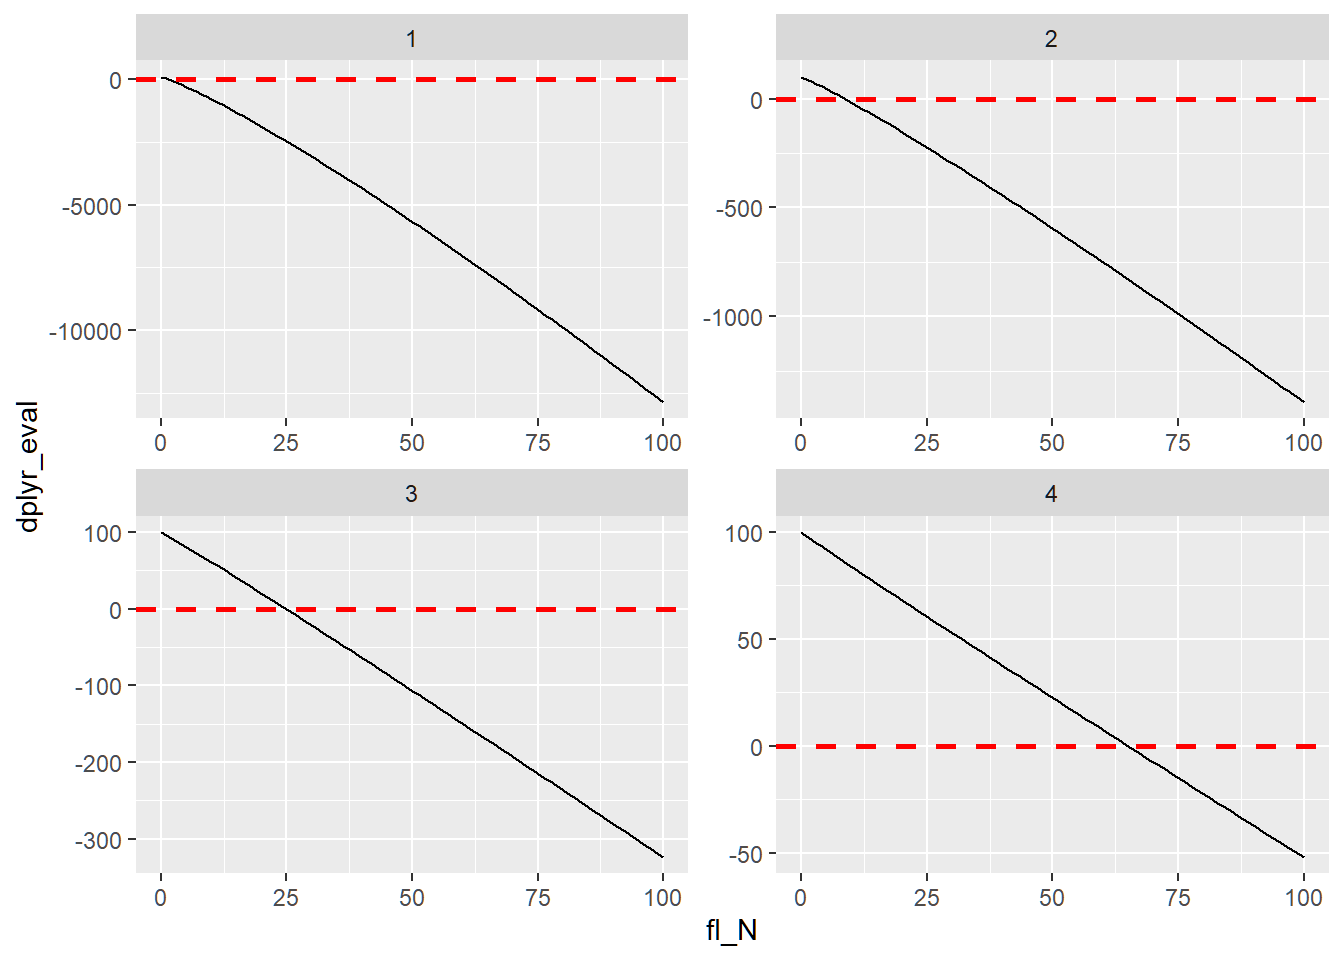
\includegraphics{Panel-Data-and-Optimization-with-R_files/figure-latex/graph many evaluations-1} \end{center}

\hypertarget{dataframe-do-anything}{%
\section{Dataframe Do Anything}\label{dataframe-do-anything}}

\hypertarget{mxq-to-mxp-rows}{%
\subsection{MxQ to MxP Rows}\label{mxq-to-mxp-rows}}

\begin{quote}
Go back to \href{http://fanwangecon.github.io/}{fan}'s \href{https://fanwangecon.github.io/REconTools/}{REconTools} Package, \href{https://fanwangecon.github.io/R4Econ/}{R4Econ} Repository (\href{https://fanwangecon.github.io/R4Econ/bookdown}{bookdown site}), or \href{https://fanwangecon.github.io/Stat4Econ/}{Intro Stats with R} Repository.
\end{quote}

\hypertarget{mxq-to-mx1-rows-within-group-gini}{%
\subsubsection{MxQ to Mx1 Rows: Within Group Gini}\label{mxq-to-mx1-rows-within-group-gini}}

There is a Panel with \(M\) individuals and each individual has \(Q\) records/rows. A function generate an individual specific outcome given the \(Q\) individual specific inputs, along with shared parameters and arrays across the \(M\) individuals.

For example, suppose we have a dataframe of individual wage information from different countries, each row is an individual from one country. We want to generate country specific gini based on the individual data for each country in the dataframe. But additionally, perhaps the gini formula requires not just individual income but some additional parameters or shared dataframes as inputs.

Given the within \(m\) income observations, we can compute gini statistics that are individual specific based on the observed distribution of incomes. For this, we will use the \href{https://fanwangecon.github.io/REconTools/reference/ff_dist_gini_vector_pos.html}{ff\_dist\_gini\_vector\_pos.html} function from \href{https://fanwangecon.github.io/REconTools/}{REconTools}.

To make this more interesting, we will generate large dataframe with more \(M\) and more \(Q\) each \(m\).

\hypertarget{large-dataframe}{%
\paragraph{Large Dataframe}\label{large-dataframe}}

There are up to ten thousand income observation per person. And there are ten people.

\begin{Shaded}
\begin{Highlighting}[]
\CommentTok{# Parameter Setups}
\NormalTok{it_M <-}\StringTok{ }\DecValTok{10}
\NormalTok{it_Q_max <-}\StringTok{ }\DecValTok{10000}
\NormalTok{fl_rnorm_mu <-}\StringTok{ }\DecValTok{1}
\NormalTok{ar_rnorm_sd <-}\StringTok{ }\KeywordTok{seq}\NormalTok{(}\FloatTok{0.01}\NormalTok{, }\FloatTok{0.2}\NormalTok{, }\DataTypeTok{length.out=}\NormalTok{it_M)}
\NormalTok{ar_it_q <-}\StringTok{ }\KeywordTok{sample.int}\NormalTok{(it_Q_max, it_M, }\DataTypeTok{replace=}\OtherTok{TRUE}\NormalTok{)}

\CommentTok{# N by Q varying parameters}
\NormalTok{mt_data =}\StringTok{ }\KeywordTok{cbind}\NormalTok{(ar_it_q, ar_rnorm_sd)}
\NormalTok{tb_M <-}\StringTok{ }\KeywordTok{as_tibble}\NormalTok{(mt_data) }\OperatorTok\StringTok{ }\KeywordTok{rowid_to_column}\NormalTok{(}\DataTypeTok{var =} \StringTok{"ID"}\NormalTok{) }\OperatorTok
\StringTok{                }\KeywordTok{rename}\NormalTok{(}\DataTypeTok{sd =}\NormalTok{ ar_rnorm_sd, }\DataTypeTok{Q =}\NormalTok{ ar_it_q) }\OperatorTok
\StringTok{                }\KeywordTok{mutate}\NormalTok{(}\DataTypeTok{mean =}\NormalTok{ fl_rnorm_mu)}
\end{Highlighting}
\end{Shaded}

\hypertarget{compute-group-specific-gini-normal}{%
\paragraph{Compute Group specific gini, NORMAL}\label{compute-group-specific-gini-normal}}

There is only one input for the gini function \emph{ar\_pos}. Note that the gini are not very large even with large SD, because these are normal distributions. By Construction, most peple are in the middle. So with almost zero standard deviation, we have perfect equality, as standard deviation increases, inequality increases, but still pretty equal overall, there is no fat upper tail.

Note that there are three ways of referring to variable names with dot, which are all shown below:

\begin{enumerate}
\def\labelenumi{\arabic{enumi}.}
\tightlist
\item
  We can explicitly refer to names
\item
  We can use the \href{https://stackoverflow.com/a/18228613/8280804}{dollar dot structure} to use string variable names in do anything.
\item
  We can use dot bracket, this is the only option that works with string variable names
\end{enumerate}

\begin{Shaded}
\begin{Highlighting}[]
\CommentTok{# A. Normal Draw Expansion, Explicitly Name}
\KeywordTok{set.seed}\NormalTok{(}\StringTok{'123'}\NormalTok{)}
\NormalTok{tb_income_norm_dot_dollar <-}\StringTok{ }\NormalTok{tb_M }\OperatorTok\StringTok{ }\KeywordTok{group_by}\NormalTok{(ID) }\OperatorTok
\StringTok{  }\KeywordTok{do}\NormalTok{(}\DataTypeTok{income =} \KeywordTok{rnorm}\NormalTok{(.}\OperatorTok{$}\NormalTok{Q,}
                    \DataTypeTok{mean=}\NormalTok{.}\OperatorTok{$}\NormalTok{mean,}
                    \DataTypeTok{sd=}\NormalTok{.}\OperatorTok{$}\NormalTok{sd)) }\OperatorTok
\StringTok{  }\KeywordTok{unnest}\NormalTok{(}\KeywordTok{c}\NormalTok{(income)) }\OperatorTok
\StringTok{  }\KeywordTok{left_join}\NormalTok{(tb_M, }\DataTypeTok{by=}\StringTok{"ID"}\NormalTok{)}

\CommentTok{# Normal Draw Expansion again, dot dollar differently with string variable name}
\KeywordTok{set.seed}\NormalTok{(}\StringTok{'123'}\NormalTok{)}
\NormalTok{tb_income_norm_dollar_dot <-}\StringTok{ }\NormalTok{tb_M }\OperatorTok\StringTok{ }\KeywordTok{group_by}\NormalTok{(ID) }\OperatorTok
\StringTok{  }\KeywordTok{do}\NormalTok{(}\DataTypeTok{income =} \KeywordTok{rnorm}\NormalTok{(}\StringTok{`}\DataTypeTok{$}\StringTok{`}\NormalTok{(., }\StringTok{'Q'}\NormalTok{),}
                    \DataTypeTok{mean =} \StringTok{`}\DataTypeTok{$}\StringTok{`}\NormalTok{(., }\StringTok{'mean'}\NormalTok{),}
                    \DataTypeTok{sd =} \StringTok{`}\DataTypeTok{$}\StringTok{`}\NormalTok{(., }\StringTok{'sd'}\NormalTok{))) }\OperatorTok
\StringTok{  }\KeywordTok{unnest}\NormalTok{(}\KeywordTok{c}\NormalTok{(income)) }\OperatorTok
\StringTok{  }\KeywordTok{left_join}\NormalTok{(tb_M, }\DataTypeTok{by=}\StringTok{"ID"}\NormalTok{)}

\CommentTok{# Normal Draw Expansion again, dot double bracket}
\KeywordTok{set.seed}\NormalTok{(}\StringTok{'123'}\NormalTok{)}
\NormalTok{svr_mean <-}\StringTok{ 'mean'}
\NormalTok{svr_sd <-}\StringTok{ 'sd'}
\NormalTok{svr_Q <-}\StringTok{ 'Q'}
\NormalTok{tb_income_norm_dot_bracket_db <-}\StringTok{ }\NormalTok{tb_M }\OperatorTok\StringTok{ }\KeywordTok{group_by}\NormalTok{(ID) }\OperatorTok
\StringTok{  }\KeywordTok{do}\NormalTok{(}\DataTypeTok{income =} \KeywordTok{rnorm}\NormalTok{(.[[svr_Q]],}
                    \DataTypeTok{mean =}\NormalTok{ .[[svr_mean]],}
                    \DataTypeTok{sd =}\NormalTok{ .[[svr_sd]])) }\OperatorTok
\StringTok{  }\KeywordTok{unnest}\NormalTok{(}\KeywordTok{c}\NormalTok{(income)) }\OperatorTok
\StringTok{  }\KeywordTok{left_join}\NormalTok{(tb_M, }\DataTypeTok{by=}\StringTok{"ID"}\NormalTok{)}

\CommentTok{# display}
\KeywordTok{sum}\NormalTok{(}\KeywordTok{sum}\NormalTok{(tb_income_norm_dollar_dot }\OperatorTok{-}\StringTok{ }\NormalTok{tb_income_norm_dot_dollar }\OperatorTok{-}\StringTok{ }\NormalTok{tb_income_norm_dot_bracket_db))}
\end{Highlighting}
\end{Shaded}

\begin{verbatim}
## [1] -463785175
\end{verbatim}

\begin{Shaded}
\begin{Highlighting}[]
\CommentTok{# display}
\KeywordTok{head}\NormalTok{(tb_income_norm_dot_dollar, }\DecValTok{20}\NormalTok{)}
\end{Highlighting}
\end{Shaded}

\begin{verbatim}
## # A tibble: 20 x 5
##       ID income     Q    sd  mean
##    <int>  <dbl> <dbl> <dbl> <dbl>
##  1     1  0.994  9982  0.01     1
##  2     1  0.998  9982  0.01     1
##  3     1  1.02   9982  0.01     1
##  4     1  1.00   9982  0.01     1
##  5     1  1.00   9982  0.01     1
##  6     1  1.02   9982  0.01     1
##  7     1  1.00   9982  0.01     1
##  8     1  0.987  9982  0.01     1
##  9     1  0.993  9982  0.01     1
## 10     1  0.996  9982  0.01     1
## 11     1  1.01   9982  0.01     1
## 12     1  1.00   9982  0.01     1
## 13     1  1.00   9982  0.01     1
## 14     1  1.00   9982  0.01     1
## 15     1  0.994  9982  0.01     1
## 16     1  1.02   9982  0.01     1
## 17     1  1.00   9982  0.01     1
## 18     1  0.980  9982  0.01     1
## 19     1  1.01   9982  0.01     1
## 20     1  0.995  9982  0.01     1
\end{verbatim}

\begin{Shaded}
\begin{Highlighting}[]
\CommentTok{# Gini by Group}
\NormalTok{tb_gini_norm <-}\StringTok{ }\NormalTok{tb_income_norm_dollar_dot }\OperatorTok\StringTok{ }\KeywordTok{group_by}\NormalTok{(ID) }\OperatorTok
\StringTok{  }\KeywordTok{do}\NormalTok{(}\DataTypeTok{inc_gini_norm =} \KeywordTok{ff_dist_gini_vector_pos}\NormalTok{(.}\OperatorTok{$}\NormalTok{income)) }\OperatorTok
\StringTok{  }\KeywordTok{unnest}\NormalTok{(}\KeywordTok{c}\NormalTok{(inc_gini_norm)) }\OperatorTok
\StringTok{  }\KeywordTok{left_join}\NormalTok{(tb_M, }\DataTypeTok{by=}\StringTok{"ID"}\NormalTok{)}
\end{Highlighting}
\end{Shaded}

\begin{verbatim}
## see REconTools for formula: DIST GINI--Compute Gini Inequality Coefficient Given Data Vector (One Variable)
## see REconTools for formula: DIST GINI--Compute Gini Inequality Coefficient Given Data Vector (One Variable)
## see REconTools for formula: DIST GINI--Compute Gini Inequality Coefficient Given Data Vector (One Variable)
## see REconTools for formula: DIST GINI--Compute Gini Inequality Coefficient Given Data Vector (One Variable)
## see REconTools for formula: DIST GINI--Compute Gini Inequality Coefficient Given Data Vector (One Variable)
## see REconTools for formula: DIST GINI--Compute Gini Inequality Coefficient Given Data Vector (One Variable)
## see REconTools for formula: DIST GINI--Compute Gini Inequality Coefficient Given Data Vector (One Variable)
## see REconTools for formula: DIST GINI--Compute Gini Inequality Coefficient Given Data Vector (One Variable)
## see REconTools for formula: DIST GINI--Compute Gini Inequality Coefficient Given Data Vector (One Variable)
## see REconTools for formula: DIST GINI--Compute Gini Inequality Coefficient Given Data Vector (One Variable)
\end{verbatim}

\begin{Shaded}
\begin{Highlighting}[]
\CommentTok{# display}
\KeywordTok{kable}\NormalTok{(tb_gini_norm) }\OperatorTok
\StringTok{  }\KeywordTok{kable_styling_fc}\NormalTok{()}
\end{Highlighting}
\end{Shaded}

\begin{table}[!h]
\centering
\begin{tabular}{r|r|r|r|r}
\hline
ID & inc\_gini\_norm & Q & sd & mean\\
\hline
\rowcolor{gray!6}  1 & 0.0056337 & 9982 & 0.0100000 & 1\\
\hline
2 & 0.0175280 & 2980 & 0.0311111 & 1\\
\hline
\rowcolor{gray!6}  3 & 0.0293986 & 1614 & 0.0522222 & 1\\
\hline
4 & 0.0422304 & 555 & 0.0733333 & 1\\
\hline
\rowcolor{gray!6}  5 & 0.0535146 & 4469 & 0.0944444 & 1\\
\hline
6 & 0.0653938 & 9359 & 0.1155556 & 1\\
\hline
\rowcolor{gray!6}  7 & 0.0769135 & 7789 & 0.1366667 & 1\\
\hline
8 & 0.0894165 & 9991 & 0.1577778 & 1\\
\hline
\rowcolor{gray!6}  9 & 0.1010982 & 9097 & 0.1788889 & 1\\
\hline
10 & 0.1124019 & 1047 & 0.2000000 & 1\\
\hline
\end{tabular}
\end{table}

\hypertarget{mx1-to-mxq-rows}{%
\subsection{Mx1 to MxQ Rows}\label{mx1-to-mxq-rows}}

\begin{quote}
Go back to \href{http://fanwangecon.github.io/}{fan}'s \href{https://fanwangecon.github.io/REconTools/}{REconTools} Package, \href{https://fanwangecon.github.io/R4Econ/}{R4Econ} Repository (\href{https://fanwangecon.github.io/R4Econ/bookdown}{bookdown site}), or \href{https://fanwangecon.github.io/Stat4Econ/}{Intro Stats with R} Repository.
\end{quote}

\textbf{Case One}: There is a dataframe with \(M\) rows, based on these \(m\) specific information, generate dataframes for each \(m\). Stack these indivdiual dataframes together and merge original \(m\) specific information in as well. The number of rows for each \(m\) is \(Q_m\), each \(m\) could have different number of expansion rows.

Generate a panel with \(M\) individuals, each individual is observed for different spans of times (\emph{uncount}). Before expanding, generate individual specific normal distribution standard deviation. All individuals share the same mean, but have increasing standard deviations.

\hypertarget{generate-dataframe-with-m-rows.}{%
\subsubsection{Generate Dataframe with M Rows.}\label{generate-dataframe-with-m-rows.}}

This is the first step, generate \(M\) rows of data, to be expanded. Each row contains the number of normal draws to make and the mean and the standard deviation for normal daraws that are \(m\) specific.

\begin{Shaded}
\begin{Highlighting}[]
\CommentTok{# Parameter Setups}
\NormalTok{it_M <-}\StringTok{ }\DecValTok{3}
\NormalTok{it_Q_max <-}\StringTok{ }\DecValTok{5}
\NormalTok{fl_rnorm_mu <-}\StringTok{ }\DecValTok{1000}
\NormalTok{ar_rnorm_sd <-}\StringTok{ }\KeywordTok{seq}\NormalTok{(}\FloatTok{0.01}\NormalTok{, }\DecValTok{200}\NormalTok{, }\DataTypeTok{length.out=}\NormalTok{it_M)}
\NormalTok{ar_it_q <-}\StringTok{ }\KeywordTok{sample.int}\NormalTok{(it_Q_max, it_M, }\DataTypeTok{replace=}\OtherTok{TRUE}\NormalTok{)}

\CommentTok{# N by Q varying parameters}
\NormalTok{mt_data =}\StringTok{ }\KeywordTok{cbind}\NormalTok{(ar_it_q, ar_rnorm_sd)}
\NormalTok{tb_M <-}\StringTok{ }\KeywordTok{as_tibble}\NormalTok{(mt_data) }\OperatorTok\StringTok{ }\KeywordTok{rowid_to_column}\NormalTok{(}\DataTypeTok{var =} \StringTok{"ID"}\NormalTok{) }\OperatorTok
\StringTok{                }\KeywordTok{rename}\NormalTok{(}\DataTypeTok{sd =}\NormalTok{ ar_rnorm_sd, }\DataTypeTok{Q =}\NormalTok{ ar_it_q) }\OperatorTok
\StringTok{                }\KeywordTok{mutate}\NormalTok{(}\DataTypeTok{mean =}\NormalTok{ fl_rnorm_mu)}

\CommentTok{# display}
\KeywordTok{kable}\NormalTok{(tb_M) }\OperatorTok
\StringTok{  }\KeywordTok{kable_styling_fc}\NormalTok{()}
\end{Highlighting}
\end{Shaded}

\begin{table}[!h]
\centering
\begin{tabular}{r|r|r|r}
\hline
ID & Q & sd & mean\\
\hline
\rowcolor{gray!6}  1 & 3 & 0.010 & 1000\\
\hline
2 & 3 & 100.005 & 1000\\
\hline
\rowcolor{gray!6}  3 & 1 & 200.000 & 1000\\
\hline
\end{tabular}
\end{table}

\hypertarget{random-normal-draw-expansion}{%
\subsubsection{Random Normal Draw Expansion}\label{random-normal-draw-expansion}}

The steps are:

\begin{enumerate}
\def\labelenumi{\arabic{enumi}.}
\tightlist
\item
  \href{https://dplyr.tidyverse.org/reference/do.html}{do anything}
\item
  use ``.\$'' sign to refer to variable names, or {[}{[}`name'{]}{]}
\item
  unnest
\item
  left\_join expanded and original
\end{enumerate}

Note these all give the same results

Use dot dollar to get variables

\begin{Shaded}
\begin{Highlighting}[]
\CommentTok{# Generate $Q_m$ individual specific incomes, expanded different number of times for each m}
\NormalTok{tb_income <-}\StringTok{ }\NormalTok{tb_M }\OperatorTok\StringTok{ }\KeywordTok{group_by}\NormalTok{(ID) }\OperatorTok
\StringTok{  }\KeywordTok{do}\NormalTok{(}\DataTypeTok{income =} \KeywordTok{rnorm}\NormalTok{(.}\OperatorTok{$}\NormalTok{Q, }\DataTypeTok{mean=}\NormalTok{.}\OperatorTok{$}\NormalTok{mean, }\DataTypeTok{sd=}\NormalTok{.}\OperatorTok{$}\NormalTok{sd)) }\OperatorTok
\StringTok{  }\KeywordTok{unnest}\NormalTok{(}\KeywordTok{c}\NormalTok{(income))}

\CommentTok{# Merge back with tb_M}
\NormalTok{tb_income_full_dd <-}\StringTok{ }\NormalTok{tb_income }\OperatorTok
\StringTok{  }\KeywordTok{left_join}\NormalTok{(tb_M)}
\end{Highlighting}
\end{Shaded}

\begin{verbatim}
## Joining, by = "ID"
\end{verbatim}

\begin{Shaded}
\begin{Highlighting}[]
\CommentTok{# display}
\KeywordTok{kable}\NormalTok{(tb_income) }\OperatorTok
\StringTok{  }\KeywordTok{kable_styling_fc}\NormalTok{()}
\end{Highlighting}
\end{Shaded}

\begin{table}[!h]
\centering
\begin{tabular}{r|r}
\hline
ID & income\\
\hline
\rowcolor{gray!6}  1 & 1000.0183\\
\hline
1 & 999.9943\\
\hline
\rowcolor{gray!6}  1 & 999.9822\\
\hline
2 & 1033.7465\\
\hline
\rowcolor{gray!6}  2 & 1093.1374\\
\hline
2 & 862.1896\\
\hline
\rowcolor{gray!6}  3 & 988.7742\\
\hline
\end{tabular}
\end{table}

\begin{Shaded}
\begin{Highlighting}[]
\KeywordTok{kable}\NormalTok{(tb_income_full_dd) }\OperatorTok
\StringTok{  }\KeywordTok{kable_styling_fc}\NormalTok{()}
\end{Highlighting}
\end{Shaded}

\begin{table}[!h]
\centering
\begin{tabular}{r|r|r|r|r}
\hline
ID & income & Q & sd & mean\\
\hline
\rowcolor{gray!6}  1 & 1000.0183 & 3 & 0.010 & 1000\\
\hline
1 & 999.9943 & 3 & 0.010 & 1000\\
\hline
\rowcolor{gray!6}  1 & 999.9822 & 3 & 0.010 & 1000\\
\hline
2 & 1033.7465 & 3 & 100.005 & 1000\\
\hline
\rowcolor{gray!6}  2 & 1093.1374 & 3 & 100.005 & 1000\\
\hline
2 & 862.1896 & 3 & 100.005 & 1000\\
\hline
\rowcolor{gray!6}  3 & 988.7742 & 1 & 200.000 & 1000\\
\hline
\end{tabular}
\end{table}

\hypertarget{apply-and-pmap}{%
\section{Apply and pmap}\label{apply-and-pmap}}

\hypertarget{apply-sapply-mutate}{%
\subsection{Apply, Sapply, Mutate}\label{apply-sapply-mutate}}

\begin{quote}
Go back to \href{http://fanwangecon.github.io/}{fan}'s \href{https://fanwangecon.github.io/REconTools/}{REconTools} Package, \href{https://fanwangecon.github.io/R4Econ/}{R4Econ} Repository (\href{https://fanwangecon.github.io/R4Econ/bookdown}{bookdown site}), or \href{https://fanwangecon.github.io/Stat4Econ/}{Intro Stats with R} Repository.
\end{quote}

\begin{itemize}
\tightlist
\item
  r apply matrix to function row by row
\item
  r evaluate function on grid
\item
  \href{https://stackoverflow.com/questions/4236368/apply-a-function-to-every-row-of-a-matrix-or-a-data-frame}{Apply a function to every row of a matrix or a data frame}
\item
  r apply
\item
  r sapply
\item
  sapply over matrix row by row
\item
  apply dplyr vectorize
\item
  function as parameters using formulas
\item
  do
\end{itemize}

We want evaluate linear function f(x\_i, y\_i, ar\_x, ar\_y, c, d), where c and d are constants, and ar\_x and ar\_y are arrays, both fixed. x\_i and y\_i vary over each row of matrix. More specifically, we have a functions, this function takes inputs that are individual specific. We would like to evaluate this function concurrently across \(N\) individuals.

The function is such that across the \(N\) individuals, some of the function parameter inputs are the same, but others are different. If we are looking at demand for a particular product, the prices of all products enter the demand equation for each product, but the product's own price enters also in a different way.

The objective is either to just evaluate this function across \(N\) individuals, or this is a part of a nonlinear solution system.

What is the relationship between apply, lapply and vectorization? see \href{https://stackoverflow.com/a/29006276/8280804}{Is the ``*apply'' family really not vectorized?}.

\hypertarget{set-up-input-arrays-2}{%
\subsubsection{Set up Input Arrays}\label{set-up-input-arrays-2}}

There is a function that takes \(M=Q+P\) inputs, we want to evaluate this function \(N\) times. Each time, there are \(M\) inputs, where all but \(Q\) of the \(M\) inputs, meaning \(P\) of the \(M\) inputs, are the same. In particular, \(P=Q*N\).

\[M = Q+P = Q + Q*N\]

\begin{Shaded}
\begin{Highlighting}[]
\CommentTok{# it_child_count = N, the number of children}
\NormalTok{it_N_child_cnt =}\StringTok{ }\DecValTok{5}
\CommentTok{# it_heter_param = Q, number of parameters that are}
\CommentTok{# heterogeneous across children}
\NormalTok{it_Q_hetpa_cnt =}\StringTok{ }\DecValTok{2}

\CommentTok{# P fixed parameters, nN is N dimensional, nP is P dimensional}
\NormalTok{ar_nN_A =}\StringTok{ }\KeywordTok{seq}\NormalTok{(}\OperatorTok{-}\DecValTok{2}\NormalTok{, }\DecValTok{2}\NormalTok{, }\DataTypeTok{length.out =}\NormalTok{ it_N_child_cnt)}
\NormalTok{ar_nN_alpha =}\StringTok{ }\KeywordTok{seq}\NormalTok{(}\FloatTok{0.1}\NormalTok{, }\FloatTok{0.9}\NormalTok{, }\DataTypeTok{length.out =}\NormalTok{ it_N_child_cnt)}
\NormalTok{ar_nP_A_alpha =}\StringTok{ }\KeywordTok{c}\NormalTok{(ar_nN_A, ar_nN_alpha)}

\CommentTok{# N by Q varying parameters}
\NormalTok{mt_nN_by_nQ_A_alpha =}\StringTok{ }\KeywordTok{cbind}\NormalTok{(ar_nN_A, ar_nN_alpha)}

\CommentTok{# display}
\KeywordTok{kable}\NormalTok{(mt_nN_by_nQ_A_alpha) }\OperatorTok
\StringTok{  }\KeywordTok{kable_styling_fc}\NormalTok{()}
\end{Highlighting}
\end{Shaded}

\begin{table}[!h]
\centering
\begin{tabular}{r|r}
\hline
ar\_nN\_A & ar\_nN\_alpha\\
\hline
\rowcolor{gray!6}  -2 & 0.1\\
\hline
-1 & 0.3\\
\hline
\rowcolor{gray!6}  0 & 0.5\\
\hline
1 & 0.7\\
\hline
\rowcolor{gray!6}  2 & 0.9\\
\hline
\end{tabular}
\end{table}

\hypertarget{using-apply}{%
\subsubsection{Using apply}\label{using-apply}}

\hypertarget{apply-with-named-function}{%
\paragraph{Apply with Named Function}\label{apply-with-named-function}}

First we use the apply function, we have to hard-code the arrays that are fixed for each of the \(N\) individuals. Then apply allows us to loop over the matrix that is \(N\) by \(Q\), each row one at a time, from \(1\) to \(N\).

\begin{Shaded}
\begin{Highlighting}[]
\CommentTok{# Define Implicit Function}
\NormalTok{ffi_linear_hardcode <-}\StringTok{ }\ControlFlowTok{function}\NormalTok{(ar_A_alpha)\{}
  \CommentTok{# ar_A_alpha[1] is A}
  \CommentTok{# ar_A_alpha[2] is alpha}

\NormalTok{  fl_out =}\StringTok{ }\KeywordTok{sum}\NormalTok{(ar_A_alpha[}\DecValTok{1}\NormalTok{]}\OperatorTok{*}\NormalTok{ar_nN_A }\OperatorTok{+}
\StringTok{                 }\DecValTok{1}\OperatorTok{/}\NormalTok{(ar_A_alpha[}\DecValTok{2}\NormalTok{] }\OperatorTok{+}\StringTok{ }\DecValTok{1}\OperatorTok{/}\NormalTok{ar_nN_alpha))}

  \KeywordTok{return}\NormalTok{(fl_out)}
\NormalTok{\}}

\CommentTok{# Evaluate function row by row}
\NormalTok{ar_func_apply =}\StringTok{ }\KeywordTok{apply}\NormalTok{(mt_nN_by_nQ_A_alpha, }\DecValTok{1}\NormalTok{, ffi_linear_hardcode)}
\end{Highlighting}
\end{Shaded}

\hypertarget{apply-using-anonymous-function}{%
\paragraph{Apply using Anonymous Function}\label{apply-using-anonymous-function}}

\begin{itemize}
\tightlist
\item
  apply over matrix
\end{itemize}

Apply with anonymous function generating a list of arrays of different lengths. In the example below, we want to drawn \(N\) sets of random uniform numbers, but for each set the number of draws we want to have is \(Q_i\). Furthermore, we want to rescale the random uniform draws so that they all become proportions that sum u pto one for each \(i\), but then we multply each row's values by the row specific aggregates.

The anonymous function has hard coded parameters. Using an anonymous function here allows for parameters to be provided inside the function that are shared across each looped evaluation. This is perhaps more convenient than sapply with additional parameters.

\begin{Shaded}
\begin{Highlighting}[]
\KeywordTok{set.seed}\NormalTok{(}\DecValTok{1039}\NormalTok{)}

\CommentTok{# Define the number of draws each row and total amount}
\NormalTok{it_N <-}\StringTok{ }\DecValTok{4}
\NormalTok{fl_unif_min <-}\StringTok{ }\DecValTok{1}
\NormalTok{fl_unif_max <-}\StringTok{ }\DecValTok{2}
\NormalTok{mt_draw_define <-}\StringTok{ }\KeywordTok{cbind}\NormalTok{(}\KeywordTok{sample}\NormalTok{(it_N, it_N, }\DataTypeTok{replace=}\OtherTok{TRUE}\NormalTok{),}
                        \KeywordTok{runif}\NormalTok{(it_N, }\DataTypeTok{min=}\DecValTok{1}\NormalTok{, }\DataTypeTok{max=}\DecValTok{10}\NormalTok{))}
\NormalTok{tb_draw_define <-}\StringTok{ }\KeywordTok{as_tibble}\NormalTok{(mt_draw_define) }\OperatorTok
\StringTok{  }\KeywordTok{rowid_to_column}\NormalTok{(}\DataTypeTok{var =} \StringTok{"draw_group"}\NormalTok{)}
\KeywordTok{print}\NormalTok{(tb_draw_define)}
\end{Highlighting}
\end{Shaded}

\begin{verbatim}
## # A tibble: 4 x 3
##   draw_group    V1    V2
##        <int> <dbl> <dbl>
## 1          1     4  5.36
## 2          2     2  7.65
## 3          3     1  9.57
## 4          4     3  9.62
\end{verbatim}

\begin{Shaded}
\begin{Highlighting}[]
\CommentTok{# apply row by row, anonymous function has hard}
\CommentTok{# coded min and max}
\NormalTok{ls_ar_draws_shares_lvls =}
\StringTok{  }\KeywordTok{apply}\NormalTok{(tb_draw_define,}
        \DecValTok{1}\NormalTok{,}
        \ControlFlowTok{function}\NormalTok{(row) \{}
\NormalTok{          it_draw <-}\StringTok{ }\NormalTok{row[}\DecValTok{2}\NormalTok{]}
\NormalTok{          fl_sum <-}\StringTok{ }\NormalTok{row[}\DecValTok{3}\NormalTok{]}
\NormalTok{          ar_unif <-}\StringTok{ }\KeywordTok{runif}\NormalTok{(it_draw,}
                           \DataTypeTok{min=}\NormalTok{fl_unif_min,}
                           \DataTypeTok{max=}\NormalTok{fl_unif_max)}
\NormalTok{          ar_share <-}\StringTok{ }\NormalTok{ar_unif}\OperatorTok{/}\KeywordTok{sum}\NormalTok{(ar_unif)}
\NormalTok{          ar_levels <-}\StringTok{ }\NormalTok{ar_share}\OperatorTok{*}\NormalTok{fl_sum}
          \KeywordTok{return}\NormalTok{(}\KeywordTok{list}\NormalTok{(}\DataTypeTok{ar_share=}\NormalTok{ar_share,}
                      \DataTypeTok{ar_levels=}\NormalTok{ar_levels))}
\NormalTok{        \})}

\CommentTok{# Show Results}
\KeywordTok{print}\NormalTok{(ls_ar_draws_shares_lvls)}
\end{Highlighting}
\end{Shaded}

\begin{verbatim}
## [[1]]
## [[1]]$ar_share
## [1] 0.2783638 0.2224140 0.2797840 0.2194381
## 
## [[1]]$ar_levels
## [1] 1.492414 1.192446 1.500028 1.176491
## 
## 
## [[2]]
## [[2]]$ar_share
## [1] 0.5052919 0.4947081
## 
## [[2]]$ar_levels
## [1] 3.866528 3.785541
## 
## 
## [[3]]
## [[3]]$ar_share
## [1] 1
## 
## [[3]]$ar_levels
##       V2 
## 9.572211 
## 
## 
## [[4]]
## [[4]]$ar_share
## [1] 0.4211426 0.2909812 0.2878762
## 
## [[4]]$ar_levels
## [1] 4.051971 2.799640 2.769765
\end{verbatim}

We will try to do the same thing as above, but now the output will be a stacked dataframe. Note that within each element of the apply row by row loop, we are generating two variables \emph{ar\_share} and \emph{ar\_levels}. We will not generate a dataframe with multiple columns, storing \emph{ar\_share}, \emph{ar\_levels} as well as information on \emph{min}, \emph{max}, number of draws and rescale total sum.

\begin{Shaded}
\begin{Highlighting}[]
\KeywordTok{set.seed}\NormalTok{(}\DecValTok{1039}\NormalTok{)}
\CommentTok{# apply row by row, anonymous function has hard coded min and max}
\NormalTok{ls_mt_draws_shares_lvls =}
\StringTok{  }\KeywordTok{apply}\NormalTok{(tb_draw_define, }\DecValTok{1}\NormalTok{, }\ControlFlowTok{function}\NormalTok{(row) \{}

\NormalTok{    it_draw_group <-}\StringTok{ }\NormalTok{row[}\DecValTok{1}\NormalTok{]}
\NormalTok{    it_draw <-}\StringTok{ }\NormalTok{row[}\DecValTok{2}\NormalTok{]}
\NormalTok{    fl_sum <-}\StringTok{ }\NormalTok{row[}\DecValTok{3}\NormalTok{]}

\NormalTok{    ar_unif <-}\StringTok{ }\KeywordTok{runif}\NormalTok{(it_draw,}
                     \DataTypeTok{min=}\NormalTok{fl_unif_min,}
                     \DataTypeTok{max=}\NormalTok{fl_unif_max)}
\NormalTok{    ar_share <-}\StringTok{ }\NormalTok{ar_unif}\OperatorTok{/}\KeywordTok{sum}\NormalTok{(ar_unif)}
\NormalTok{    ar_levels <-}\StringTok{ }\NormalTok{ar_share}\OperatorTok{*}\NormalTok{fl_sum}

\NormalTok{    mt_all_res <-}\StringTok{ }\KeywordTok{cbind}\NormalTok{(it_draw_group, it_draw, fl_sum,}
\NormalTok{                        ar_unif, ar_share, ar_levels)}
    \KeywordTok{colnames}\NormalTok{(mt_all_res) <-}
\StringTok{      }\KeywordTok{c}\NormalTok{(}\StringTok{'draw_group'}\NormalTok{, }\StringTok{'draw_count'}\NormalTok{, }\StringTok{'sum'}\NormalTok{,}
        \StringTok{'unif_draw'}\NormalTok{, }\StringTok{'share'}\NormalTok{, }\StringTok{'rescale'}\NormalTok{)}
    \KeywordTok{rownames}\NormalTok{(mt_all_res) <-}\StringTok{ }\OtherTok{NULL}

    \KeywordTok{return}\NormalTok{(mt_all_res)}
\NormalTok{  \})}
\NormalTok{mt_draws_shares_lvls_all <-}\StringTok{ }\KeywordTok{do.call}\NormalTok{(rbind, ls_mt_draws_shares_lvls)}
\CommentTok{# Show Results}
\KeywordTok{kable}\NormalTok{(mt_draws_shares_lvls_all) }\OperatorTok\StringTok{ }\KeywordTok{kable_styling_fc}\NormalTok{()}
\end{Highlighting}
\end{Shaded}

\begin{table}[!h]
\centering
\begin{tabular}{r|r|r|r|r|r}
\hline
draw\_group & draw\_count & sum & unif\_draw & share & rescale\\
\hline
\rowcolor{gray!6}  1 & 4 & 5.361378 & 1.125668 & 0.1988606 & 1.066167\\
\hline
1 & 4 & 5.361378 & 1.668536 & 0.2947638 & 1.580340\\
\hline
\rowcolor{gray!6}  1 & 4 & 5.361378 & 1.419382 & 0.2507483 & 1.344356\\
\hline
1 & 4 & 5.361378 & 1.447001 & 0.2556274 & 1.370515\\
\hline
\rowcolor{gray!6}  2 & 2 & 7.652069 & 1.484598 & 0.4605236 & 3.523959\\
\hline
2 & 2 & 7.652069 & 1.739119 & 0.5394764 & 4.128110\\
\hline
\rowcolor{gray!6}  3 & 1 & 9.572211 & 1.952468 & 1.0000000 & 9.572211\\
\hline
4 & 3 & 9.621375 & 1.957931 & 0.3609352 & 3.472693\\
\hline
\rowcolor{gray!6}  4 & 3 & 9.621375 & 1.926995 & 0.3552324 & 3.417824\\
\hline
4 & 3 & 9.621375 & 1.539678 & 0.2838324 & 2.730858\\
\hline
\end{tabular}
\end{table}

\hypertarget{using-sapply}{%
\subsubsection{Using sapply}\label{using-sapply}}

\hypertarget{sapply-with-named-function}{%
\paragraph{sapply with named function}\label{sapply-with-named-function}}

\begin{itemize}
\tightlist
\item
  r convert matrix to list
\item
  Convert a matrix to a list of vectors in R
\end{itemize}

Sapply allows us to not have tohard code in the A and alpha arrays. But Sapply works over List or Vector, not Matrix. So we have to convert the \(N\) by \(Q\) matrix to a N element list
Now update the function with sapply.

\begin{Shaded}
\begin{Highlighting}[]
\NormalTok{ls_ar_nN_by_nQ_A_alpha =}\StringTok{ }\KeywordTok{as.list}\NormalTok{(}\KeywordTok{data.frame}\NormalTok{(}\KeywordTok{t}\NormalTok{(mt_nN_by_nQ_A_alpha)))}

\CommentTok{# Define Implicit Function}
\NormalTok{ffi_linear_sapply <-}\StringTok{ }\ControlFlowTok{function}\NormalTok{(ar_A_alpha, ar_A, ar_alpha)\{}
  \CommentTok{# ar_A_alpha[1] is A}
  \CommentTok{# ar_A_alpha[2] is alpha}

\NormalTok{  fl_out =}\StringTok{ }\KeywordTok{sum}\NormalTok{(ar_A_alpha[}\DecValTok{1}\NormalTok{]}\OperatorTok{*}\NormalTok{ar_nN_A }\OperatorTok{+}
\StringTok{                 }\DecValTok{1}\OperatorTok{/}\NormalTok{(ar_A_alpha[}\DecValTok{2}\NormalTok{] }\OperatorTok{+}\StringTok{ }\DecValTok{1}\OperatorTok{/}\NormalTok{ar_nN_alpha))}

  \KeywordTok{return}\NormalTok{(fl_out)}
\NormalTok{\}}

\CommentTok{# Evaluate function row by row}
\NormalTok{ar_func_sapply =}\StringTok{ }\KeywordTok{sapply}\NormalTok{(ls_ar_nN_by_nQ_A_alpha, ffi_linear_sapply,}
                        \DataTypeTok{ar_A=}\NormalTok{ar_nN_A, }\DataTypeTok{ar_alpha=}\NormalTok{ar_nN_alpha)}
\end{Highlighting}
\end{Shaded}

\hypertarget{sapply-using-anonymous-function}{%
\paragraph{sapply using anonymous function}\label{sapply-using-anonymous-function}}

\begin{itemize}
\tightlist
\item
  sapply anonymous function
\item
  r anoymous function multiple lines
\end{itemize}

Sapply with anonymous function generating a list of arrays of different lengths. In the example below, we want to drawn \(N\) sets of random uniform numbers, but for each set the number of draws we want to have is \(Q_i\). Furthermore, we want to rescale the random uniform draws so that they all become proportions that sum u pto one for each \(i\).

\begin{Shaded}
\begin{Highlighting}[]
\NormalTok{it_N <-}\StringTok{ }\DecValTok{4}
\NormalTok{fl_unif_min <-}\StringTok{ }\DecValTok{1}
\NormalTok{fl_unif_max <-}\StringTok{ }\DecValTok{2}

\CommentTok{# Generate using runif without anonymous function}
\KeywordTok{set.seed}\NormalTok{(}\DecValTok{1039}\NormalTok{)}
\NormalTok{ls_ar_draws =}\StringTok{ }\KeywordTok{sapply}\NormalTok{(}\KeywordTok{seq}\NormalTok{(it_N),}
\NormalTok{                     runif,}
                     \DataTypeTok{min=}\NormalTok{fl_unif_min, }\DataTypeTok{max=}\NormalTok{fl_unif_max)}
\KeywordTok{print}\NormalTok{(ls_ar_draws)}
\end{Highlighting}
\end{Shaded}

\begin{verbatim}
## [[1]]
## [1] 1.125668
## 
## [[2]]
## [1] 1.668536 1.419382
## 
## [[3]]
## [1] 1.447001 1.484598 1.739119
## 
## [[4]]
## [1] 1.952468 1.957931 1.926995 1.539678
\end{verbatim}

\begin{Shaded}
\begin{Highlighting}[]
\CommentTok{# Generate Using Anonymous Function}
\KeywordTok{set.seed}\NormalTok{(}\DecValTok{1039}\NormalTok{)}
\NormalTok{ls_ar_draws_shares =}\StringTok{ }\KeywordTok{sapply}\NormalTok{(}\KeywordTok{seq}\NormalTok{(it_N),}
                            \ControlFlowTok{function}\NormalTok{(n, min, max) \{}
\NormalTok{                              ar_unif <-}\StringTok{ }\KeywordTok{runif}\NormalTok{(n,min,max)}
\NormalTok{                              ar_share <-}\StringTok{ }\NormalTok{ar_unif}\OperatorTok{/}\KeywordTok{sum}\NormalTok{(ar_unif)}
                              \KeywordTok{return}\NormalTok{(ar_share)}
\NormalTok{                            \},}
                            \DataTypeTok{min=}\NormalTok{fl_unif_min, }\DataTypeTok{max=}\NormalTok{fl_unif_max)}
\CommentTok{# Print Share}
\KeywordTok{print}\NormalTok{(ls_ar_draws_shares)}
\end{Highlighting}
\end{Shaded}

\begin{verbatim}
## [[1]]
## [1] 1
## 
## [[2]]
## [1] 0.5403432 0.4596568
## 
## [[3]]
## [1] 0.3098027 0.3178522 0.3723451
## 
## [[4]]
## [1] 0.2646671 0.2654076 0.2612141 0.2087113
\end{verbatim}

\begin{Shaded}
\begin{Highlighting}[]
\CommentTok{# Sapply with anonymous function to check sums}
\KeywordTok{sapply}\NormalTok{(}\KeywordTok{seq}\NormalTok{(it_N), }\ControlFlowTok{function}\NormalTok{(x) \{}\KeywordTok{sum}\NormalTok{(ls_ar_draws[[x]])\})}
\end{Highlighting}
\end{Shaded}

\begin{verbatim}
## [1] 1.125668 3.087918 4.670717 7.377071
\end{verbatim}

\begin{Shaded}
\begin{Highlighting}[]
\KeywordTok{sapply}\NormalTok{(}\KeywordTok{seq}\NormalTok{(it_N), }\ControlFlowTok{function}\NormalTok{(x) \{}\KeywordTok{sum}\NormalTok{(ls_ar_draws_shares[[x]])\})}
\end{Highlighting}
\end{Shaded}

\begin{verbatim}
## [1] 1 1 1 1
\end{verbatim}

\hypertarget{using-dplyr-mutate-rowwise}{%
\subsubsection{Using dplyr mutate rowwise}\label{using-dplyr-mutate-rowwise}}

\begin{itemize}
\tightlist
\item
  dplyr mutate own function
\item
  dplyr all row function
\item
  dplyr do function
\item
  apply function each row dplyr
\item
  applying a function to every row of a table using dplyr
\item
  dplyr rowwise
\end{itemize}

\begin{Shaded}
\begin{Highlighting}[]
\CommentTok{# Convert Matrix to Tibble}
\NormalTok{ar_st_col_names =}\StringTok{ }\KeywordTok{c}\NormalTok{(}\StringTok{'fl_A'}\NormalTok{, }\StringTok{'fl_alpha'}\NormalTok{)}
\NormalTok{tb_nN_by_nQ_A_alpha <-}\StringTok{ }\KeywordTok{as_tibble}\NormalTok{(mt_nN_by_nQ_A_alpha) }\OperatorTok
\StringTok{  }\KeywordTok{rename_all}\NormalTok{(}\OperatorTok{~}\KeywordTok{c}\NormalTok{(ar_st_col_names))}
\CommentTok{# Show}
\KeywordTok{kable}\NormalTok{(tb_nN_by_nQ_A_alpha) }\OperatorTok
\StringTok{  }\KeywordTok{kable_styling_fc}\NormalTok{()}
\end{Highlighting}
\end{Shaded}

\begin{table}[!h]
\centering
\begin{tabular}{r|r}
\hline
fl\_A & fl\_alpha\\
\hline
\rowcolor{gray!6}  -2 & 0.1\\
\hline
-1 & 0.3\\
\hline
\rowcolor{gray!6}  0 & 0.5\\
\hline
1 & 0.7\\
\hline
\rowcolor{gray!6}  2 & 0.9\\
\hline
\end{tabular}
\end{table}

\begin{Shaded}
\begin{Highlighting}[]
\CommentTok{# Define Implicit Function}
\NormalTok{ffi_linear_dplyrdo <-}\StringTok{ }\ControlFlowTok{function}\NormalTok{(fl_A, fl_alpha, ar_nN_A, ar_nN_alpha)\{}
  \CommentTok{# ar_A_alpha[1] is A}
  \CommentTok{# ar_A_alpha[2] is alpha}

  \KeywordTok{print}\NormalTok{(}\KeywordTok{paste0}\NormalTok{(}\StringTok{'cur row, fl_A='}\NormalTok{, fl_A, }\StringTok{', fl_alpha='}\NormalTok{, fl_alpha))}
\NormalTok{  fl_out =}\StringTok{ }\KeywordTok{sum}\NormalTok{(fl_A}\OperatorTok{*}\NormalTok{ar_nN_A }\OperatorTok{+}\StringTok{ }\DecValTok{1}\OperatorTok{/}\NormalTok{(fl_alpha }\OperatorTok{+}\StringTok{ }\DecValTok{1}\OperatorTok{/}\NormalTok{ar_nN_alpha))}

  \KeywordTok{return}\NormalTok{(fl_out)}
\NormalTok{\}}

\CommentTok{# Evaluate function row by row of tibble}
\CommentTok{# fl_A, fl_alpha are from columns of tb_nN_by_nQ_A_alpha}
\NormalTok{tb_nN_by_nQ_A_alpha_show <-}\StringTok{ }\NormalTok{tb_nN_by_nQ_A_alpha }\OperatorTok
\StringTok{  }\KeywordTok{rowwise}\NormalTok{() }\OperatorTok
\StringTok{  }\KeywordTok{mutate}\NormalTok{(}\DataTypeTok{dplyr_eval =}
           \KeywordTok{ffi_linear_dplyrdo}\NormalTok{(fl_A, fl_alpha, ar_nN_A, ar_nN_alpha))}
\end{Highlighting}
\end{Shaded}

\begin{verbatim}
## [1] "cur row, fl_A=-2, fl_alpha=0.1"
## [1] "cur row, fl_A=-1, fl_alpha=0.3"
## [1] "cur row, fl_A=0, fl_alpha=0.5"
## [1] "cur row, fl_A=1, fl_alpha=0.7"
## [1] "cur row, fl_A=2, fl_alpha=0.9"
\end{verbatim}

\begin{Shaded}
\begin{Highlighting}[]
\CommentTok{# Show}
\KeywordTok{kable}\NormalTok{(tb_nN_by_nQ_A_alpha_show) }\OperatorTok
\StringTok{  }\KeywordTok{kable_styling_fc}\NormalTok{()}
\end{Highlighting}
\end{Shaded}

\begin{table}[!h]
\centering
\begin{tabular}{r|r|r}
\hline
fl\_A & fl\_alpha & dplyr\_eval\\
\hline
\rowcolor{gray!6}  -2 & 0.1 & 2.346356\\
\hline
-1 & 0.3 & 2.094273\\
\hline
\rowcolor{gray!6}  0 & 0.5 & 1.895316\\
\hline
1 & 0.7 & 1.733708\\
\hline
\rowcolor{gray!6}  2 & 0.9 & 1.599477\\
\hline
\end{tabular}
\end{table}

same as before, still rowwise, but hard code some inputs:

\begin{Shaded}
\begin{Highlighting}[]
\CommentTok{# Define function, fixed inputs are not parameters, but}
\CommentTok{# defined earlier as a part of the function}
\CommentTok{# ar_nN_A, ar_nN_alpha are fixed, not parameters}
\NormalTok{ffi_linear_dplyrdo_func <-}\StringTok{ }\ControlFlowTok{function}\NormalTok{(fl_A, fl_alpha)\{}
\NormalTok{  fl_out <-}\StringTok{ }\KeywordTok{sum}\NormalTok{(fl_A}\OperatorTok{*}\NormalTok{ar_nN_A }\OperatorTok{+}\StringTok{ }\DecValTok{1}\OperatorTok{/}\NormalTok{(fl_alpha }\OperatorTok{+}\StringTok{ }\DecValTok{1}\OperatorTok{/}\NormalTok{ar_nN_alpha))}
  \KeywordTok{return}\NormalTok{(fl_out)}
\NormalTok{\}}

\CommentTok{# Evaluate function row by row of tibble}
\NormalTok{tbfunc_A_nN_by_nQ_A_alpha_rowwise =}\StringTok{ }\NormalTok{tb_nN_by_nQ_A_alpha }\OperatorTok\StringTok{ }\KeywordTok{rowwise}\NormalTok{() }\OperatorTok
\StringTok{  }\KeywordTok{mutate}\NormalTok{(}\DataTypeTok{dplyr_eval =} \KeywordTok{ffi_linear_dplyrdo_func}\NormalTok{(fl_A, fl_alpha))}
\CommentTok{# Show}
\KeywordTok{kable}\NormalTok{(tbfunc_A_nN_by_nQ_A_alpha_rowwise) }\OperatorTok
\StringTok{  }\KeywordTok{kable_styling_fc}\NormalTok{()}
\end{Highlighting}
\end{Shaded}

\begin{table}[!h]
\centering
\begin{tabular}{r|r|r}
\hline
fl\_A & fl\_alpha & dplyr\_eval\\
\hline
\rowcolor{gray!6}  -2 & 0.1 & 2.346356\\
\hline
-1 & 0.3 & 2.094273\\
\hline
\rowcolor{gray!6}  0 & 0.5 & 1.895316\\
\hline
1 & 0.7 & 1.733708\\
\hline
\rowcolor{gray!6}  2 & 0.9 & 1.599477\\
\hline
\end{tabular}
\end{table}

\hypertarget{using-dplyr-mutate-with-pmap}{%
\subsubsection{Using Dplyr Mutate with Pmap}\label{using-dplyr-mutate-with-pmap}}

Apparantly \emph{rowwise()} is not a good idea, and \emph{pmap} should be used, below is the \emph{pmap} solution to the problem. Which does seem nicer. Crucially, don't have to define input parameter names, automatically I think they are matching up to the names in the function

\begin{itemize}
\tightlist
\item
  dplyr mutate pass function
\item
  r function quosure string multiple
\item
  r function multiple parameters as one string
\item
  dplyr mutate anonymous function
\item
  quosure style lambda
\item
  pmap tibble rows
\item
  dplyr pwalk
\end{itemize}

\begin{Shaded}
\begin{Highlighting}[]
\CommentTok{# Define function, fixed inputs are not parameters, but defined}
\CommentTok{# earlier as a part of the function Rorate fl_alpha and fl_A name}
\CommentTok{# compared to before to make sure pmap tracks by names}
\NormalTok{ffi_linear_dplyrdo_func <-}\StringTok{ }\ControlFlowTok{function}\NormalTok{(fl_alpha, fl_A)\{}
\NormalTok{  fl_out <-}\StringTok{ }\KeywordTok{sum}\NormalTok{(fl_A}\OperatorTok{*}\NormalTok{ar_nN_A }\OperatorTok{+}\StringTok{ }\DecValTok{1}\OperatorTok{/}\NormalTok{(fl_alpha }\OperatorTok{+}\StringTok{ }\DecValTok{1}\OperatorTok{/}\NormalTok{ar_nN_alpha))}
  \KeywordTok{return}\NormalTok{(fl_out)}
\NormalTok{\}}

\CommentTok{# Evaluate a function row by row of dataframe, generate list,}
\CommentTok{# then to vector}
\NormalTok{tb_nN_by_nQ_A_alpha }\OperatorTok\StringTok{ }\KeywordTok{pmap}\NormalTok{(ffi_linear_dplyrdo_func) }\OperatorTok\StringTok{ }\KeywordTok{unlist}\NormalTok{()}
\end{Highlighting}
\end{Shaded}

\begin{verbatim}
## [1] 2.346356 2.094273 1.895316 1.733708 1.599477
\end{verbatim}

\begin{Shaded}
\begin{Highlighting}[]
\CommentTok{# Same as above, but in line line and save output as new column}
\CommentTok{# in dataframe note this ONLY works if the tibble only has variables}
\CommentTok{# that are inputs for the function if tibble contains additional}
\CommentTok{#  variables, those should be droppd, or only the ones needed selected,}
\CommentTok{# inside the pmap call below.}
\NormalTok{tbfunc_A_nN_by_nQ_A_alpha_pmap <-}\StringTok{ }\NormalTok{tb_nN_by_nQ_A_alpha }\OperatorTok
\StringTok{  }\KeywordTok{mutate}\NormalTok{(}\DataTypeTok{dplyr_eval_pmap =}
           \KeywordTok{unlist}\NormalTok{(}
             \KeywordTok{pmap}\NormalTok{(tb_nN_by_nQ_A_alpha, ffi_linear_dplyrdo_func)}
\NormalTok{           )}
\NormalTok{  )}

\CommentTok{# Show}
\KeywordTok{kable}\NormalTok{(tbfunc_A_nN_by_nQ_A_alpha_pmap) }\OperatorTok
\StringTok{  }\KeywordTok{kable_styling_fc}\NormalTok{()}
\end{Highlighting}
\end{Shaded}

\begin{table}[!h]
\centering
\begin{tabular}{r|r|r}
\hline
fl\_A & fl\_alpha & dplyr\_eval\_pmap\\
\hline
\rowcolor{gray!6}  -2 & 0.1 & 2.346356\\
\hline
-1 & 0.3 & 2.094273\\
\hline
\rowcolor{gray!6}  0 & 0.5 & 1.895316\\
\hline
1 & 0.7 & 1.733708\\
\hline
\rowcolor{gray!6}  2 & 0.9 & 1.599477\\
\hline
\end{tabular}
\end{table}

\hypertarget{dplyr-three-types-of-inputs-rowwise}{%
\subsubsection{DPLYR Three Types of Inputs ROWWISE}\label{dplyr-three-types-of-inputs-rowwise}}

Now, we have three types of parameters, for something like a bisection type calculation. We will supply the program with a function with some hard-coded value inside, and as parameters, we will have one parameter which is a row in the current matrix, and another parameter which is a sclar values. The three types of parameters are dealt with sparately:

\begin{enumerate}
\def\labelenumi{\arabic{enumi}.}
\tightlist
\item
  parameters that are fixed for all bisection iterations, but differ for each row
\end{enumerate}

\begin{itemize}
\tightlist
\item
  these are hard-coded into the function
\end{itemize}

\begin{enumerate}
\def\labelenumi{\arabic{enumi}.}
\setcounter{enumi}{1}
\tightlist
\item
  parameters that are fixed for all bisection iterations, but are shared across rows
\end{enumerate}

\begin{itemize}
\tightlist
\item
  these are the first parameter of the function, a list
\end{itemize}

\begin{enumerate}
\def\labelenumi{\arabic{enumi}.}
\setcounter{enumi}{2}
\tightlist
\item
  parameters that differ for each iteration, but differ acoss iterations
\end{enumerate}

\begin{itemize}
\item
  second scalar value parameter for the function
\item
  dplyr mutate function applow to each row dot notation
\item
  note \href{https://community.rstudio.com/t/dplyr-alternatives-to-rowwise/8071}{rowwise might be bad} according to Hadley, should use pmap?
\end{itemize}

\begin{Shaded}
\begin{Highlighting}[]
\NormalTok{ffi_linear_dplyrdo_fdot <-}\StringTok{ }\ControlFlowTok{function}\NormalTok{(ls_row, fl_param)\{}
  \CommentTok{# Type 1 Param = ar_nN_A, ar_nN_alpha}
  \CommentTok{# Type 2 Param = ls_row$fl_A, ls_row$fl_alpha}
  \CommentTok{# Type 3 Param = fl_param}

\NormalTok{  fl_out <-}\StringTok{ }\NormalTok{(}\KeywordTok{sum}\NormalTok{(ls_row}\OperatorTok{$}\NormalTok{fl_A}\OperatorTok{*}\NormalTok{ar_nN_A }\OperatorTok{+}
\StringTok{                   }\DecValTok{1}\OperatorTok{/}\NormalTok{(ls_row}\OperatorTok{$}\NormalTok{fl_alpha }\OperatorTok{+}\StringTok{ }\DecValTok{1}\OperatorTok{/}\NormalTok{ar_nN_alpha))) }\OperatorTok{+}\StringTok{ }\NormalTok{fl_param}
  \KeywordTok{return}\NormalTok{(fl_out)}
\NormalTok{\}}

\NormalTok{cur_func <-}\StringTok{ }\NormalTok{ffi_linear_dplyrdo_fdot}
\NormalTok{fl_param <-}\StringTok{ }\DecValTok{0}
\NormalTok{dplyr_eval_flex <-}\StringTok{ }\NormalTok{tb_nN_by_nQ_A_alpha }\OperatorTok\StringTok{ }\KeywordTok{rowwise}\NormalTok{() }\OperatorTok
\StringTok{  }\KeywordTok{do}\NormalTok{(}\DataTypeTok{dplyr_eval_flex =} \KeywordTok{cur_func}\NormalTok{(., fl_param)) }\OperatorTok
\StringTok{  }\KeywordTok{unnest}\NormalTok{(dplyr_eval_flex)}
\NormalTok{tbfunc_B_nN_by_nQ_A_alpha <-}\StringTok{ }\NormalTok{tb_nN_by_nQ_A_alpha }\OperatorTok\StringTok{ }\KeywordTok{add_column}\NormalTok{(dplyr_eval_flex)}
\CommentTok{# Show}
\KeywordTok{kable}\NormalTok{(tbfunc_B_nN_by_nQ_A_alpha) }\OperatorTok
\StringTok{  }\KeywordTok{kable_styling_fc}\NormalTok{()}
\end{Highlighting}
\end{Shaded}

\begin{table}[!h]
\centering
\begin{tabular}{r|r|l}
\hline
fl\_A & fl\_alpha & dplyr\_eval\_flex\\
\hline
\rowcolor{gray!6}  -2 & 0.1 & 2.346356\\
\hline
-1 & 0.3 & 2.094273\\
\hline
\rowcolor{gray!6}  0 & 0.5 & 1.895316\\
\hline
1 & 0.7 & 1.733708\\
\hline
\rowcolor{gray!6}  2 & 0.9 & 1.599477\\
\hline
\end{tabular}
\end{table}

\hypertarget{compare-apply-and-mutate-results}{%
\subsubsection{Compare Apply and Mutate Results}\label{compare-apply-and-mutate-results}}

\begin{Shaded}
\begin{Highlighting}[]
\CommentTok{# Show overall Results}
\NormalTok{mt_results <-}\StringTok{ }\KeywordTok{cbind}\NormalTok{(ar_func_apply, ar_func_sapply,}
\NormalTok{                    tb_nN_by_nQ_A_alpha_show[}\StringTok{'dplyr_eval'}\NormalTok{],}
\NormalTok{                    tbfunc_A_nN_by_nQ_A_alpha_rowwise[}\StringTok{'dplyr_eval'}\NormalTok{],}
\NormalTok{                    tbfunc_A_nN_by_nQ_A_alpha_pmap[}\StringTok{'dplyr_eval_pmap'}\NormalTok{],}
\NormalTok{                    tbfunc_B_nN_by_nQ_A_alpha[}\StringTok{'dplyr_eval_flex'}\NormalTok{],}
\NormalTok{                    mt_nN_by_nQ_A_alpha)}
\KeywordTok{colnames}\NormalTok{(mt_results) <-}\StringTok{ }\KeywordTok{c}\NormalTok{(}\StringTok{'eval_lin_apply'}\NormalTok{, }\StringTok{'eval_lin_sapply'}\NormalTok{,}
                          \StringTok{'eval_dplyr_mutate'}\NormalTok{,}
                          \StringTok{'eval_dplyr_mutate_hcode'}\NormalTok{,}
                          \StringTok{'eval_dplyr_mutate_pmap'}\NormalTok{,}
                          \StringTok{'eval_dplyr_mutate_flex'}\NormalTok{,}
                          \StringTok{'A_child'}\NormalTok{, }\StringTok{'alpha_child'}\NormalTok{)}
\KeywordTok{kable}\NormalTok{(mt_results) }\OperatorTok
\StringTok{  }\KeywordTok{kable_styling_fc_wide}\NormalTok{()}
\end{Highlighting}
\end{Shaded}

\begin{table}[!h]
\centering
\resizebox{\linewidth}{!}{
\begin{tabular}{l|r|r|r|r|r|l|r|r}
\hline
  & eval\_lin\_apply & eval\_lin\_sapply & eval\_dplyr\_mutate & eval\_dplyr\_mutate\_hcode & eval\_dplyr\_mutate\_pmap & eval\_dplyr\_mutate\_flex & A\_child & alpha\_child\\
\hline
\rowcolor{gray!6}  X1 & 2.346356 & 2.346356 & 2.346356 & 2.346356 & 2.346356 & 2.346356 & -2 & 0.1\\
\hline
X2 & 2.094273 & 2.094273 & 2.094273 & 2.094273 & 2.094273 & 2.094273 & -1 & 0.3\\
\hline
\rowcolor{gray!6}  X3 & 1.895316 & 1.895316 & 1.895316 & 1.895316 & 1.895316 & 1.895316 & 0 & 0.5\\
\hline
X4 & 1.733708 & 1.733708 & 1.733708 & 1.733708 & 1.733708 & 1.733708 & 1 & 0.7\\
\hline
\rowcolor{gray!6}  X5 & 1.599477 & 1.599477 & 1.599477 & 1.599477 & 1.599477 & 1.599477 & 2 & 0.9\\
\hline
\end{tabular}}
\end{table}

\hypertarget{panel}{%
\chapter{Panel}\label{panel}}

\hypertarget{generate-and-join}{%
\section{Generate and Join}\label{generate-and-join}}

\hypertarget{generate-panel-structure}{%
\subsection{Generate Panel Structure}\label{generate-panel-structure}}

\begin{quote}
Go back to \href{http://fanwangecon.github.io/}{fan}'s \href{https://fanwangecon.github.io/REconTools/}{REconTools} Package, \href{https://fanwangecon.github.io/R4Econ/}{R4Econ} Repository (\href{https://fanwangecon.github.io/R4Econ/bookdown}{bookdown site}), or \href{https://fanwangecon.github.io/Stat4Econ/}{Intro Stats with R} Repository.
\end{quote}

\hypertarget{balanced-panel-skeleton}{%
\subsubsection{Balanced Panel Skeleton}\label{balanced-panel-skeleton}}

There are \(N\) individuals, each could be observed \(M\) times. In the example below, there are 3 students, each observed over 4 dates. This just uses the \href{https://tidyr.tidyverse.org/reference/uncount.html}{uncount} function from \emph{tidyr}.

\begin{Shaded}
\begin{Highlighting}[]
\CommentTok{# Define}
\NormalTok{it_N <-}\StringTok{ }\DecValTok{3}
\NormalTok{it_M <-}\StringTok{ }\DecValTok{5}
\NormalTok{svr_id <-}\StringTok{ 'student_id'}
\NormalTok{svr_date <-}\StringTok{ 'class_day'}

\CommentTok{# dataframe}
\NormalTok{df_panel_skeleton <-}\StringTok{ }\KeywordTok{as_tibble}\NormalTok{(}\KeywordTok{matrix}\NormalTok{(it_M, }\DataTypeTok{nrow=}\NormalTok{it_N, }\DataTypeTok{ncol=}\DecValTok{1}\NormalTok{)) }\OperatorTok
\StringTok{  }\KeywordTok{rowid_to_column}\NormalTok{(}\DataTypeTok{var =}\NormalTok{ svr_id) }\OperatorTok
\StringTok{  }\KeywordTok{uncount}\NormalTok{(V1) }\OperatorTok
\StringTok{  }\KeywordTok{group_by}\NormalTok{(}\OperatorTok{!!}\KeywordTok{sym}\NormalTok{(svr_id)) }\OperatorTok\StringTok{ }\KeywordTok{mutate}\NormalTok{(}\OperatorTok{!!}\KeywordTok{sym}\NormalTok{(svr_date) }\OperatorTok{:}\ErrorTok{=}\StringTok{ }\KeywordTok{row_number}\NormalTok{()) }\OperatorTok
\StringTok{  }\KeywordTok{ungroup}\NormalTok{()}

\CommentTok{# Print}
\KeywordTok{kable}\NormalTok{(df_panel_skeleton) }\OperatorTok
\StringTok{  }\KeywordTok{kable_styling_fc}\NormalTok{()}
\end{Highlighting}
\end{Shaded}

\begin{table}[!h]
\centering
\begin{tabular}{r|r}
\hline
student\_id & class\_day\\
\hline
\rowcolor{gray!6}  1 & 1\\
\hline
1 & 2\\
\hline
\rowcolor{gray!6}  1 & 3\\
\hline
1 & 4\\
\hline
\rowcolor{gray!6}  1 & 5\\
\hline
2 & 1\\
\hline
\rowcolor{gray!6}  2 & 2\\
\hline
2 & 3\\
\hline
\rowcolor{gray!6}  2 & 4\\
\hline
2 & 5\\
\hline
\rowcolor{gray!6}  3 & 1\\
\hline
3 & 2\\
\hline
\rowcolor{gray!6}  3 & 3\\
\hline
3 & 4\\
\hline
\rowcolor{gray!6}  3 & 5\\
\hline
\end{tabular}
\end{table}

\hypertarget{join-datasets}{%
\subsection{Join Datasets}\label{join-datasets}}

\begin{quote}
Go back to \href{http://fanwangecon.github.io/}{fan}'s \href{https://fanwangecon.github.io/REconTools/}{REconTools} Package, \href{https://fanwangecon.github.io/R4Econ/}{R4Econ} Repository (\href{https://fanwangecon.github.io/R4Econ/bookdown}{bookdown site}), or \href{https://fanwangecon.github.io/Stat4Econ/}{Intro Stats with R} Repository.
\end{quote}

\hypertarget{join-panel-with-multiple-keys}{%
\subsubsection{Join Panel with Multiple Keys}\label{join-panel-with-multiple-keys}}

We have two datasets, one for student enrollment, panel over time, but some students do not show up on some dates. The other is a skeleton panel with all student ID and all dates. Often we need to join dataframes together, and we need to join by the student ID and the panel time Key at the same time. When students show up, there is a quiz score for that day, so the joined panel should have as data column quiz score

Student count is \(N\), total dates are \(M\). First we generate two panels below, then we join by both keys using \emph{left\_join}. First, define dataframes:

\begin{Shaded}
\begin{Highlighting}[]
\CommentTok{# Define}
\NormalTok{it_N <-}\StringTok{ }\DecValTok{4}
\NormalTok{it_M <-}\StringTok{ }\DecValTok{3}
\NormalTok{svr_id <-}\StringTok{ 'sid'}
\NormalTok{svr_date <-}\StringTok{ 'classday'}
\NormalTok{svr_attend <-}\StringTok{ 'date_in_class'}

\CommentTok{# Panel Skeleton}
\NormalTok{df_panel_balanced_skeleton <-}\StringTok{ }\KeywordTok{as_tibble}\NormalTok{(}\KeywordTok{matrix}\NormalTok{(it_M, }\DataTypeTok{nrow=}\NormalTok{it_N, }\DataTypeTok{ncol=}\DecValTok{1}\NormalTok{)) }\OperatorTok
\StringTok{  }\KeywordTok{rowid_to_column}\NormalTok{(}\DataTypeTok{var =}\NormalTok{ svr_id) }\OperatorTok
\StringTok{  }\KeywordTok{uncount}\NormalTok{(V1) }\OperatorTok
\StringTok{  }\KeywordTok{group_by}\NormalTok{(}\OperatorTok{!!}\KeywordTok{sym}\NormalTok{(svr_id)) }\OperatorTok\StringTok{ }\KeywordTok{mutate}\NormalTok{(}\OperatorTok{!!}\KeywordTok{sym}\NormalTok{(svr_date) }\OperatorTok{:}\ErrorTok{=}\StringTok{ }\KeywordTok{row_number}\NormalTok{()) }\OperatorTok
\StringTok{  }\KeywordTok{ungroup}\NormalTok{()}
\CommentTok{# Print}
\KeywordTok{kable}\NormalTok{(df_panel_balanced_skeleton) }\OperatorTok
\StringTok{  }\KeywordTok{kable_styling_fc}\NormalTok{()}
\end{Highlighting}
\end{Shaded}

\begin{table}[!h]
\centering
\begin{tabular}{r|r}
\hline
sid & classday\\
\hline
\rowcolor{gray!6}  1 & 1\\
\hline
1 & 2\\
\hline
\rowcolor{gray!6}  1 & 3\\
\hline
2 & 1\\
\hline
\rowcolor{gray!6}  2 & 2\\
\hline
2 & 3\\
\hline
\rowcolor{gray!6}  3 & 1\\
\hline
3 & 2\\
\hline
\rowcolor{gray!6}  3 & 3\\
\hline
4 & 1\\
\hline
\rowcolor{gray!6}  4 & 2\\
\hline
4 & 3\\
\hline
\end{tabular}
\end{table}

\begin{Shaded}
\begin{Highlighting}[]
\CommentTok{# Smaller Panel of Random Days in School}
\KeywordTok{set.seed}\NormalTok{(}\DecValTok{456}\NormalTok{)}
\NormalTok{df_panel_attend <-}\StringTok{ }\KeywordTok{as_tibble}\NormalTok{(}\KeywordTok{matrix}\NormalTok{(it_M, }\DataTypeTok{nrow=}\NormalTok{it_N, }\DataTypeTok{ncol=}\DecValTok{1}\NormalTok{)) }\OperatorTok
\StringTok{  }\KeywordTok{rowid_to_column}\NormalTok{(}\DataTypeTok{var =}\NormalTok{ svr_id) }\OperatorTok
\StringTok{  }\KeywordTok{uncount}\NormalTok{(V1) }\OperatorTok
\StringTok{  }\KeywordTok{group_by}\NormalTok{(}\OperatorTok{!!}\KeywordTok{sym}\NormalTok{(svr_id)) }\OperatorTok\StringTok{ }\KeywordTok{mutate}\NormalTok{(}\OperatorTok{!!}\KeywordTok{sym}\NormalTok{(svr_date) }\OperatorTok{:}\ErrorTok{=}\StringTok{ }\KeywordTok{row_number}\NormalTok{()) }\OperatorTok
\StringTok{  }\KeywordTok{ungroup}\NormalTok{() }\OperatorTok\StringTok{ }\KeywordTok{mutate}\NormalTok{(}\DataTypeTok{in_class =} \KeywordTok{case_when}\NormalTok{(}\KeywordTok{rnorm}\NormalTok{(}\KeywordTok{n}\NormalTok{(),}\DataTypeTok{mean=}\DecValTok{0}\NormalTok{,}\DataTypeTok{sd=}\DecValTok{1}\NormalTok{) }\OperatorTok{<}\StringTok{ }\DecValTok{0} \OperatorTok{~}\StringTok{ }\DecValTok{1}\NormalTok{, }\OtherTok{TRUE} \OperatorTok{~}\StringTok{ }\DecValTok{0}\NormalTok{)) }\OperatorTok
\StringTok{  }\KeywordTok{filter}\NormalTok{(in_class }\OperatorTok{==}\StringTok{ }\DecValTok{1}\NormalTok{) }\OperatorTok\StringTok{ }\KeywordTok{select}\NormalTok{(}\OperatorTok{!!}\KeywordTok{sym}\NormalTok{(svr_id), }\OperatorTok{!!}\KeywordTok{sym}\NormalTok{(svr_date)) }\OperatorTok
\StringTok{  }\KeywordTok{rename}\NormalTok{(}\OperatorTok{!!}\KeywordTok{sym}\NormalTok{(svr_attend) }\OperatorTok{:}\ErrorTok{=}\StringTok{ }\OperatorTok{!!}\KeywordTok{sym}\NormalTok{(svr_date)) }\OperatorTok
\StringTok{  }\KeywordTok{mutate}\NormalTok{(}\DataTypeTok{dayquizscore =} \KeywordTok{rnorm}\NormalTok{(}\KeywordTok{n}\NormalTok{(),}\DataTypeTok{mean=}\DecValTok{80}\NormalTok{,}\DataTypeTok{sd=}\DecValTok{10}\NormalTok{))}
\CommentTok{# Print}
\KeywordTok{kable}\NormalTok{(df_panel_attend) }\OperatorTok
\StringTok{  }\KeywordTok{kable_styling_fc}\NormalTok{()}
\end{Highlighting}
\end{Shaded}

\begin{table}[!h]
\centering
\begin{tabular}{r|r|r}
\hline
sid & date\_in\_class & dayquizscore\\
\hline
\rowcolor{gray!6}  1 & 1 & 89.88726\\
\hline
2 & 1 & 96.53929\\
\hline
\rowcolor{gray!6}  2 & 2 & 65.59195\\
\hline
2 & 3 & 99.47356\\
\hline
\rowcolor{gray!6}  4 & 2 & 97.36936\\
\hline
\end{tabular}
\end{table}

Second, now join dataframes:

\begin{Shaded}
\begin{Highlighting}[]
\CommentTok{# Join with explicit names}
\NormalTok{df_quiz_joined_multikey <-}\StringTok{ }\NormalTok{df_panel_balanced_skeleton }\OperatorTok
\StringTok{  }\KeywordTok{left_join}\NormalTok{(df_panel_attend,}
            \DataTypeTok{by=}\NormalTok{(}\KeywordTok{c}\NormalTok{(}\StringTok{'sid'}\NormalTok{=}\StringTok{'sid'}\NormalTok{, }\StringTok{'classday'}\NormalTok{=}\StringTok{'date_in_class'}\NormalTok{)))}

\CommentTok{# Join with setname strings}
\NormalTok{df_quiz_joined_multikey_setnames <-}\StringTok{ }\NormalTok{df_panel_balanced_skeleton }\OperatorTok
\StringTok{  }\KeywordTok{left_join}\NormalTok{(df_panel_attend, }\DataTypeTok{by=}\KeywordTok{setNames}\NormalTok{(}\KeywordTok{c}\NormalTok{(}\StringTok{'sid'}\NormalTok{, }\StringTok{'date_in_class'}\NormalTok{), }\KeywordTok{c}\NormalTok{(}\StringTok{'sid'}\NormalTok{, }\StringTok{'classday'}\NormalTok{)))}

\CommentTok{# Print}
\KeywordTok{kable}\NormalTok{(df_quiz_joined_multikey) }\OperatorTok
\StringTok{  }\KeywordTok{kable_styling_fc}\NormalTok{()}
\end{Highlighting}
\end{Shaded}

\begin{table}[!h]
\centering
\begin{tabular}{r|r|r}
\hline
sid & classday & dayquizscore\\
\hline
\rowcolor{gray!6}  1 & 1 & 89.88726\\
\hline
1 & 2 & NA\\
\hline
\rowcolor{gray!6}  1 & 3 & NA\\
\hline
2 & 1 & 96.53929\\
\hline
\rowcolor{gray!6}  2 & 2 & 65.59195\\
\hline
2 & 3 & 99.47356\\
\hline
\rowcolor{gray!6}  3 & 1 & NA\\
\hline
3 & 2 & NA\\
\hline
\rowcolor{gray!6}  3 & 3 & NA\\
\hline
4 & 1 & NA\\
\hline
\rowcolor{gray!6}  4 & 2 & 97.36936\\
\hline
4 & 3 & NA\\
\hline
\end{tabular}
\end{table}

\begin{Shaded}
\begin{Highlighting}[]
\KeywordTok{kable}\NormalTok{(df_quiz_joined_multikey_setnames) }\OperatorTok
\StringTok{  }\KeywordTok{kable_styling_fc}\NormalTok{()}
\end{Highlighting}
\end{Shaded}

\begin{table}[!h]
\centering
\begin{tabular}{r|r|r}
\hline
sid & classday & dayquizscore\\
\hline
\rowcolor{gray!6}  1 & 1 & 89.88726\\
\hline
1 & 2 & NA\\
\hline
\rowcolor{gray!6}  1 & 3 & NA\\
\hline
2 & 1 & 96.53929\\
\hline
\rowcolor{gray!6}  2 & 2 & 65.59195\\
\hline
2 & 3 & 99.47356\\
\hline
\rowcolor{gray!6}  3 & 1 & NA\\
\hline
3 & 2 & NA\\
\hline
\rowcolor{gray!6}  3 & 3 & NA\\
\hline
4 & 1 & NA\\
\hline
\rowcolor{gray!6}  4 & 2 & 97.36936\\
\hline
4 & 3 & NA\\
\hline
\end{tabular}
\end{table}

\hypertarget{stack-panel-frames-together}{%
\subsubsection{Stack Panel Frames Together}\label{stack-panel-frames-together}}

There are multiple panel dataframe, each for different subsets of dates. All variable names and units of observations are identical. Use DPLYR \href{https://dplyr.tidyverse.org/reference/bind.html}{bind\_rows}.

\begin{Shaded}
\begin{Highlighting}[]
\CommentTok{# Define}
\NormalTok{it_N <-}\StringTok{ }\DecValTok{2} \CommentTok{# Number of individuals}
\NormalTok{it_M <-}\StringTok{ }\DecValTok{3} \CommentTok{# Number of Months}
\NormalTok{svr_id <-}\StringTok{ 'sid'}
\NormalTok{svr_date <-}\StringTok{ 'date'}

\CommentTok{# Panel First Half of Year}
\NormalTok{df_panel_m1tom3 <-}\StringTok{ }\KeywordTok{as_tibble}\NormalTok{(}\KeywordTok{matrix}\NormalTok{(it_M, }\DataTypeTok{nrow=}\NormalTok{it_N, }\DataTypeTok{ncol=}\DecValTok{1}\NormalTok{)) }\OperatorTok
\StringTok{  }\KeywordTok{rowid_to_column}\NormalTok{(}\DataTypeTok{var =}\NormalTok{ svr_id) }\OperatorTok
\StringTok{  }\KeywordTok{uncount}\NormalTok{(V1) }\OperatorTok
\StringTok{  }\KeywordTok{group_by}\NormalTok{(}\OperatorTok{!!}\KeywordTok{sym}\NormalTok{(svr_id)) }\OperatorTok\StringTok{ }\KeywordTok{mutate}\NormalTok{(}\OperatorTok{!!}\KeywordTok{sym}\NormalTok{(svr_date) }\OperatorTok{:}\ErrorTok{=}\StringTok{ }\KeywordTok{row_number}\NormalTok{()) }\OperatorTok
\StringTok{  }\KeywordTok{ungroup}\NormalTok{()}

\CommentTok{# Panel Second Half of Year}
\NormalTok{df_panel_m4tom6 <-}\StringTok{ }\KeywordTok{as_tibble}\NormalTok{(}\KeywordTok{matrix}\NormalTok{(it_M, }\DataTypeTok{nrow=}\NormalTok{it_N, }\DataTypeTok{ncol=}\DecValTok{1}\NormalTok{)) }\OperatorTok
\StringTok{  }\KeywordTok{rowid_to_column}\NormalTok{(}\DataTypeTok{var =}\NormalTok{ svr_id) }\OperatorTok
\StringTok{  }\KeywordTok{uncount}\NormalTok{(V1) }\OperatorTok
\StringTok{  }\KeywordTok{group_by}\NormalTok{(}\OperatorTok{!!}\KeywordTok{sym}\NormalTok{(svr_id)) }\OperatorTok\StringTok{ }\KeywordTok{mutate}\NormalTok{(}\OperatorTok{!!}\KeywordTok{sym}\NormalTok{(svr_date) }\OperatorTok{:}\ErrorTok{=}\StringTok{ }\KeywordTok{row_number}\NormalTok{() }\OperatorTok{+}\StringTok{ }\DecValTok{3}\NormalTok{) }\OperatorTok
\StringTok{  }\KeywordTok{ungroup}\NormalTok{()}

\CommentTok{# Bind Rows}
\NormalTok{df_panel_m1tm6 <-}\StringTok{ }\KeywordTok{bind_rows}\NormalTok{(df_panel_m1tom3, df_panel_m4tom6) }\OperatorTok\StringTok{ }\KeywordTok{arrange}\NormalTok{(}\OperatorTok{!!!}\KeywordTok{syms}\NormalTok{(}\KeywordTok{c}\NormalTok{(svr_id, svr_date)))}

\CommentTok{# Print}
\KeywordTok{kable}\NormalTok{(df_panel_m1tom3) }\OperatorTok
\StringTok{  }\KeywordTok{kable_styling_fc}\NormalTok{()}
\end{Highlighting}
\end{Shaded}

\begin{table}[!h]
\centering
\begin{tabular}{r|r}
\hline
sid & date\\
\hline
\rowcolor{gray!6}  1 & 1\\
\hline
1 & 2\\
\hline
\rowcolor{gray!6}  1 & 3\\
\hline
2 & 1\\
\hline
\rowcolor{gray!6}  2 & 2\\
\hline
2 & 3\\
\hline
\end{tabular}
\end{table}

\begin{Shaded}
\begin{Highlighting}[]
\KeywordTok{kable}\NormalTok{(df_panel_m4tom6) }\OperatorTok
\StringTok{  }\KeywordTok{kable_styling_fc}\NormalTok{()}
\end{Highlighting}
\end{Shaded}

\begin{table}[!h]
\centering
\begin{tabular}{r|r}
\hline
sid & date\\
\hline
\rowcolor{gray!6}  1 & 4\\
\hline
1 & 5\\
\hline
\rowcolor{gray!6}  1 & 6\\
\hline
2 & 4\\
\hline
\rowcolor{gray!6}  2 & 5\\
\hline
2 & 6\\
\hline
\end{tabular}
\end{table}

\begin{Shaded}
\begin{Highlighting}[]
\KeywordTok{kable}\NormalTok{(df_panel_m1tm6) }\OperatorTok
\StringTok{  }\KeywordTok{kable_styling_fc}\NormalTok{()}
\end{Highlighting}
\end{Shaded}

\begin{table}[!h]
\centering
\begin{tabular}{r|r}
\hline
sid & date\\
\hline
\rowcolor{gray!6}  1 & 1\\
\hline
1 & 2\\
\hline
\rowcolor{gray!6}  1 & 3\\
\hline
1 & 4\\
\hline
\rowcolor{gray!6}  1 & 5\\
\hline
1 & 6\\
\hline
\rowcolor{gray!6}  2 & 1\\
\hline
2 & 2\\
\hline
\rowcolor{gray!6}  2 & 3\\
\hline
2 & 4\\
\hline
\rowcolor{gray!6}  2 & 5\\
\hline
2 & 6\\
\hline
\end{tabular}
\end{table}

\hypertarget{wide-and-long}{%
\section{Wide and Long}\label{wide-and-long}}

\hypertarget{long-to-wide}{%
\subsection{Long to Wide}\label{long-to-wide}}

\begin{quote}
Go back to \href{http://fanwangecon.github.io/}{fan}'s \href{https://fanwangecon.github.io/REconTools/}{REconTools} Package, \href{https://fanwangecon.github.io/R4Econ/}{R4Econ} Repository (\href{https://fanwangecon.github.io/R4Econ/bookdown}{bookdown site}), or \href{https://fanwangecon.github.io/Stat4Econ/}{Intro Stats with R} Repository.
\end{quote}

Using the \href{https://tidyr.tidyverse.org/reference/pivot_wider.html}{pivot\_wider} function in tidyr to reshape panel or other data structures

\hypertarget{panel-long-attendance-roster-to-wide}{%
\subsubsection{Panel Long Attendance Roster to Wide}\label{panel-long-attendance-roster-to-wide}}

There are \(N\) students in class, but only a subset of them attend class each day. If student \(id_i\) is in class on day \(Q\), the teacher records on a sheet the date and the student ID. So if the student has been in class 10 times, the teacher has ten rows of recorded data for the student with two columns: column one is the student ID, and column two is the date on which the student was in class. Suppose there were 50 students, who on average attended exactly 10 classes each during the semester, this means we have \(10 \cdot 50\) rows of data, with differing numbers of rows for each student. This is shown as \emph{df\_panel\_attend\_date} generated below.

Now we want to generate a new dataframe, where each row is a date, and each column is a student. The values in the new dataframe shows, at the \(Q^{th}\) day, how many classes student \(i\) has attended so far. The following results is also in a REconTools Function. This is shown as \emph{df\_attend\_cumu\_by\_day} generated below.

\textbf{First}, generate the raw data structure, \emph{df\_panel\_attend\_date}:

\begin{Shaded}
\begin{Highlighting}[]
\CommentTok{# Define}
\NormalTok{it_N <-}\StringTok{ }\DecValTok{3}
\NormalTok{it_M <-}\StringTok{ }\DecValTok{5}
\NormalTok{svr_id <-}\StringTok{ 'student_id'}

\CommentTok{# from : support/rand/fs_rand_draws.Rmd}
\KeywordTok{set.seed}\NormalTok{(}\DecValTok{222}\NormalTok{)}
\NormalTok{df_panel_attend_date <-}\StringTok{ }\KeywordTok{as_tibble}\NormalTok{(}\KeywordTok{matrix}\NormalTok{(it_M, }\DataTypeTok{nrow=}\NormalTok{it_N, }\DataTypeTok{ncol=}\DecValTok{1}\NormalTok{)) }\OperatorTok
\StringTok{  }\KeywordTok{rowid_to_column}\NormalTok{(}\DataTypeTok{var =}\NormalTok{ svr_id) }\OperatorTok
\StringTok{  }\KeywordTok{uncount}\NormalTok{(V1) }\OperatorTok
\StringTok{  }\KeywordTok{group_by}\NormalTok{(}\OperatorTok{!!}\KeywordTok{sym}\NormalTok{(svr_id)) }\OperatorTok\StringTok{ }\KeywordTok{mutate}\NormalTok{(}\DataTypeTok{date =} \KeywordTok{row_number}\NormalTok{()) }\OperatorTok
\StringTok{  }\KeywordTok{ungroup}\NormalTok{() }\OperatorTok\StringTok{ }\KeywordTok{mutate}\NormalTok{(}\DataTypeTok{in_class =} \KeywordTok{case_when}\NormalTok{(}\KeywordTok{rnorm}\NormalTok{(}\KeywordTok{n}\NormalTok{(),}\DataTypeTok{mean=}\DecValTok{0}\NormalTok{,}\DataTypeTok{sd=}\DecValTok{1}\NormalTok{) }\OperatorTok{<}\StringTok{ }\DecValTok{0} \OperatorTok{~}\StringTok{ }\DecValTok{1}\NormalTok{, }\OtherTok{TRUE} \OperatorTok{~}\StringTok{ }\DecValTok{0}\NormalTok{)) }\OperatorTok
\StringTok{  }\KeywordTok{filter}\NormalTok{(in_class }\OperatorTok{==}\StringTok{ }\DecValTok{1}\NormalTok{) }\OperatorTok\StringTok{ }\KeywordTok{select}\NormalTok{(}\OperatorTok{!!}\KeywordTok{sym}\NormalTok{(svr_id), date) }\OperatorTok
\StringTok{  }\KeywordTok{rename}\NormalTok{(}\DataTypeTok{date_in_class =}\NormalTok{ date)}

\CommentTok{# Print}
\KeywordTok{kable}\NormalTok{(df_panel_attend_date) }\OperatorTok
\StringTok{  }\KeywordTok{kable_styling_fc}\NormalTok{()}
\end{Highlighting}
\end{Shaded}

\begin{table}[!h]
\centering
\begin{tabular}{r|r}
\hline
student\_id & date\_in\_class\\
\hline
\rowcolor{gray!6}  1 & 2\\
\hline
1 & 4\\
\hline
\rowcolor{gray!6}  2 & 1\\
\hline
2 & 2\\
\hline
\rowcolor{gray!6}  2 & 5\\
\hline
3 & 2\\
\hline
\rowcolor{gray!6}  3 & 3\\
\hline
3 & 5\\
\hline
\end{tabular}
\end{table}

\textbf{Second}, generate wider data structure, \emph{df\_attend\_cumu\_by\_day}:

\begin{Shaded}
\begin{Highlighting}[]
\CommentTok{# Define}
\NormalTok{svr_id <-}\StringTok{ 'student_id'}
\NormalTok{svr_date <-}\StringTok{ 'date_in_class'}
\NormalTok{st_idcol_prefix <-}\StringTok{ 'sid_'}

\CommentTok{# Generate cumulative enrollment counts by date}
\NormalTok{df_panel_attend_date_addone <-}\StringTok{ }\NormalTok{df_panel_attend_date }\OperatorTok\StringTok{ }\KeywordTok{mutate}\NormalTok{(}\DataTypeTok{attended =} \DecValTok{1}\NormalTok{)}
\KeywordTok{kable}\NormalTok{(df_panel_attend_date_addone) }\OperatorTok
\StringTok{  }\KeywordTok{kable_styling_fc}\NormalTok{()}
\end{Highlighting}
\end{Shaded}

\begin{table}[!h]
\centering
\begin{tabular}{r|r|r}
\hline
student\_id & date\_in\_class & attended\\
\hline
\rowcolor{gray!6}  1 & 2 & 1\\
\hline
1 & 4 & 1\\
\hline
\rowcolor{gray!6}  2 & 1 & 1\\
\hline
2 & 2 & 1\\
\hline
\rowcolor{gray!6}  2 & 5 & 1\\
\hline
3 & 2 & 1\\
\hline
\rowcolor{gray!6}  3 & 3 & 1\\
\hline
3 & 5 & 1\\
\hline
\end{tabular}
\end{table}

\begin{Shaded}
\begin{Highlighting}[]
\CommentTok{# Pivot Wide}
\NormalTok{df_panel_attend_date_wider <-}\StringTok{ }\NormalTok{df_panel_attend_date_addone }\OperatorTok
\StringTok{  }\KeywordTok{pivot_wider}\NormalTok{(}\DataTypeTok{names_from =}\NormalTok{ svr_id,}
              \DataTypeTok{values_from =}\NormalTok{ attended)}
\KeywordTok{kable}\NormalTok{(df_panel_attend_date_wider) }\OperatorTok
\StringTok{  }\KeywordTok{kable_styling_fc}\NormalTok{()}
\end{Highlighting}
\end{Shaded}

\begin{table}[!h]
\centering
\begin{tabular}{r|r|r|r}
\hline
date\_in\_class & 1 & 2 & 3\\
\hline
\rowcolor{gray!6}  2 & 1 & 1 & 1\\
\hline
4 & 1 & NA & NA\\
\hline
\rowcolor{gray!6}  1 & NA & 1 & NA\\
\hline
5 & NA & 1 & 1\\
\hline
\rowcolor{gray!6}  3 & NA & NA & 1\\
\hline
\end{tabular}
\end{table}

\begin{Shaded}
\begin{Highlighting}[]
\CommentTok{# Sort and rename}
\CommentTok{# rename see: https://fanwangecon.github.io/R4Econ/amto/tibble/fs_tib_basics.html}
\NormalTok{ar_unique_ids <-}\StringTok{ }\KeywordTok{sort}\NormalTok{(}\KeywordTok{unique}\NormalTok{(df_panel_attend_date }\OperatorTok\StringTok{ }\KeywordTok{pull}\NormalTok{(}\OperatorTok{!!}\KeywordTok{sym}\NormalTok{(svr_id))))}
\NormalTok{df_panel_attend_date_wider_sort <-}\StringTok{ }\NormalTok{df_panel_attend_date_wider }\OperatorTok
\StringTok{    }\KeywordTok{arrange}\NormalTok{(}\OperatorTok{!!}\KeywordTok{sym}\NormalTok{(svr_date)) }\OperatorTok
\StringTok{    }\KeywordTok{rename_at}\NormalTok{(}\KeywordTok{vars}\NormalTok{(}\KeywordTok{num_range}\NormalTok{(}\StringTok{''}\NormalTok{,ar_unique_ids))}
\NormalTok{              , }\KeywordTok{list}\NormalTok{(}\OperatorTok{~}\KeywordTok{paste0}\NormalTok{(st_idcol_prefix, . , }\StringTok{''}\NormalTok{))}
\NormalTok{              )}
\KeywordTok{kable}\NormalTok{(df_panel_attend_date_wider_sort) }\OperatorTok
\StringTok{  }\KeywordTok{kable_styling_fc}\NormalTok{()}
\end{Highlighting}
\end{Shaded}

\begin{table}[!h]
\centering
\begin{tabular}{r|r|r|r}
\hline
date\_in\_class & sid\_1 & sid\_2 & sid\_3\\
\hline
\rowcolor{gray!6}  1 & NA & 1 & NA\\
\hline
2 & 1 & 1 & 1\\
\hline
\rowcolor{gray!6}  3 & NA & NA & 1\\
\hline
4 & 1 & NA & NA\\
\hline
\rowcolor{gray!6}  5 & NA & 1 & 1\\
\hline
\end{tabular}
\end{table}

\begin{Shaded}
\begin{Highlighting}[]
\CommentTok{# replace NA and cumusum again}
\CommentTok{# see: R4Econ/support/function/fs_func_multivar for renaming and replacing}
\NormalTok{df_attend_cumu_by_day <-}\StringTok{ }\NormalTok{df_panel_attend_date_wider_sort }\OperatorTok
\StringTok{  }\KeywordTok{mutate_at}\NormalTok{(}\KeywordTok{vars}\NormalTok{(}\KeywordTok{contains}\NormalTok{(st_idcol_prefix)), }\KeywordTok{list}\NormalTok{(}\OperatorTok{~}\KeywordTok{replace_na}\NormalTok{(., }\DecValTok{0}\NormalTok{))) }\OperatorTok
\StringTok{  }\KeywordTok{mutate_at}\NormalTok{(}\KeywordTok{vars}\NormalTok{(}\KeywordTok{contains}\NormalTok{(st_idcol_prefix)), }\KeywordTok{list}\NormalTok{(}\OperatorTok{~}\KeywordTok{cumsum}\NormalTok{(.)))}

\KeywordTok{kable}\NormalTok{(df_attend_cumu_by_day) }\OperatorTok
\StringTok{  }\KeywordTok{kable_styling_fc}\NormalTok{()}
\end{Highlighting}
\end{Shaded}

\begin{table}[!h]
\centering
\begin{tabular}{r|r|r|r}
\hline
date\_in\_class & sid\_1 & sid\_2 & sid\_3\\
\hline
\rowcolor{gray!6}  1 & 0 & 1 & 0\\
\hline
2 & 1 & 2 & 1\\
\hline
\rowcolor{gray!6}  3 & 1 & 2 & 2\\
\hline
4 & 2 & 2 & 2\\
\hline
\rowcolor{gray!6}  5 & 2 & 3 & 3\\
\hline
\end{tabular}
\end{table}

The structure above is also a function in Fan's \href{https://fanwangecon.github.io/REconTools/}{REconTools} Package, here the function is tested:

\begin{Shaded}
\begin{Highlighting}[]
\CommentTok{# Parameters}
\NormalTok{df <-}\StringTok{ }\NormalTok{df_panel_attend_date}
\NormalTok{svr_id_i <-}\StringTok{ 'student_id'}
\NormalTok{svr_id_t <-}\StringTok{ 'date_in_class'}
\NormalTok{st_idcol_prefix <-}\StringTok{ 'sid_'}

\CommentTok{# Invoke Function}
\NormalTok{ls_df_rosterwide <-}\StringTok{ }\KeywordTok{ff_panel_expand_longrosterwide}\NormalTok{(df, svr_id_t, svr_id_i, st_idcol_prefix)}
\NormalTok{df_roster_wide_func <-}\StringTok{ }\NormalTok{ls_df_rosterwide}\OperatorTok{$}\NormalTok{df_roster_wide}
\NormalTok{df_roster_wide_cumu_func <-}\StringTok{ }\NormalTok{ls_df_rosterwide}\OperatorTok{$}\NormalTok{df_roster_wide_cumu}

\CommentTok{# Print}
\KeywordTok{print}\NormalTok{(df_roster_wide_func)}
\end{Highlighting}
\end{Shaded}

\begin{verbatim}
## # A tibble: 5 x 4
##   date_in_class sid_1 sid_2 sid_3
##           <int> <dbl> <dbl> <dbl>
## 1             1    NA     1    NA
## 2             2     1     1     1
## 3             3    NA    NA     1
## 4             4     1    NA    NA
## 5             5    NA     1     1
\end{verbatim}

\begin{Shaded}
\begin{Highlighting}[]
\KeywordTok{print}\NormalTok{(df_roster_wide_cumu_func)}
\end{Highlighting}
\end{Shaded}

\begin{verbatim}
## # A tibble: 5 x 4
##   date_in_class sid_1 sid_2 sid_3
##           <int> <dbl> <dbl> <dbl>
## 1             1     0     1     0
## 2             2     1     2     1
## 3             3     1     2     2
## 4             4     2     2     2
## 5             5     2     3     3
\end{verbatim}

\hypertarget{linear-regression}{%
\chapter{Linear Regression}\label{linear-regression}}

\hypertarget{ols-and-iv}{%
\section{OLS and IV}\label{ols-and-iv}}

Back to \textbf{\href{https://fanwangecon.github.io/}{Fan}}'s R4Econ Homepage \textbf{\href{https://fanwangecon.github.io/R4Econ/}{Table of Content}}

\hypertarget{ols-and-iv-regression}{%
\subsection{OLS and IV Regression}\label{ols-and-iv-regression}}

\begin{quote}
Go back to \href{http://fanwangecon.github.io/}{fan}'s \href{https://fanwangecon.github.io/REconTools/}{REconTools} Package, \href{https://fanwangecon.github.io/R4Econ/}{R4Econ} Repository (\href{https://fanwangecon.github.io/R4Econ/bookdown}{bookdown site}), or \href{https://fanwangecon.github.io/Stat4Econ/}{Intro Stats with R} Repository.
\end{quote}

IV regression using AER package. Option to store all results in dataframe row for combining results from other estimations together. Produce Row Statistics.

\hypertarget{construct-program}{%
\subsubsection{Construct Program}\label{construct-program}}

\begin{Shaded}
\begin{Highlighting}[]
\CommentTok{# IV regression function}
\CommentTok{# The code below uses the AER library's regresison function}
\CommentTok{# All results are stored in a single row as data_frame}
\CommentTok{# This functoin could work with dplyr do}
\CommentTok{# var.y is single outcome, vars.x, vars.c and vars.z are vectors of endogenous variables, controls and instruments.}
\NormalTok{regf.iv <-}\StringTok{ }\ControlFlowTok{function}\NormalTok{(var.y, vars.x, }
\NormalTok{                    vars.c, vars.z, df, }\DataTypeTok{transpose=}\OtherTok{TRUE}\NormalTok{) \{}
  
  \CommentTok{# A. Set-Up Equation}
\NormalTok{  str.vars.x <-}\StringTok{ }\KeywordTok{paste}\NormalTok{(vars.x, }\DataTypeTok{collapse=}\StringTok{'+'}\NormalTok{)}
\NormalTok{  str.vars.c <-}\StringTok{ }\KeywordTok{paste}\NormalTok{(vars.c, }\DataTypeTok{collapse=}\StringTok{'+'}\NormalTok{)}
  
\NormalTok{  df <-}\StringTok{ }\NormalTok{df }\OperatorTok\StringTok{ }
\StringTok{    }\KeywordTok{select}\NormalTok{(}\KeywordTok{one_of}\NormalTok{(var.y, vars.x, vars.c, vars.z)) }\OperatorTok\StringTok{ }
\StringTok{    }\KeywordTok{drop_na}\NormalTok{() }\OperatorTok\StringTok{ }\KeywordTok{filter_all}\NormalTok{(}\KeywordTok{all_vars}\NormalTok{(}\OperatorTok{!}\KeywordTok{is.infinite}\NormalTok{(.)))}
  
  \ControlFlowTok{if}\NormalTok{ (}\KeywordTok{length}\NormalTok{(vars.z) }\OperatorTok{>=}\StringTok{ }\DecValTok{1}\NormalTok{) \{}
    \CommentTok{#     library(AER)}
\NormalTok{    str.vars.z <-}\StringTok{ }\KeywordTok{paste}\NormalTok{(vars.z, }\DataTypeTok{collapse=}\StringTok{'+'}\NormalTok{)}
\NormalTok{    equa.iv <-}\StringTok{ }\KeywordTok{paste}\NormalTok{(var.y,}
                     \KeywordTok{paste}\NormalTok{(}\KeywordTok{paste}\NormalTok{(str.vars.x, str.vars.c, }\DataTypeTok{sep=}\StringTok{'+'}\NormalTok{),}
                           \KeywordTok{paste}\NormalTok{(str.vars.z, str.vars.c, }\DataTypeTok{sep=}\StringTok{'+'}\NormalTok{),}
                           \DataTypeTok{sep=}\StringTok{'|'}\NormalTok{),}
                     \DataTypeTok{sep=}\StringTok{'~'}\NormalTok{)}
    \CommentTok{#     print(equa.iv)}
    
    \CommentTok{# B. IV Regression}
\NormalTok{    ivreg.summ <-}\StringTok{ }\KeywordTok{summary}\NormalTok{(}\KeywordTok{ivreg}\NormalTok{(}\KeywordTok{as.formula}\NormalTok{(equa.iv), }\DataTypeTok{data=}\NormalTok{df),}
                          \DataTypeTok{vcov =}\NormalTok{ sandwich, }\DataTypeTok{df =} \OtherTok{Inf}\NormalTok{, }\DataTypeTok{diagnostics =} \OtherTok{TRUE}\NormalTok{)}
    
    \CommentTok{# C. Statistics from IV Regression}
    \CommentTok{#     ivreg.summ$coef}
    \CommentTok{#     ivreg.summ$diagnostics}
    
    \CommentTok{# D. Combine Regression Results into a Matrix}
\NormalTok{    df.results <-}\StringTok{ }\KeywordTok{suppressWarnings}\NormalTok{(}\KeywordTok{suppressMessages}\NormalTok{(}
      \KeywordTok{as_tibble}\NormalTok{(ivreg.summ}\OperatorTok{$}\NormalTok{coef, }\DataTypeTok{rownames=}\StringTok{'rownames'}\NormalTok{) }\OperatorTok
\StringTok{        }\KeywordTok{full_join}\NormalTok{(}\KeywordTok{as_tibble}\NormalTok{(ivreg.summ}\OperatorTok{$}\NormalTok{diagnostics, }\DataTypeTok{rownames=}\StringTok{'rownames'}\NormalTok{)) }\OperatorTok
\StringTok{        }\KeywordTok{full_join}\NormalTok{(}\KeywordTok{tibble}\NormalTok{(}\DataTypeTok{rownames=}\KeywordTok{c}\NormalTok{(}\StringTok{'vars'}\NormalTok{),}
                         \DataTypeTok{var.y=}\NormalTok{var.y,}
                         \DataTypeTok{vars.x=}\NormalTok{str.vars.x,}
                         \DataTypeTok{vars.z=}\NormalTok{str.vars.z,}
                         \DataTypeTok{vars.c=}\NormalTok{str.vars.c))))}
\NormalTok{  \} }\ControlFlowTok{else}\NormalTok{ \{}
    
    \CommentTok{# OLS regression}
\NormalTok{    equa.ols <-}\StringTok{ }\KeywordTok{paste}\NormalTok{(var.y,}
                      \KeywordTok{paste}\NormalTok{(}\KeywordTok{paste}\NormalTok{(vars.x, }\DataTypeTok{collapse=}\StringTok{'+'}\NormalTok{),}
                            \KeywordTok{paste}\NormalTok{(vars.c, }\DataTypeTok{collapse=}\StringTok{'+'}\NormalTok{), }\DataTypeTok{sep=}\StringTok{'+'}\NormalTok{),}
                      \DataTypeTok{sep=}\StringTok{'~'}\NormalTok{)}
    
\NormalTok{    lmreg.summ <-}\StringTok{ }\KeywordTok{summary}\NormalTok{(}\KeywordTok{lm}\NormalTok{(}\KeywordTok{as.formula}\NormalTok{(equa.ols), }\DataTypeTok{data=}\NormalTok{df))}
    
\NormalTok{    lm.diagnostics <-}\StringTok{ }\KeywordTok{as_tibble}\NormalTok{(}
      \KeywordTok{list}\NormalTok{(}\DataTypeTok{df1=}\NormalTok{lmreg.summ}\OperatorTok{$}\NormalTok{df[[}\DecValTok{1}\NormalTok{]],}
           \DataTypeTok{df2=}\NormalTok{lmreg.summ}\OperatorTok{$}\NormalTok{df[[}\DecValTok{2}\NormalTok{]],}
           \DataTypeTok{df3=}\NormalTok{lmreg.summ}\OperatorTok{$}\NormalTok{df[[}\DecValTok{3}\NormalTok{]],}
           \DataTypeTok{sigma=}\NormalTok{lmreg.summ}\OperatorTok{$}\NormalTok{sigma,}
           \DataTypeTok{r.squared=}\NormalTok{lmreg.summ}\OperatorTok{$}\NormalTok{r.squared,}
           \DataTypeTok{adj.r.squared=}\NormalTok{lmreg.summ}\OperatorTok{$}\NormalTok{adj.r.squared)) }\OperatorTok
\StringTok{      }\KeywordTok{gather}\NormalTok{(variable, value) }\OperatorTok
\StringTok{      }\KeywordTok{rename}\NormalTok{(}\DataTypeTok{rownames =}\NormalTok{ variable) }\OperatorTok
\StringTok{      }\KeywordTok{rename}\NormalTok{(}\DataTypeTok{v =}\NormalTok{ value)}
    
\NormalTok{    df.results <-}\StringTok{ }\KeywordTok{suppressWarnings}\NormalTok{(}\KeywordTok{suppressMessages}\NormalTok{(}
      \KeywordTok{as_tibble}\NormalTok{(lmreg.summ}\OperatorTok{$}\NormalTok{coef, }\DataTypeTok{rownames=}\StringTok{'rownames'}\NormalTok{) }\OperatorTok
\StringTok{        }\KeywordTok{full_join}\NormalTok{(lm.diagnostics) }\OperatorTok
\StringTok{        }\KeywordTok{full_join}\NormalTok{(}\KeywordTok{tibble}\NormalTok{(}\DataTypeTok{rownames=}\KeywordTok{c}\NormalTok{(}\StringTok{'vars'}\NormalTok{),}
                         \DataTypeTok{var.y=}\NormalTok{var.y,}
                         \DataTypeTok{vars.x=}\NormalTok{str.vars.x,}
                         \DataTypeTok{vars.c=}\NormalTok{str.vars.c))))}
\NormalTok{  \}}
  
  \CommentTok{# E. Flatten Matrix, All IV results as a single tibble }
  \CommentTok{# row to be combined with other IV results}
\NormalTok{  df.row.results <-}\StringTok{ }\NormalTok{df.results }\OperatorTok
\StringTok{    }\KeywordTok{gather}\NormalTok{(variable, value, }\OperatorTok{-}\NormalTok{rownames) }\OperatorTok
\StringTok{    }\KeywordTok{drop_na}\NormalTok{() }\OperatorTok
\StringTok{    }\KeywordTok{unite}\NormalTok{(esti.val, rownames, variable) }\OperatorTok
\StringTok{    }\KeywordTok{mutate}\NormalTok{(}\DataTypeTok{esti.val =} \KeywordTok{gsub}\NormalTok{(}\StringTok{' '}\NormalTok{, }\StringTok{''}\NormalTok{, esti.val))}
  
  \ControlFlowTok{if}\NormalTok{ (transpose) \{}
\NormalTok{    df.row.results <-}\StringTok{ }\NormalTok{df.row.results }\OperatorTok\StringTok{ }\KeywordTok{spread}\NormalTok{(esti.val, value)}
\NormalTok{  \}}
  
  \CommentTok{# F. Return}
  \KeywordTok{return}\NormalTok{(}\KeywordTok{data.frame}\NormalTok{(df.row.results))}
\NormalTok{\}}
\end{Highlighting}
\end{Shaded}

\hypertarget{program-testing}{%
\subsubsection{Program Testing}\label{program-testing}}

Load Data

\begin{Shaded}
\begin{Highlighting}[]
\CommentTok{# Library}
\KeywordTok{library}\NormalTok{(tidyverse)}
\KeywordTok{library}\NormalTok{(AER)}

\CommentTok{# Load Sample Data}
\KeywordTok{setwd}\NormalTok{(}\StringTok{'C:/Users/fan/R4Econ/_data/'}\NormalTok{)}
\NormalTok{df <-}\StringTok{ }\KeywordTok{read_csv}\NormalTok{(}\StringTok{'height_weight.csv'}\NormalTok{)}
\end{Highlighting}
\end{Shaded}

\begin{verbatim}
## Parsed with column specification:
## cols(
##   S.country = col_character(),
##   vil.id = col_double(),
##   indi.id = col_double(),
##   sex = col_character(),
##   svymthRound = col_double(),
##   momEdu = col_double(),
##   wealthIdx = col_double(),
##   hgt = col_double(),
##   wgt = col_double(),
##   hgt0 = col_double(),
##   wgt0 = col_double(),
##   prot = col_double(),
##   cal = col_double(),
##   p.A.prot = col_double(),
##   p.A.nProt = col_double()
## )
\end{verbatim}

\hypertarget{example-no-instrument-ols}{%
\paragraph{Example No Instrument, OLS}\label{example-no-instrument-ols}}

\begin{Shaded}
\begin{Highlighting}[]
\CommentTok{# One Instrucments}
\NormalTok{var.y <-}\StringTok{ }\KeywordTok{c}\NormalTok{(}\StringTok{'hgt'}\NormalTok{)}
\NormalTok{vars.x <-}\StringTok{ }\KeywordTok{c}\NormalTok{(}\StringTok{'prot'}\NormalTok{)}
\NormalTok{vars.z <-}\StringTok{ }\OtherTok{NULL}
\NormalTok{vars.c <-}\StringTok{ }\KeywordTok{c}\NormalTok{(}\StringTok{'sex'}\NormalTok{, }\StringTok{'hgt0'}\NormalTok{, }\StringTok{'wgt0'}\NormalTok{)}
\CommentTok{# Regression}
\KeywordTok{regf.iv}\NormalTok{(var.y, vars.x, vars.c, vars.z, df, }\DataTypeTok{transpose=}\OtherTok{FALSE}\NormalTok{) }\OperatorTok
\StringTok{  }\KeywordTok{kable}\NormalTok{() }\OperatorTok
\StringTok{  }\KeywordTok{kable_styling_fc}\NormalTok{()}
\end{Highlighting}
\end{Shaded}

\begin{table}[!h]
\centering
\begin{tabular}{l|l}
\hline
esti.val & value\\
\hline
\rowcolor{gray!6}  (Intercept)\_Estimate & 52.1186286658651\\
\hline
prot\_Estimate & 0.374472386357917\\
\hline
\rowcolor{gray!6}  sexMale\_Estimate & 0.611043720578292\\
\hline
hgt0\_Estimate & 0.148513781160842\\
\hline
\rowcolor{gray!6}  wgt0\_Estimate & 0.00150560230505631\\
\hline
(Intercept)\_Std.Error & 1.57770483608693\\
\hline
\rowcolor{gray!6}  prot\_Std.Error & 0.00418121191133815\\
\hline
sexMale\_Std.Error & 0.118396259120659\\
\hline
\rowcolor{gray!6}  hgt0\_Std.Error & 0.0393807494783186\\
\hline
wgt0\_Std.Error & 0.000187123663624397\\
\hline
\rowcolor{gray!6}  (Intercept)\_tvalue & 33.0344608660332\\
\hline
prot\_tvalue & 89.5607288744356\\
\hline
\rowcolor{gray!6}  sexMale\_tvalue & 5.16100529794248\\
\hline
hgt0\_tvalue & 3.77122790013449\\
\hline
\rowcolor{gray!6}  wgt0\_tvalue & 8.04602836377991\\
\hline
(Intercept)\_Pr(>|t|) & 9.92126150975783e-233\\
\hline
\rowcolor{gray!6}  prot\_Pr(>|t|) & 0\\
\hline
sexMale\_Pr(>|t|) & 2.48105505495642e-07\\
\hline
\rowcolor{gray!6}  hgt0\_Pr(>|t|) & 0.000162939618371183\\
\hline
wgt0\_Pr(>|t|) & 9.05257561534111e-16\\
\hline
\rowcolor{gray!6}  df1\_v & 5\\
\hline
df2\_v & 18958\\
\hline
\rowcolor{gray!6}  df3\_v & 5\\
\hline
sigma\_v & 8.06197784622979\\
\hline
\rowcolor{gray!6}  r.squared\_v & 0.319078711001325\\
\hline
adj.r.squared\_v & 0.318935041565942\\
\hline
\rowcolor{gray!6}  vars\_var.y & hgt\\
\hline
vars\_vars.x & prot\\
\hline
\rowcolor{gray!6}  vars\_vars.c & sex+hgt0+wgt0\\
\hline
\end{tabular}
\end{table}

\hypertarget{example-1-insturment}{%
\paragraph{Example 1 Insturment}\label{example-1-insturment}}

\begin{Shaded}
\begin{Highlighting}[]
\CommentTok{# One Instrucments}
\NormalTok{var.y <-}\StringTok{ }\KeywordTok{c}\NormalTok{(}\StringTok{'hgt'}\NormalTok{)}
\NormalTok{vars.x <-}\StringTok{ }\KeywordTok{c}\NormalTok{(}\StringTok{'prot'}\NormalTok{)}
\NormalTok{vars.z <-}\StringTok{ }\KeywordTok{c}\NormalTok{(}\StringTok{'momEdu'}\NormalTok{)}
\NormalTok{vars.c <-}\StringTok{ }\KeywordTok{c}\NormalTok{(}\StringTok{'sex'}\NormalTok{, }\StringTok{'hgt0'}\NormalTok{, }\StringTok{'wgt0'}\NormalTok{)}
\CommentTok{# Regression}
\KeywordTok{regf.iv}\NormalTok{(var.y, vars.x, vars.c, vars.z, df, }\DataTypeTok{transpose=}\OtherTok{FALSE}\NormalTok{) }\OperatorTok
\StringTok{  }\KeywordTok{kable}\NormalTok{() }\OperatorTok
\StringTok{  }\KeywordTok{kable_styling_fc}\NormalTok{()}
\end{Highlighting}
\end{Shaded}

\begin{verbatim}
## Warning: attributes are not identical across measure variables;
## they will be dropped
\end{verbatim}

\begin{table}[!h]
\centering
\begin{tabular}{l|l}
\hline
esti.val & value\\
\hline
\rowcolor{gray!6}  (Intercept)\_Estimate & 43.4301969117558\\
\hline
prot\_Estimate & 0.130833343849446\\
\hline
\rowcolor{gray!6}  sexMale\_Estimate & 0.868121847262411\\
\hline
hgt0\_Estimate & 0.412093881817148\\
\hline
\rowcolor{gray!6}  wgt0\_Estimate & 0.000858630042617921\\
\hline
(Intercept)\_Std.Error & 1.82489550971182\\
\hline
\rowcolor{gray!6}  prot\_Std.Error & 0.0192036220809189\\
\hline
sexMale\_Std.Error & 0.13373016700542\\
\hline
\rowcolor{gray!6}  hgt0\_Std.Error & 0.0459431912927002\\
\hline
wgt0\_Std.Error & 0.00022691057702563\\
\hline
\rowcolor{gray!6}  (Intercept)\_zvalue & 23.798730766023\\
\hline
prot\_zvalue & 6.81295139521853\\
\hline
\rowcolor{gray!6}  sexMale\_zvalue & 6.49159323361366\\
\hline
hgt0\_zvalue & 8.96963990141069\\
\hline
\rowcolor{gray!6}  wgt0\_zvalue & 3.7840018472164\\
\hline
(Intercept)\_Pr(>|z|) & 3.4423766196876e-125\\
\hline
\rowcolor{gray!6}  prot\_Pr(>|z|) & 9.56164541643828e-12\\
\hline
sexMale\_Pr(>|z|) & 8.49333228172763e-11\\
\hline
\rowcolor{gray!6}  hgt0\_Pr(>|z|) & 2.97485394526792e-19\\
\hline
wgt0\_Pr(>|z|) & 0.000154326676608523\\
\hline
\rowcolor{gray!6}  Weakinstruments\_df1 & 1\\
\hline
Wu-Hausman\_df1 & 1\\
\hline
\rowcolor{gray!6}  Sargan\_df1 & 0\\
\hline
Weakinstruments\_df2 & 16394\\
\hline
\rowcolor{gray!6}  Wu-Hausman\_df2 & 16393\\
\hline
Weakinstruments\_statistic & 935.817456612075\\
\hline
\rowcolor{gray!6}  Wu-Hausman\_statistic & 123.595856606729\\
\hline
Weakinstruments\_p-value & 6.39714929178024e-200\\
\hline
\rowcolor{gray!6}  Wu-Hausman\_p-value & 1.30703637796748e-28\\
\hline
vars\_var.y & hgt\\
\hline
\rowcolor{gray!6}  vars\_vars.x & prot\\
\hline
vars\_vars.z & momEdu\\
\hline
\rowcolor{gray!6}  vars\_vars.c & sex+hgt0+wgt0\\
\hline
\end{tabular}
\end{table}

\hypertarget{example-multiple-instrucments}{%
\paragraph{Example Multiple Instrucments}\label{example-multiple-instrucments}}

\begin{Shaded}
\begin{Highlighting}[]
\CommentTok{# Multiple Instrucments}
\NormalTok{var.y <-}\StringTok{ }\KeywordTok{c}\NormalTok{(}\StringTok{'hgt'}\NormalTok{)}
\NormalTok{vars.x <-}\StringTok{ }\KeywordTok{c}\NormalTok{(}\StringTok{'prot'}\NormalTok{)}
\NormalTok{vars.z <-}\StringTok{ }\KeywordTok{c}\NormalTok{(}\StringTok{'momEdu'}\NormalTok{, }\StringTok{'wealthIdx'}\NormalTok{, }\StringTok{'p.A.prot'}\NormalTok{, }\StringTok{'p.A.nProt'}\NormalTok{)}
\NormalTok{vars.c <-}\StringTok{ }\KeywordTok{c}\NormalTok{(}\StringTok{'sex'}\NormalTok{, }\StringTok{'hgt0'}\NormalTok{, }\StringTok{'wgt0'}\NormalTok{)}
\CommentTok{# Regression}
\KeywordTok{regf.iv}\NormalTok{(var.y, vars.x, vars.c, vars.z, df, }\DataTypeTok{transpose=}\OtherTok{FALSE}\NormalTok{) }\OperatorTok
\StringTok{  }\KeywordTok{kable}\NormalTok{() }\OperatorTok
\StringTok{  }\KeywordTok{kable_styling_fc}\NormalTok{()}
\end{Highlighting}
\end{Shaded}

\begin{verbatim}
## Warning: attributes are not identical across measure variables;
## they will be dropped
\end{verbatim}

\begin{table}[!h]
\centering
\begin{tabular}{l|l}
\hline
esti.val & value\\
\hline
\rowcolor{gray!6}  (Intercept)\_Estimate & 42.2437613555242\\
\hline
prot\_Estimate & 0.26699945194704\\
\hline
\rowcolor{gray!6}  sexMale\_Estimate & 0.695548488812932\\
\hline
hgt0\_Estimate & 0.424954881263031\\
\hline
\rowcolor{gray!6}  wgt0\_Estimate & 0.000486951420329484\\
\hline
(Intercept)\_Std.Error & 1.85356686789642\\
\hline
\rowcolor{gray!6}  prot\_Std.Error & 0.0154939347964083\\
\hline
sexMale\_Std.Error & 0.133157977814374\\
\hline
\rowcolor{gray!6}  hgt0\_Std.Error & 0.0463195803786233\\
\hline
wgt0\_Std.Error & 0.000224867994873235\\
\hline
\rowcolor{gray!6}  (Intercept)\_zvalue & 22.7905246296649\\
\hline
prot\_zvalue & 17.2325142357597\\
\hline
\rowcolor{gray!6}  sexMale\_zvalue & 5.22348341593581\\
\hline
hgt0\_zvalue & 9.17441129192849\\
\hline
\rowcolor{gray!6}  wgt0\_zvalue & 2.16549901022595\\
\hline
(Intercept)\_Pr(>|z|) & 5.69294074735747e-115\\
\hline
\rowcolor{gray!6}  prot\_Pr(>|z|) & 1.51424021931607e-66\\
\hline
sexMale\_Pr(>|z|) & 1.75588197502565e-07\\
\hline
\rowcolor{gray!6}  hgt0\_Pr(>|z|) & 4.54048595587756e-20\\
\hline
wgt0\_Pr(>|z|) & 0.030349491114332\\
\hline
\rowcolor{gray!6}  Weakinstruments\_df1 & 4\\
\hline
Wu-Hausman\_df1 & 1\\
\hline
\rowcolor{gray!6}  Sargan\_df1 & 3\\
\hline
Weakinstruments\_df2 & 14914\\
\hline
\rowcolor{gray!6}  Wu-Hausman\_df2 & 14916\\
\hline
Weakinstruments\_statistic & 274.147084958343\\
\hline
\rowcolor{gray!6}  Wu-Hausman\_statistic & 17.7562545747101\\
\hline
Sargan\_statistic & 463.729664547249\\
\hline
\rowcolor{gray!6}  Weakinstruments\_p-value & 8.61731956233366e-228\\
\hline
Wu-Hausman\_p-value & 2.52567249124181e-05\\
\hline
\rowcolor{gray!6}  Sargan\_p-value & 3.45452874915475e-100\\
\hline
vars\_var.y & hgt\\
\hline
\rowcolor{gray!6}  vars\_vars.x & prot\\
\hline
vars\_vars.z & momEdu+wealthIdx+p.A.prot+p.A.nProt\\
\hline
\rowcolor{gray!6}  vars\_vars.c & sex+hgt0+wgt0\\
\hline
\end{tabular}
\end{table}

\hypertarget{example-multiple-endogenous-variables}{%
\paragraph{Example Multiple Endogenous Variables}\label{example-multiple-endogenous-variables}}

\begin{Shaded}
\begin{Highlighting}[]
\CommentTok{# Multiple Instrucments}
\NormalTok{var.y <-}\StringTok{ }\KeywordTok{c}\NormalTok{(}\StringTok{'hgt'}\NormalTok{)}
\NormalTok{vars.x <-}\StringTok{ }\KeywordTok{c}\NormalTok{(}\StringTok{'prot'}\NormalTok{, }\StringTok{'cal'}\NormalTok{)}
\NormalTok{vars.z <-}\StringTok{ }\KeywordTok{c}\NormalTok{(}\StringTok{'momEdu'}\NormalTok{, }\StringTok{'wealthIdx'}\NormalTok{, }\StringTok{'p.A.prot'}\NormalTok{, }\StringTok{'p.A.nProt'}\NormalTok{)}
\NormalTok{vars.c <-}\StringTok{ }\KeywordTok{c}\NormalTok{(}\StringTok{'sex'}\NormalTok{, }\StringTok{'hgt0'}\NormalTok{, }\StringTok{'wgt0'}\NormalTok{)}
\CommentTok{# Regression}
\KeywordTok{regf.iv}\NormalTok{(var.y, vars.x, vars.c, vars.z, df, }\DataTypeTok{transpose=}\OtherTok{FALSE}\NormalTok{) }\OperatorTok
\StringTok{  }\KeywordTok{kable}\NormalTok{() }\OperatorTok
\StringTok{  }\KeywordTok{kable_styling_fc}\NormalTok{()}
\end{Highlighting}
\end{Shaded}

\begin{verbatim}
## Warning: attributes are not identical across measure variables;
## they will be dropped
\end{verbatim}

\begin{table}[!h]
\centering
\begin{tabular}{l|l}
\hline
esti.val & value\\
\hline
\rowcolor{gray!6}  (Intercept)\_Estimate & 44.0243196254297\\
\hline
prot\_Estimate & -1.4025623247106\\
\hline
\rowcolor{gray!6}  cal\_Estimate & 0.065104895750151\\
\hline
sexMale\_Estimate & 0.120832787571818\\
\hline
\rowcolor{gray!6}  hgt0\_Estimate & 0.286525437984517\\
\hline
wgt0\_Estimate & 0.000850481389651033\\
\hline
\rowcolor{gray!6}  (Intercept)\_Std.Error & 2.75354847244082\\
\hline
prot\_Std.Error & 0.198640060273635\\
\hline
\rowcolor{gray!6}  cal\_Std.Error & 0.00758881298880996\\
\hline
sexMale\_Std.Error & 0.209984580636303\\
\hline
\rowcolor{gray!6}  hgt0\_Std.Error & 0.0707828182888255\\
\hline
wgt0\_Std.Error & 0.00033711210444429\\
\hline
\rowcolor{gray!6}  (Intercept)\_zvalue & 15.9882130516502\\
\hline
prot\_zvalue & -7.06082309267581\\
\hline
\rowcolor{gray!6}  cal\_zvalue & 8.57906181719737\\
\hline
sexMale\_zvalue & 0.575436478267434\\
\hline
\rowcolor{gray!6}  hgt0\_zvalue & 4.04795181812859\\
\hline
wgt0\_zvalue & 2.52284441418383\\
\hline
\rowcolor{gray!6}  (Intercept)\_Pr(>|z|) & 1.54396598126854e-57\\
\hline
prot\_Pr(>|z|) & 1.65519210848649e-12\\
\hline
\rowcolor{gray!6}  cal\_Pr(>|z|) & 9.56500648203187e-18\\
\hline
sexMale\_Pr(>|z|) & 0.564996139463599\\
\hline
\rowcolor{gray!6}  hgt0\_Pr(>|z|) & 5.16677787108928e-05\\
\hline
wgt0\_Pr(>|z|) & 0.0116409892837831\\
\hline
\rowcolor{gray!6}  Weakinstruments(prot)\_df1 & 4\\
\hline
Weakinstruments(cal)\_df1 & 4\\
\hline
\rowcolor{gray!6}  Wu-Hausman\_df1 & 2\\
\hline
Sargan\_df1 & 2\\
\hline
\rowcolor{gray!6}  Weakinstruments(prot)\_df2 & 14914\\
\hline
Weakinstruments(cal)\_df2 & 14914\\
\hline
\rowcolor{gray!6}  Wu-Hausman\_df2 & 14914\\
\hline
Weakinstruments(prot)\_statistic & 274.147084958343\\
\hline
\rowcolor{gray!6}  Weakinstruments(cal)\_statistic & 315.036848606231\\
\hline
Wu-Hausman\_statistic & 94.7020085425169\\
\hline
\rowcolor{gray!6}  Sargan\_statistic & 122.081979628898\\
\hline
Weakinstruments(prot)\_p-value & 8.61731956233366e-228\\
\hline
\rowcolor{gray!6}  Weakinstruments(cal)\_p-value & 1.18918641220866e-260\\
\hline
Wu-Hausman\_p-value & 1.35024050408262e-41\\
\hline
\rowcolor{gray!6}  Sargan\_p-value & 3.09196773720398e-27\\
\hline
vars\_var.y & hgt\\
\hline
\rowcolor{gray!6}  vars\_vars.x & prot+cal\\
\hline
vars\_vars.z & momEdu+wealthIdx+p.A.prot+p.A.nProt\\
\hline
\rowcolor{gray!6}  vars\_vars.c & sex+hgt0+wgt0\\
\hline
\end{tabular}
\end{table}

\hypertarget{examples-line-by-line}{%
\paragraph{Examples Line by Line}\label{examples-line-by-line}}

The examples are just to test the code with different types of variables.

\begin{Shaded}
\begin{Highlighting}[]
\CommentTok{# Selecting Variables}
\NormalTok{var.y <-}\StringTok{ }\KeywordTok{c}\NormalTok{(}\StringTok{'hgt'}\NormalTok{)}
\NormalTok{vars.x <-}\StringTok{ }\KeywordTok{c}\NormalTok{(}\StringTok{'prot'}\NormalTok{, }\StringTok{'cal'}\NormalTok{)}
\NormalTok{vars.z <-}\StringTok{ }\KeywordTok{c}\NormalTok{(}\StringTok{'momEdu'}\NormalTok{, }\StringTok{'wealthIdx'}\NormalTok{, }\StringTok{'p.A.prot'}\NormalTok{, }\StringTok{'p.A.nProt'}\NormalTok{)}
\NormalTok{vars.c <-}\StringTok{ }\KeywordTok{c}\NormalTok{(}\StringTok{'sex'}\NormalTok{, }\StringTok{'hgt0'}\NormalTok{, }\StringTok{'wgt0'}\NormalTok{)}
\end{Highlighting}
\end{Shaded}

\begin{Shaded}
\begin{Highlighting}[]
\CommentTok{# A. create Equation}
\NormalTok{str.vars.x <-}\StringTok{ }\KeywordTok{paste}\NormalTok{(vars.x, }\DataTypeTok{collapse=}\StringTok{'+'}\NormalTok{)}
\NormalTok{str.vars.c <-}\StringTok{ }\KeywordTok{paste}\NormalTok{(vars.c, }\DataTypeTok{collapse=}\StringTok{'+'}\NormalTok{)}
\NormalTok{str.vars.z <-}\StringTok{ }\KeywordTok{paste}\NormalTok{(vars.z, }\DataTypeTok{collapse=}\StringTok{'+'}\NormalTok{)}
\KeywordTok{print}\NormalTok{(str.vars.x)}
\end{Highlighting}
\end{Shaded}

\begin{verbatim}
## [1] "prot+cal"
\end{verbatim}

\begin{Shaded}
\begin{Highlighting}[]
\KeywordTok{print}\NormalTok{(str.vars.c)}
\end{Highlighting}
\end{Shaded}

\begin{verbatim}
## [1] "sex+hgt0+wgt0"
\end{verbatim}

\begin{Shaded}
\begin{Highlighting}[]
\KeywordTok{print}\NormalTok{(str.vars.z)}
\end{Highlighting}
\end{Shaded}

\begin{verbatim}
## [1] "momEdu+wealthIdx+p.A.prot+p.A.nProt"
\end{verbatim}

\begin{Shaded}
\begin{Highlighting}[]
\NormalTok{equa.iv <-}\StringTok{ }\KeywordTok{paste}\NormalTok{(var.y,}
                 \KeywordTok{paste}\NormalTok{(}\KeywordTok{paste}\NormalTok{(str.vars.x, str.vars.c, }\DataTypeTok{sep=}\StringTok{'+'}\NormalTok{),}
                       \KeywordTok{paste}\NormalTok{(str.vars.z, str.vars.c, }\DataTypeTok{sep=}\StringTok{'+'}\NormalTok{),}
                       \DataTypeTok{sep=}\StringTok{'|'}\NormalTok{),}
                 \DataTypeTok{sep=}\StringTok{'~'}\NormalTok{)}
\KeywordTok{print}\NormalTok{(equa.iv)}
\end{Highlighting}
\end{Shaded}

\begin{verbatim}
## [1] "hgt~prot+cal+sex+hgt0+wgt0|momEdu+wealthIdx+p.A.prot+p.A.nProt+sex+hgt0+wgt0"
\end{verbatim}

\begin{Shaded}
\begin{Highlighting}[]
\CommentTok{# B. regression}
\NormalTok{res.ivreg <-}\StringTok{ }\KeywordTok{ivreg}\NormalTok{(}\KeywordTok{as.formula}\NormalTok{(equa.iv), }\DataTypeTok{data=}\NormalTok{df)}
\KeywordTok{coef}\NormalTok{(res.ivreg)}
\end{Highlighting}
\end{Shaded}

\begin{verbatim}
##   (Intercept)          prot           cal       sexMale          hgt0          wgt0 
## 44.0243196254 -1.4025623247  0.0651048958  0.1208327876  0.2865254380  0.0008504814
\end{verbatim}

\begin{Shaded}
\begin{Highlighting}[]
\CommentTok{# C. Regression Summary}
\NormalTok{ivreg.summ <-}\StringTok{ }\KeywordTok{summary}\NormalTok{(res.ivreg, }\DataTypeTok{vcov =}\NormalTok{ sandwich, }\DataTypeTok{df =} \OtherTok{Inf}\NormalTok{, }\DataTypeTok{diagnostics =} \OtherTok{TRUE}\NormalTok{)}

\NormalTok{ivreg.summ}\OperatorTok{$}\NormalTok{coef}
\end{Highlighting}
\end{Shaded}

\begin{verbatim}
##                  Estimate   Std. Error    z value     Pr(>|z|)
## (Intercept) 44.0243196254 2.7535484724 15.9882131 1.543966e-57
## prot        -1.4025623247 0.1986400603 -7.0608231 1.655192e-12
## cal          0.0651048958 0.0075888130  8.5790618 9.565006e-18
## sexMale      0.1208327876 0.2099845806  0.5754365 5.649961e-01
## hgt0         0.2865254380 0.0707828183  4.0479518 5.166778e-05
## wgt0         0.0008504814 0.0003371121  2.5228444 1.164099e-02
## attr(,"df")
## [1] 0
\end{verbatim}

\begin{Shaded}
\begin{Highlighting}[]
\NormalTok{ivreg.summ}\OperatorTok{$}\NormalTok{diagnostics}
\end{Highlighting}
\end{Shaded}

\begin{verbatim}
##                         df1   df2 statistic       p-value
## Weak instruments (prot)   4 14914 274.14708 8.617320e-228
## Weak instruments (cal)    4 14914 315.03685 1.189186e-260
## Wu-Hausman                2 14914  94.70201  1.350241e-41
## Sargan                    2    NA 122.08198  3.091968e-27
\end{verbatim}

\begin{Shaded}
\begin{Highlighting}[]
\CommentTok{# D. Combine Regression Results into a Matrix}
\NormalTok{df.results <-}\StringTok{ }\KeywordTok{suppressMessages}\NormalTok{(}\KeywordTok{as_tibble}\NormalTok{(ivreg.summ}\OperatorTok{$}\NormalTok{coef, }\DataTypeTok{rownames=}\StringTok{'rownames'}\NormalTok{) }\OperatorTok
\StringTok{    }\KeywordTok{full_join}\NormalTok{(}\KeywordTok{as_tibble}\NormalTok{(ivreg.summ}\OperatorTok{$}\NormalTok{diagnostics, }\DataTypeTok{rownames=}\StringTok{'rownames'}\NormalTok{)) }\OperatorTok
\StringTok{    }\KeywordTok{full_join}\NormalTok{(}\KeywordTok{tibble}\NormalTok{(}\DataTypeTok{rownames=}\KeywordTok{c}\NormalTok{(}\StringTok{'vars'}\NormalTok{),}
                     \DataTypeTok{var.y=}\NormalTok{var.y,}
                     \DataTypeTok{vars.x=}\NormalTok{str.vars.x,}
                     \DataTypeTok{vars.z=}\NormalTok{str.vars.z,}
                     \DataTypeTok{vars.c=}\NormalTok{str.vars.c)))}
\CommentTok{# E. Flatten Matrix, All IV results as a single tibble row to be combined with other IV results}
\NormalTok{df.row.results <-}\StringTok{ }\NormalTok{df.results }\OperatorTok
\StringTok{    }\KeywordTok{gather}\NormalTok{(variable, value, }\OperatorTok{-}\NormalTok{rownames) }\OperatorTok
\StringTok{    }\KeywordTok{drop_na}\NormalTok{() }\OperatorTok
\StringTok{    }\KeywordTok{unite}\NormalTok{(esti.val, rownames, variable) }\OperatorTok
\StringTok{    }\KeywordTok{mutate}\NormalTok{(}\DataTypeTok{esti.val =} \KeywordTok{gsub}\NormalTok{(}\StringTok{' '}\NormalTok{, }\StringTok{''}\NormalTok{, esti.val))}
\end{Highlighting}
\end{Shaded}

\begin{verbatim}
## Warning: attributes are not identical across measure variables;
## they will be dropped
\end{verbatim}

\begin{Shaded}
\begin{Highlighting}[]
\CommentTok{# F. Results as Single Colum}
\CommentTok{# df.row.results}
\end{Highlighting}
\end{Shaded}

\begin{Shaded}
\begin{Highlighting}[]
\CommentTok{# G. Results as Single Row}
\CommentTok{# df.row.results}
\end{Highlighting}
\end{Shaded}

\begin{Shaded}
\begin{Highlighting}[]
\CommentTok{# t(df.row.results %>% spread(esti.val, value)) %>%}
\CommentTok{#   kable() %>%}
\CommentTok{#   kable_styling_fc_wide()}
\end{Highlighting}
\end{Shaded}

\hypertarget{iv-loop-over-rhs}{%
\subsection{IV Loop over RHS}\label{iv-loop-over-rhs}}

\begin{quote}
Go back to \href{http://fanwangecon.github.io/}{fan}'s \href{https://fanwangecon.github.io/REconTools/}{REconTools} Package, \href{https://fanwangecon.github.io/R4Econ/}{R4Econ} Repository (\href{https://fanwangecon.github.io/R4Econ/bookdown}{bookdown site}), or \href{https://fanwangecon.github.io/Stat4Econ/}{Intro Stats with R} Repository.
\end{quote}

Regression with a Variety of Outcome Variables and Right Hand Side Variables. There are M outcome variables, and there are N alternative right hand side variables. Regress each M outcome variable and each N alternative right hand side variable, with some common sets of controls and perhaps shared instruments. The output file is a M by N matrix of coefficients, with proper variable names and row names. The matrix stores coefficients for this key endogenous variable.

\begin{itemize}
\tightlist
\item
  Dependency: \emph{R4Econ/linreg/ivreg/ivregdfrow.R}
\end{itemize}

\hypertarget{construct-program-1}{%
\subsubsection{Construct Program}\label{construct-program-1}}

The program relies on double lapply. lapply is used for convenience, not speed.

\begin{Shaded}
\begin{Highlighting}[]
\NormalTok{ff_reg_mbyn <-}\StringTok{ }\ControlFlowTok{function}\NormalTok{(list.vars.y, list.vars.x,}
\NormalTok{                        vars.c, vars.z, df,}
                        \DataTypeTok{return_all =} \OtherTok{FALSE}\NormalTok{,}
                        \DataTypeTok{stats_ends =} \StringTok{'value'}\NormalTok{, }\DataTypeTok{time =} \OtherTok{FALSE}\NormalTok{) \{}
  
  \CommentTok{# regf.iv() function is from C:\textbackslash{}Users\textbackslash{}fan\textbackslash{}R4Econ\textbackslash{}linreg\textbackslash{}ivreg\textbackslash{}ivregdfrow.R}
  \ControlFlowTok{if}\NormalTok{ (time) \{}
\NormalTok{    start_time <-}\StringTok{ }\KeywordTok{Sys.time}\NormalTok{()}
\NormalTok{  \}}
  
  \ControlFlowTok{if}\NormalTok{ (return_all) \{}
\NormalTok{    df.reg.out.all <-}\StringTok{ }
\StringTok{      }\KeywordTok{bind_rows}\NormalTok{(}\KeywordTok{lapply}\NormalTok{(list.vars.x,}
                       \ControlFlowTok{function}\NormalTok{(x) (}
                         \KeywordTok{bind_rows}\NormalTok{(}
                           \KeywordTok{lapply}\NormalTok{(list.vars.y, regf.iv, }
                                  \DataTypeTok{vars.x=}\NormalTok{x, }\DataTypeTok{vars.c=}\NormalTok{vars.c, }\DataTypeTok{vars.z=}\NormalTok{vars.z, }\DataTypeTok{df=}\NormalTok{df))}
\NormalTok{                       )))}
    
\NormalTok{  \} }\ControlFlowTok{else}\NormalTok{ \{}
\NormalTok{    df.reg.out.all <-}\StringTok{ }
\StringTok{      }\NormalTok{(}\KeywordTok{lapply}\NormalTok{(list.vars.x,}
              \ControlFlowTok{function}\NormalTok{(x) (}
                \KeywordTok{bind_rows}\NormalTok{(}
                  \KeywordTok{lapply}\NormalTok{(list.vars.y, regf.iv, }
                         \DataTypeTok{vars.x=}\NormalTok{x, }\DataTypeTok{vars.c=}\NormalTok{vars.c, }\DataTypeTok{vars.z=}\NormalTok{vars.z, }\DataTypeTok{df=}\NormalTok{df)) }\OperatorTok
\StringTok{                  }\KeywordTok{select}\NormalTok{(vars_var.y, }\KeywordTok{starts_with}\NormalTok{(x)) }\OperatorTok
\StringTok{                  }\KeywordTok{select}\NormalTok{(vars_var.y, }\KeywordTok{ends_with}\NormalTok{(stats_ends))}
\NormalTok{              ))) }\OperatorTok\StringTok{ }\KeywordTok{reduce}\NormalTok{(full_join)}
\NormalTok{  \}}
  
  \ControlFlowTok{if}\NormalTok{ (time) \{}
\NormalTok{    end_time <-}\StringTok{ }\KeywordTok{Sys.time}\NormalTok{()}
    \KeywordTok{print}\NormalTok{(}\KeywordTok{paste0}\NormalTok{(}\StringTok{'Estimation for all ys and xs took (seconds):'}\NormalTok{, }
\NormalTok{                 end_time }\OperatorTok{-}\StringTok{ }\NormalTok{start_time))}
\NormalTok{  \}}
  
  \KeywordTok{return}\NormalTok{(df.reg.out.all)}
\NormalTok{\}}
\end{Highlighting}
\end{Shaded}

\hypertarget{prepare-data}{%
\subsubsection{Prepare Data}\label{prepare-data}}

\begin{Shaded}
\begin{Highlighting}[]
\CommentTok{# Library}
\KeywordTok{library}\NormalTok{(tidyverse)}
\KeywordTok{library}\NormalTok{(AER)}

\CommentTok{# Load Sample Data}
\KeywordTok{setwd}\NormalTok{(}\StringTok{'C:/Users/fan/R4Econ/_data/'}\NormalTok{)}
\NormalTok{df <-}\StringTok{ }\KeywordTok{read_csv}\NormalTok{(}\StringTok{'height_weight.csv'}\NormalTok{)}
\end{Highlighting}
\end{Shaded}

\begin{verbatim}
## Parsed with column specification:
## cols(
##   S.country = col_character(),
##   vil.id = col_double(),
##   indi.id = col_double(),
##   sex = col_character(),
##   svymthRound = col_double(),
##   momEdu = col_double(),
##   wealthIdx = col_double(),
##   hgt = col_double(),
##   wgt = col_double(),
##   hgt0 = col_double(),
##   wgt0 = col_double(),
##   prot = col_double(),
##   cal = col_double(),
##   p.A.prot = col_double(),
##   p.A.nProt = col_double()
## )
\end{verbatim}

\begin{Shaded}
\begin{Highlighting}[]
\CommentTok{# Source Dependency}
\KeywordTok{source}\NormalTok{(}\StringTok{'C:/Users/fan/R4Econ/linreg/ivreg/ivregdfrow.R'}\NormalTok{)}

\CommentTok{# Setting}
\KeywordTok{options}\NormalTok{(}\DataTypeTok{repr.matrix.max.rows=}\DecValTok{50}\NormalTok{, }\DataTypeTok{repr.matrix.max.cols=}\DecValTok{50}\NormalTok{)}
\end{Highlighting}
\end{Shaded}

Parameters.

\begin{Shaded}
\begin{Highlighting}[]
\NormalTok{var.y1 <-}\StringTok{ }\KeywordTok{c}\NormalTok{(}\StringTok{'hgt'}\NormalTok{)}
\NormalTok{var.y2 <-}\StringTok{ }\KeywordTok{c}\NormalTok{(}\StringTok{'wgt'}\NormalTok{)}
\NormalTok{var.y3 <-}\StringTok{ }\KeywordTok{c}\NormalTok{(}\StringTok{'vil.id'}\NormalTok{)}
\NormalTok{list.vars.y <-}\StringTok{ }\KeywordTok{c}\NormalTok{(var.y1, var.y2, var.y3)}

\NormalTok{var.x1 <-}\StringTok{ }\KeywordTok{c}\NormalTok{(}\StringTok{'prot'}\NormalTok{)}
\NormalTok{var.x2 <-}\StringTok{ }\KeywordTok{c}\NormalTok{(}\StringTok{'cal'}\NormalTok{)}
\NormalTok{var.x3 <-}\StringTok{ }\KeywordTok{c}\NormalTok{(}\StringTok{'wealthIdx'}\NormalTok{)}
\NormalTok{var.x4 <-}\StringTok{ }\KeywordTok{c}\NormalTok{(}\StringTok{'p.A.prot'}\NormalTok{)}
\NormalTok{var.x5 <-}\StringTok{ }\KeywordTok{c}\NormalTok{(}\StringTok{'p.A.nProt'}\NormalTok{)}
\NormalTok{list.vars.x <-}\StringTok{ }\KeywordTok{c}\NormalTok{(var.x1, var.x2, var.x3, var.x4, var.x5)}

\NormalTok{vars.z <-}\StringTok{ }\KeywordTok{c}\NormalTok{(}\StringTok{'indi.id'}\NormalTok{)}
\NormalTok{vars.c <-}\StringTok{ }\KeywordTok{c}\NormalTok{(}\StringTok{'sex'}\NormalTok{, }\StringTok{'wgt0'}\NormalTok{, }\StringTok{'hgt0'}\NormalTok{, }\StringTok{'svymthRound'}\NormalTok{)}
\end{Highlighting}
\end{Shaded}

\hypertarget{program-testing-1}{%
\subsubsection{Program Testing}\label{program-testing-1}}

\hypertarget{test-program-ols-z-stat}{%
\paragraph{Test Program OLS Z-Stat}\label{test-program-ols-z-stat}}

\begin{Shaded}
\begin{Highlighting}[]
\NormalTok{vars.z <-}\StringTok{ }\OtherTok{NULL}
\KeywordTok{suppressWarnings}\NormalTok{(}\KeywordTok{suppressMessages}\NormalTok{(}
  \KeywordTok{ff_reg_mbyn}\NormalTok{(list.vars.y, list.vars.x,}
\NormalTok{              vars.c, vars.z, df,}
              \DataTypeTok{return_all =} \OtherTok{FALSE}\NormalTok{,}
              \DataTypeTok{stats_ends =} \StringTok{'value'}\NormalTok{))) }\OperatorTok
\StringTok{  }\KeywordTok{kable}\NormalTok{() }\OperatorTok
\StringTok{  }\KeywordTok{kable_styling_fc_wide}\NormalTok{()}
\end{Highlighting}
\end{Shaded}

\begin{table}[!h]
\centering
\resizebox{\linewidth}{!}{
\begin{tabular}{l|l|l|l|l|l}
\hline
vars\_var.y & prot\_tvalue & cal\_tvalue & wealthIdx\_tvalue & p.A.prot\_tvalue & p.A.nProt\_tvalue\\
\hline
\rowcolor{gray!6}  hgt & 18.8756010031786 & 23.4421863484661 & 13.508899618216 & 3.83682180045518 & 32.5448257554855\\
\hline
wgt & 16.3591125056062 & 17.3686031309332 & 14.1390521528113 & 1.36958319982295 & 12.0961557911467\\
\hline
\rowcolor{gray!6}  vil.id & -14.9385580468907 & -19.6150110809452 & 34.0972558327347 & 8.45943342783186 & 17.7801422421419\\
\hline
\end{tabular}}
\end{table}

\hypertarget{test-program-iv-t-stat}{%
\paragraph{Test Program IV T-stat}\label{test-program-iv-t-stat}}

\begin{Shaded}
\begin{Highlighting}[]
\NormalTok{vars.z <-}\StringTok{ }\KeywordTok{c}\NormalTok{(}\StringTok{'indi.id'}\NormalTok{)}
\KeywordTok{suppressWarnings}\NormalTok{(}\KeywordTok{suppressMessages}\NormalTok{(}
  \KeywordTok{ff_reg_mbyn}\NormalTok{(list.vars.y, list.vars.x,}
\NormalTok{              vars.c, vars.z, df,}
              \DataTypeTok{return_all =} \OtherTok{FALSE}\NormalTok{,}
              \DataTypeTok{stats_ends =} \StringTok{'value'}\NormalTok{))) }\OperatorTok
\StringTok{  }\KeywordTok{kable}\NormalTok{() }\OperatorTok
\StringTok{  }\KeywordTok{kable_styling_fc_wide}\NormalTok{()}
\end{Highlighting}
\end{Shaded}

\begin{table}[!h]
\centering
\resizebox{\linewidth}{!}{
\begin{tabular}{l|l|l|l|l|l}
\hline
vars\_var.y & prot\_zvalue & cal\_zvalue & wealthIdx\_zvalue & p.A.prot\_zvalue & p.A.nProt\_zvalue\\
\hline
\rowcolor{gray!6}  hgt & 8.87674929300964 & 12.0739764947235 & 4.62589553677969 & 26.6373587567312 & 32.1162192385744\\
\hline
wgt & 5.60385871756365 & 6.1225187008946 & 5.17869536991717 & 11.9295584469998 & 12.3509307017263\\
\hline
\rowcolor{gray!6}  vil.id & -9.22106223347162 & -13.0586007975839 & -51.5866689219593 & -29.9627476577329 & -38.3528894620707\\
\hline
\end{tabular}}
\end{table}

\hypertarget{test-program-ols-coefficient}{%
\paragraph{Test Program OLS Coefficient}\label{test-program-ols-coefficient}}

\begin{Shaded}
\begin{Highlighting}[]
\NormalTok{vars.z <-}\StringTok{ }\OtherTok{NULL}
\KeywordTok{suppressWarnings}\NormalTok{(}\KeywordTok{suppressMessages}\NormalTok{(}
  \KeywordTok{ff_reg_mbyn}\NormalTok{(list.vars.y, list.vars.x,}
\NormalTok{              vars.c, vars.z, df,}
              \DataTypeTok{return_all =} \OtherTok{FALSE}\NormalTok{,}
              \DataTypeTok{stats_ends =} \StringTok{'Estimate'}\NormalTok{))) }\OperatorTok
\StringTok{  }\KeywordTok{kable}\NormalTok{() }\OperatorTok
\StringTok{  }\KeywordTok{kable_styling_fc_wide}\NormalTok{()}
\end{Highlighting}
\end{Shaded}

\begin{table}[!h]
\centering
\resizebox{\linewidth}{!}{
\begin{tabular}{l|l|l|l|l|l}
\hline
vars\_var.y & prot\_Estimate & cal\_Estimate & wealthIdx\_Estimate & p.A.prot\_Estimate & p.A.nProt\_Estimate\\
\hline
\rowcolor{gray!6}  hgt & 0.049431093806755 & 0.00243408846205622 & 0.21045655488185 & 3.86952250259526e-05 & 0.00542428867316449\\
\hline
wgt & 16.5557424523585 & 0.699072500364623 & 106.678721085969 & 0.00521731297924587 & 0.779514232050632\\
\hline
\rowcolor{gray!6}  vil.id & -0.0758835879205584 & -0.00395676177098486 & 0.451733304543324 & 0.000149388430455142 & 0.00526237555581024\\
\hline
\end{tabular}}
\end{table}

\hypertarget{test-program-iv-coefficient}{%
\paragraph{Test Program IV coefficient}\label{test-program-iv-coefficient}}

\begin{Shaded}
\begin{Highlighting}[]
\NormalTok{vars.z <-}\StringTok{ }\KeywordTok{c}\NormalTok{(}\StringTok{'indi.id'}\NormalTok{)}
\KeywordTok{suppressWarnings}\NormalTok{(}\KeywordTok{suppressMessages}\NormalTok{(}
  \KeywordTok{ff_reg_mbyn}\NormalTok{(list.vars.y, list.vars.x,}
\NormalTok{              vars.c, vars.z, df,}
              \DataTypeTok{return_all =} \OtherTok{FALSE}\NormalTok{,}
              \DataTypeTok{stats_ends =} \StringTok{'Estimate'}\NormalTok{))) }\OperatorTok
\StringTok{  }\KeywordTok{kable}\NormalTok{() }\OperatorTok
\StringTok{  }\KeywordTok{kable_styling_fc_wide}\NormalTok{()}
\end{Highlighting}
\end{Shaded}

\begin{table}[!h]
\centering
\resizebox{\linewidth}{!}{
\begin{tabular}{l|l|l|l|l|l}
\hline
vars\_var.y & prot\_Estimate & cal\_Estimate & wealthIdx\_Estimate & p.A.prot\_Estimate & p.A.nProt\_Estimate\\
\hline
\rowcolor{gray!6}  hgt & 0.859205733632614 & 0.0238724384575419 & 0.144503490136948 & 0.00148073028434642 & 0.0141317656200726\\
\hline
wgt & 98.9428234201406 & 2.71948246216953 & 69.1816142883022 & 0.221916473012486 & 2.11856940494335\\
\hline
\rowcolor{gray!6}  vil.id & -6.02451379136132 & -0.168054407187466 & -1.91414470908345 & -0.00520794333267238 & -0.0494468877742109\\
\hline
\end{tabular}}
\end{table}

\hypertarget{test-program-ols-return-all}{%
\paragraph{Test Program OLS Return All}\label{test-program-ols-return-all}}

\begin{Shaded}
\begin{Highlighting}[]
\NormalTok{vars.z <-}\StringTok{ }\OtherTok{NULL}
\KeywordTok{t}\NormalTok{(}\KeywordTok{suppressWarnings}\NormalTok{(}\KeywordTok{suppressMessages}\NormalTok{(}
  \KeywordTok{ff_reg_mbyn}\NormalTok{(list.vars.y, list.vars.x,}
\NormalTok{            vars.c, vars.z, df,}
            \DataTypeTok{return_all =} \OtherTok{TRUE}\NormalTok{,}
            \DataTypeTok{stats_ends =} \StringTok{'Estimate'}\NormalTok{)))) }\OperatorTok
\StringTok{  }\KeywordTok{kable}\NormalTok{() }\OperatorTok
\StringTok{  }\KeywordTok{kable_styling_fc_wide}\NormalTok{()}
\end{Highlighting}
\end{Shaded}

\begin{table}[!h]
\centering
\resizebox{\linewidth}{!}{
\begin{tabular}{l|l|l|l|l|l|l|l|l|l|l|l|l|l|l|l}
\hline
X.Intercept.\_Estimate & 27.3528514188608 & 99.873884728925 & 31.4646660224049 & 27.9038445914729 & 219.626705179399 & 30.5103987898551 & 35.7840188807906 & -2662.74787734003 & 29.2381039651127 & 23.9948407749744 & -547.959546430028 & 22.3367814226238 & 24.4904444950827 & -476.703973630552 & 22.7781908464511\\
\hline
\rowcolor{gray!6}  X.Intercept.\_Pr...t.. & 5.68247182214952e-231 & 0.75529705553815 & 6.78164655340399e-84 & 8.24252673989353e-242 & 0.493216914827181 & 1.62608789535248e-79 & 2.26726906489443e-145 & 7.13318862990131e-05 & 1.53578035267873e-124 & 2.11912344053336e-165 & 0.0941551350855875 & 3.04337266226599e-49 & 2.34941965806705e-181 & 0.143844033032183 & 9.58029450711211e-52\\
\hline
X.Intercept.\_Std.Error & 0.831272666092284 & 320.450650378664 & 1.61328519718754 & 0.828072565159449 & 320.522532223672 & 1.60831193651104 & 1.38461348429899 & 670.301542938561 & 1.22602177264147 & 0.86658104216672 & 327.343126852912 & 1.5098937308759 & 0.843371070670838 & 326.132837036936 & 1.5004526558957\\
\hline
\rowcolor{gray!6}  X.Intercept.\_tvalue & 32.9047886867776 & 0.31166697465244 & 19.503474077155 & 33.6973421962119 & 0.685214557790078 & 18.9704485163756 & 25.8440491058106 & -3.97246270039407 & 23.8479483950102 & 27.6890903532576 & -1.6739607509042 & 14.7936116071335 & 29.0387533397398 & -1.46168652614567 & 15.1808794212527\\
\hline
adj.r.squared\_v & 0.814249026159781 & 0.60716936506893 & 0.0373247512680971 & 0.81608922805658 & 0.607863678511207 & 0.0453498711076042 & 0.935014931990565 & 0.92193683733695 & 0.059543122812776 & 0.814690803458616 & 0.617300597776144 & 0.0261131074199838 & 0.824542352656376 & 0.620250730454724 & 0.0385437355117917\\
\hline
\rowcolor{gray!6}  df1\_v & 6 & 6 & 6 & 6 & 6 & 6 & 6 & 6 & 6 & 6 & 6 & 6 & 6 & 6 & 6\\
\hline
df2\_v & 18957 & 18962 & 18999 & 18957 & 18962 & 18999 & 25092 & 25102 & 30013 & 18587 & 18591 & 18845 & 18587 & 18591 & 18845\\
\hline
\rowcolor{gray!6}  df3\_v & 6 & 6 & 6 & 6 & 6 & 6 & 6 & 6 & 6 & 6 & 6 & 6 & 6 & 6 & 6\\
\hline
hgt0\_Estimate & 0.60391817340617 & 56.3852027199184 & -0.296844389234445 & 0.589847843438394 & 52.9707041800704 & -0.273219210757899 & 0.439374451256039 & 47.176969664749 & -0.35908163982046 & 0.687269209411865 & 72.105560623359 & -0.108789161111504 & 0.622395388389206 & 62.7336220289257 & -0.157811627494693\\
\hline
\rowcolor{gray!6}  hgt0\_Pr...t.. & 1.14533314566771e-183 & 1.52417506966835e-12 & 1.40290395213743e-13 & 7.79174951119325e-177 & 3.05720143843395e-11 & 8.49149153665126e-12 & 2.71000479249152e-36 & 0.00520266507060071 & 2.41020063623865e-31 & 1.31914432912869e-220 & 4.78613024244006e-19 & 0.0034801146146182 & 1.11511327164938e-190 & 8.38546282719268e-15 & 2.13723119924676e-05\\
\hline
hgt0\_Std.Error & 0.0206657538633713 & 7.96735224000553 & 0.0401060913799595 & 0.0205836398278421 & 7.96822145797115 & 0.0399777363511633 & 0.0348701896610764 & 16.8823489375743 & 0.0307984635553859 & 0.0213841849324282 & 8.07744906400683 & 0.0372288594891345 & 0.0208846437570215 & 8.07589192978212 & 0.0371223237183417\\
\hline
\rowcolor{gray!6}  hgt0\_tvalue & 29.2231378249683 & 7.0770314931977 & -7.40147890309685 & 28.6561486875877 & 6.64774497790599 & -6.83428417151858 & 12.6002885423502 & 2.79445531182864 & -11.659076407325 & 32.1391351404584 & 8.92677379355593 & -2.92217281443323 & 29.8015803204665 & 7.76801157994423 & -4.25112470577158\\
\hline
prot\_Estimate & 0.049431093806755 & 16.5557424523585 & -0.0758835879205584 & NA & NA & NA & NA & NA & NA & NA & NA & NA & NA & NA & NA\\
\hline
\rowcolor{gray!6}  prot\_Pr...t.. & 9.54769322304645e-79 & 9.61203373222183e-60 & 3.56396093562335e-50 & NA & NA & NA & NA & NA & NA & NA & NA & NA & NA & NA & NA\\
\hline
prot\_Std.Error & 0.00261878251179557 & 1.01201959743751 & 0.00507971302734622 & NA & NA & NA & NA & NA & NA & NA & NA & NA & NA & NA & NA\\
\hline
\rowcolor{gray!6}  prot\_tvalue & 18.8756010031786 & 16.3591125056062 & -14.9385580468907 & NA & NA & NA & NA & NA & NA & NA & NA & NA & NA & NA & NA\\
\hline
r.squared\_v & 0.814298005954592 & 0.607272921412825 & 0.0375780335372857 & 0.816137722617266 & 0.60796705182314 & 0.0456010419476623 & 0.93502787877066 & 0.921952383432195 & 0.0596997716363463 & 0.814740639193486 & 0.617403496088206 & 0.0263714328556815 & 0.824589538985803 & 0.620352835549783 & 0.0387987636986586\\
\hline
\rowcolor{gray!6}  sexMale\_Estimate & 0.935177182449406 & 415.163616765357 & -0.254089999175318 & 0.893484662055608 & 405.534891838028 & -0.181389489610951 & 1.80682463132073 & 999.926876716707 & -0.33436777751525 & 0.932686930233136 & 397.141948675354 & -0.445232370681998 & 0.96466980500711 & 401.59056368102 & -0.423829627017582\\
\hline
sexMale\_Pr...t.. & 2.36432111724607e-51 & 2.48252880290814e-67 & 0.0343768259467621 & 2.08765935335877e-47 & 2.51355675686752e-64 & 0.129768754080748 & 1.26527362032354e-66 & 2.64630894140004e-86 & 0.000311174554787706 & 7.90489020586094e-47 & 6.19449742677662e-59 & 7.93666802281971e-05 & 1.24556615236597e-52 & 1.18469030741261e-60 & 0.00015644693636154\\
\hline
\rowcolor{gray!6}  sexMale\_Std.Error & 0.0618482294097262 & 23.8518341439675 & 0.120093045309631 & 0.0616078355613525 & 23.8567507583516 & 0.11972270545355 & 0.104475287357902 & 50.5879876531386 & 0.0927193334338799 & 0.0647209948973267 & 24.4473730956481 & 0.112797805327952 & 0.0629827627260302 & 24.3549086073387 & 0.112083516545945\\
\hline
sexMale\_tvalue & 15.1205166481668 & 17.4059409544552 & -2.11577613441484 & 14.5027763743757 & 16.9987478993157 & -1.51508010885476 & 17.2942776901016 & 19.7660931597596 & -3.60623577771614 & 14.4108867873979 & 16.2447698213453 & -3.94717228218682 & 15.316409812052 & 16.4891016491029 & -3.78137339083082\\
\hline
\rowcolor{gray!6}  sigma\_v & 4.21029844914315 & 1623.77111076428 & 8.18491760066961 & 4.18939119979502 & 1622.33549880859 & 8.15073036560541 & 8.18607049768594 & 3964.45339913597 & 7.93450742809862 & 4.35662621773428 & 1645.77655955938 & 7.6435668370875 & 4.23923961592693 & 1639.42085007515 & 7.59462918474114\\
\hline
svymthRound\_Estimate & 0.87166589100565 & 189.04290688382 & -0.0154759587993917 & 0.851989049736817 & 185.318286001897 & 0.0201471237605442 & 0.432815253441723 & 189.877994795061 & 0.00215144302579706 & 0.91961467696139 & 205.597385664745 & -0.0509574460702806 & 0.921894094780682 & 205.945143306004 & -0.0557204455206461\\
\hline
\rowcolor{gray!6}  svymthRound\_Pr...t.. & 0 & 0 & 0.0397984032097113 & 0 & 0 & 0.0117151185126433 & 0 & 0 & 0.000447277200167272 & 0 & 0 & 1.37139389802397e-18 & 0 & 0 & 7.79141497751766e-23\\
\hline
svymthRound\_Std.Error & 0.00387681209575621 & 1.4955473831309 & 0.00752730297891317 & 0.00411253488213795 & 1.59266949679221 & 0.00799217807522278 & 0.000728323735328998 & 0.352701518968252 & 0.000612792699568233 & 0.00331108017589107 & 1.25083486490652 & 0.00578476859618168 & 0.00317113547025635 & 1.22639878616071 & 0.00565696328562864\\
\hline
\rowcolor{gray!6}  svymthRound\_tvalue & 224.840892330022 & 126.403823119306 & -2.05597660181154 & 207.168832400006 & 116.357025971267 & 2.52085521254888 & 594.262183761197 & 538.353209678558 & 3.51088227277012 & 277.738571133786 & 164.368128386085 & -8.80889965139067 & 290.714194782148 & 167.926734460268 & -9.84988636256528\\
\hline
vars\_var.y & hgt & wgt & vil.id & hgt & wgt & vil.id & hgt & wgt & vil.id & hgt & wgt & vil.id & hgt & wgt & vil.id\\
\hline
\rowcolor{gray!6}  vars\_vars.c & sex+wgt0+hgt0+svymthRound & sex+wgt0+hgt0+svymthRound & sex+wgt0+hgt0+svymthRound & sex+wgt0+hgt0+svymthRound & sex+wgt0+hgt0+svymthRound & sex+wgt0+hgt0+svymthRound & sex+wgt0+hgt0+svymthRound & sex+wgt0+hgt0+svymthRound & sex+wgt0+hgt0+svymthRound & sex+wgt0+hgt0+svymthRound & sex+wgt0+hgt0+svymthRound & sex+wgt0+hgt0+svymthRound & sex+wgt0+hgt0+svymthRound & sex+wgt0+hgt0+svymthRound & sex+wgt0+hgt0+svymthRound\\
\hline
vars\_vars.x & prot & prot & prot & cal & cal & cal & wealthIdx & wealthIdx & wealthIdx & p.A.prot & p.A.prot & p.A.prot & p.A.nProt & p.A.nProt & p.A.nProt\\
\hline
\rowcolor{gray!6}  wgt0\_Estimate & -0.000146104685986986 & 0.637023553461055 & -0.000903390591533867 & -0.000116898230009949 & 0.649394003614758 & -0.000941137072743919 & 0.00122231975126219 & 1.32870822160235 & -0.000845938526704796 & -0.000489534836079617 & 0.580023505722658 & -0.00156196911156061 & 3.23596154259101e-05 & 0.65551206304675 & -0.00115432723977403\\
\hline
wgt0\_Pr...t.. & 0.136011583497549 & 2.96480083692757e-63 & 2.05763549729273e-06 & 0.230228828649018 & 7.43034302413852e-66 & 6.66901196231733e-07 & 1.22269348058816e-13 & 6.75367630221077e-62 & 4.32675510884621e-09 & 7.77000489086602e-07 & 7.42419220783427e-54 & 1.40362012201826e-19 & 0.740027016459552 & 4.09082062947785e-67 & 2.75472781728448e-11\\
\hline
\rowcolor{gray!6}  wgt0\_Std.Error & 9.79994437486573e-05 & 0.0378027371614794 & 0.000190221503167431 & 9.74307633896921e-05 & 0.037739875283113 & 0.000189270503626621 & 0.000164767846917989 & 0.0798131859486402 & 0.000144040382619518 & 9.90410500454311e-05 & 0.0374185042114355 & 0.000172365145002826 & 9.75208524392668e-05 & 0.0377202854835204 & 0.000173241059789276\\
\hline
wgt0\_tvalue & -1.49087260496811 & 16.8512547316329 & -4.74915073475531 & -1.19980821193398 & 17.2071051836606 & -4.97244448929308 & 7.41843614592224 & 16.6477281392748 & -5.872926128913 & -4.94274682926991 & 15.5009805428138 & -9.0619777654873 & 0.331822524275644 & 17.3782370584956 & -6.66312732777158\\
\hline
\rowcolor{gray!6}  cal\_Estimate & NA & NA & NA & 0.00243408846205622 & 0.699072500364623 & -0.00395676177098486 & NA & NA & NA & NA & NA & NA & NA & NA & NA\\
\hline
cal\_Pr...t.. & NA & NA & NA & 8.01672708877986e-120 & 4.71331900885298e-67 & 7.94646124029527e-85 & NA & NA & NA & NA & NA & NA & NA & NA & NA\\
\hline
\rowcolor{gray!6}  cal\_Std.Error & NA & NA & NA & 0.000103833679413418 & 0.0402492068645167 & 0.000201721108117477 & NA & NA & NA & NA & NA & NA & NA & NA & NA\\
\hline
cal\_tvalue & NA & NA & NA & 23.4421863484661 & 17.3686031309332 & -19.6150110809452 & NA & NA & NA & NA & NA & NA & NA & NA & NA\\
\hline
\rowcolor{gray!6}  wealthIdx\_Estimate & NA & NA & NA & NA & NA & NA & 0.21045655488185 & 106.678721085969 & 0.451733304543324 & NA & NA & NA & NA & NA & NA\\
\hline
wealthIdx\_Pr...t.. & NA & NA & NA & NA & NA & NA & 1.93494257274268e-41 & 3.2548345535026e-45 & 4.82890644822007e-250 & NA & NA & NA & NA & NA & NA\\
\hline
\rowcolor{gray!6}  wealthIdx\_Std.Error & NA & NA & NA & NA & NA & NA & 0.0155791042075745 & 7.54496977117083 & 0.0132483771350785 & NA & NA & NA & NA & NA & NA\\
\hline
wealthIdx\_tvalue & NA & NA & NA & NA & NA & NA & 13.508899618216 & 14.1390521528113 & 34.0972558327347 & NA & NA & NA & NA & NA & NA\\
\hline
\rowcolor{gray!6}  p.A.prot\_Estimate & NA & NA & NA & NA & NA & NA & NA & NA & NA & 3.86952250259526e-05 & 0.00521731297924587 & 0.000149388430455142 & NA & NA & NA\\
\hline
p.A.prot\_Pr...t.. & NA & NA & NA & NA & NA & NA & NA & NA & NA & 0.000125048896903791 & 0.170833589209346 & 2.88060045451681e-17 & NA & NA & NA\\
\hline
\rowcolor{gray!6}  p.A.prot\_Std.Error & NA & NA & NA & NA & NA & NA & NA & NA & NA & 1.00852286184785e-05 & 0.00380941660201464 & 1.76593895713687e-05 & NA & NA & NA\\
\hline
p.A.prot\_tvalue & NA & NA & NA & NA & NA & NA & NA & NA & NA & 3.83682180045518 & 1.36958319982295 & 8.45943342783186 & NA & NA & NA\\
\hline
\rowcolor{gray!6}  p.A.nProt\_Estimate & NA & NA & NA & NA & NA & NA & NA & NA & NA & NA & NA & NA & 0.00542428867316449 & 0.779514232050632 & 0.00526237555581024\\
\hline
p.A.nProt\_Pr...t.. & NA & NA & NA & NA & NA & NA & NA & NA & NA & NA & NA & NA & 5.25341325077391e-226 & 1.47950939943836e-33 & 3.7685780281174e-70\\
\hline
\rowcolor{gray!6}  p.A.nProt\_Std.Error & NA & NA & NA & NA & NA & NA & NA & NA & NA & NA & NA & NA & 0.000166671307872964 & 0.06444313759758 & 0.000295969260771016\\
\hline
p.A.nProt\_tvalue & NA & NA & NA & NA & NA & NA & NA & NA & NA & NA & NA & NA & 32.5448257554855 & 12.0961557911467 & 17.7801422421419\\
\hline
\end{tabular}}
\end{table}

\hypertarget{test-program-iv-return-all}{%
\paragraph{Test Program IV Return All}\label{test-program-iv-return-all}}

\begin{Shaded}
\begin{Highlighting}[]
\NormalTok{vars.z <-}\StringTok{ }\KeywordTok{c}\NormalTok{(}\StringTok{'indi.id'}\NormalTok{)}
\KeywordTok{t}\NormalTok{(}\KeywordTok{suppressWarnings}\NormalTok{(}\KeywordTok{suppressMessages}\NormalTok{(}
  \KeywordTok{ff_reg_mbyn}\NormalTok{(list.vars.y, list.vars.x,}
\NormalTok{            vars.c, vars.z, df,}
            \DataTypeTok{return_all =} \OtherTok{TRUE}\NormalTok{,}
            \DataTypeTok{stats_ends =} \StringTok{'Estimate'}\NormalTok{)))) }\OperatorTok
\StringTok{  }\KeywordTok{kable}\NormalTok{() }\OperatorTok
\StringTok{  }\KeywordTok{kable_styling_fc_wide}\NormalTok{()}
\end{Highlighting}
\end{Shaded}

\begin{table}[!h]
\centering
\resizebox{\linewidth}{!}{
\begin{tabular}{l|l|l|l|l|l|l|l|l|l|l|l|l|l|l|l}
\hline
X.Intercept.\_Estimate & 40.2173991882938 & 1408.1626637032 & -64.490636067872 & 39.6732302990235 & 1325.54736576331 & -59.8304089440729 & 35.5561817357046 & -2791.221534909 & 21.8005242861645 & 24.3009261707644 & -499.067024090554 & 21.4632286881661 & 25.299209739617 & -352.278518334717 & 17.9359211844992\\
\hline
\rowcolor{gray!6}  X.Intercept.\_Pr...z.. & 3.69748206920405e-59 & 0.00217397545504963 & 0.000109756271656929 & 1.30030240177373e-103 & 0.00138952700443324 & 3.75547414421179e-07 & 2.01357089467444e-142 & 1.95034793045284e-05 & 1.17899313785408e-34 & 1.97968607369592e-84 & 0.155922992163314 & 1.84405333738942e-09 & 1.29388565624566e-157 & 0.287184942021997 & 1.13855583530306e-12\\
\hline
X.Intercept.\_Std.Error & 2.47963650430699 & 459.377029874119 & 16.673099250727 & 1.83545587849039 & 414.645900526211 & 11.7754321198995 & 1.39936229104453 & 653.605248808641 & 1.77547715237629 & 1.2481331128579 & 351.723712333143 & 3.57067054655531 & 0.945826571474308 & 330.990098562619 & 2.52170174723203\\
\hline
\rowcolor{gray!6}  X.Intercept.\_zvalue & 16.2190704639323 & 3.06537456626657 & -3.86794531107106 & 21.6149190857443 & 3.19681772828602 & -5.08095230263053 & 25.4088465605032 & -4.27050048939585 & 12.2786847788984 & 19.4698193008609 & -1.41891776582254 & 6.01097984491234 & 26.748254386829 & -1.0643173915611 & 7.11262590993832\\
\hline
hgt0\_Estimate & 0.403139725681418 & 35.5765914326678 & 1.20995060148712 & 0.357976348180876 & 31.0172706497394 & 1.5037447089682 & 0.460434521499963 & 59.1545587745268 & 0.412512139031067 & 0.515794899569023 & 46.2591615803265 & 0.520812513246773 & 0.510868687340428 & 45.5654716961559 & 0.534362107844268\\
\hline
\rowcolor{gray!6}  hgt0\_Pr...z.. & 1.25009876641748e-13 & 0.000445802636381424 & 0.00097112649404847 & 2.82141265004339e-17 & 0.0013100303315764 & 3.70002169470828e-08 & 2.98739737280869e-37 & 0.000542570320022534 & 3.02226357947691e-20 & 8.57492956381676e-59 & 2.8561488738123e-07 & 1.10039023747789e-08 & 3.24936430168307e-102 & 6.3454545304127e-08 & 3.42500501176006e-17\\
\hline
hgt0\_Std.Error & 0.0543948312973965 & 10.1318250572006 & 0.366789440587685 & 0.0423453726223874 & 9.65135595900306 & 0.273179527952317 & 0.0361031059207763 & 17.1025823111635 & 0.0447499166716409 & 0.0319035514861838 & 9.01263684093548 & 0.0911390672920558 & 0.0237991645877977 & 8.42434865398195 & 0.063380058773461\\
\hline
\rowcolor{gray!6}  hgt0\_zvalue & 7.41136089709158 & 3.51137048180512 & 3.29876072644971 & 8.45373003027063 & 3.21377335801252 & 5.50460248701607 & 12.7533216258548 & 3.45880859967647 & 9.21816552325528 & 16.1673191711084 & 5.13270005180026 & 5.71448149208973 & 21.4658243761363 & 5.40878275196011 & 8.4310762436216\\
\hline
prot\_Estimate & 0.859205733632614 & 98.9428234201406 & -6.02451379136132 & NA & NA & NA & NA & NA & NA & NA & NA & NA & NA & NA & NA\\
\hline
\rowcolor{gray!6}  prot\_Pr...z.. & 6.88427338202428e-19 & 2.09631602352917e-08 & 2.94171378745816e-20 & NA & NA & NA & NA & NA & NA & NA & NA & NA & NA & NA & NA\\
\hline
prot\_Std.Error & 0.0967928354481331 & 17.6561952052848 & 0.653342710289155 & NA & NA & NA & NA & NA & NA & NA & NA & NA & NA & NA & NA\\
\hline
\rowcolor{gray!6}  prot\_zvalue & 8.87674929300964 & 5.60385871756365 & -9.22106223347162 & NA & NA & NA & NA & NA & NA & NA & NA & NA & NA & NA & NA\\
\hline
Sargan\_df1 & 0 & 0 & 0 & 0 & 0 & 0 & 0 & 0 & 0 & 0 & 0 & 0 & 0 & 0 & 0\\
\hline
\rowcolor{gray!6}  sexMale\_Estimate & 0.154043421788007 & 333.799680049259 & 5.41175429817609 & 0.106307556057668 & 330.452608866758 & 5.83118942788808 & 1.80283907885782 & 997.747599807148 & -0.452827875182598 & 1.02741625216018 & 411.365911332896 & -0.789122421167432 & 1.02009164592608 & 409.820707458838 & -0.746032636368145\\
\hline
sexMale\_Pr...z.. & 0.38807812932888 & 5.06413216642981e-24 & 5.80077629932476e-06 & 0.423490075745117 & 2.52735690930834e-27 & 6.12283824664132e-12 & 1.1689328480129e-65 & 2.02347084785411e-89 & 0.000647195788038449 & 1.69796551008584e-27 & 2.05327249429949e-54 & 0.00428270841484855 & 1.70848440093529e-51 & 2.36314216739034e-62 & 6.57521045473888e-05\\
\hline
\rowcolor{gray!6}  sexMale\_Std.Error & 0.178475271469781 & 33.0216035385405 & 1.19371921154418 & 0.132821186086547 & 30.5174257711927 & 0.847955715223327 & 0.105343525210948 & 49.7632792630648 & 0.132754263303719 & 0.0945646985181925 & 26.4822313532216 & 0.276250047248363 & 0.0675715533063635 & 24.5920104216267 & 0.18692145837209\\
\hline
sexMale\_zvalue & 0.86310792817082 & 10.1085242471545 & 4.53352366774387 & 0.800381017440976 & 10.8283251459136 & 6.87676174970095 & 17.113904962338 & 20.0498764266063 & -3.41102322376347 & 10.8646912458831 & 15.5336574870174 & -2.85655126226267 & 15.0964658352764 & 16.6647907361992 & -3.99115565898846\\
\hline
\rowcolor{gray!6}  svymthRound\_Estimate & 0.20990165085783 & 121.78985943172 & 4.84745570027424 & 0.322893837128574 & 135.494858749214 & 4.07024693316581 & 0.433164820953121 & 190.07735139541 & 0.0137438264666969 & 1.00582859923509 & 218.549980922774 & -0.369567838754916 & 0.929266902426869 & 207.078222946319 & -0.0985678389223824\\
\hline
svymthRound\_Pr...z.. & 0.00846239710392287 & 5.96047652813855e-17 & 2.07373887977152e-19 & 9.66146445882893e-11 & 4.48931446042076e-34 & 5.64723572160763e-36 & 0 & 0 & 1.57416908709431e-66 & 0 & 0 & 2.42696379701225e-102 & 0 & 0 & 1.84569897952709e-27\\
\hline
\rowcolor{gray!6}  svymthRound\_Std.Error & 0.0797183179471441 & 14.5577085129475 & 0.538050140685815 & 0.0498896912188091 & 11.133488331472 & 0.325043349284718 & 0.00120472816008751 & 0.739269879490032 & 0.000797655931686456 & 0.00746867714609297 & 1.9315711781906 & 0.0172056989832505 & 0.00539330635998817 & 1.46167854745858 & 0.00907867488118012\\
\hline
svymthRound\_zvalue & 2.63304164291327 & 8.36600480930094 & 9.00930105527994 & 6.47215545416802 & 12.1700274626596 & 12.5221664806331 & 359.553993426746 & 257.11496798237 & 17.2302692435808 & 134.672925279848 & 113.146221785884 & -21.4793853545086 & 172.300040161061 & 141.671520941705 & -10.8570733297996\\
\hline
\rowcolor{gray!6}  vars\_var.y & hgt & wgt & vil.id & hgt & wgt & vil.id & hgt & wgt & vil.id & hgt & wgt & vil.id & hgt & wgt & vil.id\\
\hline
vars\_vars.c & sex+wgt0+hgt0+svymthRound & sex+wgt0+hgt0+svymthRound & sex+wgt0+hgt0+svymthRound & sex+wgt0+hgt0+svymthRound & sex+wgt0+hgt0+svymthRound & sex+wgt0+hgt0+svymthRound & sex+wgt0+hgt0+svymthRound & sex+wgt0+hgt0+svymthRound & sex+wgt0+hgt0+svymthRound & sex+wgt0+hgt0+svymthRound & sex+wgt0+hgt0+svymthRound & sex+wgt0+hgt0+svymthRound & sex+wgt0+hgt0+svymthRound & sex+wgt0+hgt0+svymthRound & sex+wgt0+hgt0+svymthRound\\
\hline
\rowcolor{gray!6}  vars\_vars.x & prot & prot & prot & cal & cal & cal & wealthIdx & wealthIdx & wealthIdx & p.A.prot & p.A.prot & p.A.prot & p.A.nProt & p.A.nProt & p.A.nProt\\
\hline
vars\_vars.z & indi.id & indi.id & indi.id & indi.id & indi.id & indi.id & indi.id & indi.id & indi.id & indi.id & indi.id & indi.id & indi.id & indi.id & indi.id\\
\hline
\rowcolor{gray!6}  Weakinstruments\_df1 & 1 & 1 & 1 & 1 & 1 & 1 & 1 & 1 & 1 & 1 & 1 & 1 & 1 & 1 & 1\\
\hline
Weakinstruments\_df2 & 18957 & 18962 & 18999 & 18957 & 18962 & 18999 & 25092 & 25102 & 30013 & 18587 & 18591 & 18845 & 18587 & 18591 & 18845\\
\hline
\rowcolor{gray!6}  Weakinstruments\_p.value & 1.42153759923994e-19 & 4.45734829676713e-19 & 5.72345606957941e-20 & 1.77770827184424e-37 & 4.03760292920738e-37 & 5.47447735093002e-38 & 0 & 0 & 0 & 0 & 0 & 0 & 0 & 0 & 0\\
\hline
Weakinstruments\_statistic & 82.0931934821266 & 79.8251182827386 & 83.8989817367586 & 164.392129625299 & 162.747072038429 & 166.75260665498 & 7029.47383089383 & 7038.38467113128 & 12942.6315513372 & 1710.98122418591 & 1715.15052113399 & 1725.71954882902 & 5097.88462603711 & 5110.7741807338 & 5136.55662964887\\
\hline
\rowcolor{gray!6}  wgt0\_Estimate & -0.00163274724538111 & 0.492582112313709 & 0.00999798623641602 & -0.000658938519302931 & 0.601258436431587 & 0.00326074237566435 & 0.00112485055604169 & 1.27282038539707 & -0.00512158791392237 & 0.000716628918444932 & 0.761704518610475 & -0.00601345031606092 & 0.000922100117259348 & 0.792700893714085 & -0.00668277875606482\\
\hline
wgt0\_Pr...z.. & 4.88365163639597e-08 & 2.33136555228405e-20 & 7.95432753711715e-07 & 0.00032843149807424 & 2.0921134733036e-48 & 0.00667886646012294 & 2.26123807446765e-11 & 6.67525280062144e-56 & 6.51923753120087e-127 & 2.43477572076212e-06 & 8.2201479288098e-69 & 5.19751747217521e-44 & 1.68237436753105e-15 & 4.81415543564975e-82 & 2.54848840100353e-105\\
\hline
\rowcolor{gray!6}  wgt0\_Std.Error & 0.00029928487659495 & 0.0532753838702833 & 0.00202532507408065 & 0.000183457551985601 & 0.0411255751282477 & 0.00120214094164169 & 0.000168187467853553 & 0.08080475140115 & 0.000213715312589078 & 0.000152036990658929 & 0.0434474820359048 & 0.00043218241369976 & 0.00011580150512068 & 0.0413159097814445 & 0.000306609919182859\\
\hline
wgt0\_zvalue & -5.45549532591606 & 9.24596082710666 & 4.93648469787221 & -3.59177647456371 & 14.6200614716414 & 2.71244598924594 & 6.68807593334564 & 15.7518012657231 & -23.9645341827701 & 4.71351685756907 & 17.531614789115 & -13.9141485757875 & 7.96276452796019 & 19.1863351892132 & -21.7957030675165\\
\hline
\rowcolor{gray!6}  Wu.Hausman\_df1 & 1 & 1 & 1 & 1 & 1 & 1 & 1 & 1 & 1 & 1 & 1 & 1 & 1 & 1 & 1\\
\hline
Wu.Hausman\_df2 & 18956 & 18961 & 18998 & 18956 & 18961 & 18998 & 25091 & 25101 & 30012 & 18586 & 18590 & 18844 & 18586 & 18590 & 18844\\
\hline
\rowcolor{gray!6}  Wu.Hausman\_p.value & 1.53929570343279e-118 & 3.13415891402799e-08 & 0 & 2.88592507054107e-108 & 7.6495944085204e-07 & 0 & 0.0221987672063003 & 0.0099360023036833 & 0 & 1.80909125272768e-238 & 2.14946499922491e-35 & 0 & 3.15182965429765e-108 & 1.7681125741529e-17 & 0\\
\hline
Wu.Hausman\_statistic & 543.467268879953 & 30.6481856102772 & 5652.51924792859 & 494.955883488045 & 24.4605456760994 & 5583.56513052781 & 5.23078768861684 & 6.6473469952822 & 25949.7118056025 & 1119.87022468742 & 154.793296861581 & 4826.92242730041 & 494.903094649183 & 72.530787010352 & 7607.83405438193\\
\hline
\rowcolor{gray!6}  cal\_Estimate & NA & NA & NA & 0.0238724384575419 & 2.71948246216953 & -0.168054407187466 & NA & NA & NA & NA & NA & NA & NA & NA & NA\\
\hline
cal\_Pr...z.. & NA & NA & NA & 1.44956616452661e-33 & 9.21076021290446e-10 & 5.67614501764414e-39 & NA & NA & NA & NA & NA & NA & NA & NA & NA\\
\hline
\rowcolor{gray!6}  cal\_Std.Error & NA & NA & NA & 0.00197718112735887 & 0.444177077282291 & 0.0128692506794877 & NA & NA & NA & NA & NA & NA & NA & NA & NA\\
\hline
cal\_zvalue & NA & NA & NA & 12.0739764947235 & 6.1225187008946 & -13.0586007975839 & NA & NA & NA & NA & NA & NA & NA & NA & NA\\
\hline
\rowcolor{gray!6}  wealthIdx\_Estimate & NA & NA & NA & NA & NA & NA & 0.144503490136948 & 69.1816142883022 & -1.91414470908345 & NA & NA & NA & NA & NA & NA\\
\hline
wealthIdx\_Pr...z.. & NA & NA & NA & NA & NA & NA & 3.72983264926432e-06 & 2.23442991281176e-07 & 0 & NA & NA & NA & NA & NA & NA\\
\hline
\rowcolor{gray!6}  wealthIdx\_Std.Error & NA & NA & NA & NA & NA & NA & 0.0312379492766376 & 13.358888551386 & 0.0371054140359243 & NA & NA & NA & NA & NA & NA\\
\hline
wealthIdx\_zvalue & NA & NA & NA & NA & NA & NA & 4.62589553677969 & 5.17869536991717 & -51.5866689219593 & NA & NA & NA & NA & NA & NA\\
\hline
\rowcolor{gray!6}  p.A.prot\_Estimate & NA & NA & NA & NA & NA & NA & NA & NA & NA & 0.00148073028434642 & 0.221916473012486 & -0.00520794333267238 & NA & NA & NA\\
\hline
p.A.prot\_Pr...z.. & NA & NA & NA & NA & NA & NA & NA & NA & NA & 2.50759287066563e-156 & 8.30126393398654e-33 & 3.00201194005694e-197 & NA & NA & NA\\
\hline
\rowcolor{gray!6}  p.A.prot\_Std.Error & NA & NA & NA & NA & NA & NA & NA & NA & NA & 5.55884799941827e-05 & 0.0186022369560791 & 0.000173813943639721 & NA & NA & NA\\
\hline
p.A.prot\_zvalue & NA & NA & NA & NA & NA & NA & NA & NA & NA & 26.6373587567312 & 11.9295584469998 & -29.9627476577329 & NA & NA & NA\\
\hline
\rowcolor{gray!6}  p.A.nProt\_Estimate & NA & NA & NA & NA & NA & NA & NA & NA & NA & NA & NA & NA & 0.0141317656200726 & 2.11856940494335 & -0.0494468877742109\\
\hline
p.A.nProt\_Pr...z.. & NA & NA & NA & NA & NA & NA & NA & NA & NA & NA & NA & NA & 2.61782083774363e-226 & 4.81511329043196e-35 & 0\\
\hline
\rowcolor{gray!6}  p.A.nProt\_Std.Error & NA & NA & NA & NA & NA & NA & NA & NA & NA & NA & NA & NA & 0.000440019589949091 & 0.17153115470458 & 0.00128926108222202\\
\hline
p.A.nProt\_zvalue & NA & NA & NA & NA & NA & NA & NA & NA & NA & NA & NA & NA & 32.1162192385744 & 12.3509307017263 & -38.3528894620707\\
\hline
\end{tabular}}
\end{table}

\hypertarget{program-line-by-line}{%
\subsubsection{Program Line by Line}\label{program-line-by-line}}

Set Up Parameters

\begin{Shaded}
\begin{Highlighting}[]
\NormalTok{vars.z <-}\StringTok{ }\KeywordTok{c}\NormalTok{(}\StringTok{'indi.id'}\NormalTok{)}
\NormalTok{vars.z <-}\StringTok{ }\OtherTok{NULL}
\NormalTok{vars.c <-}\StringTok{ }\KeywordTok{c}\NormalTok{(}\StringTok{'sex'}\NormalTok{, }\StringTok{'wgt0'}\NormalTok{, }\StringTok{'hgt0'}\NormalTok{, }\StringTok{'svymthRound'}\NormalTok{)}
\end{Highlighting}
\end{Shaded}

\hypertarget{lapply}{%
\paragraph{Lapply}\label{lapply}}

\begin{Shaded}
\begin{Highlighting}[]
\NormalTok{df.reg.out <-}\StringTok{ }\KeywordTok{as_tibble}\NormalTok{(}
  \KeywordTok{bind_rows}\NormalTok{(}\KeywordTok{lapply}\NormalTok{(list.vars.y, regf.iv, }
                   \DataTypeTok{vars.x=}\NormalTok{var.x1, }\DataTypeTok{vars.c=}\NormalTok{vars.c, }\DataTypeTok{vars.z=}\NormalTok{vars.z, }\DataTypeTok{df=}\NormalTok{df)))}
\end{Highlighting}
\end{Shaded}

\hypertarget{nested-lapply-test}{%
\paragraph{Nested Lapply Test}\label{nested-lapply-test}}

\begin{Shaded}
\begin{Highlighting}[]
\KeywordTok{lapply}\NormalTok{(list.vars.y, }\ControlFlowTok{function}\NormalTok{(y) (}\KeywordTok{mean}\NormalTok{(df[[var.x1]], }\DataTypeTok{na.rm=}\OtherTok{TRUE}\NormalTok{) }\OperatorTok{+}\StringTok{ }
\StringTok{                                   }\KeywordTok{mean}\NormalTok{(df[[y]], }\DataTypeTok{na.rm=}\OtherTok{TRUE}\NormalTok{)))}
\end{Highlighting}
\end{Shaded}

\begin{verbatim}
## [[1]]
## [1] 98.3272
## 
## [[2]]
## [1] 13626.51
## 
## [[3]]
## [1] 26.11226
\end{verbatim}

\begin{Shaded}
\begin{Highlighting}[]
\NormalTok{lapplytwice <-}\StringTok{ }\KeywordTok{lapply}\NormalTok{(}
\NormalTok{  list.vars.x, }\ControlFlowTok{function}\NormalTok{(x) (}
    \KeywordTok{lapply}\NormalTok{(list.vars.y, }\ControlFlowTok{function}\NormalTok{(y) (}\KeywordTok{mean}\NormalTok{(df[[x]], }\DataTypeTok{na.rm=}\OtherTok{TRUE}\NormalTok{) }\OperatorTok{+}\StringTok{ }
\StringTok{                                       }\KeywordTok{mean}\NormalTok{(df[[y]], }\DataTypeTok{na.rm=}\OtherTok{TRUE}\NormalTok{)))))}
\CommentTok{# lapplytwice}
\end{Highlighting}
\end{Shaded}

\hypertarget{nested-lapply-all}{%
\paragraph{Nested Lapply All}\label{nested-lapply-all}}

\begin{Shaded}
\begin{Highlighting}[]
\NormalTok{df.reg.out.all <-}\StringTok{ }\KeywordTok{bind_rows}\NormalTok{(}
  \KeywordTok{lapply}\NormalTok{(list.vars.x,}
         \ControlFlowTok{function}\NormalTok{(x) (}
           \KeywordTok{bind_rows}\NormalTok{(}
             \KeywordTok{lapply}\NormalTok{(list.vars.y, regf.iv, }
                    \DataTypeTok{vars.x=}\NormalTok{x, }\DataTypeTok{vars.c=}\NormalTok{vars.c, }\DataTypeTok{vars.z=}\NormalTok{vars.z, }\DataTypeTok{df=}\NormalTok{df))}
\NormalTok{         )))}
\end{Highlighting}
\end{Shaded}

\begin{Shaded}
\begin{Highlighting}[]
\CommentTok{# df.reg.out.all %>%}
\CommentTok{#   kable() %>%}
\CommentTok{#   kable_styling_fc_wide()}
\end{Highlighting}
\end{Shaded}

\hypertarget{nested-lapply-select}{%
\paragraph{Nested Lapply Select}\label{nested-lapply-select}}

\begin{Shaded}
\begin{Highlighting}[]
\NormalTok{df.reg.out.all <-}\StringTok{ }
\StringTok{  }\NormalTok{(}\KeywordTok{lapply}\NormalTok{(list.vars.x,}
          \ControlFlowTok{function}\NormalTok{(x) (}
            \KeywordTok{bind_rows}\NormalTok{(}\KeywordTok{lapply}\NormalTok{(list.vars.y, regf.iv, }
                             \DataTypeTok{vars.x=}\NormalTok{x, }\DataTypeTok{vars.c=}\NormalTok{vars.c, }\DataTypeTok{vars.z=}\NormalTok{vars.z, }\DataTypeTok{df=}\NormalTok{df)) }\OperatorTok
\StringTok{              }\KeywordTok{select}\NormalTok{(vars_var.y, }\KeywordTok{starts_with}\NormalTok{(x)) }\OperatorTok
\StringTok{              }\KeywordTok{select}\NormalTok{(vars_var.y, }\KeywordTok{ends_with}\NormalTok{(}\StringTok{'value'}\NormalTok{))}
\NormalTok{          ))) }\OperatorTok\StringTok{ }\KeywordTok{reduce}\NormalTok{(full_join)}
\end{Highlighting}
\end{Shaded}

\begin{verbatim}
## Joining, by = "vars_var.y"Joining, by = "vars_var.y"Joining, by = "vars_var.y"Joining, by = "vars_var.y"
\end{verbatim}

\begin{Shaded}
\begin{Highlighting}[]
\NormalTok{df.reg.out.all }\OperatorTok
\StringTok{  }\KeywordTok{kable}\NormalTok{() }\OperatorTok
\StringTok{  }\KeywordTok{kable_styling_fc_wide}\NormalTok{()}
\end{Highlighting}
\end{Shaded}

\begin{table}[!h]
\centering
\resizebox{\linewidth}{!}{
\begin{tabular}{l|l|l|l|l|l}
\hline
vars\_var.y & prot\_tvalue & cal\_tvalue & wealthIdx\_tvalue & p.A.prot\_tvalue & p.A.nProt\_tvalue\\
\hline
\rowcolor{gray!6}  hgt & 18.8756010031786 & 23.4421863484661 & 13.508899618216 & 3.83682180045518 & 32.5448257554855\\
\hline
wgt & 16.3591125056062 & 17.3686031309332 & 14.1390521528113 & 1.36958319982295 & 12.0961557911467\\
\hline
\rowcolor{gray!6}  vil.id & -14.9385580468907 & -19.6150110809452 & 34.0972558327347 & 8.45943342783186 & 17.7801422421419\\
\hline
\end{tabular}}
\end{table}

\hypertarget{decomposition}{%
\section{Decomposition}\label{decomposition}}

\hypertarget{decompose-rhs}{%
\subsection{Decompose RHS}\label{decompose-rhs}}

\begin{quote}
Go back to \href{http://fanwangecon.github.io/}{fan}'s \href{https://fanwangecon.github.io/REconTools/}{REconTools} Package, \href{https://fanwangecon.github.io/R4Econ/}{R4Econ} Repository (\href{https://fanwangecon.github.io/R4Econ/bookdown}{bookdown site}), or \href{https://fanwangecon.github.io/Stat4Econ/}{Intro Stats with R} Repository.
\end{quote}

One runs a number of regressions. With different outcomes, and various right hand side variables.

What is the remaining variation in the left hand side variable if right hand side variable one by one is set to the average of the observed values.

\begin{itemize}
\tightlist
\item
  Dependency: \emph{R4Econ/linreg/ivreg/ivregdfrow.R}
\end{itemize}

The code below does not work with categorical variables (except for dummies). Dummy variable inputs need to be converted to zero/one first.

\hypertarget{decomposition-program}{%
\subsubsection{Decomposition Program}\label{decomposition-program}}

\begin{Shaded}
\begin{Highlighting}[]
\NormalTok{ff_lr_decompose <-}\StringTok{ }\ControlFlowTok{function}\NormalTok{(df, vars.y, vars.x, vars.c, vars.z, vars.other.keep,}
\NormalTok{                            list.vars.tomean, list.vars.tomean.name.suffix,}
                            \DataTypeTok{df.reg.out =} \OtherTok{NULL}\NormalTok{,}
                            \DataTypeTok{graph=}\OtherTok{FALSE}\NormalTok{, }\DataTypeTok{graph.nrow=}\DecValTok{2}\NormalTok{) \{}

\NormalTok{    vars.xc <-}\StringTok{ }\KeywordTok{c}\NormalTok{(vars.x, vars.c)}

    \CommentTok{# Regressions}
    \CommentTok{# regf.iv from C:\textbackslash{}Users\textbackslash{}fan\textbackslash{}R4Econ\textbackslash{}linreg\textbackslash{}ivreg\textbackslash{}ivregdfrow.R}
    \ControlFlowTok{if}\NormalTok{(}\KeywordTok{is.null}\NormalTok{(df.reg.out)) \{}
\NormalTok{      df.reg.out <-}\StringTok{ }\KeywordTok{as_tibble}\NormalTok{(}
        \KeywordTok{bind_rows}\NormalTok{(}\KeywordTok{lapply}\NormalTok{(vars.y, regf.iv,}
                         \DataTypeTok{vars.x=}\NormalTok{vars.x, }\DataTypeTok{vars.c=}\NormalTok{vars.c, }\DataTypeTok{vars.z=}\NormalTok{vars.z, }\DataTypeTok{df=}\NormalTok{df)))}
\NormalTok{    \}}

    \CommentTok{# Select Variables}
\NormalTok{    str.esti.suffix <-}\StringTok{ '_Estimate'}
\NormalTok{    arr.esti.name <-}\StringTok{ }\KeywordTok{paste0}\NormalTok{(vars.xc, str.esti.suffix)}
\NormalTok{    str.outcome.name <-}\StringTok{ 'vars_var.y'}
\NormalTok{    arr.columns2select <-}\StringTok{ }\KeywordTok{c}\NormalTok{(arr.esti.name, str.outcome.name)}
    \CommentTok{# arr.columns2select}

    \CommentTok{# Generate dataframe for coefficients}
\NormalTok{    df.coef <-}\StringTok{ }\NormalTok{df.reg.out[,}\KeywordTok{c}\NormalTok{(arr.columns2select)] }\OperatorTok\StringTok{ }
\StringTok{      }\KeywordTok{mutate_at}\NormalTok{(}\KeywordTok{vars}\NormalTok{(arr.esti.name), as.numeric) }\OperatorTok\StringTok{ }\KeywordTok{column_to_rownames}\NormalTok{(str.outcome.name)}
    \CommentTok{# df.coef}
    \CommentTok{# str(df.coef)}

    \CommentTok{# Decomposition Step 1: gather}
\NormalTok{    df.decompose <-}\StringTok{ }\NormalTok{df }\OperatorTok\StringTok{ }
\StringTok{      }\KeywordTok{filter}\NormalTok{(svymthRound }\OperatorTok\StringTok{ }\KeywordTok{c}\NormalTok{(}\DecValTok{12}\NormalTok{, }\DecValTok{18}\NormalTok{, }\DecValTok{24}\NormalTok{)) }\OperatorTok
\StringTok{      }\KeywordTok{select}\NormalTok{(}\KeywordTok{one_of}\NormalTok{(}\KeywordTok{c}\NormalTok{(vars.other.keep, vars.xc, vars.y))) }\OperatorTok
\StringTok{      }\KeywordTok{drop_na}\NormalTok{() }\OperatorTok
\StringTok{      }\KeywordTok{gather}\NormalTok{(variable, value, }\OperatorTok{-}\KeywordTok{one_of}\NormalTok{(}\KeywordTok{c}\NormalTok{(vars.other.keep, vars.xc)))}

    \CommentTok{# Decomposition Step 2: mutate_at(vars, funs(mean = mean(.)))}
    \CommentTok{# the xc averaging could have taken place earlier, no difference in mean across variables}
\NormalTok{    df.decompose <-}\StringTok{ }\NormalTok{df.decompose }\OperatorTok
\StringTok{      }\KeywordTok{group_by}\NormalTok{(variable) }\OperatorTok
\StringTok{      }\KeywordTok{mutate_at}\NormalTok{(}\KeywordTok{vars}\NormalTok{(}\KeywordTok{c}\NormalTok{(vars.xc, }\StringTok{'value'}\NormalTok{)), }\KeywordTok{funs}\NormalTok{(}\DataTypeTok{mean =} \KeywordTok{mean}\NormalTok{(.))) }\OperatorTok
\StringTok{      }\KeywordTok{ungroup}\NormalTok{()}

    \CommentTok{# Decomposition Step 3 With Loop}
    \ControlFlowTok{for}\NormalTok{ (i }\ControlFlowTok{in} \DecValTok{1}\OperatorTok{:}\KeywordTok{length}\NormalTok{(list.vars.tomean)) \{}
\NormalTok{        var.decomp.cur <-}\StringTok{ }\NormalTok{(}\KeywordTok{paste0}\NormalTok{(}\StringTok{'value'}\NormalTok{, list.vars.tomean.name.suffix[[i]]))}
\NormalTok{        vars.tomean <-}\StringTok{ }\NormalTok{list.vars.tomean[[i]]}
\NormalTok{        var.decomp.cur}
\NormalTok{        df.decompose <-}\StringTok{ }\NormalTok{df.decompose }\OperatorTok\StringTok{ }
\StringTok{          }\KeywordTok{mutate}\NormalTok{((}\OperatorTok{!!}\NormalTok{var.decomp.cur) }\OperatorTok{:}\ErrorTok{=}\StringTok{ }
\StringTok{                   }\KeywordTok{ff_lr_decompose_valadj}\NormalTok{(., df.coef, vars.tomean, str.esti.suffix))}
\NormalTok{    \}}

    \CommentTok{# Additional Statistics}
\NormalTok{    df.decompose.var.frac <-}\StringTok{ }\NormalTok{df.decompose }\OperatorTok
\StringTok{            }\KeywordTok{select}\NormalTok{(variable, }\KeywordTok{contains}\NormalTok{(}\StringTok{'value'}\NormalTok{)) }\OperatorTok
\StringTok{            }\KeywordTok{group_by}\NormalTok{(variable) }\OperatorTok
\StringTok{            }\KeywordTok{summarize_all}\NormalTok{(}\KeywordTok{funs}\NormalTok{(}\DataTypeTok{mean =}\NormalTok{ mean, }\DataTypeTok{var =}\NormalTok{ var)) }\OperatorTok
\StringTok{            }\KeywordTok{select}\NormalTok{(variable, }\KeywordTok{matches}\NormalTok{(}\StringTok{'value'}\NormalTok{)) }\OperatorTok\StringTok{ }\KeywordTok{select}\NormalTok{(variable, }\KeywordTok{ends_with}\NormalTok{(}\StringTok{"_var"}\NormalTok{)) }\OperatorTok
\StringTok{            }\KeywordTok{mutate_if}\NormalTok{(is.numeric, }\KeywordTok{funs}\NormalTok{( }\DataTypeTok{frac =}\NormalTok{ (.}\OperatorTok{/}\NormalTok{value_var))) }\OperatorTok
\StringTok{            }\KeywordTok{mutate_if}\NormalTok{(is.numeric, round, }\DecValTok{3}\NormalTok{)}

    \CommentTok{# Graph}
\NormalTok{    g.graph.dist <-}\StringTok{ }\OtherTok{NULL}
    \ControlFlowTok{if}\NormalTok{ (graph) \{}
\NormalTok{      g.graph.dist <-}\StringTok{ }\NormalTok{df.decompose }\OperatorTok
\StringTok{          }\KeywordTok{select}\NormalTok{(variable, }\KeywordTok{contains}\NormalTok{(}\StringTok{'value'}\NormalTok{), }\OperatorTok{-}\NormalTok{value_mean) }\OperatorTok
\StringTok{          }\KeywordTok{rename}\NormalTok{(}\DataTypeTok{outcome =}\NormalTok{ variable) }\OperatorTok
\StringTok{          }\KeywordTok{gather}\NormalTok{(variable, value, }\OperatorTok{-}\NormalTok{outcome) }\OperatorTok
\StringTok{          }\KeywordTok{ggplot}\NormalTok{(}\KeywordTok{aes}\NormalTok{(}\DataTypeTok{x=}\NormalTok{value, }\DataTypeTok{color =}\NormalTok{ variable, }\DataTypeTok{fill =}\NormalTok{ variable)) }\OperatorTok{+}
\StringTok{              }\KeywordTok{geom_line}\NormalTok{(}\DataTypeTok{stat =} \StringTok{"density"}\NormalTok{) }\OperatorTok{+}
\StringTok{              }\KeywordTok{facet_wrap}\NormalTok{(}\OperatorTok{~}\StringTok{ }\NormalTok{outcome, }\DataTypeTok{scales=}\StringTok{'free'}\NormalTok{, }\DataTypeTok{nrow=}\NormalTok{graph.nrow)}
\NormalTok{    \}}

    \CommentTok{# Return}
    \KeywordTok{return}\NormalTok{(}\KeywordTok{list}\NormalTok{(}\DataTypeTok{dfmain =}\NormalTok{ df.decompose,}
                \DataTypeTok{dfsumm =}\NormalTok{ df.decompose.var.frac,}
                \DataTypeTok{graph =}\NormalTok{ g.graph.dist))}

\NormalTok{\}}

\CommentTok{# Support Function}
\NormalTok{ff_lr_decompose_valadj <-}\StringTok{ }\ControlFlowTok{function}\NormalTok{(df, df.coef, vars.tomean, str.esti.suffix) \{}
\NormalTok{    new_value <-}\StringTok{ }\NormalTok{(df}\OperatorTok{$}\NormalTok{value }\OperatorTok{+}
\StringTok{                  }\KeywordTok{rowSums}\NormalTok{((df[}\KeywordTok{paste0}\NormalTok{(vars.tomean, }\StringTok{'_mean'}\NormalTok{)] }\OperatorTok{-}\StringTok{ }\NormalTok{df[vars.tomean])}
                          \OperatorTok{*}\NormalTok{df.coef[df}\OperatorTok{$}\NormalTok{variable, }\KeywordTok{paste0}\NormalTok{(vars.tomean, str.esti.suffix)]))}
    \KeywordTok{return}\NormalTok{(new_value)}
\NormalTok{\}}
\end{Highlighting}
\end{Shaded}

\hypertarget{prepare-decomposition-data}{%
\subsubsection{Prepare Decomposition Data}\label{prepare-decomposition-data}}

\begin{Shaded}
\begin{Highlighting}[]
\CommentTok{# Library}
\KeywordTok{library}\NormalTok{(tidyverse)}
\KeywordTok{library}\NormalTok{(AER)}

\CommentTok{# Load Sample Data}
\KeywordTok{setwd}\NormalTok{(}\StringTok{'C:/Users/fan/R4Econ/_data/'}\NormalTok{)}
\NormalTok{df <-}\StringTok{ }\KeywordTok{read_csv}\NormalTok{(}\StringTok{'height_weight.csv'}\NormalTok{)}
\end{Highlighting}
\end{Shaded}

\begin{verbatim}
## Parsed with column specification:
## cols(
##   S.country = col_character(),
##   vil.id = col_double(),
##   indi.id = col_double(),
##   sex = col_character(),
##   svymthRound = col_double(),
##   momEdu = col_double(),
##   wealthIdx = col_double(),
##   hgt = col_double(),
##   wgt = col_double(),
##   hgt0 = col_double(),
##   wgt0 = col_double(),
##   prot = col_double(),
##   cal = col_double(),
##   p.A.prot = col_double(),
##   p.A.nProt = col_double()
## )
\end{verbatim}

\begin{Shaded}
\begin{Highlighting}[]
\CommentTok{# Source Dependency}
\KeywordTok{source}\NormalTok{(}\StringTok{'C:/Users/fan/R4Econ/linreg/ivreg/ivregdfrow.R'}\NormalTok{)}

\CommentTok{# Setting}
\KeywordTok{options}\NormalTok{(}\DataTypeTok{repr.matrix.max.rows=}\DecValTok{50}\NormalTok{, }\DataTypeTok{repr.matrix.max.cols=}\DecValTok{50}\NormalTok{)}
\end{Highlighting}
\end{Shaded}

Data Cleaning.

\begin{Shaded}
\begin{Highlighting}[]
\CommentTok{# Convert Variable for Sex which is categorical to Numeric}
\NormalTok{df <-}\StringTok{ }\NormalTok{df}
\NormalTok{df}\OperatorTok{$}\NormalTok{male <-}\StringTok{ }\NormalTok{(}\KeywordTok{as.numeric}\NormalTok{(}\KeywordTok{factor}\NormalTok{(df}\OperatorTok{$}\NormalTok{sex)) }\OperatorTok{-}\StringTok{ }\DecValTok{1}\NormalTok{)}
\KeywordTok{summary}\NormalTok{(}\KeywordTok{factor}\NormalTok{(df}\OperatorTok{$}\NormalTok{sex))}
\end{Highlighting}
\end{Shaded}

\begin{verbatim}
## Female   Male 
##  16446  18619
\end{verbatim}

\begin{Shaded}
\begin{Highlighting}[]
\KeywordTok{summary}\NormalTok{(df}\OperatorTok{$}\NormalTok{male)}
\end{Highlighting}
\end{Shaded}

\begin{verbatim}
##    Min. 1st Qu.  Median    Mean 3rd Qu.    Max. 
##   0.000   0.000   1.000   0.531   1.000   1.000
\end{verbatim}

Parameters.

\begin{Shaded}
\begin{Highlighting}[]
\NormalTok{var.y1 <-}\StringTok{ }\KeywordTok{c}\NormalTok{(}\StringTok{'hgt'}\NormalTok{)}
\NormalTok{var.y2 <-}\StringTok{ }\KeywordTok{c}\NormalTok{(}\StringTok{'wgt'}\NormalTok{)}
\NormalTok{vars.y <-}\StringTok{ }\KeywordTok{c}\NormalTok{(var.y1, var.y2)}
\NormalTok{vars.x <-}\StringTok{ }\KeywordTok{c}\NormalTok{(}\StringTok{'prot'}\NormalTok{)}
\NormalTok{vars.c <-}\StringTok{ }\KeywordTok{c}\NormalTok{(}\StringTok{'male'}\NormalTok{, }\StringTok{'wgt0'}\NormalTok{, }\StringTok{'hgt0'}\NormalTok{, }\StringTok{'svymthRound'}\NormalTok{)}
\NormalTok{vars.other.keep <-}\StringTok{ }\KeywordTok{c}\NormalTok{(}\StringTok{'S.country'}\NormalTok{, }\StringTok{'vil.id'}\NormalTok{, }\StringTok{'indi.id'}\NormalTok{, }\StringTok{'svymthRound'}\NormalTok{)}

\CommentTok{# Decompose sequence}
\NormalTok{vars.tomean.first <-}\StringTok{ }\KeywordTok{c}\NormalTok{(}\StringTok{'male'}\NormalTok{, }\StringTok{'hgt0'}\NormalTok{)}
\NormalTok{var.tomean.first.name.suffix <-}\StringTok{ '_A'}
\NormalTok{vars.tomean.third <-}\StringTok{ }\KeywordTok{c}\NormalTok{(vars.tomean.first, }\StringTok{'prot'}\NormalTok{)}
\NormalTok{var.tomean.third.name.suffix <-}\StringTok{ '_B'}
\NormalTok{vars.tomean.fourth <-}\StringTok{ }\KeywordTok{c}\NormalTok{(vars.tomean.third, }\StringTok{'svymthRound'}\NormalTok{)}
\NormalTok{var.tomean.fourth.name.suffix <-}\StringTok{ '_C'}
\NormalTok{list.vars.tomean =}\StringTok{ }\KeywordTok{list}\NormalTok{(vars.tomean.first,}
\NormalTok{                        vars.tomean.third,}
\NormalTok{                        vars.tomean.fourth)}
\NormalTok{list.vars.tomean.name.suffix <-}\StringTok{ }\KeywordTok{list}\NormalTok{(var.tomean.first.name.suffix,}
\NormalTok{                                     var.tomean.third.name.suffix,}
\NormalTok{                                     var.tomean.fourth.name.suffix)}
\end{Highlighting}
\end{Shaded}

\hypertarget{example-guatemala-ols}{%
\subsubsection{Example Guatemala OLS}\label{example-guatemala-ols}}

\begin{Shaded}
\begin{Highlighting}[]
\NormalTok{df.use <-}\StringTok{ }\NormalTok{df }\OperatorTok\StringTok{ }\KeywordTok{filter}\NormalTok{(S.country }\OperatorTok{==}\StringTok{ 'Guatemala'}\NormalTok{) }\OperatorTok\StringTok{ }
\StringTok{  }\KeywordTok{filter}\NormalTok{(svymthRound }\OperatorTok\StringTok{ }\KeywordTok{c}\NormalTok{(}\DecValTok{12}\NormalTok{, }\DecValTok{18}\NormalTok{, }\DecValTok{24}\NormalTok{))}
\NormalTok{vars.z <-}\StringTok{ }\OtherTok{NULL}
\NormalTok{list.out <-}\StringTok{ }
\StringTok{  }\KeywordTok{ff_lr_decompose}\NormalTok{(}\DataTypeTok{df=}\NormalTok{df.use, vars.y, vars.x, vars.c, vars.z, vars.other.keep,}
\NormalTok{                  list.vars.tomean, list.vars.tomean.name.suffix,}
                  \DataTypeTok{graph=}\OtherTok{TRUE}\NormalTok{, }\DataTypeTok{graph.nrow=}\DecValTok{1}\NormalTok{)}
\KeywordTok{options}\NormalTok{(}\DataTypeTok{repr.matrix.max.rows=}\DecValTok{10}\NormalTok{, }\DataTypeTok{repr.matrix.max.cols=}\DecValTok{50}\NormalTok{)}
\KeywordTok{head}\NormalTok{(list.out}\OperatorTok{$}\NormalTok{dfmain,}\DecValTok{10}\NormalTok{) }\OperatorTok
\StringTok{  }\KeywordTok{kable}\NormalTok{() }\OperatorTok
\StringTok{  }\KeywordTok{kable_styling_fc_wide}\NormalTok{()}
\end{Highlighting}
\end{Shaded}

\begin{table}[!h]
\centering
\resizebox{\linewidth}{!}{
\begin{tabular}{l|r|r|r|r|r|r|r|l|r|r|r|r|r|r|r|r|r|r}
\hline
S.country & vil.id & indi.id & svymthRound & prot & male & wgt0 & hgt0 & variable & value & prot\_mean & male\_mean & wgt0\_mean & hgt0\_mean & svymthRound\_mean & value\_mean & value\_A & value\_B & value\_C\\
\hline
\rowcolor{gray!6}  Guatemala & 3 & 1352 & 18 & 13.3 & 1 & 2545.2 & 47.4 & hgt & 70.2 & 20.64819 & 0.5499276 & 3312.297 & 49.75137 & 18.42547 & 73.41216 & 71.37891 & 71.70649 & 71.99313\\
\hline
Guatemala & 3 & 1352 & 24 & 46.3 & 1 & 2545.2 & 47.4 & hgt & 75.8 & 20.64819 & 0.5499276 & 3312.297 & 49.75137 & 18.42547 & 73.41216 & 76.97891 & 75.83533 & 72.07980\\
\hline
\rowcolor{gray!6}  Guatemala & 3 & 1354 & 12 & 1.0 & 1 & 3634.3 & 51.2 & hgt & 66.3 & 20.64819 & 0.5499276 & 3312.297 & 49.75137 & 18.42547 & 73.41216 & 65.24416 & 66.12009 & 70.44889\\
\hline
Guatemala & 3 & 1354 & 18 & 9.8 & 1 & 3634.3 & 51.2 & hgt & 69.2 & 20.64819 & 0.5499276 & 3312.297 & 49.75137 & 18.42547 & 73.41216 & 68.14416 & 68.62778 & 68.91442\\
\hline
\rowcolor{gray!6}  Guatemala & 3 & 1354 & 24 & 15.4 & 1 & 3634.3 & 51.2 & hgt & 75.3 & 20.64819 & 0.5499276 & 3312.297 & 49.75137 & 18.42547 & 73.41216 & 74.24416 & 74.47813 & 70.72260\\
\hline
Guatemala & 3 & 1356 & 12 & 8.6 & 1 & 3911.8 & 51.9 & hgt & 68.1 & 20.64819 & 0.5499276 & 3312.297 & 49.75137 & 18.42547 & 73.41216 & 66.63250 & 67.16961 & 71.49842\\
\hline
\rowcolor{gray!6}  Guatemala & 3 & 1356 & 18 & 17.8 & 1 & 3911.8 & 51.9 & hgt & 74.1 & 20.64819 & 0.5499276 & 3312.297 & 49.75137 & 18.42547 & 73.41216 & 72.63250 & 72.75947 & 73.04611\\
\hline
Guatemala & 3 & 1356 & 24 & 30.5 & 1 & 3911.8 & 51.9 & hgt & 77.1 & 20.64819 & 0.5499276 & 3312.297 & 49.75137 & 18.42547 & 73.41216 & 75.63250 & 75.19330 & 71.43777\\
\hline
\rowcolor{gray!6}  Guatemala & 3 & 1357 & 12 & 1.0 & 1 & 3791.4 & 52.6 & hgt & 71.5 & 20.64819 & 0.5499276 & 3312.297 & 49.75137 & 18.42547 & 73.41216 & 69.62083 & 70.49676 & 74.82557\\
\hline
Guatemala & 3 & 1357 & 18 & 12.7 & 1 & 3791.4 & 52.6 & hgt & 77.8 & 20.64819 & 0.5499276 & 3312.297 & 49.75137 & 18.42547 & 73.41216 & 75.92083 & 76.27517 & 76.56181\\
\hline
\end{tabular}}
\end{table}

\begin{Shaded}
\begin{Highlighting}[]
\KeywordTok{options}\NormalTok{(}\DataTypeTok{repr.plot.width =} \DecValTok{10}\NormalTok{, }\DataTypeTok{repr.plot.height =} \DecValTok{4}\NormalTok{)}
\NormalTok{list.out}\OperatorTok{$}\NormalTok{dfsumm }\OperatorTok
\StringTok{  }\KeywordTok{kable}\NormalTok{() }\OperatorTok
\StringTok{  }\KeywordTok{kable_styling_fc_wide}\NormalTok{()}
\end{Highlighting}
\end{Shaded}

\begin{table}[!h]
\centering
\resizebox{\linewidth}{!}{
\begin{tabular}{l|r|r|r|r|r|r|r|r|r|r}
\hline
variable & value\_var & value\_mean\_var & value\_A\_var & value\_B\_var & value\_C\_var & value\_var\_frac & value\_mean\_var\_frac & value\_A\_var\_frac & value\_B\_var\_frac & value\_C\_var\_frac\\
\hline
\rowcolor{gray!6}  hgt & 21.864 & NA & 20.264 & 18.384 & 8.395 & 1 & NA & 0.927 & 0.841 & 0.384\\
\hline
wgt & 2965693.245 & NA & 2863501.267 & 2659434.374 & 2346296.982 & 1 & NA & 0.966 & 0.897 & 0.791\\
\hline
\end{tabular}}
\end{table}

\hypertarget{example-guatemala-iv-vil.id}{%
\subsubsection{Example Guatemala IV = vil.id}\label{example-guatemala-iv-vil.id}}

\begin{Shaded}
\begin{Highlighting}[]
\NormalTok{df.use <-}\StringTok{ }\NormalTok{df }\OperatorTok\StringTok{ }\KeywordTok{filter}\NormalTok{(S.country }\OperatorTok{==}\StringTok{ 'Guatemala'}\NormalTok{) }\OperatorTok\StringTok{ }
\StringTok{  }\KeywordTok{filter}\NormalTok{(svymthRound }\OperatorTok\StringTok{ }\KeywordTok{c}\NormalTok{(}\DecValTok{12}\NormalTok{, }\DecValTok{18}\NormalTok{, }\DecValTok{24}\NormalTok{))}
\NormalTok{vars.z <-}\StringTok{ }\KeywordTok{c}\NormalTok{(}\StringTok{'vil.id'}\NormalTok{)}
\NormalTok{list.out <-}\StringTok{ }\KeywordTok{ff_lr_decompose}\NormalTok{(}
  \DataTypeTok{df=}\NormalTok{df.use, vars.y, vars.x, vars.c, vars.z, vars.other.keep,}
\NormalTok{  list.vars.tomean, list.vars.tomean.name.suffix,}
  \DataTypeTok{graph=}\OtherTok{TRUE}\NormalTok{, }\DataTypeTok{graph.nrow=}\DecValTok{1}\NormalTok{)}
\end{Highlighting}
\end{Shaded}

\begin{verbatim}
## Warning: attributes are not identical across measure variables;
## they will be dropped

## Warning: attributes are not identical across measure variables;
## they will be dropped
\end{verbatim}

\begin{Shaded}
\begin{Highlighting}[]
\NormalTok{list.out}\OperatorTok{$}\NormalTok{dfsumm }\OperatorTok
\StringTok{  }\KeywordTok{kable}\NormalTok{() }\OperatorTok
\StringTok{  }\KeywordTok{kable_styling_fc_wide}\NormalTok{()}
\end{Highlighting}
\end{Shaded}

\begin{table}[!h]
\centering
\resizebox{\linewidth}{!}{
\begin{tabular}{l|r|r|r|r|r|r|r|r|r|r}
\hline
variable & value\_var & value\_mean\_var & value\_A\_var & value\_B\_var & value\_C\_var & value\_var\_frac & value\_mean\_var\_frac & value\_A\_var\_frac & value\_B\_var\_frac & value\_C\_var\_frac\\
\hline
\rowcolor{gray!6}  hgt & 21.864 & NA & 20.235 & 16.323 & 10.03 & 1 & NA & 0.926 & 0.747 & 0.459\\
\hline
wgt & 2965693.245 & NA & 2876682.895 & 2676220.156 & 2583301.29 & 1 & NA & 0.970 & 0.902 & 0.871\\
\hline
\end{tabular}}
\end{table}

\begin{Shaded}
\begin{Highlighting}[]
\KeywordTok{options}\NormalTok{(}\DataTypeTok{repr.plot.width =} \DecValTok{10}\NormalTok{, }\DataTypeTok{repr.plot.height =} \DecValTok{2}\NormalTok{)}
\NormalTok{list.out}\OperatorTok{$}\NormalTok{graph}
\end{Highlighting}
\end{Shaded}

\begin{center}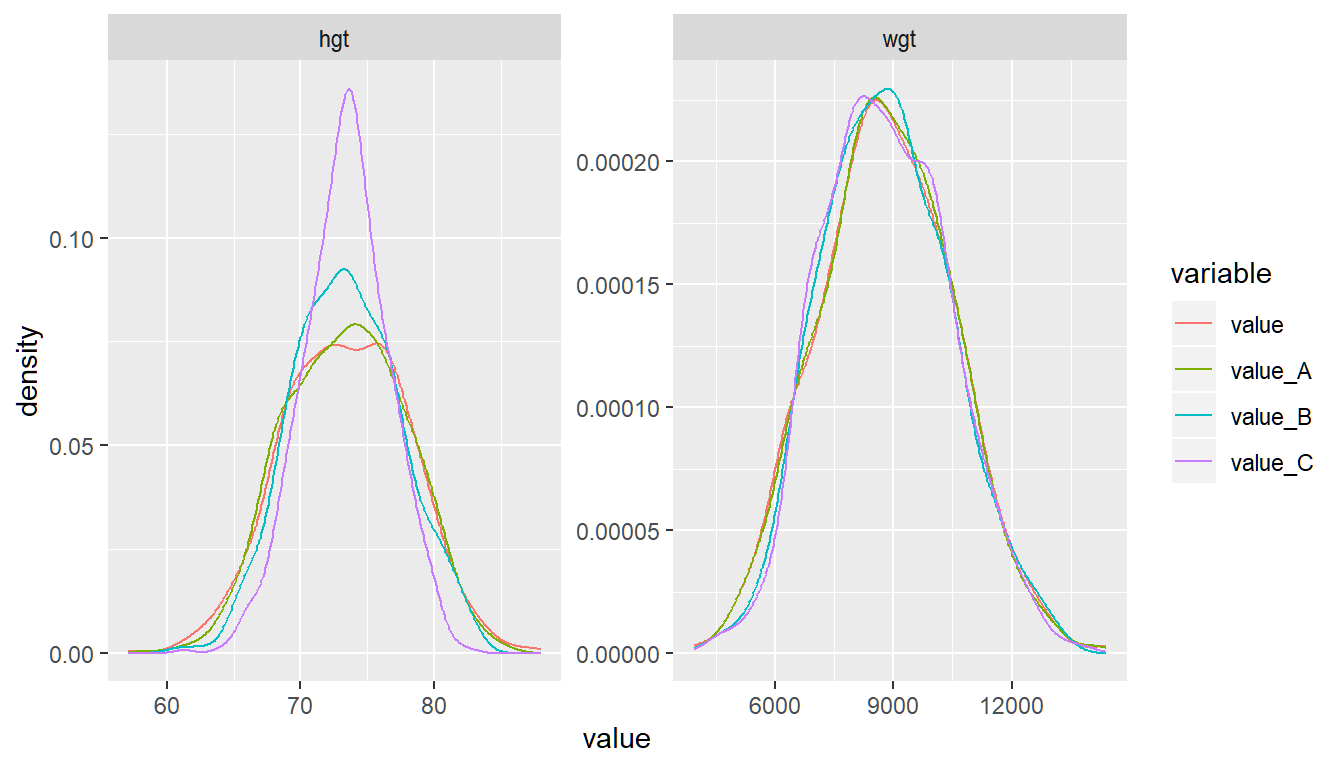
\includegraphics{Panel-Data-and-Optimization-with-R_files/figure-latex/unnamed-chunk-130-1} \end{center}

\hypertarget{example-cebu-ols}{%
\subsubsection{Example Cebu OLS}\label{example-cebu-ols}}

\begin{Shaded}
\begin{Highlighting}[]
\NormalTok{df.use <-}\StringTok{ }\NormalTok{df }\OperatorTok\StringTok{ }\KeywordTok{filter}\NormalTok{(S.country }\OperatorTok{==}\StringTok{ 'Cebu'}\NormalTok{) }\OperatorTok\StringTok{ }
\StringTok{  }\KeywordTok{filter}\NormalTok{(svymthRound }\OperatorTok\StringTok{ }\KeywordTok{c}\NormalTok{(}\DecValTok{12}\NormalTok{, }\DecValTok{18}\NormalTok{, }\DecValTok{24}\NormalTok{))}
\NormalTok{vars.z <-}\StringTok{ }\OtherTok{NULL}
\NormalTok{list.out <-}\StringTok{ }\KeywordTok{ff_lr_decompose}\NormalTok{(}
  \DataTypeTok{df=}\NormalTok{df.use, vars.y, vars.x, vars.c, vars.z, vars.other.keep,}
\NormalTok{  list.vars.tomean, list.vars.tomean.name.suffix,}
  \DataTypeTok{graph=}\OtherTok{TRUE}\NormalTok{, }\DataTypeTok{graph.nrow=}\DecValTok{1}\NormalTok{)}
\KeywordTok{options}\NormalTok{(}\DataTypeTok{repr.matrix.max.rows=}\DecValTok{10}\NormalTok{, }\DataTypeTok{repr.matrix.max.cols=}\DecValTok{50}\NormalTok{)}
\KeywordTok{head}\NormalTok{(list.out}\OperatorTok{$}\NormalTok{dfmain, }\DecValTok{10}\NormalTok{) }\OperatorTok
\StringTok{  }\KeywordTok{kable}\NormalTok{() }\OperatorTok
\StringTok{  }\KeywordTok{kable_styling_fc_wide}\NormalTok{()}
\end{Highlighting}
\end{Shaded}

\begin{table}[!h]
\centering
\resizebox{\linewidth}{!}{
\begin{tabular}{l|r|r|r|r|r|r|r|l|r|r|r|r|r|r|r|r|r|r}
\hline
S.country & vil.id & indi.id & svymthRound & prot & male & wgt0 & hgt0 & variable & value & prot\_mean & male\_mean & wgt0\_mean & hgt0\_mean & svymthRound\_mean & value\_mean & value\_A & value\_B & value\_C\\
\hline
\rowcolor{gray!6}  Cebu & 1 & 1 & 12 & 11.3 & 1 & 2043.8 & 44.2 & hgt & 70.8 & 16.95957 & 0.5263013 & 2988.773 & 49.23897 & 17.87441 & 74.99584 & 72.12171 & 72.33074 & 76.35522\\
\hline
Cebu & 1 & 2 & 12 & 5.9 & 0 & 2839.9 & 49.7 & hgt & 72.2 & 16.95957 & 0.5263013 & 2988.773 & 49.23897 & 17.87441 & 74.99584 & 72.64812 & 73.05659 & 77.08108\\
\hline
\rowcolor{gray!6}  Cebu & 1 & 2 & 18 & 0.5 & 0 & 2839.9 & 49.7 & hgt & 76.5 & 16.95957 & 0.5263013 & 2988.773 & 49.23897 & 17.87441 & 74.99584 & 76.94812 & 77.55604 & 77.47000\\
\hline
Cebu & 1 & 2 & 24 & 14.1 & 0 & 2839.9 & 49.7 & hgt & 79.2 & 16.95957 & 0.5263013 & 2988.773 & 49.23897 & 17.87441 & 74.99584 & 79.64812 & 79.75374 & 75.55718\\
\hline
\rowcolor{gray!6}  Cebu & 1 & 3 & 12 & 21.4 & 0 & 3445.6 & 51.7 & hgt & 68.0 & 16.95957 & 0.5263013 & 2988.773 & 49.23897 & 17.87441 & 74.99584 & 67.70200 & 67.53800 & 71.56248\\
\hline
Cebu & 1 & 3 & 18 & 23.6 & 0 & 3445.6 & 51.7 & hgt & 71.6 & 16.95957 & 0.5263013 & 2988.773 & 49.23897 & 17.87441 & 74.99584 & 71.30200 & 71.05674 & 70.97071\\
\hline
\rowcolor{gray!6}  Cebu & 1 & 3 & 24 & 20.6 & 0 & 3445.6 & 51.7 & hgt & 76.7 & 16.95957 & 0.5263013 & 2988.773 & 49.23897 & 17.87441 & 74.99584 & 76.40200 & 76.26754 & 72.07099\\
\hline
Cebu & 1 & 4 & 12 & 0.7 & 0 & 3090.9 & 50.2 & hgt & 69.1 & 16.95957 & 0.5263013 & 2988.773 & 49.23897 & 17.87441 & 74.99584 & 69.36159 & 69.96212 & 73.98660\\
\hline
\rowcolor{gray!6}  Cebu & 1 & 4 & 18 & 7.2 & 0 & 3090.9 & 50.2 & hgt & 74.3 & 16.95957 & 0.5263013 & 2988.773 & 49.23897 & 17.87441 & 74.99584 & 74.56159 & 74.92205 & 74.83601\\
\hline
Cebu & 1 & 4 & 24 & 10.3 & 0 & 3090.9 & 50.2 & hgt & 78.1 & 16.95957 & 0.5263013 & 2988.773 & 49.23897 & 17.87441 & 74.99584 & 78.36159 & 78.60755 & 74.41100\\
\hline
\end{tabular}}
\end{table}

\begin{Shaded}
\begin{Highlighting}[]
\KeywordTok{options}\NormalTok{(}\DataTypeTok{repr.plot.width =} \DecValTok{10}\NormalTok{, }\DataTypeTok{repr.plot.height =} \DecValTok{4}\NormalTok{)}
\NormalTok{list.out}\OperatorTok{$}\NormalTok{dfsumm }\OperatorTok
\StringTok{  }\KeywordTok{kable}\NormalTok{() }\OperatorTok
\StringTok{  }\KeywordTok{kable_styling_fc_wide}\NormalTok{()}
\end{Highlighting}
\end{Shaded}

\begin{table}[!h]
\centering
\resizebox{\linewidth}{!}{
\begin{tabular}{l|r|r|r|r|r|r|r|r|r|r}
\hline
variable & value\_var & value\_mean\_var & value\_A\_var & value\_B\_var & value\_C\_var & value\_var\_frac & value\_mean\_var\_frac & value\_A\_var\_frac & value\_B\_var\_frac & value\_C\_var\_frac\\
\hline
\rowcolor{gray!6}  hgt & 24.375 & NA & 22.561 & 21.309 & 10.001 & 1 & NA & 0.926 & 0.874 & 0.410\\
\hline
wgt & 3337460.957 & NA & 3218987.397 & 3039513.634 & 2558514.368 & 1 & NA & 0.965 & 0.911 & 0.767\\
\hline
\end{tabular}}
\end{table}

\hypertarget{example-cebu-iv}{%
\subsubsection{Example Cebu IV}\label{example-cebu-iv}}

\begin{Shaded}
\begin{Highlighting}[]
\NormalTok{df.use <-}\StringTok{ }\NormalTok{df }\OperatorTok\StringTok{ }\KeywordTok{filter}\NormalTok{(S.country }\OperatorTok{==}\StringTok{ 'Cebu'}\NormalTok{) }\OperatorTok\StringTok{ }
\StringTok{  }\KeywordTok{filter}\NormalTok{(svymthRound }\OperatorTok\StringTok{ }\KeywordTok{c}\NormalTok{(}\DecValTok{12}\NormalTok{, }\DecValTok{18}\NormalTok{, }\DecValTok{24}\NormalTok{))}
\NormalTok{vars.z <-}\StringTok{ }\KeywordTok{c}\NormalTok{(}\StringTok{'wealthIdx'}\NormalTok{)}
\NormalTok{list.out <-}\StringTok{ }\KeywordTok{ff_lr_decompose}\NormalTok{(}
  \DataTypeTok{df=}\NormalTok{df.use, vars.y, vars.x, vars.c, vars.z, vars.other.keep,}
\NormalTok{  list.vars.tomean, list.vars.tomean.name.suffix,}
  \DataTypeTok{graph=}\OtherTok{TRUE}\NormalTok{, }\DataTypeTok{graph.nrow=}\DecValTok{1}\NormalTok{)}
\end{Highlighting}
\end{Shaded}

\begin{verbatim}
## Warning: attributes are not identical across measure variables;
## they will be dropped

## Warning: attributes are not identical across measure variables;
## they will be dropped
\end{verbatim}

\begin{Shaded}
\begin{Highlighting}[]
\NormalTok{list.out}\OperatorTok{$}\NormalTok{dfsumm }\OperatorTok
\StringTok{  }\KeywordTok{kable}\NormalTok{() }\OperatorTok
\StringTok{  }\KeywordTok{kable_styling_fc_wide}\NormalTok{()}
\end{Highlighting}
\end{Shaded}

\begin{table}[!h]
\centering
\resizebox{\linewidth}{!}{
\begin{tabular}{l|r|r|r|r|r|r|r|r|r|r}
\hline
variable & value\_var & value\_mean\_var & value\_A\_var & value\_B\_var & value\_C\_var & value\_var\_frac & value\_mean\_var\_frac & value\_A\_var\_frac & value\_B\_var\_frac & value\_C\_var\_frac\\
\hline
\rowcolor{gray!6}  hgt & 24.375 & NA & 22.625 & 22.194 & 14.392 & 1 & NA & 0.928 & 0.911 & 0.590\\
\hline
wgt & 3337460.957 & NA & 3237415.252 & 3385814.742 & 3158659.340 & 1 & NA & 0.970 & 1.014 & 0.946\\
\hline
\end{tabular}}
\end{table}

\begin{Shaded}
\begin{Highlighting}[]
\KeywordTok{options}\NormalTok{(}\DataTypeTok{repr.plot.width =} \DecValTok{10}\NormalTok{, }\DataTypeTok{repr.plot.height =} \DecValTok{2}\NormalTok{)}
\NormalTok{list.out}\OperatorTok{$}\NormalTok{graph}
\end{Highlighting}
\end{Shaded}

\begin{center}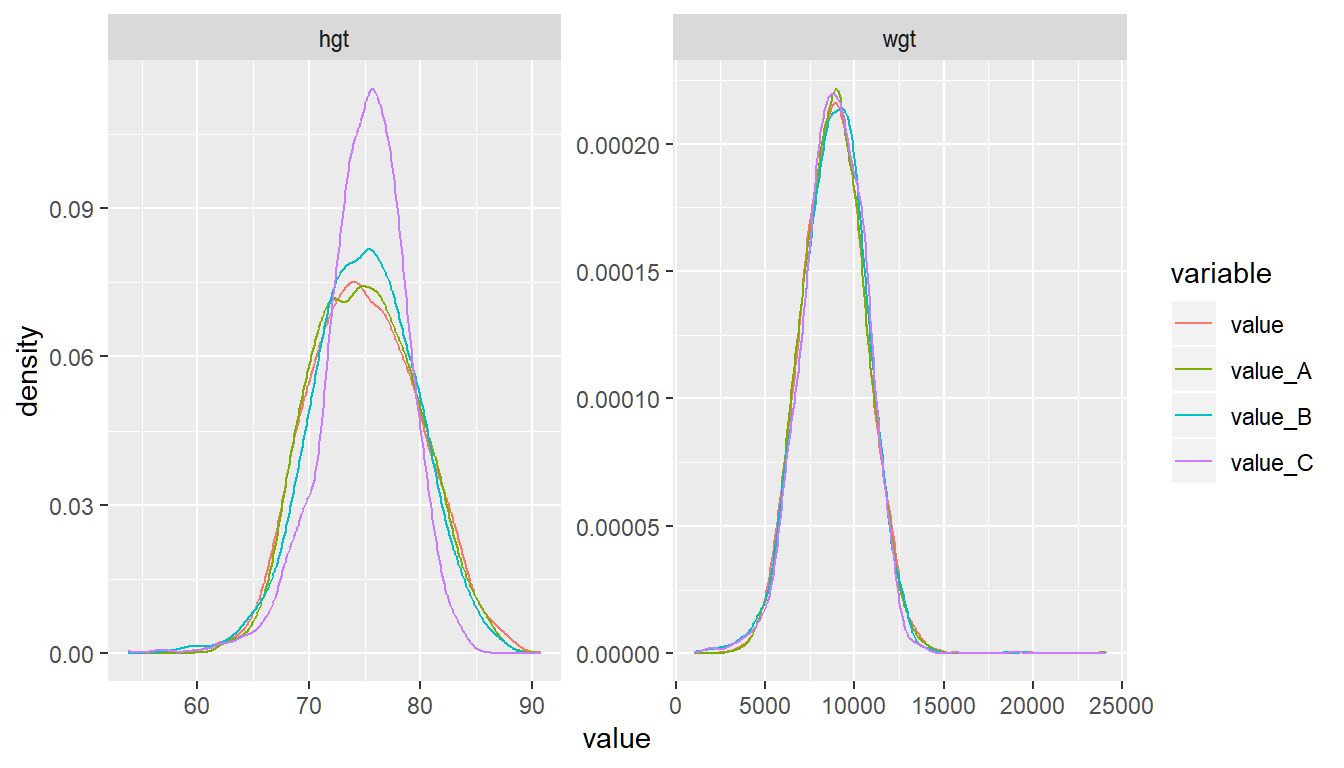
\includegraphics{Panel-Data-and-Optimization-with-R_files/figure-latex/unnamed-chunk-132-1} \end{center}

\hypertarget{examples-line-by-line-1}{%
\subsubsection{Examples Line by Line}\label{examples-line-by-line-1}}

The examples are just to test the code with different types of variables.

\begin{Shaded}
\begin{Highlighting}[]
\NormalTok{df.use <-}\StringTok{ }\NormalTok{df }\OperatorTok\StringTok{ }\KeywordTok{filter}\NormalTok{(S.country }\OperatorTok{==}\StringTok{ 'Guatemala'}\NormalTok{) }\OperatorTok\StringTok{ }
\StringTok{  }\KeywordTok{filter}\NormalTok{(svymthRound }\OperatorTok\StringTok{ }\KeywordTok{c}\NormalTok{(}\DecValTok{12}\NormalTok{, }\DecValTok{18}\NormalTok{, }\DecValTok{24}\NormalTok{))}
\KeywordTok{dim}\NormalTok{(df.use)}
\end{Highlighting}
\end{Shaded}

\begin{verbatim}
## [1] 2022   16
\end{verbatim}

Setting Up Parameters.

\begin{Shaded}
\begin{Highlighting}[]
\CommentTok{# Define Left Hand Side Variables}
\NormalTok{var.y1 <-}\StringTok{ }\KeywordTok{c}\NormalTok{(}\StringTok{'hgt'}\NormalTok{)}
\NormalTok{var.y2 <-}\StringTok{ }\KeywordTok{c}\NormalTok{(}\StringTok{'wgt'}\NormalTok{)}
\NormalTok{vars.y <-}\StringTok{ }\KeywordTok{c}\NormalTok{(var.y1, var.y2)}
\CommentTok{# Define Right Hand Side Variables}
\NormalTok{vars.x <-}\StringTok{ }\KeywordTok{c}\NormalTok{(}\StringTok{'prot'}\NormalTok{)}
\NormalTok{vars.c <-}\StringTok{ }\KeywordTok{c}\NormalTok{(}\StringTok{'male'}\NormalTok{, }\StringTok{'wgt0'}\NormalTok{, }\StringTok{'hgt0'}\NormalTok{, }\StringTok{'svymthRound'}\NormalTok{)}
\CommentTok{# vars.z <- c('p.A.prot')}
\NormalTok{vars.z <-}\StringTok{ }\KeywordTok{c}\NormalTok{(}\StringTok{'vil.id'}\NormalTok{)}
\CommentTok{# vars.z <- NULL}
\NormalTok{vars.xc <-}\StringTok{ }\KeywordTok{c}\NormalTok{(vars.x, vars.c)}

\CommentTok{# Other variables to keep}
\NormalTok{vars.other.keep <-}\StringTok{ }\KeywordTok{c}\NormalTok{(}\StringTok{'S.country'}\NormalTok{, }\StringTok{'vil.id'}\NormalTok{, }\StringTok{'indi.id'}\NormalTok{, }\StringTok{'svymthRound'}\NormalTok{)}

\CommentTok{# Decompose sequence}
\NormalTok{vars.tomean.first <-}\StringTok{ }\KeywordTok{c}\NormalTok{(}\StringTok{'male'}\NormalTok{, }\StringTok{'hgt0'}\NormalTok{)}
\NormalTok{var.tomean.first.name.suffix <-}\StringTok{ '_mh02m'}
\NormalTok{vars.tomean.second <-}\StringTok{ }\KeywordTok{c}\NormalTok{(vars.tomean.first, }\StringTok{'hgt0'}\NormalTok{, }\StringTok{'wgt0'}\NormalTok{)}
\NormalTok{var.tomean.second.name.suffix <-}\StringTok{ '_mh0me2m'}
\NormalTok{vars.tomean.third <-}\StringTok{ }\KeywordTok{c}\NormalTok{(vars.tomean.second, }\StringTok{'prot'}\NormalTok{)}
\NormalTok{var.tomean.third.name.suffix <-}\StringTok{ '_mh0mep2m'}
\NormalTok{vars.tomean.fourth <-}\StringTok{ }\KeywordTok{c}\NormalTok{(vars.tomean.third, }\StringTok{'svymthRound'}\NormalTok{)}
\NormalTok{var.tomean.fourth.name.suffix <-}\StringTok{ '_mh0mepm2m'}
\NormalTok{list.vars.tomean =}\StringTok{ }\KeywordTok{list}\NormalTok{(}
\CommentTok{#                         vars.tomean.first,}
\NormalTok{                        vars.tomean.second,}
\NormalTok{                        vars.tomean.third,}
\NormalTok{                        vars.tomean.fourth}
\NormalTok{                        )}
\NormalTok{list.vars.tomean.name.suffix <-}\StringTok{ }\KeywordTok{list}\NormalTok{(}
\CommentTok{#                                     var.tomean.first.name.suffix,}
\NormalTok{                                     var.tomean.second.name.suffix,}
\NormalTok{                                     var.tomean.third.name.suffix,}
\NormalTok{                                     var.tomean.fourth.name.suffix}
\NormalTok{                                    )}
\end{Highlighting}
\end{Shaded}

\hypertarget{obtain-regression-coefficients-from-somewhere}{%
\paragraph{Obtain Regression Coefficients from somewhere}\label{obtain-regression-coefficients-from-somewhere}}

\begin{Shaded}
\begin{Highlighting}[]
\CommentTok{# Regressions}
\CommentTok{# regf.iv from C:\textbackslash{}Users\textbackslash{}fan\textbackslash{}R4Econ\textbackslash{}linreg\textbackslash{}ivreg\textbackslash{}ivregdfrow.R}
\NormalTok{df.reg.out <-}\StringTok{ }\KeywordTok{as_tibble}\NormalTok{(}
  \KeywordTok{bind_rows}\NormalTok{(}\KeywordTok{lapply}\NormalTok{(vars.y, regf.iv,}
                   \DataTypeTok{vars.x=}\NormalTok{vars.x, }\DataTypeTok{vars.c=}\NormalTok{vars.c, }\DataTypeTok{vars.z=}\NormalTok{vars.z, }\DataTypeTok{df=}\NormalTok{df)))}
\end{Highlighting}
\end{Shaded}

\begin{verbatim}
## Warning: attributes are not identical across measure variables;
## they will be dropped

## Warning: attributes are not identical across measure variables;
## they will be dropped
\end{verbatim}

\begin{Shaded}
\begin{Highlighting}[]
\CommentTok{# Regressions}
\CommentTok{# reg1 <- regf.iv(var.y = var.y1, vars.x, vars.c, vars.z, df.use)}
\CommentTok{# reg2 <- regf.iv(var.y = var.y2, vars.x, vars.c, vars.z, df.use)}
\CommentTok{# df.reg.out <- as_tibble(bind_rows(reg1, reg2))}
\end{Highlighting}
\end{Shaded}

\begin{Shaded}
\begin{Highlighting}[]
\CommentTok{# df.reg.out }
\end{Highlighting}
\end{Shaded}

\begin{Shaded}
\begin{Highlighting}[]
\CommentTok{# Select Variables}
\NormalTok{str.esti.suffix <-}\StringTok{ '_Estimate'}
\NormalTok{arr.esti.name <-}\StringTok{ }\KeywordTok{paste0}\NormalTok{(vars.xc, str.esti.suffix)}
\NormalTok{str.outcome.name <-}\StringTok{ 'vars_var.y'}
\NormalTok{arr.columns2select <-}\StringTok{ }\KeywordTok{c}\NormalTok{(arr.esti.name, str.outcome.name)}
\NormalTok{arr.columns2select}
\end{Highlighting}
\end{Shaded}

\begin{verbatim}
## [1] "prot_Estimate"        "male_Estimate"        "wgt0_Estimate"        "hgt0_Estimate"        "svymthRound_Estimate" "vars_var.y"
\end{verbatim}

\begin{Shaded}
\begin{Highlighting}[]
\CommentTok{# Generate dataframe for coefficients}
\NormalTok{df.coef <-}\StringTok{ }\NormalTok{df.reg.out[,}\KeywordTok{c}\NormalTok{(arr.columns2select)] }\OperatorTok\StringTok{ }\KeywordTok{mutate_at}\NormalTok{(}\KeywordTok{vars}\NormalTok{(arr.esti.name), as.numeric) }\OperatorTok\StringTok{ }\KeywordTok{column_to_rownames}\NormalTok{(str.outcome.name)}
\NormalTok{df.coef }\OperatorTok
\StringTok{  }\KeywordTok{kable}\NormalTok{() }\OperatorTok
\StringTok{  }\KeywordTok{kable_styling_fc}\NormalTok{()}
\end{Highlighting}
\end{Shaded}

\begin{table}[!h]
\centering
\begin{tabular}{l|r|r|r|r|r}
\hline
  & prot\_Estimate & male\_Estimate & wgt0\_Estimate & hgt0\_Estimate & svymthRound\_Estimate\\
\hline
\rowcolor{gray!6}  hgt & -0.2714772 & 1.244735 & 0.0004430 & 0.6834853 & 1.133919\\
\hline
wgt & -59.0727542 & 489.852902 & 0.7696158 & 75.4867897 & 250.778883\\
\hline
\end{tabular}
\end{table}

\begin{Shaded}
\begin{Highlighting}[]
\KeywordTok{str}\NormalTok{(df.coef)}
\end{Highlighting}
\end{Shaded}

\begin{verbatim}
## 'data.frame':    2 obs. of  5 variables:
##  $ prot_Estimate       : num  -0.271 -59.073
##  $ male_Estimate       : num  1.24 489.85
##  $ wgt0_Estimate       : num  0.000443 0.769616
##  $ hgt0_Estimate       : num  0.683 75.487
##  $ svymthRound_Estimate: num  1.13 250.78
\end{verbatim}

\hypertarget{decomposition-step-1}{%
\paragraph{Decomposition Step 1}\label{decomposition-step-1}}

\begin{Shaded}
\begin{Highlighting}[]
\CommentTok{# Decomposition Step 1: gather}
\NormalTok{df.decompose_step1 <-}\StringTok{ }\NormalTok{df.use }\OperatorTok
\StringTok{                        }\KeywordTok{filter}\NormalTok{(svymthRound }\OperatorTok\StringTok{ }\KeywordTok{c}\NormalTok{(}\DecValTok{12}\NormalTok{, }\DecValTok{18}\NormalTok{, }\DecValTok{24}\NormalTok{)) }\OperatorTok
\StringTok{                        }\KeywordTok{select}\NormalTok{(}\KeywordTok{one_of}\NormalTok{(}\KeywordTok{c}\NormalTok{(vars.other.keep, vars.xc, vars.y))) }\OperatorTok
\StringTok{                        }\KeywordTok{drop_na}\NormalTok{() }\OperatorTok
\StringTok{                        }\KeywordTok{gather}\NormalTok{(variable, value, }\OperatorTok{-}\KeywordTok{one_of}\NormalTok{(}\KeywordTok{c}\NormalTok{(vars.other.keep, vars.xc)))}
\KeywordTok{options}\NormalTok{(}\DataTypeTok{repr.matrix.max.rows=}\DecValTok{20}\NormalTok{, }\DataTypeTok{repr.matrix.max.cols=}\DecValTok{20}\NormalTok{)}
\KeywordTok{dim}\NormalTok{(df.decompose_step1)}
\end{Highlighting}
\end{Shaded}

\begin{verbatim}
## [1] 1382   10
\end{verbatim}

\begin{Shaded}
\begin{Highlighting}[]
\KeywordTok{head}\NormalTok{(df.decompose_step1, }\DecValTok{10}\NormalTok{) }\OperatorTok
\StringTok{  }\KeywordTok{kable}\NormalTok{() }\OperatorTok
\StringTok{  }\KeywordTok{kable_styling_fc}\NormalTok{()}
\end{Highlighting}
\end{Shaded}

\begin{table}[!h]
\centering
\begin{tabular}{l|r|r|r|r|r|r|r|l|r}
\hline
S.country & vil.id & indi.id & svymthRound & prot & male & wgt0 & hgt0 & variable & value\\
\hline
\rowcolor{gray!6}  Guatemala & 3 & 1352 & 18 & 13.3 & 1 & 2545.2 & 47.4 & hgt & 70.2\\
\hline
Guatemala & 3 & 1352 & 24 & 46.3 & 1 & 2545.2 & 47.4 & hgt & 75.8\\
\hline
\rowcolor{gray!6}  Guatemala & 3 & 1354 & 12 & 1.0 & 1 & 3634.3 & 51.2 & hgt & 66.3\\
\hline
Guatemala & 3 & 1354 & 18 & 9.8 & 1 & 3634.3 & 51.2 & hgt & 69.2\\
\hline
\rowcolor{gray!6}  Guatemala & 3 & 1354 & 24 & 15.4 & 1 & 3634.3 & 51.2 & hgt & 75.3\\
\hline
Guatemala & 3 & 1356 & 12 & 8.6 & 1 & 3911.8 & 51.9 & hgt & 68.1\\
\hline
\rowcolor{gray!6}  Guatemala & 3 & 1356 & 18 & 17.8 & 1 & 3911.8 & 51.9 & hgt & 74.1\\
\hline
Guatemala & 3 & 1356 & 24 & 30.5 & 1 & 3911.8 & 51.9 & hgt & 77.1\\
\hline
\rowcolor{gray!6}  Guatemala & 3 & 1357 & 12 & 1.0 & 1 & 3791.4 & 52.6 & hgt & 71.5\\
\hline
Guatemala & 3 & 1357 & 18 & 12.7 & 1 & 3791.4 & 52.6 & hgt & 77.8\\
\hline
\end{tabular}
\end{table}

\hypertarget{decomposition-step-2}{%
\paragraph{Decomposition Step 2}\label{decomposition-step-2}}

\begin{Shaded}
\begin{Highlighting}[]
\CommentTok{# Decomposition Step 2: mutate_at(vars, funs(mean = mean(.)))}
\CommentTok{# the xc averaging could have taken place earlier, no difference in mean across variables}
\NormalTok{df.decompose_step2 <-}\StringTok{ }\NormalTok{df.decompose_step1 }\OperatorTok
\StringTok{                        }\KeywordTok{group_by}\NormalTok{(variable) }\OperatorTok
\StringTok{                        }\KeywordTok{mutate_at}\NormalTok{(}\KeywordTok{vars}\NormalTok{(}\KeywordTok{c}\NormalTok{(vars.xc, }\StringTok{'value'}\NormalTok{)), }\KeywordTok{funs}\NormalTok{(}\DataTypeTok{mean =} \KeywordTok{mean}\NormalTok{(.))) }\OperatorTok
\StringTok{                        }\KeywordTok{ungroup}\NormalTok{()}

\KeywordTok{options}\NormalTok{(}\DataTypeTok{repr.matrix.max.rows=}\DecValTok{20}\NormalTok{, }\DataTypeTok{repr.matrix.max.cols=}\DecValTok{20}\NormalTok{)}
\KeywordTok{dim}\NormalTok{(df.decompose_step2)}
\end{Highlighting}
\end{Shaded}

\begin{verbatim}
## [1] 1382   16
\end{verbatim}

\begin{Shaded}
\begin{Highlighting}[]
\KeywordTok{head}\NormalTok{(df.decompose_step2,}\DecValTok{10}\NormalTok{) }\OperatorTok
\StringTok{  }\KeywordTok{kable}\NormalTok{() }\OperatorTok
\StringTok{  }\KeywordTok{kable_styling_fc_wide}\NormalTok{()}
\end{Highlighting}
\end{Shaded}

\begin{table}[!h]
\centering
\resizebox{\linewidth}{!}{
\begin{tabular}{l|r|r|r|r|r|r|r|l|r|r|r|r|r|r|r}
\hline
S.country & vil.id & indi.id & svymthRound & prot & male & wgt0 & hgt0 & variable & value & prot\_mean & male\_mean & wgt0\_mean & hgt0\_mean & svymthRound\_mean & value\_mean\\
\hline
\rowcolor{gray!6}  Guatemala & 3 & 1352 & 18 & 13.3 & 1 & 2545.2 & 47.4 & hgt & 70.2 & 20.64819 & 0.5499276 & 3312.297 & 49.75137 & 18.42547 & 73.41216\\
\hline
Guatemala & 3 & 1352 & 24 & 46.3 & 1 & 2545.2 & 47.4 & hgt & 75.8 & 20.64819 & 0.5499276 & 3312.297 & 49.75137 & 18.42547 & 73.41216\\
\hline
\rowcolor{gray!6}  Guatemala & 3 & 1354 & 12 & 1.0 & 1 & 3634.3 & 51.2 & hgt & 66.3 & 20.64819 & 0.5499276 & 3312.297 & 49.75137 & 18.42547 & 73.41216\\
\hline
Guatemala & 3 & 1354 & 18 & 9.8 & 1 & 3634.3 & 51.2 & hgt & 69.2 & 20.64819 & 0.5499276 & 3312.297 & 49.75137 & 18.42547 & 73.41216\\
\hline
\rowcolor{gray!6}  Guatemala & 3 & 1354 & 24 & 15.4 & 1 & 3634.3 & 51.2 & hgt & 75.3 & 20.64819 & 0.5499276 & 3312.297 & 49.75137 & 18.42547 & 73.41216\\
\hline
Guatemala & 3 & 1356 & 12 & 8.6 & 1 & 3911.8 & 51.9 & hgt & 68.1 & 20.64819 & 0.5499276 & 3312.297 & 49.75137 & 18.42547 & 73.41216\\
\hline
\rowcolor{gray!6}  Guatemala & 3 & 1356 & 18 & 17.8 & 1 & 3911.8 & 51.9 & hgt & 74.1 & 20.64819 & 0.5499276 & 3312.297 & 49.75137 & 18.42547 & 73.41216\\
\hline
Guatemala & 3 & 1356 & 24 & 30.5 & 1 & 3911.8 & 51.9 & hgt & 77.1 & 20.64819 & 0.5499276 & 3312.297 & 49.75137 & 18.42547 & 73.41216\\
\hline
\rowcolor{gray!6}  Guatemala & 3 & 1357 & 12 & 1.0 & 1 & 3791.4 & 52.6 & hgt & 71.5 & 20.64819 & 0.5499276 & 3312.297 & 49.75137 & 18.42547 & 73.41216\\
\hline
Guatemala & 3 & 1357 & 18 & 12.7 & 1 & 3791.4 & 52.6 & hgt & 77.8 & 20.64819 & 0.5499276 & 3312.297 & 49.75137 & 18.42547 & 73.41216\\
\hline
\end{tabular}}
\end{table}

\hypertarget{decomposition-step-3-non-loop}{%
\paragraph{Decomposition Step 3 Non-Loop}\label{decomposition-step-3-non-loop}}

\begin{Shaded}
\begin{Highlighting}[]
\NormalTok{ff_lr_decompose_valadj <-}\StringTok{ }\ControlFlowTok{function}\NormalTok{(df, df.coef, vars.tomean, str.esti.suffix) \{}
\NormalTok{    new_value <-}\StringTok{ }\NormalTok{(df}\OperatorTok{$}\NormalTok{value }\OperatorTok{+}
\StringTok{                  }\KeywordTok{rowSums}\NormalTok{((df[}\KeywordTok{paste0}\NormalTok{(vars.tomean, }\StringTok{'_mean'}\NormalTok{)] }\OperatorTok{-}\StringTok{ }\NormalTok{df[vars.tomean])}
                          \OperatorTok{*}\NormalTok{df.coef[df}\OperatorTok{$}\NormalTok{variable, }\KeywordTok{paste0}\NormalTok{(vars.tomean, str.esti.suffix)]))}
    \KeywordTok{return}\NormalTok{(new_value)}
\NormalTok{\}}

\CommentTok{# # Decomposition Step 3: mutate_at(vars, funs(mean = mean(.)))}
\CommentTok{# var.decomp.one <- (paste0('value', list.vars.tomean.name.suffix[[1]]))}
\CommentTok{# var.decomp.two <- (paste0('value', list.vars.tomean.name.suffix[[2]]))}
\CommentTok{# var.decomp.thr <- (paste0('value', list.vars.tomean.name.suffix[[3]]))}
\CommentTok{# df.decompose_step3 <- df.decompose_step2 %>%}
\CommentTok{#                         mutate((!!var.decomp.one) := f_decompose_here(., df.coef, list.vars.tomean[[1]], str.esti.suffix),}
\CommentTok{#                                (!!var.decomp.two) := f_decompose_here(., df.coef, list.vars.tomean[[2]], str.esti.suffix),}
\CommentTok{#                                (!!var.decomp.thr) := f_decompose_here(., df.coef, list.vars.tomean[[3]], str.esti.suffix))}

\CommentTok{# options(repr.matrix.max.rows=10, repr.matrix.max.cols=20)}
\CommentTok{# dim(df.decompose_step3)}
\CommentTok{# df.decompose_step3}
\end{Highlighting}
\end{Shaded}

\hypertarget{decomposition-step-3-with-loop}{%
\paragraph{Decomposition Step 3 With Loop}\label{decomposition-step-3-with-loop}}

\begin{Shaded}
\begin{Highlighting}[]
\NormalTok{df.decompose_step3 <-}\StringTok{ }\NormalTok{df.decompose_step2}
\ControlFlowTok{for}\NormalTok{ (i }\ControlFlowTok{in} \DecValTok{1}\OperatorTok{:}\KeywordTok{length}\NormalTok{(list.vars.tomean)) \{}
\NormalTok{    var.decomp.cur <-}\StringTok{ }\NormalTok{(}\KeywordTok{paste0}\NormalTok{(}\StringTok{'value'}\NormalTok{, list.vars.tomean.name.suffix[[i]]))}
\NormalTok{    vars.tomean <-}\StringTok{ }\NormalTok{list.vars.tomean[[i]]}
\NormalTok{    var.decomp.cur}
\NormalTok{    df.decompose_step3 <-}\StringTok{ }\NormalTok{df.decompose_step3 }\OperatorTok\StringTok{ }
\StringTok{      }\KeywordTok{mutate}\NormalTok{((}\OperatorTok{!!}\NormalTok{var.decomp.cur) }\OperatorTok{:}\ErrorTok{=}\StringTok{ }
\StringTok{               }\KeywordTok{ff_lr_decompose_valadj}\NormalTok{(., df.coef, vars.tomean, str.esti.suffix))}

\NormalTok{\}}
\KeywordTok{options}\NormalTok{(}\DataTypeTok{repr.matrix.max.rows=}\DecValTok{10}\NormalTok{, }\DataTypeTok{repr.matrix.max.cols=}\DecValTok{20}\NormalTok{)}
\KeywordTok{dim}\NormalTok{(df.decompose_step3)}
\end{Highlighting}
\end{Shaded}

\begin{verbatim}
## [1] 1382   19
\end{verbatim}

\begin{Shaded}
\begin{Highlighting}[]
\KeywordTok{head}\NormalTok{(df.decompose_step3, }\DecValTok{10}\NormalTok{) }\OperatorTok
\StringTok{  }\KeywordTok{kable}\NormalTok{() }\OperatorTok
\StringTok{  }\KeywordTok{kable_styling_fc_wide}\NormalTok{()}
\end{Highlighting}
\end{Shaded}

\begin{table}[!h]
\centering
\resizebox{\linewidth}{!}{
\begin{tabular}{l|r|r|r|r|r|r|r|l|r|r|r|r|r|r|r|r|r|r}
\hline
S.country & vil.id & indi.id & svymthRound & prot & male & wgt0 & hgt0 & variable & value & prot\_mean & male\_mean & wgt0\_mean & hgt0\_mean & svymthRound\_mean & value\_mean & value\_mh0me2m & value\_mh0mep2m & value\_mh0mepm2m\\
\hline
\rowcolor{gray!6}  Guatemala & 3 & 1352 & 18 & 13.3 & 1 & 2545.2 & 47.4 & hgt & 70.2 & 20.64819 & 0.5499276 & 3312.297 & 49.75137 & 18.42547 & 73.41216 & 73.19390 & 71.19903 & 71.68148\\
\hline
Guatemala & 3 & 1352 & 24 & 46.3 & 1 & 2545.2 & 47.4 & hgt & 75.8 & 20.64819 & 0.5499276 & 3312.297 & 49.75137 & 18.42547 & 73.41216 & 78.79390 & 85.75778 & 79.43671\\
\hline
\rowcolor{gray!6}  Guatemala & 3 & 1354 & 12 & 1.0 & 1 & 3634.3 & 51.2 & hgt & 66.3 & 20.64819 & 0.5499276 & 3312.297 & 49.75137 & 18.42547 & 73.41216 & 63.61689 & 58.28285 & 65.56882\\
\hline
Guatemala & 3 & 1354 & 18 & 9.8 & 1 & 3634.3 & 51.2 & hgt & 69.2 & 20.64819 & 0.5499276 & 3312.297 & 49.75137 & 18.42547 & 73.41216 & 66.51689 & 63.57185 & 64.05430\\
\hline
\rowcolor{gray!6}  Guatemala & 3 & 1354 & 24 & 15.4 & 1 & 3634.3 & 51.2 & hgt & 75.3 & 20.64819 & 0.5499276 & 3312.297 & 49.75137 & 18.42547 & 73.41216 & 72.61689 & 71.19213 & 64.87106\\
\hline
Guatemala & 3 & 1356 & 12 & 8.6 & 1 & 3911.8 & 51.9 & hgt & 68.1 & 20.64819 & 0.5499276 & 3312.297 & 49.75137 & 18.42547 & 73.41216 & 64.33707 & 61.06626 & 68.35222\\
\hline
\rowcolor{gray!6}  Guatemala & 3 & 1356 & 18 & 17.8 & 1 & 3911.8 & 51.9 & hgt & 74.1 & 20.64819 & 0.5499276 & 3312.297 & 49.75137 & 18.42547 & 73.41216 & 70.33707 & 69.56385 & 70.04630\\
\hline
Guatemala & 3 & 1356 & 24 & 30.5 & 1 & 3911.8 & 51.9 & hgt & 77.1 & 20.64819 & 0.5499276 & 3312.297 & 49.75137 & 18.42547 & 73.41216 & 73.33707 & 76.01161 & 69.69055\\
\hline
\rowcolor{gray!6}  Guatemala & 3 & 1357 & 12 & 1.0 & 1 & 3791.4 & 52.6 & hgt & 71.5 & 20.64819 & 0.5499276 & 3312.297 & 49.75137 & 18.42547 & 73.41216 & 66.83353 & 61.49949 & 68.78545\\
\hline
Guatemala & 3 & 1357 & 18 & 12.7 & 1 & 3791.4 & 52.6 & hgt & 77.8 & 20.64819 & 0.5499276 & 3312.297 & 49.75137 & 18.42547 & 73.41216 & 73.13353 & 70.97578 & 71.45823\\
\hline
\end{tabular}}
\end{table}

\hypertarget{decomposition-step-4-variance}{%
\paragraph{Decomposition Step 4 Variance}\label{decomposition-step-4-variance}}

\begin{Shaded}
\begin{Highlighting}[]
\NormalTok{df.decompose_step3 }\OperatorTok
\StringTok{        }\KeywordTok{select}\NormalTok{(variable, }\KeywordTok{contains}\NormalTok{(}\StringTok{'value'}\NormalTok{)) }\OperatorTok
\StringTok{        }\KeywordTok{group_by}\NormalTok{(variable) }\OperatorTok
\StringTok{        }\KeywordTok{summarize_all}\NormalTok{(}\KeywordTok{funs}\NormalTok{(}\DataTypeTok{mean =}\NormalTok{ mean, }\DataTypeTok{var =}\NormalTok{ var)) }\OperatorTok
\StringTok{        }\KeywordTok{select}\NormalTok{(}\KeywordTok{matches}\NormalTok{(}\StringTok{'value'}\NormalTok{)) }\OperatorTok\StringTok{ }\KeywordTok{select}\NormalTok{(}\KeywordTok{ends_with}\NormalTok{(}\StringTok{"_var"}\NormalTok{)) }\OperatorTok
\StringTok{        }\KeywordTok{mutate_if}\NormalTok{(is.numeric, }\KeywordTok{funs}\NormalTok{( }\DataTypeTok{frac =}\NormalTok{ (.}\OperatorTok{/}\NormalTok{value_var))) }\OperatorTok
\StringTok{        }\KeywordTok{mutate_if}\NormalTok{(is.numeric, round, }\DecValTok{3}\NormalTok{) }\OperatorTok
\StringTok{  }\KeywordTok{kable}\NormalTok{() }\OperatorTok
\StringTok{  }\KeywordTok{kable_styling_fc}\NormalTok{()}
\end{Highlighting}
\end{Shaded}

\begin{table}[!h]
\centering
\begin{tabular}{r|r|r|r|r|r|r|r|r|r}
\hline
value\_var & value\_mean\_var & value\_mh0me2m\_var & value\_mh0mep2m\_var & value\_mh0mepm2m\_var & value\_var\_frac & value\_mean\_var\_frac & value\_mh0me2m\_var\_frac & value\_mh0mep2m\_var\_frac & value\_mh0mepm2m\_var\_frac\\
\hline
\rowcolor{gray!6}  21.864 & NA & 25.35 & 49.047 & 23.06 & 1 & NA & 1.159 & 2.243 & 1.055\\
\hline
2965693.245 & NA & 2949187.64 & 4192769.518 & 3147506.60 & 1 & NA & 0.994 & 1.414 & 1.061\\
\hline
\end{tabular}
\end{table}

\hypertarget{graphical-results}{%
\paragraph{Graphical Results}\label{graphical-results}}

Graphically, difficult to pick up exact differences in variance, a 50 percent reduction in variance visually does not look like 50 percent. Intuitively, we are kind of seeing standard deviation, not variance on the graph if we think abou the x-scale.

\begin{Shaded}
\begin{Highlighting}[]
\KeywordTok{head}\NormalTok{(df.decompose_step3 }\OperatorTok
\StringTok{    }\KeywordTok{select}\NormalTok{(variable, }\KeywordTok{contains}\NormalTok{(}\StringTok{'value'}\NormalTok{), }\OperatorTok{-}\NormalTok{value_mean), }\DecValTok{10}\NormalTok{) }\OperatorTok
\StringTok{  }\KeywordTok{kable}\NormalTok{() }\OperatorTok
\StringTok{  }\KeywordTok{kable_styling_fc_wide}\NormalTok{()}
\end{Highlighting}
\end{Shaded}

\begin{table}[!h]
\centering
\resizebox{\linewidth}{!}{
\begin{tabular}{l|r|r|r|r}
\hline
variable & value & value\_mh0me2m & value\_mh0mep2m & value\_mh0mepm2m\\
\hline
\rowcolor{gray!6}  hgt & 70.2 & 73.19390 & 71.19903 & 71.68148\\
\hline
hgt & 75.8 & 78.79390 & 85.75778 & 79.43671\\
\hline
\rowcolor{gray!6}  hgt & 66.3 & 63.61689 & 58.28285 & 65.56882\\
\hline
hgt & 69.2 & 66.51689 & 63.57185 & 64.05430\\
\hline
\rowcolor{gray!6}  hgt & 75.3 & 72.61689 & 71.19213 & 64.87106\\
\hline
hgt & 68.1 & 64.33707 & 61.06626 & 68.35222\\
\hline
\rowcolor{gray!6}  hgt & 74.1 & 70.33707 & 69.56385 & 70.04630\\
\hline
hgt & 77.1 & 73.33707 & 76.01161 & 69.69055\\
\hline
\rowcolor{gray!6}  hgt & 71.5 & 66.83353 & 61.49949 & 68.78545\\
\hline
hgt & 77.8 & 73.13353 & 70.97578 & 71.45823\\
\hline
\end{tabular}}
\end{table}

\begin{Shaded}
\begin{Highlighting}[]
\KeywordTok{options}\NormalTok{(}\DataTypeTok{repr.plot.width =} \DecValTok{10}\NormalTok{, }\DataTypeTok{repr.plot.height =} \DecValTok{4}\NormalTok{)}
\NormalTok{df.decompose_step3 }\OperatorTok
\StringTok{    }\KeywordTok{select}\NormalTok{(variable, }\KeywordTok{contains}\NormalTok{(}\StringTok{'value'}\NormalTok{), }\OperatorTok{-}\NormalTok{value_mean) }\OperatorTok
\StringTok{    }\KeywordTok{rename}\NormalTok{(}\DataTypeTok{outcome =}\NormalTok{ variable) }\OperatorTok
\StringTok{    }\KeywordTok{gather}\NormalTok{(variable, value, }\OperatorTok{-}\NormalTok{outcome) }\OperatorTok
\StringTok{    }\KeywordTok{ggplot}\NormalTok{(}\KeywordTok{aes}\NormalTok{(}\DataTypeTok{x=}\NormalTok{value, }\DataTypeTok{color =}\NormalTok{ variable, }\DataTypeTok{fill =}\NormalTok{ variable)) }\OperatorTok{+}
\StringTok{        }\KeywordTok{geom_line}\NormalTok{(}\DataTypeTok{stat =} \StringTok{"density"}\NormalTok{) }\OperatorTok{+}
\StringTok{        }\KeywordTok{facet_wrap}\NormalTok{(}\OperatorTok{~}\StringTok{ }\NormalTok{outcome, }\DataTypeTok{scales=}\StringTok{'free'}\NormalTok{, }\DataTypeTok{nrow=}\DecValTok{2}\NormalTok{)}
\end{Highlighting}
\end{Shaded}

\begin{center}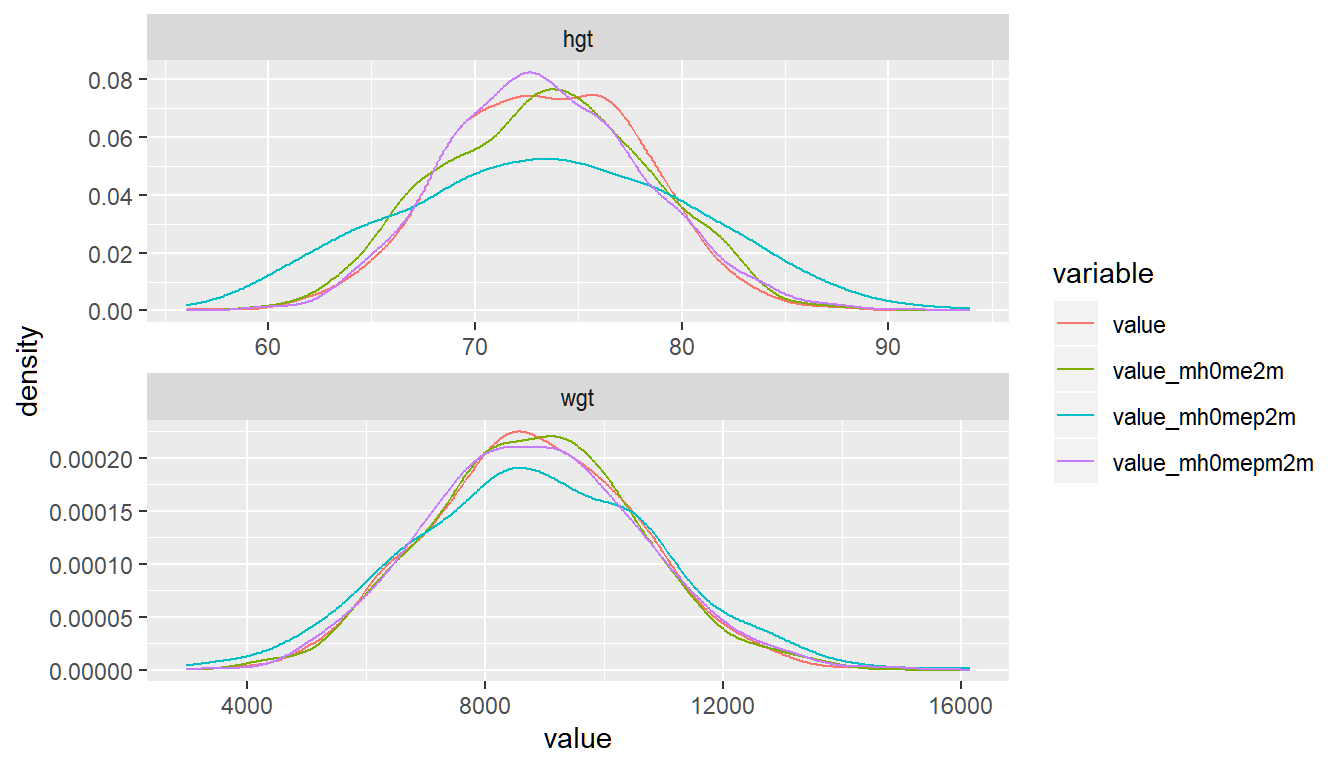
\includegraphics{Panel-Data-and-Optimization-with-R_files/figure-latex/unnamed-chunk-145-1} \end{center}

\hypertarget{additional-decomposition-testings}{%
\subsubsection{Additional Decomposition Testings}\label{additional-decomposition-testings}}

\begin{Shaded}
\begin{Highlighting}[]
\KeywordTok{head}\NormalTok{(df.decompose_step2[vars.tomean.first],}\DecValTok{3}\NormalTok{)}
\end{Highlighting}
\end{Shaded}

\begin{verbatim}
## # A tibble: 3 x 2
##    male  hgt0
##   <dbl> <dbl>
## 1     1  47.4
## 2     1  47.4
## 3     1  51.2
\end{verbatim}

\begin{Shaded}
\begin{Highlighting}[]
\KeywordTok{head}\NormalTok{(df.decompose_step2[}\KeywordTok{paste0}\NormalTok{(vars.tomean.first, }\StringTok{'_mean'}\NormalTok{)], }\DecValTok{3}\NormalTok{)}
\end{Highlighting}
\end{Shaded}

\begin{verbatim}
## # A tibble: 3 x 2
##   male_mean hgt0_mean
##       <dbl>     <dbl>
## 1     0.550      49.8
## 2     0.550      49.8
## 3     0.550      49.8
\end{verbatim}

\begin{Shaded}
\begin{Highlighting}[]
\KeywordTok{head}\NormalTok{(df.coef[df.decompose_step2}\OperatorTok{$}\NormalTok{variable, }
             \KeywordTok{paste0}\NormalTok{(vars.tomean.first, str.esti.suffix)], }\DecValTok{3}\NormalTok{)}
\end{Highlighting}
\end{Shaded}

\begin{verbatim}
##       male_Estimate hgt0_Estimate
## hgt        1.244735     0.6834853
## hgt.1      1.244735     0.6834853
## hgt.2      1.244735     0.6834853
\end{verbatim}

\begin{Shaded}
\begin{Highlighting}[]
\NormalTok{df.decompose.tomean.first <-}\StringTok{ }\NormalTok{df.decompose_step2 }\OperatorTok
\StringTok{    }\KeywordTok{mutate}\NormalTok{(}\DataTypeTok{pred_new =}\NormalTok{ df.decompose_step2}\OperatorTok{$}\NormalTok{value }\OperatorTok{+}
\StringTok{        }\KeywordTok{rowSums}\NormalTok{((df.decompose_step2[}\KeywordTok{paste0}\NormalTok{(vars.tomean.first, }\StringTok{'_mean'}\NormalTok{)] }
                 \OperatorTok{-}\StringTok{ }\NormalTok{df.decompose_step2[vars.tomean.first])}
            \OperatorTok{*}\NormalTok{df.coef[df.decompose_step2}\OperatorTok{$}\NormalTok{variable, }
                     \KeywordTok{paste0}\NormalTok{(vars.tomean.first, str.esti.suffix)])) }\OperatorTok
\StringTok{        }\KeywordTok{select}\NormalTok{(variable, value, pred_new)}
\KeywordTok{head}\NormalTok{(df.decompose.tomean.first, }\DecValTok{10}\NormalTok{)}
\end{Highlighting}
\end{Shaded}

\begin{verbatim}
## # A tibble: 10 x 3
##    variable value pred_new
##    <chr>    <dbl>    <dbl>
##  1 hgt       70.2     71.2
##  2 hgt       75.8     76.8
##  3 hgt       66.3     64.7
##  4 hgt       69.2     67.6
##  5 hgt       75.3     73.7
##  6 hgt       68.1     66.1
##  7 hgt       74.1     72.1
##  8 hgt       77.1     75.1
##  9 hgt       71.5     69.0
## 10 hgt       77.8     75.3
\end{verbatim}

\begin{Shaded}
\begin{Highlighting}[]
\NormalTok{df.decompose.tomean.first }\OperatorTok
\StringTok{        }\KeywordTok{group_by}\NormalTok{(variable) }\OperatorTok
\StringTok{        }\KeywordTok{summarize_all}\NormalTok{(}\KeywordTok{funs}\NormalTok{(}\DataTypeTok{mean =}\NormalTok{ mean, }\DataTypeTok{sd =}\NormalTok{ sd))  }\OperatorTok
\StringTok{  }\KeywordTok{kable}\NormalTok{() }\OperatorTok
\StringTok{  }\KeywordTok{kable_styling_fc}\NormalTok{()}
\end{Highlighting}
\end{Shaded}

\begin{table}[!h]
\centering
\begin{tabular}{l|r|r|r|r}
\hline
variable & value\_mean & pred\_new\_mean & value\_sd & pred\_new\_sd\\
\hline
\rowcolor{gray!6}  hgt & 73.41216 & 73.41216 & 4.675867 & 4.534947\\
\hline
wgt & 8807.87656 & 8807.87656 & 1722.118824 & 1695.221845\\
\hline
\end{tabular}
\end{table}

Note the r-square from regression above matches up with the 1 - ratio below. This is the proper decomposition method that is equivalent to r2.

\begin{Shaded}
\begin{Highlighting}[]
\NormalTok{df.decompose_step2 }\OperatorTok
\StringTok{    }\KeywordTok{mutate}\NormalTok{(}\DataTypeTok{pred_new =}\NormalTok{ df.decompose_step2}\OperatorTok{$}\NormalTok{value }\OperatorTok{+}
\StringTok{        }\KeywordTok{rowSums}\NormalTok{((df.decompose_step2[}\KeywordTok{paste0}\NormalTok{(vars.tomean.second, }\StringTok{'_mean'}\NormalTok{)] }
                 \OperatorTok{-}\StringTok{ }\NormalTok{df.decompose_step2[vars.tomean.second])}
            \OperatorTok{*}\NormalTok{df.coef[df.decompose_step2}\OperatorTok{$}\NormalTok{variable, }
                     \KeywordTok{paste0}\NormalTok{(vars.tomean.second, str.esti.suffix)])) }\OperatorTok
\StringTok{        }\KeywordTok{select}\NormalTok{(variable, value, pred_new) }\OperatorTok
\StringTok{        }\KeywordTok{group_by}\NormalTok{(variable) }\OperatorTok
\StringTok{        }\KeywordTok{summarize_all}\NormalTok{(}\KeywordTok{funs}\NormalTok{(}\DataTypeTok{mean =}\NormalTok{ mean, }\DataTypeTok{var =}\NormalTok{ var)) }\OperatorTok
\StringTok{        }\KeywordTok{mutate}\NormalTok{(}\DataTypeTok{ratio =}\NormalTok{ (pred_new_var}\OperatorTok{/}\NormalTok{value_var))  }\OperatorTok
\StringTok{  }\KeywordTok{kable}\NormalTok{() }\OperatorTok
\StringTok{  }\KeywordTok{kable_styling_fc}\NormalTok{()}
\end{Highlighting}
\end{Shaded}

\begin{table}[!h]
\centering
\begin{tabular}{l|r|r|r|r|r}
\hline
variable & value\_mean & pred\_new\_mean & value\_var & pred\_new\_var & ratio\\
\hline
\rowcolor{gray!6}  hgt & 73.41216 & 73.41216 & 2.186374e+01 & 25.3504 & 1.1594724\\
\hline
wgt & 8807.87656 & 8807.87656 & 2.965693e+06 & 2949187.6357 & 0.9944345\\
\hline
\end{tabular}
\end{table}

\hypertarget{nonlinear-regression}{%
\chapter{Nonlinear Regression}\label{nonlinear-regression}}

\hypertarget{logit-regression}{%
\section{Logit Regression}\label{logit-regression}}

\hypertarget{binary-logit}{%
\subsection{Binary Logit}\label{binary-logit}}

\begin{quote}
Go back to \href{http://fanwangecon.github.io/}{fan}'s \href{https://fanwangecon.github.io/REconTools/}{REconTools} Package, \href{https://fanwangecon.github.io/R4Econ/}{R4Econ} Repository (\href{https://fanwangecon.github.io/R4Econ/bookdown}{bookdown site}), or \href{https://fanwangecon.github.io/Stat4Econ/}{Intro Stats with R} Repository.
\end{quote}

\emph{Data Preparation}

\begin{Shaded}
\begin{Highlighting}[]
\NormalTok{df_mtcars <-}\StringTok{ }\NormalTok{mtcars}

\CommentTok{# X-variables to use on RHS}
\NormalTok{ls_st_xs <-}\StringTok{ }\KeywordTok{c}\NormalTok{(}\StringTok{'mpg'}\NormalTok{, }\StringTok{'qsec'}\NormalTok{)}
\NormalTok{ls_st_xs <-}\StringTok{ }\KeywordTok{c}\NormalTok{(}\StringTok{'mpg'}\NormalTok{)}
\NormalTok{ls_st_xs <-}\StringTok{ }\KeywordTok{c}\NormalTok{(}\StringTok{'qsec'}\NormalTok{)}
\NormalTok{ls_st_xs <-}\StringTok{ }\KeywordTok{c}\NormalTok{(}\StringTok{'wt'}\NormalTok{)}
\NormalTok{ls_st_xs <-}\StringTok{ }\KeywordTok{c}\NormalTok{(}\StringTok{'mpg'}\NormalTok{, }\StringTok{'wt'}\NormalTok{, }\StringTok{'vs'}\NormalTok{)}

\NormalTok{svr_binary <-}\StringTok{ 'hpLowHigh'}
\NormalTok{svr_binary_lb0 <-}\StringTok{ 'LowHP'}
\NormalTok{svr_binary_lb1 <-}\StringTok{ 'HighHP'}
\NormalTok{svr_outcome <-}\StringTok{ 'am'}
\NormalTok{sdt_name <-}\StringTok{ 'mtcars'}

\CommentTok{# Discretize hp}
\NormalTok{df_mtcars <-}\StringTok{ }\NormalTok{df_mtcars }\OperatorTok
\StringTok{    }\KeywordTok{mutate}\NormalTok{(}\OperatorTok{!!}\KeywordTok{sym}\NormalTok{(svr_binary) }\OperatorTok{:}\ErrorTok{=}\StringTok{ }\KeywordTok{cut}\NormalTok{(hp,}
                           \DataTypeTok{breaks=}\KeywordTok{c}\NormalTok{(}\OperatorTok{-}\OtherTok{Inf}\NormalTok{, }\DecValTok{210}\NormalTok{, }\OtherTok{Inf}\NormalTok{),}
                           \DataTypeTok{labels=}\KeywordTok{c}\NormalTok{(svr_binary_lb0, svr_binary_lb1)))}
\end{Highlighting}
\end{Shaded}

\hypertarget{logit-regresion-and-prediction}{%
\subsubsection{Logit Regresion and Prediction}\label{logit-regresion-and-prediction}}

logit regression with glm, and predict using estimation data. Prediction and estimation with one variable.

\begin{itemize}
\tightlist
\item
  \href{https://stats.idre.ucla.edu/r/dae/logit-regression/}{LOGIT REGRESSION R DATA ANALYSIS EXAMPLES}
\item
  \href{https://www.statmethods.net/advstats/glm.html}{Generalized Linear Models}
\end{itemize}

\begin{Shaded}
\begin{Highlighting}[]
\CommentTok{# Regress}
\NormalTok{rs_logit <-}\StringTok{ }\KeywordTok{glm}\NormalTok{(}\KeywordTok{as.formula}\NormalTok{(}\KeywordTok{paste}\NormalTok{(svr_outcome, }\StringTok{"~"}\NormalTok{, }\KeywordTok{paste}\NormalTok{(ls_st_xs, }\DataTypeTok{collapse=}\StringTok{"+"}\NormalTok{)))}
\NormalTok{                ,}\DataTypeTok{data =}\NormalTok{ df_mtcars, }\DataTypeTok{family =} \StringTok{"binomial"}\NormalTok{)}
\KeywordTok{summary}\NormalTok{(rs_logit)}
\end{Highlighting}
\end{Shaded}

\begin{verbatim}
## 
## Call:
## glm(formula = as.formula(paste(svr_outcome, "~", paste(ls_st_xs, 
##     collapse = "+"))), family = "binomial", data = df_mtcars)
## 
## Deviance Residuals: 
##      Min        1Q    Median        3Q       Max  
## -1.73603  -0.25477  -0.04891   0.13402   1.90321  
## 
## Coefficients:
##             Estimate Std. Error z value Pr(>|z|)  
## (Intercept) 22.69008   13.95112   1.626   0.1039  
## mpg         -0.01786    0.33957  -0.053   0.9581  
## wt          -6.73804    3.01400  -2.236   0.0254 *
## vs          -4.44046    2.84247  -1.562   0.1182  
## ---
## Signif. codes:  0 '***' 0.001 '**' 0.01 '*' 0.05 '.' 0.1 ' ' 1
## 
## (Dispersion parameter for binomial family taken to be 1)
## 
##     Null deviance: 43.230  on 31  degrees of freedom
## Residual deviance: 13.092  on 28  degrees of freedom
## AIC: 21.092
## 
## Number of Fisher Scoring iterations: 7
\end{verbatim}

\begin{Shaded}
\begin{Highlighting}[]
\CommentTok{# Predcit Using Regression Data}
\NormalTok{df_mtcars}\OperatorTok{$}\NormalTok{p_mpg <-}\StringTok{ }\KeywordTok{predict}\NormalTok{(rs_logit, }\DataTypeTok{newdata =}\NormalTok{ df_mtcars, }\DataTypeTok{type =} \StringTok{"response"}\NormalTok{)}
\end{Highlighting}
\end{Shaded}

\hypertarget{prediction-with-observed-binary-input}{%
\paragraph{Prediction with Observed Binary Input}\label{prediction-with-observed-binary-input}}

Logit regression with a continuous variable and a binary variable. Predict outcome with observed continuous variable as well as observed binary input variable.

\begin{Shaded}
\begin{Highlighting}[]
\CommentTok{# Regress}
\NormalTok{rs_logit_bi <-}\StringTok{ }\KeywordTok{glm}\NormalTok{(}\KeywordTok{as.formula}\NormalTok{(}\KeywordTok{paste}\NormalTok{(svr_outcome,}
                                    \StringTok{"~ factor("}\NormalTok{, svr_binary,}\StringTok{") + "}\NormalTok{,}
                                    \KeywordTok{paste}\NormalTok{(ls_st_xs, }\DataTypeTok{collapse=}\StringTok{"+"}\NormalTok{)))}
\NormalTok{                   , }\DataTypeTok{data =}\NormalTok{ df_mtcars, }\DataTypeTok{family =} \StringTok{"binomial"}\NormalTok{)}
\KeywordTok{summary}\NormalTok{(rs_logit_bi)}
\end{Highlighting}
\end{Shaded}

\begin{verbatim}
## 
## Call:
## glm(formula = as.formula(paste(svr_outcome, "~ factor(", svr_binary, 
##     ") + ", paste(ls_st_xs, collapse = "+"))), family = "binomial", 
##     data = df_mtcars)
## 
## Deviance Residuals: 
##      Min        1Q    Median        3Q       Max  
## -1.45771  -0.09563  -0.00875   0.00555   1.87612  
## 
## Coefficients:
##                         Estimate Std. Error z value Pr(>|z|)  
## (Intercept)               3.8285    18.0390   0.212   0.8319  
## factor(hpLowHigh)HighHP   6.9907     5.5176   1.267   0.2052  
## mpg                       0.8985     0.8906   1.009   0.3131  
## wt                       -6.7291     3.3166  -2.029   0.0425 *
## vs                       -5.9206     4.1908  -1.413   0.1577  
## ---
## Signif. codes:  0 '***' 0.001 '**' 0.01 '*' 0.05 '.' 0.1 ' ' 1
## 
## (Dispersion parameter for binomial family taken to be 1)
## 
##     Null deviance: 43.2297  on 31  degrees of freedom
## Residual deviance:  8.9777  on 27  degrees of freedom
## AIC: 18.978
## 
## Number of Fisher Scoring iterations: 9
\end{verbatim}

\begin{Shaded}
\begin{Highlighting}[]
\CommentTok{# Predcit Using Regresion Data}
\NormalTok{df_mtcars}\OperatorTok{$}\NormalTok{p_mpg_hp <-}\StringTok{ }\KeywordTok{predict}\NormalTok{(rs_logit_bi, }\DataTypeTok{newdata =}\NormalTok{ df_mtcars, }\DataTypeTok{type =} \StringTok{"response"}\NormalTok{)}

\CommentTok{# Predicted Probabilities am on mgp with or without hp binary}
\NormalTok{scatter <-}\StringTok{ }\KeywordTok{ggplot}\NormalTok{(df_mtcars, }\KeywordTok{aes}\NormalTok{(}\DataTypeTok{x=}\NormalTok{p_mpg_hp, }\DataTypeTok{y=}\NormalTok{p_mpg)) }\OperatorTok{+}
\StringTok{      }\KeywordTok{geom_point}\NormalTok{(}\DataTypeTok{size=}\DecValTok{1}\NormalTok{) }\OperatorTok{+}
\StringTok{      }\CommentTok{# geom_smooth(method=lm) + # Trend line}
\StringTok{      }\KeywordTok{geom_abline}\NormalTok{(}\DataTypeTok{intercept =} \DecValTok{0}\NormalTok{, }\DataTypeTok{slope =} \DecValTok{1}\NormalTok{) }\OperatorTok{+}\StringTok{ }\CommentTok{# 45 degree line}
\StringTok{      }\KeywordTok{labs}\NormalTok{(}\DataTypeTok{title =} \KeywordTok{paste0}\NormalTok{(}\StringTok{'Predicted Probabilities '}\NormalTok{, svr_outcome, }\StringTok{' on '}\NormalTok{, ls_st_xs, }\StringTok{' with or without hp binary'}\NormalTok{),}
           \DataTypeTok{x =} \KeywordTok{paste0}\NormalTok{(}\StringTok{'prediction with '}\NormalTok{, ls_st_xs, }\StringTok{' and binary '}\NormalTok{, svr_binary, }\StringTok{' indicator, 1 is high'}\NormalTok{),}
           \DataTypeTok{y =} \KeywordTok{paste0}\NormalTok{(}\StringTok{'prediction with only '}\NormalTok{, ls_st_xs),}
           \DataTypeTok{caption =} \StringTok{'mtcars; prediction based on observed data'}\NormalTok{) }\OperatorTok{+}
\StringTok{      }\KeywordTok{theme_bw}\NormalTok{()}
\KeywordTok{print}\NormalTok{(scatter)}
\end{Highlighting}
\end{Shaded}

\begin{center}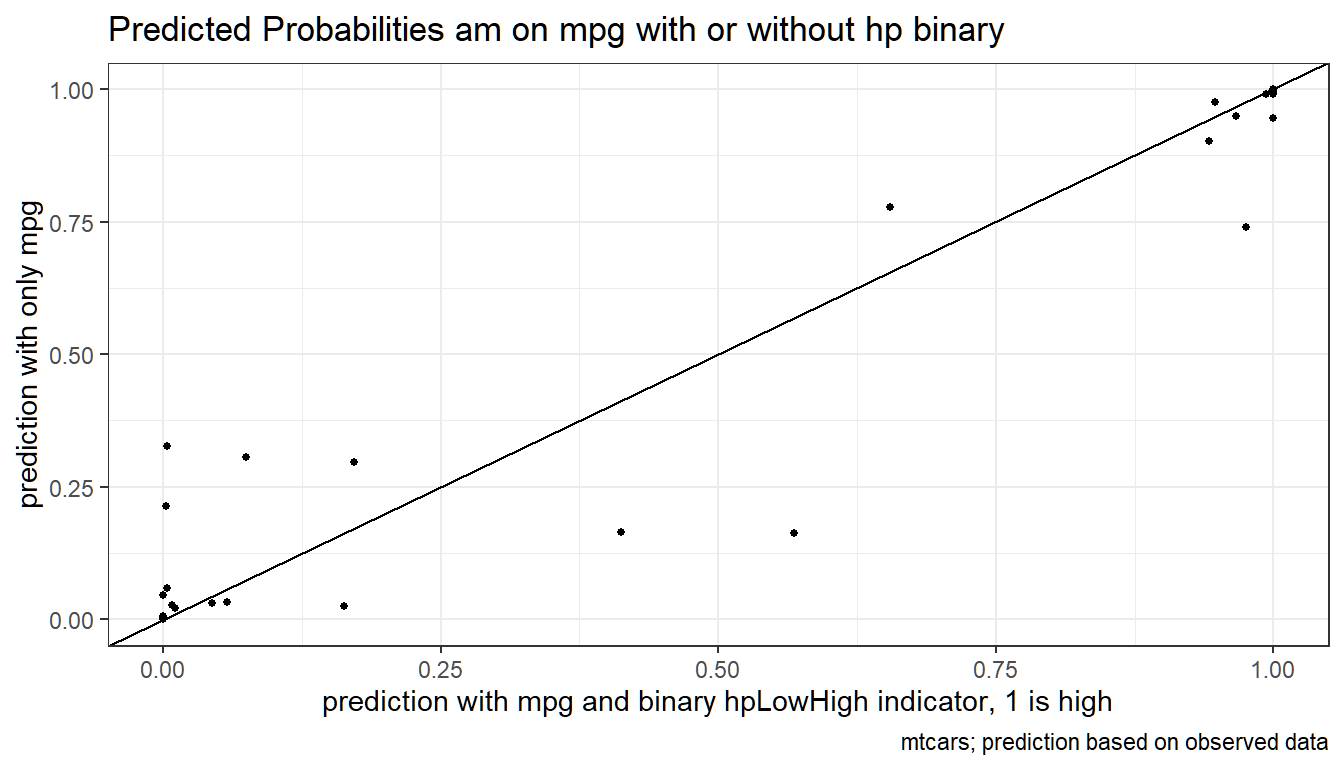
\includegraphics{Panel-Data-and-Optimization-with-R_files/figure-latex/logit with binary and continuous RHS-1} \end{center}

\hypertarget{prediction-with-binary-set-to-0-and-1}{%
\paragraph{Prediction with Binary set to 0 and 1}\label{prediction-with-binary-set-to-0-and-1}}

Now generate two predictions. One set where binary input is equal to 0, and another where the binary inputs are equal to 1. Ignore whether in data binary input is equal to 0 or 1. Use the same regression results as what was just derived.

Note that given the example here, the probability changes a lot when we

\begin{Shaded}
\begin{Highlighting}[]
\CommentTok{# Previous regression results}
\KeywordTok{summary}\NormalTok{(rs_logit_bi)}
\end{Highlighting}
\end{Shaded}

\begin{verbatim}
## 
## Call:
## glm(formula = as.formula(paste(svr_outcome, "~ factor(", svr_binary, 
##     ") + ", paste(ls_st_xs, collapse = "+"))), family = "binomial", 
##     data = df_mtcars)
## 
## Deviance Residuals: 
##      Min        1Q    Median        3Q       Max  
## -1.45771  -0.09563  -0.00875   0.00555   1.87612  
## 
## Coefficients:
##                         Estimate Std. Error z value Pr(>|z|)  
## (Intercept)               3.8285    18.0390   0.212   0.8319  
## factor(hpLowHigh)HighHP   6.9907     5.5176   1.267   0.2052  
## mpg                       0.8985     0.8906   1.009   0.3131  
## wt                       -6.7291     3.3166  -2.029   0.0425 *
## vs                       -5.9206     4.1908  -1.413   0.1577  
## ---
## Signif. codes:  0 '***' 0.001 '**' 0.01 '*' 0.05 '.' 0.1 ' ' 1
## 
## (Dispersion parameter for binomial family taken to be 1)
## 
##     Null deviance: 43.2297  on 31  degrees of freedom
## Residual deviance:  8.9777  on 27  degrees of freedom
## AIC: 18.978
## 
## Number of Fisher Scoring iterations: 9
\end{verbatim}

\begin{Shaded}
\begin{Highlighting}[]
\CommentTok{# Two different dataframes, mutate the binary regressor}
\NormalTok{df_mtcars_bi0 <-}\StringTok{ }\NormalTok{df_mtcars }\OperatorTok\StringTok{ }\KeywordTok{mutate}\NormalTok{(}\OperatorTok{!!}\KeywordTok{sym}\NormalTok{(svr_binary) }\OperatorTok{:}\ErrorTok{=}\StringTok{ }\NormalTok{svr_binary_lb0)}
\NormalTok{df_mtcars_bi1 <-}\StringTok{ }\NormalTok{df_mtcars }\OperatorTok\StringTok{ }\KeywordTok{mutate}\NormalTok{(}\OperatorTok{!!}\KeywordTok{sym}\NormalTok{(svr_binary) }\OperatorTok{:}\ErrorTok{=}\StringTok{ }\NormalTok{svr_binary_lb1)}

\CommentTok{# Predcit Using Regresion Data}
\NormalTok{df_mtcars}\OperatorTok{$}\NormalTok{p_mpg_hp_bi0 <-}\StringTok{ }\KeywordTok{predict}\NormalTok{(rs_logit_bi, }\DataTypeTok{newdata =}\NormalTok{ df_mtcars_bi0, }\DataTypeTok{type =} \StringTok{"response"}\NormalTok{)}
\NormalTok{df_mtcars}\OperatorTok{$}\NormalTok{p_mpg_hp_bi1 <-}\StringTok{ }\KeywordTok{predict}\NormalTok{(rs_logit_bi, }\DataTypeTok{newdata =}\NormalTok{ df_mtcars_bi1, }\DataTypeTok{type =} \StringTok{"response"}\NormalTok{)}

\CommentTok{# Predicted Probabilities and Binary Input}
\NormalTok{scatter <-}\StringTok{ }\KeywordTok{ggplot}\NormalTok{(df_mtcars, }\KeywordTok{aes}\NormalTok{(}\DataTypeTok{x=}\NormalTok{p_mpg_hp_bi0)) }\OperatorTok{+}
\StringTok{      }\KeywordTok{geom_point}\NormalTok{(}\KeywordTok{aes}\NormalTok{(}\DataTypeTok{y=}\NormalTok{p_mpg_hp), }\DataTypeTok{size=}\DecValTok{4}\NormalTok{, }\DataTypeTok{shape=}\DecValTok{4}\NormalTok{, }\DataTypeTok{color=}\StringTok{"red"}\NormalTok{) }\OperatorTok{+}
\StringTok{      }\KeywordTok{geom_point}\NormalTok{(}\KeywordTok{aes}\NormalTok{(}\DataTypeTok{y=}\NormalTok{p_mpg_hp_bi1), }\DataTypeTok{size=}\DecValTok{2}\NormalTok{, }\DataTypeTok{shape=}\DecValTok{8}\NormalTok{) }\OperatorTok{+}
\StringTok{      }\CommentTok{# geom_smooth(method=lm) + # Trend line}
\StringTok{      }\KeywordTok{geom_abline}\NormalTok{(}\DataTypeTok{intercept =} \DecValTok{0}\NormalTok{, }\DataTypeTok{slope =} \DecValTok{1}\NormalTok{) }\OperatorTok{+}\StringTok{ }\CommentTok{# 45 degree line}
\StringTok{      }\KeywordTok{labs}\NormalTok{(}\DataTypeTok{title =} \KeywordTok{paste0}\NormalTok{(}\StringTok{'Predicted Probabilities and Binary Input'}\NormalTok{,}
                          \StringTok{'}\CharTok{\textbackslash{}n}\StringTok{cross(shape=4)/red is predict actual binary data'}\NormalTok{,}
                          \StringTok{'}\CharTok{\textbackslash{}n}\StringTok{star(shape=8)/black is predict set binary = 1 for all'}\NormalTok{),}
            \DataTypeTok{x =} \KeywordTok{paste0}\NormalTok{(}\StringTok{'prediction with '}\NormalTok{, ls_st_xs, }\StringTok{' and binary '}\NormalTok{, svr_binary, }\StringTok{' = 0 for all'}\NormalTok{),}
            \DataTypeTok{y =} \KeywordTok{paste0}\NormalTok{(}\StringTok{'prediction with '}\NormalTok{, ls_st_xs, }\StringTok{' and binary '}\NormalTok{, svr_binary, }\StringTok{' = 1'}\NormalTok{),}
           \DataTypeTok{caption =} \KeywordTok{paste0}\NormalTok{(sdt_name)) }\OperatorTok{+}
\StringTok{      }\KeywordTok{theme_bw}\NormalTok{()}
\KeywordTok{print}\NormalTok{(scatter)}
\end{Highlighting}
\end{Shaded}

\begin{center}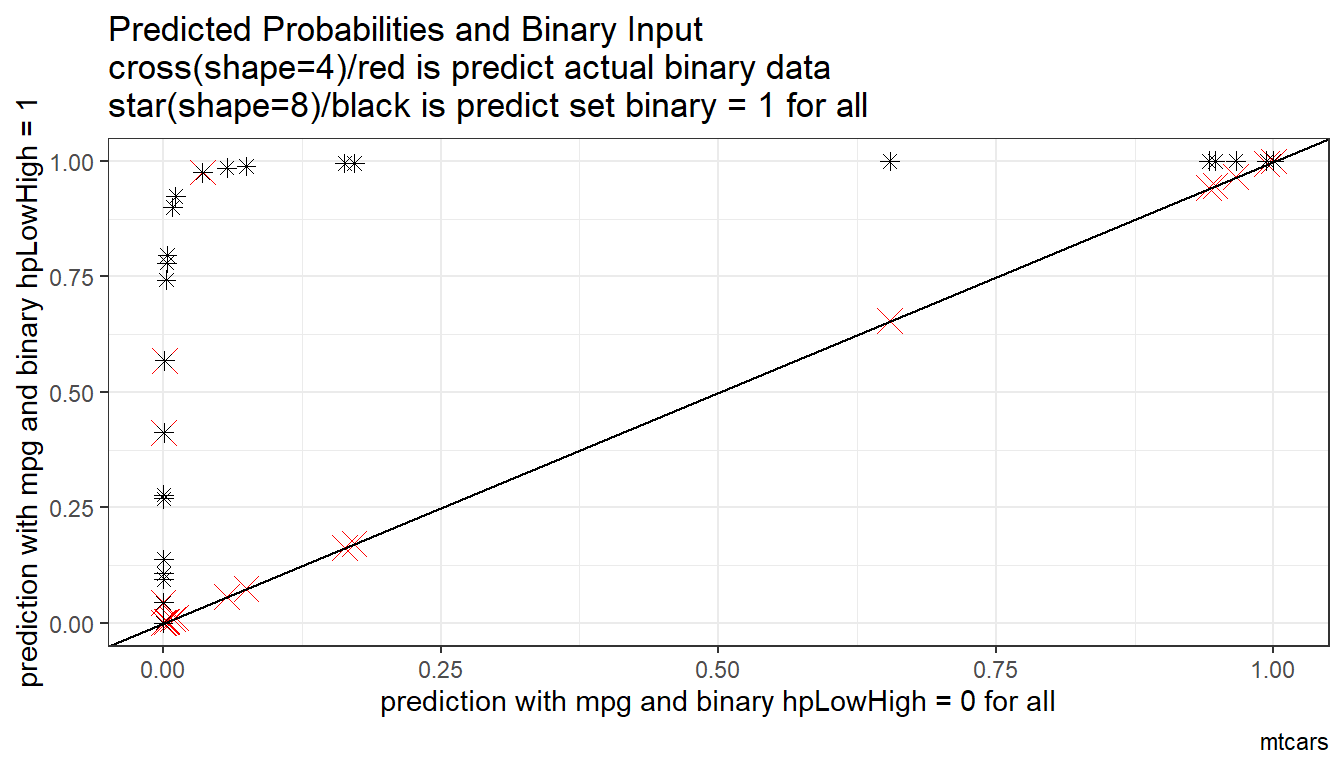
\includegraphics{Panel-Data-and-Optimization-with-R_files/figure-latex/logit prediction 0 vs 1-1} \end{center}

\hypertarget{prediction-with-binary-set-to-0-and-1-difference}{%
\paragraph{Prediction with Binary set to 0 and 1 Difference}\label{prediction-with-binary-set-to-0-and-1-difference}}

What is the difference in probability between binary = 0 vs binary = 1. How does that relate to the probability of outcome of interest when binary = 0 for all.

In the binary logit case, the relationship will be hump--shaped by construction between \(A_i\) and \(\alpha_i\). In the exponential wage cases, the relationship is convex upwards.

\begin{Shaded}
\begin{Highlighting}[]
\CommentTok{# Generate Gap Variable}
\NormalTok{df_mtcars <-}\StringTok{ }\NormalTok{df_mtcars }\OperatorTok\StringTok{ }\KeywordTok{mutate}\NormalTok{(}\DataTypeTok{alpha_i =}\NormalTok{ p_mpg_hp_bi1 }\OperatorTok{-}\StringTok{ }\NormalTok{p_mpg_hp_bi0) }\OperatorTok
\StringTok{                }\KeywordTok{mutate}\NormalTok{(}\DataTypeTok{A_i =}\NormalTok{ p_mpg_hp_bi0)}

\CommentTok{# Binary Marginal Effects and Prediction without Binary}
\NormalTok{scatter <-}\StringTok{ }\KeywordTok{ggplot}\NormalTok{(df_mtcars, }\KeywordTok{aes}\NormalTok{(}\DataTypeTok{x=}\NormalTok{A_i)) }\OperatorTok{+}
\StringTok{      }\KeywordTok{geom_point}\NormalTok{(}\KeywordTok{aes}\NormalTok{(}\DataTypeTok{y=}\NormalTok{alpha_i), }\DataTypeTok{size=}\DecValTok{4}\NormalTok{, }\DataTypeTok{shape=}\DecValTok{4}\NormalTok{, }\DataTypeTok{color=}\StringTok{"red"}\NormalTok{) }\OperatorTok{+}
\StringTok{      }\KeywordTok{geom_abline}\NormalTok{(}\DataTypeTok{intercept =} \DecValTok{0}\NormalTok{, }\DataTypeTok{slope =} \DecValTok{1}\NormalTok{) }\OperatorTok{+}\StringTok{ }\CommentTok{# 45 degree line}
\StringTok{      }\KeywordTok{labs}\NormalTok{(}\DataTypeTok{title =} \KeywordTok{paste0}\NormalTok{(}\StringTok{'Binary Marginal Effects and Prediction without Binary'}\NormalTok{),}
           \DataTypeTok{x =} \StringTok{'P(binary=0) for all'}\NormalTok{,}
           \DataTypeTok{y =} \StringTok{'P(binary=1) - P(binary=0) gap'}\NormalTok{,}
           \DataTypeTok{caption =} \KeywordTok{paste0}\NormalTok{(sdt_name)) }\OperatorTok{+}
\StringTok{      }\KeywordTok{theme_bw}\NormalTok{()}
\KeywordTok{print}\NormalTok{(scatter)}
\end{Highlighting}
\end{Shaded}

\begin{center}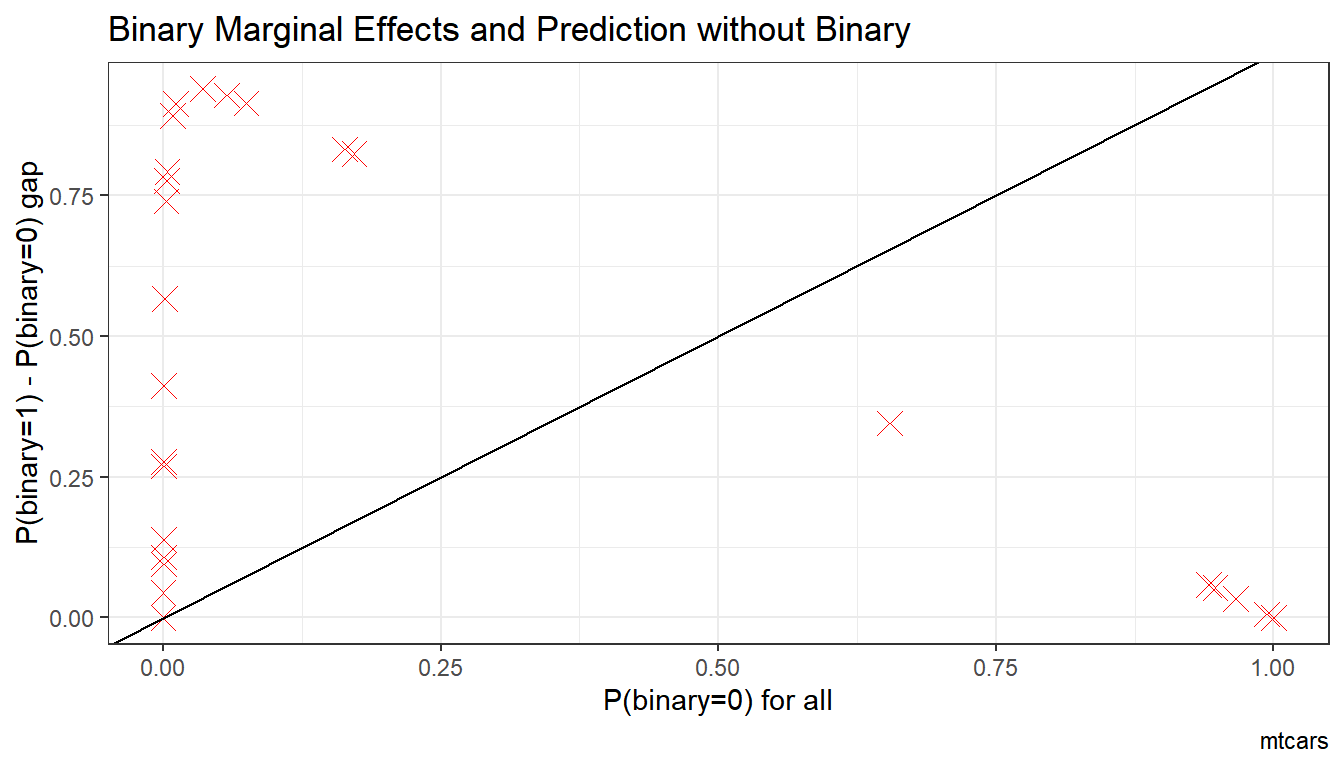
\includegraphics{Panel-Data-and-Optimization-with-R_files/figure-latex/logit prediction marginal vs base-1} \end{center}

\hypertarget{x-variables-and-a-and-alpha}{%
\paragraph{X variables and A and alpha}\label{x-variables-and-a-and-alpha}}

Given the x-variables included in the logit regression, how do they relate to A\_i and alpha\_i

\begin{Shaded}
\begin{Highlighting}[]
\CommentTok{# Generate Gap Variable}
\NormalTok{df_mtcars <-}\StringTok{ }\NormalTok{df_mtcars }\OperatorTok\StringTok{ }\KeywordTok{mutate}\NormalTok{(}\DataTypeTok{alpha_i =}\NormalTok{ p_mpg_hp_bi1 }\OperatorTok{-}\StringTok{ }\NormalTok{p_mpg_hp_bi0) }\OperatorTok
\StringTok{                }\KeywordTok{mutate}\NormalTok{(}\DataTypeTok{A_i =}\NormalTok{ p_mpg_hp_bi0)}

\CommentTok{# Binary Marginal Effects and Prediction without Binary}
\NormalTok{ggplot.A.alpha.x <-}\StringTok{ }\ControlFlowTok{function}\NormalTok{(svr_x, df,}
                             \DataTypeTok{svr_alpha =} \StringTok{'alpha_i'}\NormalTok{, }\DataTypeTok{svr_A =} \StringTok{"A_i"}\NormalTok{)\{}

\NormalTok{  scatter <-}\StringTok{ }\KeywordTok{ggplot}\NormalTok{(df, }\KeywordTok{aes}\NormalTok{(}\DataTypeTok{x=}\OperatorTok{!!}\KeywordTok{sym}\NormalTok{(svr_x))) }\OperatorTok{+}
\StringTok{        }\KeywordTok{geom_point}\NormalTok{(}\KeywordTok{aes}\NormalTok{(}\DataTypeTok{y=}\NormalTok{alpha_i), }\DataTypeTok{size=}\DecValTok{4}\NormalTok{, }\DataTypeTok{shape=}\DecValTok{4}\NormalTok{, }\DataTypeTok{color=}\StringTok{"red"}\NormalTok{) }\OperatorTok{+}
\StringTok{        }\KeywordTok{geom_point}\NormalTok{(}\KeywordTok{aes}\NormalTok{(}\DataTypeTok{y=}\NormalTok{A_i), }\DataTypeTok{size=}\DecValTok{2}\NormalTok{, }\DataTypeTok{shape=}\DecValTok{8}\NormalTok{, }\DataTypeTok{color=}\StringTok{"blue"}\NormalTok{) }\OperatorTok{+}
\StringTok{        }\KeywordTok{geom_abline}\NormalTok{(}\DataTypeTok{intercept =} \DecValTok{0}\NormalTok{, }\DataTypeTok{slope =} \DecValTok{1}\NormalTok{) }\OperatorTok{+}\StringTok{ }\CommentTok{# 45 degree line}
\StringTok{        }\KeywordTok{labs}\NormalTok{(}\DataTypeTok{title =} \KeywordTok{paste0}\NormalTok{(}\StringTok{'A (blue) and alpha (red) vs x variables='}\NormalTok{, svr_x),}
             \DataTypeTok{x =}\NormalTok{ svr_x,}
             \DataTypeTok{y =} \StringTok{'Probabilities'}\NormalTok{,}
             \DataTypeTok{caption =} \KeywordTok{paste0}\NormalTok{(sdt_name)) }\OperatorTok{+}
\StringTok{        }\KeywordTok{theme_bw}\NormalTok{()}

\KeywordTok{return}\NormalTok{(scatter)}
\NormalTok{\}}

\CommentTok{# Plot over multiple}
\KeywordTok{lapply}\NormalTok{(ls_st_xs,}
\NormalTok{       ggplot.A.alpha.x,}
       \DataTypeTok{df =}\NormalTok{ df_mtcars)}
\end{Highlighting}
\end{Shaded}

\begin{verbatim}
## [[1]]
\end{verbatim}

\begin{center}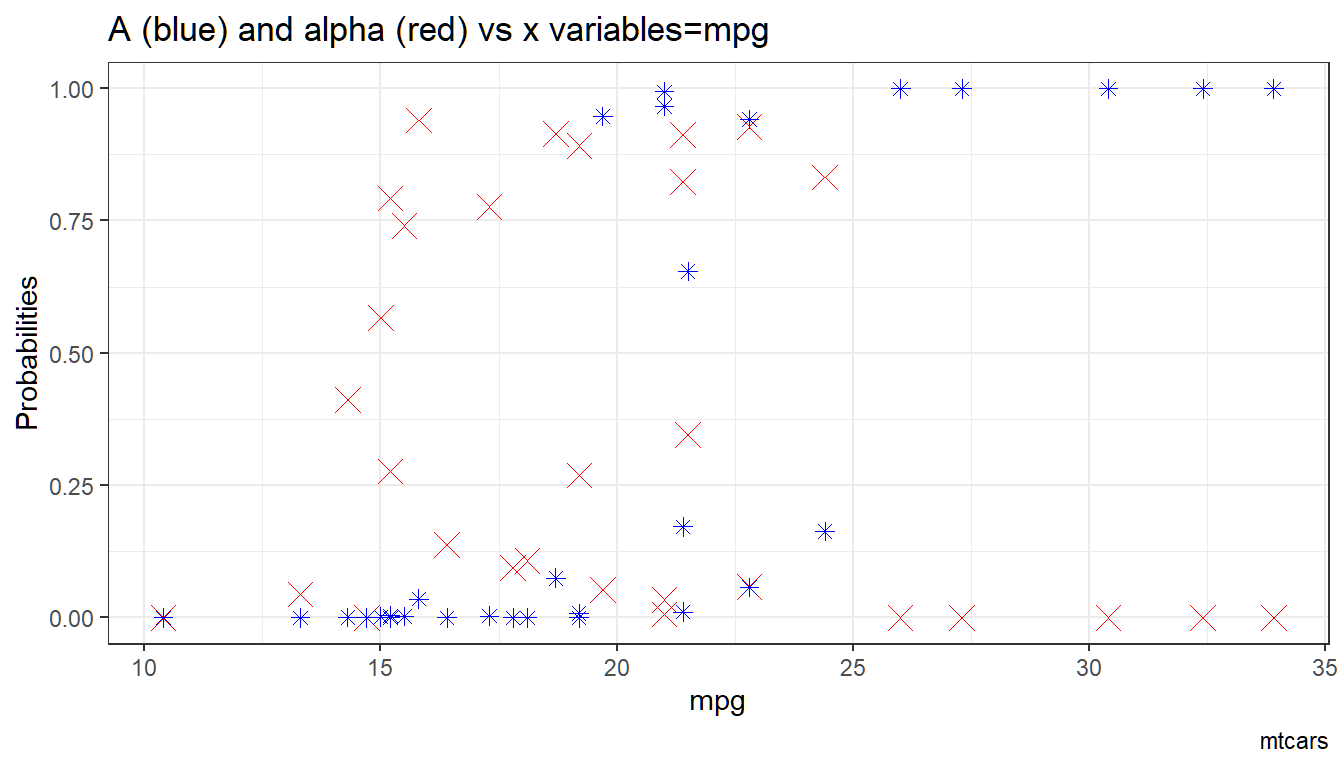
\includegraphics{Panel-Data-and-Optimization-with-R_files/figure-latex/unnamed-chunk-149-1} \end{center}

\begin{verbatim}
## 
## [[2]]
\end{verbatim}

\begin{center}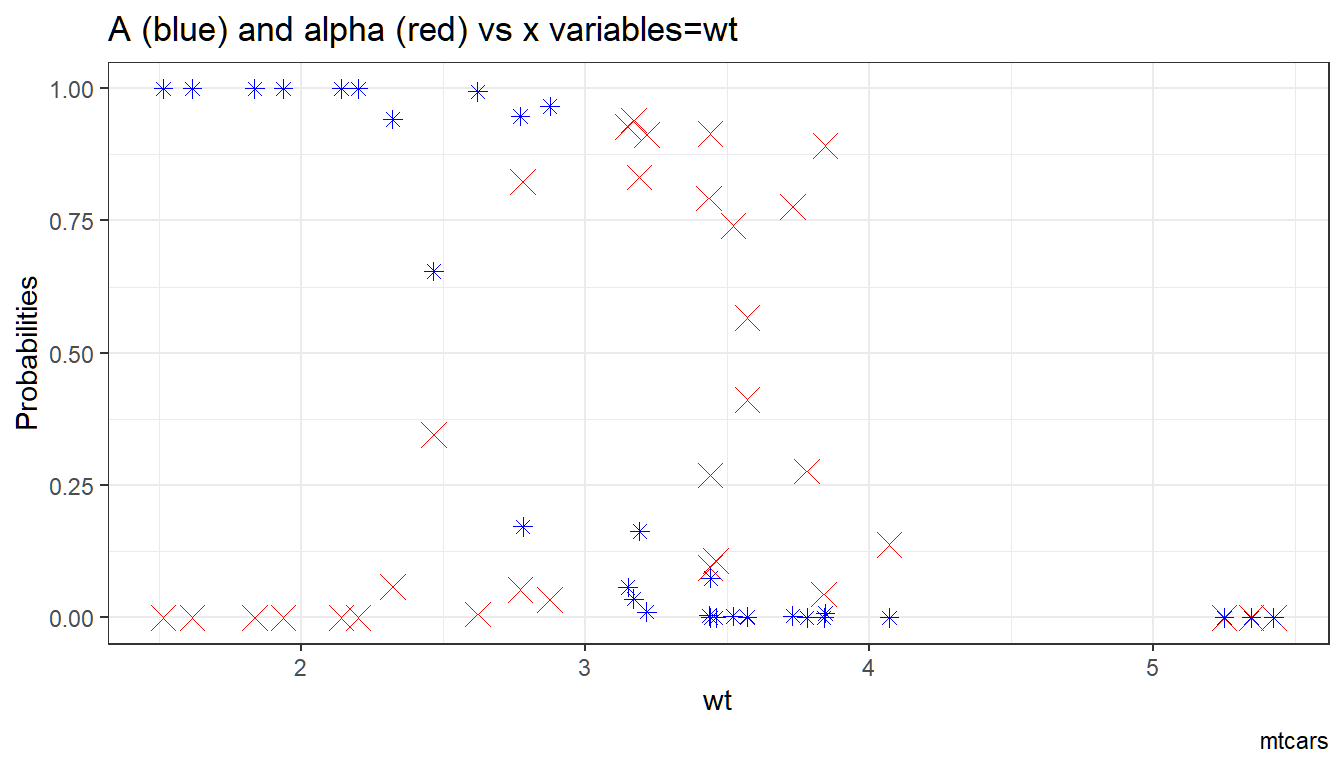
\includegraphics{Panel-Data-and-Optimization-with-R_files/figure-latex/unnamed-chunk-149-2} \end{center}

\begin{verbatim}
## 
## [[3]]
\end{verbatim}

\begin{center}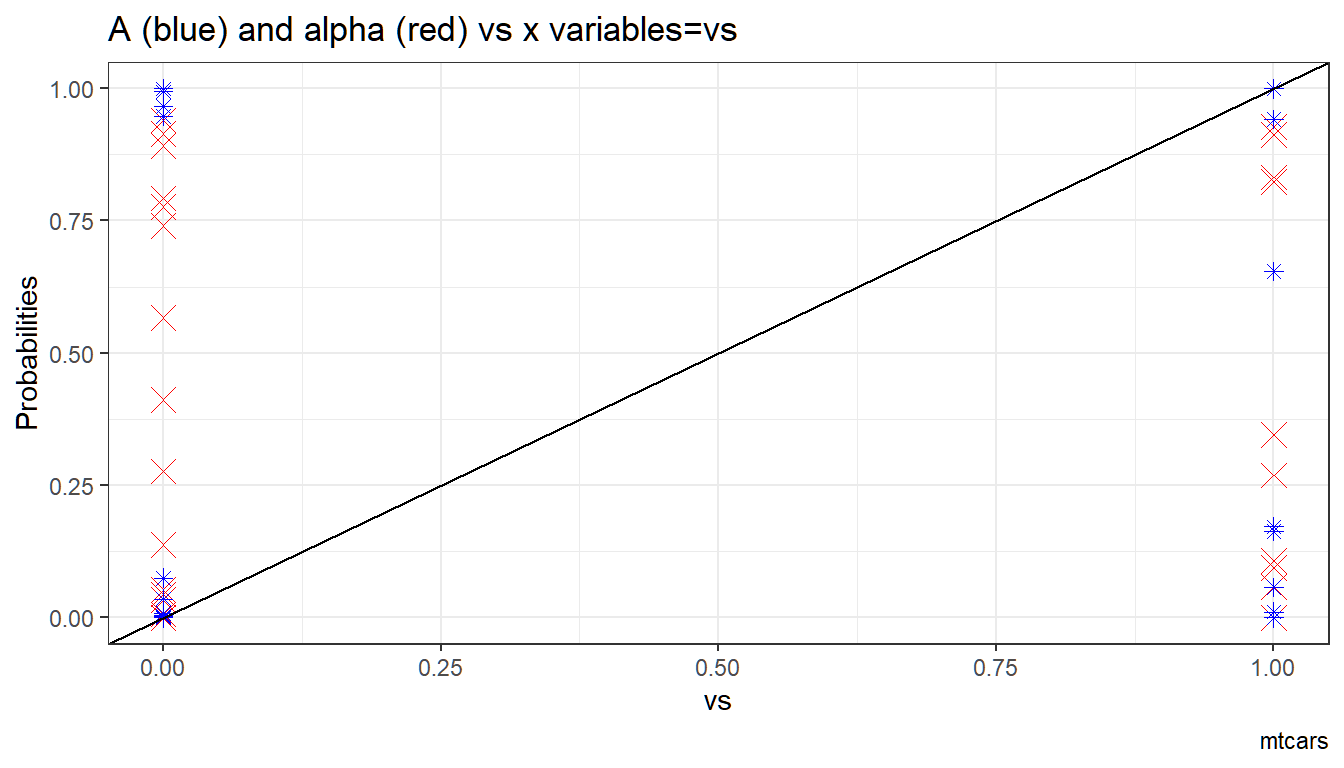
\includegraphics{Panel-Data-and-Optimization-with-R_files/figure-latex/unnamed-chunk-149-3} \end{center}

\hypertarget{optimization}{%
\chapter{Optimization}\label{optimization}}

\hypertarget{bisection}{%
\section{Bisection}\label{bisection}}

\hypertarget{bisection-1}{%
\subsection{Bisection}\label{bisection-1}}

\begin{quote}
Go back to \href{http://fanwangecon.github.io/}{fan}'s \href{https://fanwangecon.github.io/REconTools/}{REconTools} Package, \href{https://fanwangecon.github.io/R4Econ/}{R4Econ} Repository (\href{https://fanwangecon.github.io/R4Econ/bookdown}{bookdown site}), or \href{https://fanwangecon.github.io/Stat4Econ/}{Intro Stats with R} Repository.
\end{quote}

See the \href{https://fanwangecon.github.io/REconTools/reference/ff_opti_bisect_pmap_multi.html}{ff\_opti\_bisect\_pmap\_multi} function from \href{https://fanwangecon.github.io/}{Fan}'s \emph{\href{https://fanwangecon.github.io/REconTools/}{REconTools}} Package, which provides a resuable function based on the algorithm worked out here.

The bisection specific code does not need to do much.

\begin{itemize}
\tightlist
\item
  list variables in file for grouping, each group is an individual for whom we want to calculate optimal choice for using bisection.
\item
  string variable name of input where functions are evaluated, these are already contained in the dataframe, existing variable names, row specific, rowwise computation over these, each rowwise calculation using different rows.
\item
  scalar and array values that are applied to every rowwise calculation, all rowwise calculations using the same scalars and arrays.
\item
  string output variable name
\end{itemize}

This is how I implement the bisection algorithm, when we know the bounding minimum and maximum to be below and above zero already.

\begin{enumerate}
\def\labelenumi{\arabic{enumi}.}
\tightlist
\item
  Evaluate \(f^0_a = f(a^0)\) and \(f^0_b = f(b^0)\), min and max points.
\item
  Evaluate at \(f^0_p = f(p^0)\), where \(p_0 = \frac{a^0+b^0}{2}\).
\item
  if \(f^i_a \cdot f^i_p < 0\), then \(b_{i+1} = p_i\), else, \(a_{i+1} = p_i\) and \(f^{i+1}_a = p_i\).
\item
  iteratre until convergence.
\end{enumerate}

Generate New columns of a and b as we iteratre, do not need to store p, p is temporary. Evaluate the function below which we have already tested, but now, in the dataframe before generating all permutations, \emph{tb\_states\_choices}, now the \emph{fl\_N} element will be changing with each iteration, it will be row specific. \emph{fl\_N} are first min and max, then each subsequent ps.

\hypertarget{initialize-matrix}{%
\subsubsection{Initialize Matrix}\label{initialize-matrix}}

First, initialize the matrix with \(a_0\) and \(b_0\), the initial min and max points:

\begin{Shaded}
\begin{Highlighting}[]
\CommentTok{# common prefix to make reshaping easier}
\NormalTok{st_bisec_prefix <-}\StringTok{ 'bisec_'}
\NormalTok{svr_a_lst <-}\StringTok{ }\KeywordTok{paste0}\NormalTok{(st_bisec_prefix, }\StringTok{'a_0'}\NormalTok{)}
\NormalTok{svr_b_lst <-}\StringTok{ }\KeywordTok{paste0}\NormalTok{(st_bisec_prefix, }\StringTok{'b_0'}\NormalTok{)}
\NormalTok{svr_fa_lst <-}\StringTok{ }\KeywordTok{paste0}\NormalTok{(st_bisec_prefix, }\StringTok{'fa_0'}\NormalTok{)}
\NormalTok{svr_fb_lst <-}\StringTok{ }\KeywordTok{paste0}\NormalTok{(st_bisec_prefix, }\StringTok{'fb_0'}\NormalTok{)}

\CommentTok{# Add initial a and b}
\NormalTok{tb_states_choices_bisec <-}\StringTok{ }\NormalTok{tb_states_choices }\OperatorTok
\StringTok{  }\KeywordTok{mutate}\NormalTok{(}\OperatorTok{!!}\KeywordTok{sym}\NormalTok{(svr_a_lst) }\OperatorTok{:}\ErrorTok{=}\StringTok{ }\NormalTok{fl_N_min, }\OperatorTok{!!}\KeywordTok{sym}\NormalTok{(svr_b_lst) }\OperatorTok{:}\ErrorTok{=}\StringTok{ }\NormalTok{fl_N_agg)}

\CommentTok{# Evaluate function f(a_0) and f(b_0)}
\NormalTok{tb_states_choices_bisec <-}\StringTok{ }\NormalTok{tb_states_choices_bisec }\OperatorTok
\StringTok{  }\KeywordTok{rowwise}\NormalTok{() }\OperatorTok
\StringTok{  }\KeywordTok{mutate}\NormalTok{(}\OperatorTok{!!}\KeywordTok{sym}\NormalTok{(svr_fa_lst) }\OperatorTok{:}\ErrorTok{=}\StringTok{ }\KeywordTok{ffi_nonlin_dplyrdo}\NormalTok{(fl_A, fl_alpha, }\OperatorTok{!!}\KeywordTok{sym}\NormalTok{(svr_a_lst),}
\NormalTok{                                                ar_nN_A, ar_nN_alpha,}
\NormalTok{                                                fl_N_agg, fl_rho),}
         \OperatorTok{!!}\KeywordTok{sym}\NormalTok{(svr_fb_lst) }\OperatorTok{:}\ErrorTok{=}\StringTok{ }\KeywordTok{ffi_nonlin_dplyrdo}\NormalTok{(fl_A, fl_alpha, }\OperatorTok{!!}\KeywordTok{sym}\NormalTok{(svr_b_lst),}
\NormalTok{                                                ar_nN_A, ar_nN_alpha,}
\NormalTok{                                                fl_N_agg, fl_rho))}
\CommentTok{# Summarize}
\KeywordTok{dim}\NormalTok{(tb_states_choices_bisec)}
\end{Highlighting}
\end{Shaded}

\begin{verbatim}
## [1] 4 7
\end{verbatim}

\begin{Shaded}
\begin{Highlighting}[]
\CommentTok{# summary(tb_states_choices_bisec)}
\end{Highlighting}
\end{Shaded}

\hypertarget{iterate-and-solve-for-fp-update-fa-and-fb}{%
\subsubsection{Iterate and Solve for f(p), update f(a) and f(b)}\label{iterate-and-solve-for-fp-update-fa-and-fb}}

Implement the DPLYR based Concurrent bisection algorithm.

\begin{Shaded}
\begin{Highlighting}[]
\CommentTok{# fl_tol = float tolerance criteria}
\CommentTok{# it_tol = number of interations to allow at most}
\NormalTok{fl_tol <-}\StringTok{ }\DecValTok{10}\OperatorTok{^-}\DecValTok{2}
\NormalTok{it_tol <-}\StringTok{ }\DecValTok{100}

\CommentTok{# fl_p_dist2zr = distance to zero to initalize}
\NormalTok{fl_p_dist2zr <-}\StringTok{ }\DecValTok{1000}
\NormalTok{it_cur <-}\StringTok{ }\DecValTok{0}
\ControlFlowTok{while}\NormalTok{ (it_cur }\OperatorTok{<=}\StringTok{ }\NormalTok{it_tol }\OperatorTok{&&}\StringTok{ }\NormalTok{fl_p_dist2zr }\OperatorTok{>=}\StringTok{ }\NormalTok{fl_tol ) \{}

\NormalTok{  it_cur <-}\StringTok{ }\NormalTok{it_cur }\OperatorTok{+}\StringTok{ }\DecValTok{1}

  \CommentTok{# New Variables}
\NormalTok{  svr_a_cur <-}\StringTok{ }\KeywordTok{paste0}\NormalTok{(st_bisec_prefix, }\StringTok{'a_'}\NormalTok{, it_cur)}
\NormalTok{  svr_b_cur <-}\StringTok{ }\KeywordTok{paste0}\NormalTok{(st_bisec_prefix, }\StringTok{'b_'}\NormalTok{, it_cur)}
\NormalTok{  svr_fa_cur <-}\StringTok{ }\KeywordTok{paste0}\NormalTok{(st_bisec_prefix, }\StringTok{'fa_'}\NormalTok{, it_cur)}
\NormalTok{  svr_fb_cur <-}\StringTok{ }\KeywordTok{paste0}\NormalTok{(st_bisec_prefix, }\StringTok{'fb_'}\NormalTok{, it_cur)}

  \CommentTok{# Evaluate function f(a_0) and f(b_0)}
  \CommentTok{# 1. generate p}
  \CommentTok{# 2. generate f_p}
  \CommentTok{# 3. generate f_p*f_a}
\NormalTok{  tb_states_choices_bisec <-}\StringTok{ }\NormalTok{tb_states_choices_bisec }\OperatorTok
\StringTok{    }\KeywordTok{rowwise}\NormalTok{() }\OperatorTok
\StringTok{    }\KeywordTok{mutate}\NormalTok{(}\DataTypeTok{p =}\NormalTok{ ((}\OperatorTok{!!}\KeywordTok{sym}\NormalTok{(svr_a_lst) }\OperatorTok{+}\StringTok{ }\OperatorTok{!!}\KeywordTok{sym}\NormalTok{(svr_b_lst))}\OperatorTok{/}\DecValTok{2}\NormalTok{)) }\OperatorTok
\StringTok{    }\KeywordTok{mutate}\NormalTok{(}\DataTypeTok{f_p =} \KeywordTok{ffi_nonlin_dplyrdo}\NormalTok{(fl_A, fl_alpha, p,}
\NormalTok{                                    ar_nN_A, ar_nN_alpha,}
\NormalTok{                                    fl_N_agg, fl_rho)) }\OperatorTok
\StringTok{    }\KeywordTok{mutate}\NormalTok{(}\DataTypeTok{f_p_t_f_a =}\NormalTok{ f_p}\OperatorTok{*!!}\KeywordTok{sym}\NormalTok{(svr_fa_lst))}
  \CommentTok{# fl_p_dist2zr = sum(abs(p))}
\NormalTok{  fl_p_dist2zr <-}\StringTok{ }\KeywordTok{mean}\NormalTok{(}\KeywordTok{abs}\NormalTok{(tb_states_choices_bisec }\OperatorTok\StringTok{ }\KeywordTok{pull}\NormalTok{(f_p)))}

  \CommentTok{# Update a and b}
\NormalTok{  tb_states_choices_bisec <-}\StringTok{ }\NormalTok{tb_states_choices_bisec }\OperatorTok
\StringTok{    }\KeywordTok{mutate}\NormalTok{(}\OperatorTok{!!}\KeywordTok{sym}\NormalTok{(svr_a_cur) }\OperatorTok{:}\ErrorTok{=}
\StringTok{             }\KeywordTok{case_when}\NormalTok{(f_p_t_f_a }\OperatorTok{<}\StringTok{ }\DecValTok{0} \OperatorTok{~}\StringTok{ }\OperatorTok{!!}\KeywordTok{sym}\NormalTok{(svr_a_lst),}
                       \OtherTok{TRUE} \OperatorTok{~}\StringTok{ }\NormalTok{p)) }\OperatorTok
\StringTok{    }\KeywordTok{mutate}\NormalTok{(}\OperatorTok{!!}\KeywordTok{sym}\NormalTok{(svr_b_cur) }\OperatorTok{:}\ErrorTok{=}
\StringTok{             }\KeywordTok{case_when}\NormalTok{(f_p_t_f_a }\OperatorTok{<}\StringTok{ }\DecValTok{0} \OperatorTok{~}\StringTok{ }\NormalTok{p,}
                       \OtherTok{TRUE} \OperatorTok{~}\StringTok{ }\OperatorTok{!!}\KeywordTok{sym}\NormalTok{(svr_b_lst)))}
  \CommentTok{# Update f(a) and f(b)}
\NormalTok{  tb_states_choices_bisec <-}\StringTok{ }\NormalTok{tb_states_choices_bisec }\OperatorTok
\StringTok{    }\KeywordTok{mutate}\NormalTok{(}\OperatorTok{!!}\KeywordTok{sym}\NormalTok{(svr_fa_cur) }\OperatorTok{:}\ErrorTok{=}
\StringTok{             }\KeywordTok{case_when}\NormalTok{(f_p_t_f_a }\OperatorTok{<}\StringTok{ }\DecValTok{0} \OperatorTok{~}\StringTok{ }\OperatorTok{!!}\KeywordTok{sym}\NormalTok{(svr_fa_lst),}
                       \OtherTok{TRUE} \OperatorTok{~}\StringTok{ }\NormalTok{f_p)) }\OperatorTok
\StringTok{    }\KeywordTok{mutate}\NormalTok{(}\OperatorTok{!!}\KeywordTok{sym}\NormalTok{(svr_fb_cur) }\OperatorTok{:}\ErrorTok{=}
\StringTok{             }\KeywordTok{case_when}\NormalTok{(f_p_t_f_a }\OperatorTok{<}\StringTok{ }\DecValTok{0} \OperatorTok{~}\StringTok{ }\NormalTok{f_p,}
                       \OtherTok{TRUE} \OperatorTok{~}\StringTok{ }\OperatorTok{!!}\KeywordTok{sym}\NormalTok{(svr_fb_lst)))}
  \CommentTok{# Save from last}
\NormalTok{  svr_a_lst <-}\StringTok{ }\NormalTok{svr_a_cur}
\NormalTok{  svr_b_lst <-}\StringTok{ }\NormalTok{svr_b_cur}
\NormalTok{  svr_fa_lst <-}\StringTok{ }\NormalTok{svr_fa_cur}
\NormalTok{  svr_fb_lst <-}\StringTok{ }\NormalTok{svr_fb_cur}

  \CommentTok{# Summar current round}
  \KeywordTok{print}\NormalTok{(}\KeywordTok{paste0}\NormalTok{(}\StringTok{'it_cur:'}\NormalTok{, it_cur, }\StringTok{', fl_p_dist2zr:'}\NormalTok{, fl_p_dist2zr))}
  \KeywordTok{summary}\NormalTok{(tb_states_choices_bisec }\OperatorTok
\StringTok{            }\KeywordTok{select}\NormalTok{(}\KeywordTok{one_of}\NormalTok{(svr_a_cur, svr_b_cur, svr_fa_cur, svr_fb_cur)))}
\NormalTok{\}}
\end{Highlighting}
\end{Shaded}

\begin{verbatim}
## [1] "it_cur:1, fl_p_dist2zr:1884.20860322127"
## [1] "it_cur:2, fl_p_dist2zr:815.07213515036"
## [1] "it_cur:3, fl_p_dist2zr:346.193951089409"
## [1] "it_cur:4, fl_p_dist2zr:133.268318242343"
## [1] "it_cur:5, fl_p_dist2zr:52.0759336601643"
## [1] "it_cur:6, fl_p_dist2zr:8.2057326579422"
## [1] "it_cur:7, fl_p_dist2zr:12.7240911320081"
## [1] "it_cur:8, fl_p_dist2zr:4.10100732130902"
## [1] "it_cur:9, fl_p_dist2zr:1.19915237247596"
## [1] "it_cur:10, fl_p_dist2zr:1.46089191924225"
## [1] "it_cur:11, fl_p_dist2zr:0.261965457555881"
## [1] "it_cur:12, fl_p_dist2zr:0.462901483859291"
## [1] "it_cur:13, fl_p_dist2zr:0.166336071560483"
## [1] "it_cur:14, fl_p_dist2zr:0.011649263648799"
## [1] "it_cur:15, fl_p_dist2zr:0.0715183716517558"
## [1] "it_cur:16, fl_p_dist2zr:0.0299376539319738"
## [1] "it_cur:17, fl_p_dist2zr:0.0132655999120672"
## [1] "it_cur:18, fl_p_dist2zr:0.00317751042553027"
\end{verbatim}

\hypertarget{reshape-wide-to-long-to-wide}{%
\subsubsection{Reshape Wide to long to Wide}\label{reshape-wide-to-long-to-wide}}

To view results easily, how iterations improved to help us find the roots, convert table from wide to long. Pivot twice. This allows us to easily graph out how bisection is working out iterationby iteration.

Here, we will first show what the raw table looks like, the wide only table, and then show the long version, and finally the version that is medium wide.

\hypertarget{table-onevery-wide}{%
\paragraph{Table One--Very Wide}\label{table-onevery-wide}}

Show what the \emph{tb\_states\_choices\_bisec} looks like.

Variables are formatted like: \emph{bisec\_xx\_yy}, where yy is the iteration indicator, and xx is either a, b, fa, or fb.

\begin{Shaded}
\begin{Highlighting}[]
\CommentTok{# head(tb_states_choices_bisec, 10)}
\CommentTok{# str(tb_states_choices_bisec)}
\end{Highlighting}
\end{Shaded}

\hypertarget{table-twovery-wide-to-very-long}{%
\paragraph{Table Two--Very Wide to Very Long}\label{table-twovery-wide-to-very-long}}

We want to treat the iteration count information that is the suffix of variable names as a variable by itself. Additionally, we want to treat the a,b,fa,fb as a variable. Structuring the data very long like this allows for easy graphing and other types of analysis. Rather than dealing with many many variables, we have only 3 core variables that store bisection iteration information.

Here we use the very nice \emph{pivot\_longer} function. Note that to achieve this, we put a common prefix in front of the variables we wanted to convert to long. THis is helpful, because we can easily identify which variables need to be reshaped.

\begin{Shaded}
\begin{Highlighting}[]
\CommentTok{# New variables}
\NormalTok{svr_bisect_iter <-}\StringTok{ 'biseciter'}
\NormalTok{svr_abfafb_long_name <-}\StringTok{ 'varname'}
\NormalTok{svr_number_col <-}\StringTok{ 'value'}
\NormalTok{svr_id_bisect_iter <-}\StringTok{ }\KeywordTok{paste0}\NormalTok{(svr_id_var, }\StringTok{'_bisect_ier'}\NormalTok{)}

\CommentTok{# Pivot wide to very long}
\NormalTok{tb_states_choices_bisec_long <-}\StringTok{ }\NormalTok{tb_states_choices_bisec }\OperatorTok
\StringTok{  }\KeywordTok{pivot_longer}\NormalTok{(}
    \DataTypeTok{cols =} \KeywordTok{starts_with}\NormalTok{(st_bisec_prefix),}
    \DataTypeTok{names_to =} \KeywordTok{c}\NormalTok{(svr_abfafb_long_name, svr_bisect_iter),}
    \DataTypeTok{names_pattern =} \KeywordTok{paste0}\NormalTok{(st_bisec_prefix, }\StringTok{"(.*)_(.*)"}\NormalTok{),}
    \DataTypeTok{values_to =}\NormalTok{ svr_number_col}
\NormalTok{  )}

\CommentTok{# Print}
\CommentTok{# summary(tb_states_choices_bisec_long)}
\KeywordTok{head}\NormalTok{(tb_states_choices_bisec_long }\OperatorTok\StringTok{ }\KeywordTok{select}\NormalTok{(}\OperatorTok{-}\KeywordTok{one_of}\NormalTok{(}\StringTok{'p'}\NormalTok{,}\StringTok{'f_p'}\NormalTok{,}\StringTok{'f_p_t_f_a'}\NormalTok{)), }\DecValTok{30}\NormalTok{)}
\end{Highlighting}
\end{Shaded}

\begin{verbatim}
## # A tibble: 30 x 6
##    INDI_ID  fl_A fl_alpha varname biseciter   value
##      <int> <dbl>    <dbl> <chr>   <chr>       <dbl>
##  1       1    -2      0.1 a       0              0 
##  2       1    -2      0.1 b       0            100 
##  3       1    -2      0.1 fa      0            100 
##  4       1    -2      0.1 fb      0         -15058.
##  5       1    -2      0.1 a       1              0 
##  6       1    -2      0.1 b       1             50 
##  7       1    -2      0.1 fa      1            100 
##  8       1    -2      0.1 fb      1          -6660.
##  9       1    -2      0.1 a       2              0 
## 10       1    -2      0.1 b       2             25 
## # ... with 20 more rows
\end{verbatim}

\begin{Shaded}
\begin{Highlighting}[]
\KeywordTok{tail}\NormalTok{(tb_states_choices_bisec_long }\OperatorTok\StringTok{ }\KeywordTok{select}\NormalTok{(}\OperatorTok{-}\KeywordTok{one_of}\NormalTok{(}\StringTok{'p'}\NormalTok{,}\StringTok{'f_p'}\NormalTok{,}\StringTok{'f_p_t_f_a'}\NormalTok{)), }\DecValTok{30}\NormalTok{)}
\end{Highlighting}
\end{Shaded}

\begin{verbatim}
## # A tibble: 30 x 6
##    INDI_ID  fl_A fl_alpha varname biseciter   value
##      <int> <dbl>    <dbl> <chr>   <chr>       <dbl>
##  1       4     2      0.9 fa      11         0.0765
##  2       4     2      0.9 fb      11        -0.0108
##  3       4     2      0.9 a       12        54.1   
##  4       4     2      0.9 b       12        54.1   
##  5       4     2      0.9 fa      12         0.0328
##  6       4     2      0.9 fb      12        -0.0108
##  7       4     2      0.9 a       13        54.1   
##  8       4     2      0.9 b       13        54.1   
##  9       4     2      0.9 fa      13         0.0110
## 10       4     2      0.9 fb      13        -0.0108
## # ... with 20 more rows
\end{verbatim}

\hypertarget{table-twovery-very-long-to-wider-again}{%
\paragraph{Table Two--Very Very Long to Wider Again}\label{table-twovery-very-long-to-wider-again}}

But the previous results are too long, with the a, b, fa, and fb all in one column as different categories, they are really not different categories, they are in fact different types of variables. So we want to spread those four categories of this variable into four columns, each one representing the a, b, fa, and fb values. The rows would then be uniquly identified by the iteration counter and individual ID.

\begin{Shaded}
\begin{Highlighting}[]
\CommentTok{# Pivot wide to very long to a little wide}
\NormalTok{tb_states_choices_bisec_wider <-}\StringTok{ }\NormalTok{tb_states_choices_bisec_long }\OperatorTok
\StringTok{  }\KeywordTok{pivot_wider}\NormalTok{(}
    \DataTypeTok{names_from =} \OperatorTok{!!}\KeywordTok{sym}\NormalTok{(svr_abfafb_long_name),}
    \DataTypeTok{values_from =}\NormalTok{ svr_number_col}
\NormalTok{  )}

\CommentTok{# Print}
\CommentTok{# summary(tb_states_choices_bisec_wider)}
\KeywordTok{print}\NormalTok{(tb_states_choices_bisec_wider }\OperatorTok\StringTok{ }\KeywordTok{select}\NormalTok{(}\OperatorTok{-}\KeywordTok{one_of}\NormalTok{(}\StringTok{'p'}\NormalTok{,}\StringTok{'f_p'}\NormalTok{,}\StringTok{'f_p_t_f_a'}\NormalTok{)))}
\end{Highlighting}
\end{Shaded}

\begin{verbatim}
## # A tibble: 76 x 8
##    INDI_ID  fl_A fl_alpha biseciter     a      b    fa        fb
##      <int> <dbl>    <dbl> <chr>     <dbl>  <dbl> <dbl>     <dbl>
##  1       1    -2      0.1 0         0     100    100   -15058.  
##  2       1    -2      0.1 1         0      50    100    -6660.  
##  3       1    -2      0.1 2         0      25    100    -2918.  
##  4       1    -2      0.1 3         0      12.5  100    -1248.  
##  5       1    -2      0.1 4         0       6.25 100     -503.  
##  6       1    -2      0.1 5         0       3.12 100     -170.  
##  7       1    -2      0.1 6         0       1.56 100      -21.1 
##  8       1    -2      0.1 7         0.781   1.56  45.7    -21.1 
##  9       1    -2      0.1 8         1.17    1.56  13.2    -21.1 
## 10       1    -2      0.1 9         1.17    1.37  13.2     -3.76
## # ... with 66 more rows
\end{verbatim}

\begin{Shaded}
\begin{Highlighting}[]
\KeywordTok{print}\NormalTok{(tb_states_choices_bisec_wider }\OperatorTok\StringTok{ }\KeywordTok{select}\NormalTok{(}\OperatorTok{-}\KeywordTok{one_of}\NormalTok{(}\StringTok{'p'}\NormalTok{,}\StringTok{'f_p'}\NormalTok{,}\StringTok{'f_p_t_f_a'}\NormalTok{)))}
\end{Highlighting}
\end{Shaded}

\begin{verbatim}
## # A tibble: 76 x 8
##    INDI_ID  fl_A fl_alpha biseciter     a      b    fa        fb
##      <int> <dbl>    <dbl> <chr>     <dbl>  <dbl> <dbl>     <dbl>
##  1       1    -2      0.1 0         0     100    100   -15058.  
##  2       1    -2      0.1 1         0      50    100    -6660.  
##  3       1    -2      0.1 2         0      25    100    -2918.  
##  4       1    -2      0.1 3         0      12.5  100    -1248.  
##  5       1    -2      0.1 4         0       6.25 100     -503.  
##  6       1    -2      0.1 5         0       3.12 100     -170.  
##  7       1    -2      0.1 6         0       1.56 100      -21.1 
##  8       1    -2      0.1 7         0.781   1.56  45.7    -21.1 
##  9       1    -2      0.1 8         1.17    1.56  13.2    -21.1 
## 10       1    -2      0.1 9         1.17    1.37  13.2     -3.76
## # ... with 66 more rows
\end{verbatim}

\hypertarget{graph-bisection-iteration-results}{%
\subsubsection{Graph Bisection Iteration Results}\label{graph-bisection-iteration-results}}

Actually we want to graph based on the long results, not the wider. Wider easier to view in table.

\begin{Shaded}
\begin{Highlighting}[]
\CommentTok{# Graph results}
\NormalTok{lineplot <-}\StringTok{ }\NormalTok{tb_states_choices_bisec_long }\OperatorTok
\StringTok{    }\KeywordTok{mutate}\NormalTok{(}\OperatorTok{!!}\KeywordTok{sym}\NormalTok{(svr_bisect_iter) }\OperatorTok{:}\ErrorTok{=}\StringTok{ }\KeywordTok{as.numeric}\NormalTok{(}\OperatorTok{!!}\KeywordTok{sym}\NormalTok{(svr_bisect_iter))) }\OperatorTok
\StringTok{    }\KeywordTok{filter}\NormalTok{(}\OperatorTok{!!}\KeywordTok{sym}\NormalTok{(svr_abfafb_long_name) }\OperatorTok\StringTok{ }\KeywordTok{c}\NormalTok{(}\StringTok{'a'}\NormalTok{, }\StringTok{'b'}\NormalTok{)) }\OperatorTok
\StringTok{    }\KeywordTok{ggplot}\NormalTok{(}\KeywordTok{aes}\NormalTok{(}\DataTypeTok{x=}\OperatorTok{!!}\KeywordTok{sym}\NormalTok{(svr_bisect_iter), }\DataTypeTok{y=}\OperatorTok{!!}\KeywordTok{sym}\NormalTok{(svr_number_col),}
               \DataTypeTok{colour=}\OperatorTok{!!}\KeywordTok{sym}\NormalTok{(svr_abfafb_long_name),}
               \DataTypeTok{linetype=}\OperatorTok{!!}\KeywordTok{sym}\NormalTok{(svr_abfafb_long_name),}
               \DataTypeTok{shape=}\OperatorTok{!!}\KeywordTok{sym}\NormalTok{(svr_abfafb_long_name))) }\OperatorTok{+}
\StringTok{        }\KeywordTok{facet_wrap}\NormalTok{( }\OperatorTok{~}\StringTok{ }\NormalTok{INDI_ID) }\OperatorTok{+}
\StringTok{        }\KeywordTok{geom_line}\NormalTok{() }\OperatorTok{+}
\StringTok{        }\KeywordTok{geom_point}\NormalTok{() }\OperatorTok{+}
\StringTok{        }\KeywordTok{labs}\NormalTok{(}\DataTypeTok{title =} \StringTok{'Bisection Iteration over individuals Until Convergence'}\NormalTok{,}
             \DataTypeTok{x =} \StringTok{'Bisection Iteration'}\NormalTok{,}
             \DataTypeTok{y =} \StringTok{'a (left side point) and b (right side point) values'}\NormalTok{,}
             \DataTypeTok{caption =} \StringTok{'DPLYR concurrent bisection nonlinear multple individuals'}\NormalTok{) }\OperatorTok{+}
\StringTok{      }\KeywordTok{theme}\NormalTok{(}\DataTypeTok{axis.text.x =} \KeywordTok{element_text}\NormalTok{(}\DataTypeTok{angle =} \DecValTok{90}\NormalTok{, }\DataTypeTok{hjust =} \DecValTok{1}\NormalTok{))}
\KeywordTok{print}\NormalTok{(lineplot)}
\end{Highlighting}
\end{Shaded}

\begin{center}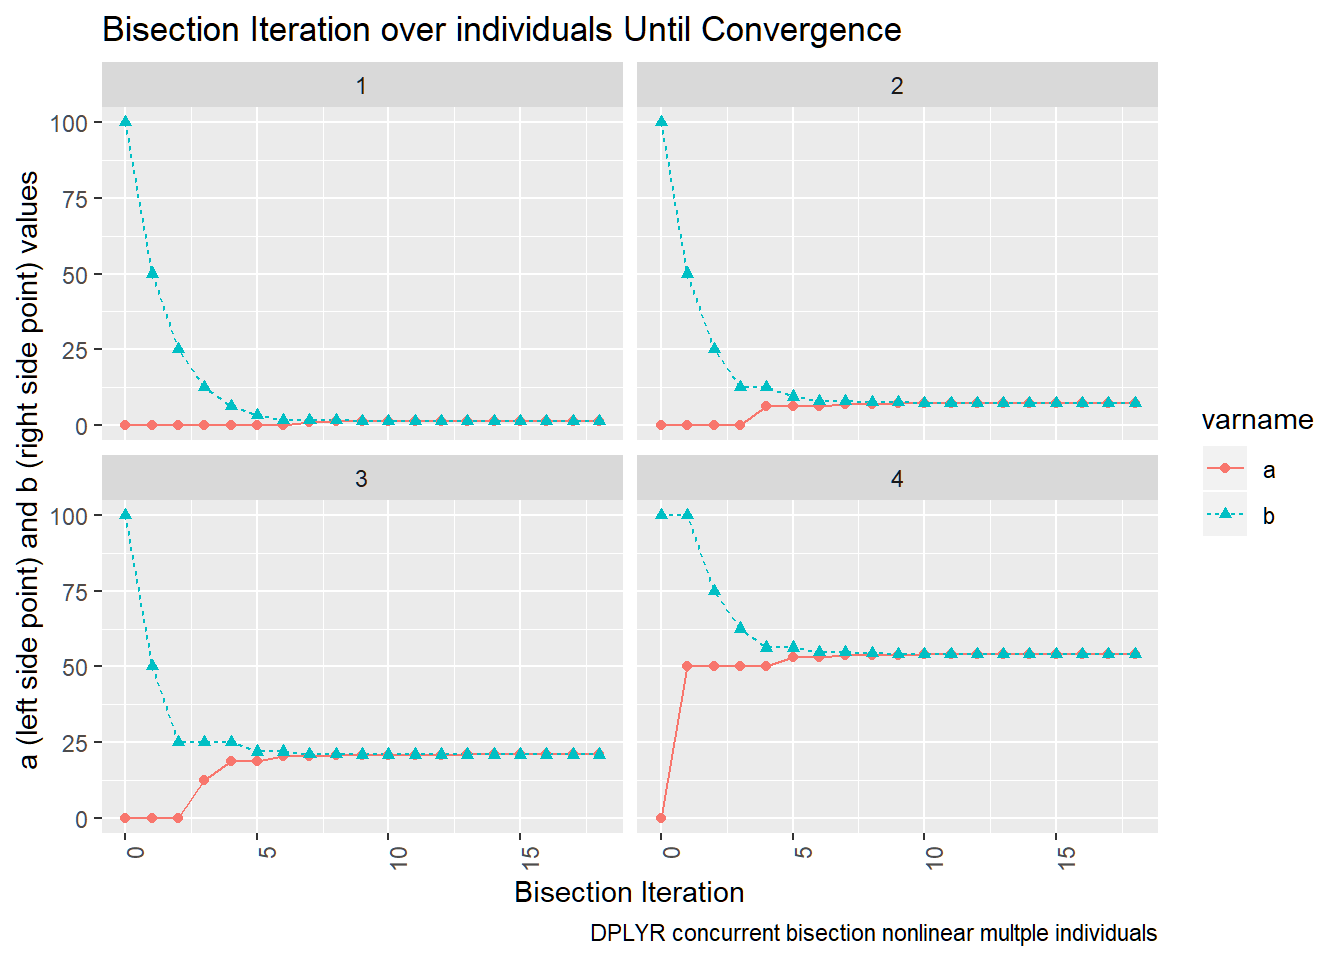
\includegraphics{Panel-Data-and-Optimization-with-R_files/figure-latex/reshape solution for graphing-1} \end{center}

\hypertarget{mathmatics-and-statistics}{%
\chapter{Mathmatics and Statistics}\label{mathmatics-and-statistics}}

\hypertarget{distributions}{%
\section{Distributions}\label{distributions}}

\hypertarget{integrate-over-normal-guassian-process-shock}{%
\subsection{Integrate Over Normal Guassian Process Shock}\label{integrate-over-normal-guassian-process-shock}}

\begin{quote}
Go back to \href{http://fanwangecon.github.io/}{fan}'s \href{https://fanwangecon.github.io/REconTools/}{REconTools} Package, \href{https://fanwangecon.github.io/R4Econ/}{R4Econ} Repository (\href{https://fanwangecon.github.io/R4Econ/bookdown}{bookdown site}), or \href{https://fanwangecon.github.io/Stat4Econ/}{Intro Stats with R} Repository.
\end{quote}

Some Common parameters

\begin{Shaded}
\begin{Highlighting}[]
\NormalTok{fl_eps_mean =}\StringTok{ }\DecValTok{10}
\NormalTok{fl_eps_sd =}\StringTok{ }\DecValTok{50}
\NormalTok{fl_cdf_min =}\StringTok{ }\FloatTok{0.000001}
\NormalTok{fl_cdf_max =}\StringTok{ }\FloatTok{0.999999}
\NormalTok{ar_it_draws <-}\StringTok{ }\KeywordTok{seq}\NormalTok{(}\DecValTok{1}\NormalTok{, }\DecValTok{1000}\NormalTok{)}
\end{Highlighting}
\end{Shaded}

\hypertarget{randomly-sample-and-integrate-monte-carlo-integration}{%
\subsubsection{Randomly Sample and Integrate (Monte Carlo integration)}\label{randomly-sample-and-integrate-monte-carlo-integration}}

Compare randomly drawn normal shock mean and known mean. How does simulated mean change with draws. Actual integral equals to \(10\), as sample size increases, the sample mean approaches the integration results, but this is expensive, even with ten thousand draws, not very exact.

\begin{Shaded}
\begin{Highlighting}[]
\CommentTok{# Simulate Draws}
\KeywordTok{set.seed}\NormalTok{(}\DecValTok{123}\NormalTok{)}
\NormalTok{ar_fl_means <-}
\StringTok{  }\KeywordTok{sapply}\NormalTok{(ar_it_draws, }\ControlFlowTok{function}\NormalTok{(x)}
    \KeywordTok{return}\NormalTok{(}\KeywordTok{mean}\NormalTok{(}\KeywordTok{rnorm}\NormalTok{(x[}\DecValTok{1}\NormalTok{], }\DataTypeTok{mean=}\NormalTok{fl_eps_mean, }\DataTypeTok{sd=}\NormalTok{fl_eps_sd))))}
\NormalTok{ar_fl_sd <-}
\StringTok{  }\KeywordTok{sapply}\NormalTok{(ar_it_draws, }\ControlFlowTok{function}\NormalTok{(x)}
    \KeywordTok{return}\NormalTok{(}\KeywordTok{sd}\NormalTok{(}\KeywordTok{rnorm}\NormalTok{(x[}\DecValTok{1}\NormalTok{], }\DataTypeTok{mean=}\NormalTok{fl_eps_mean, }\DataTypeTok{sd=}\NormalTok{fl_eps_sd))))}

\NormalTok{mt_sample_means <-}\StringTok{ }\KeywordTok{cbind}\NormalTok{(ar_it_draws, ar_fl_means, ar_fl_sd)}
\KeywordTok{colnames}\NormalTok{(mt_sample_means) <-}\StringTok{ }\KeywordTok{c}\NormalTok{(}\StringTok{'draw_count'}\NormalTok{, }\StringTok{'mean'}\NormalTok{, }\StringTok{'sd'}\NormalTok{)}
\NormalTok{tb_sample_means <-}\StringTok{ }\KeywordTok{as_tibble}\NormalTok{(mt_sample_means)}

\CommentTok{# Graph}
\CommentTok{# x-labels}
\NormalTok{x.labels <-}\StringTok{ }\KeywordTok{c}\NormalTok{(}\StringTok{'n=1'}\NormalTok{, }\StringTok{'n=10'}\NormalTok{, }\StringTok{'n=100'}\NormalTok{, }\StringTok{'n=1000'}\NormalTok{)}
\NormalTok{x.breaks <-}\StringTok{ }\KeywordTok{c}\NormalTok{(}\DecValTok{1}\NormalTok{, }\DecValTok{10}\NormalTok{, }\DecValTok{100}\NormalTok{, }\DecValTok{1000}\NormalTok{)}

\CommentTok{# Graph Results--Draw}
\NormalTok{plt_mean <-}\StringTok{ }\NormalTok{tb_sample_means }\OperatorTok
\StringTok{  }\KeywordTok{ggplot}\NormalTok{(}\KeywordTok{aes}\NormalTok{(}\DataTypeTok{x=}\NormalTok{draw_count, }\DataTypeTok{y=}\NormalTok{mean)) }\OperatorTok{+}
\StringTok{  }\KeywordTok{geom_line}\NormalTok{(}\DataTypeTok{size=}\FloatTok{0.75}\NormalTok{) }\OperatorTok{+}
\StringTok{  }\KeywordTok{labs}\NormalTok{(}\DataTypeTok{title =} \KeywordTok{paste0}\NormalTok{(}\StringTok{'Sample Average}
\StringTok{                      as Sample Size Increases}\CharTok{\textbackslash{}n}\StringTok{ True Mean='}\NormalTok{,}
\NormalTok{                      fl_eps_mean,}\StringTok{', sd='}\NormalTok{,fl_eps_sd),}
       \DataTypeTok{x =} \StringTok{'Sample Size'}\NormalTok{,}
       \DataTypeTok{y =} \StringTok{'Sample Mean'}\NormalTok{,}
       \DataTypeTok{caption =} \StringTok{'Mean of Sample Integrates to Mean'}\NormalTok{) }\OperatorTok{+}
\StringTok{  }\KeywordTok{scale_x_continuous}\NormalTok{(}\DataTypeTok{trans=}\StringTok{'log10'}\NormalTok{, }\DataTypeTok{labels =}\NormalTok{ x.labels, }\DataTypeTok{breaks =}\NormalTok{ x.breaks) }\OperatorTok{+}
\StringTok{  }\KeywordTok{theme_bw}\NormalTok{()}
\KeywordTok{print}\NormalTok{(plt_mean)}
\end{Highlighting}
\end{Shaded}

\begin{center}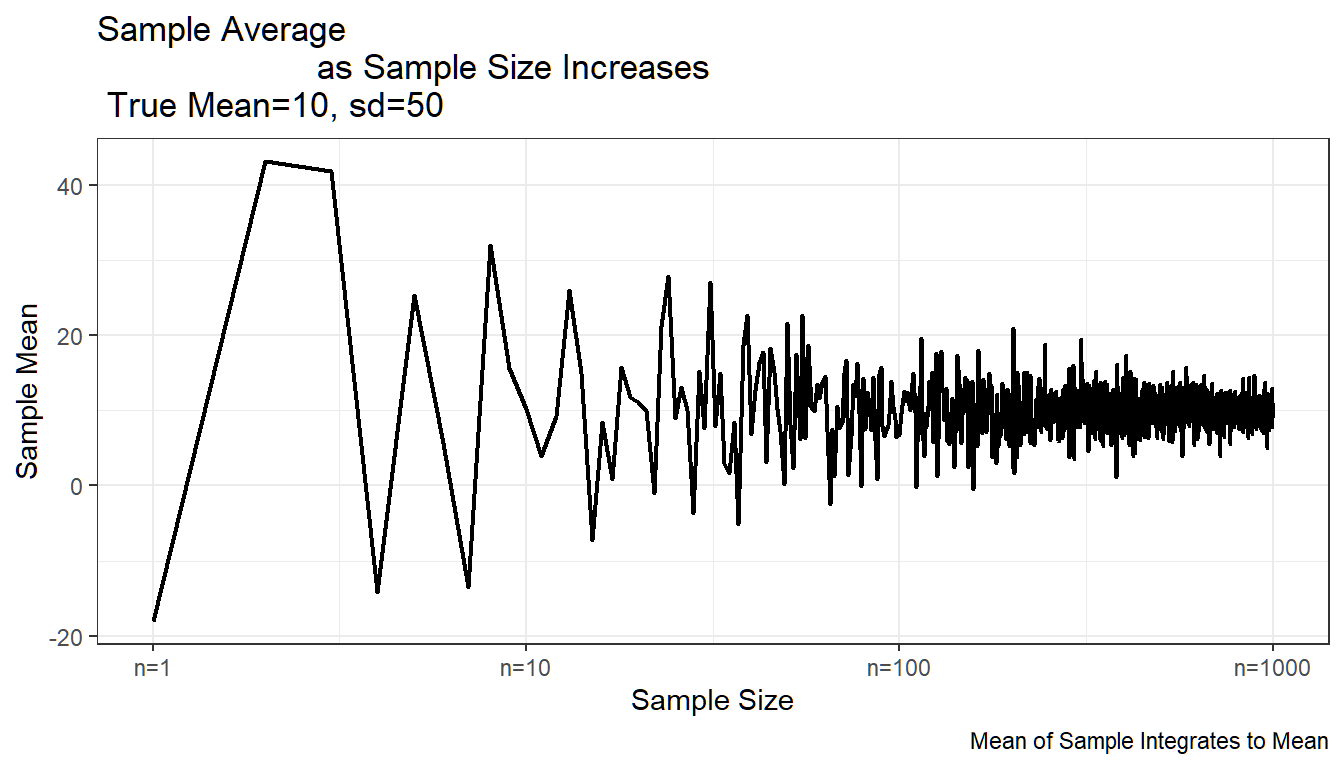
\includegraphics{Panel-Data-and-Optimization-with-R_files/figure-latex/unnamed-chunk-155-1} \end{center}

\begin{Shaded}
\begin{Highlighting}[]
\NormalTok{plt_sd <-}\StringTok{ }\NormalTok{tb_sample_means }\OperatorTok
\StringTok{  }\KeywordTok{ggplot}\NormalTok{(}\KeywordTok{aes}\NormalTok{(}\DataTypeTok{x=}\NormalTok{draw_count, }\DataTypeTok{y=}\NormalTok{sd)) }\OperatorTok{+}
\StringTok{  }\KeywordTok{geom_line}\NormalTok{(}\DataTypeTok{size=}\FloatTok{0.75}\NormalTok{) }\OperatorTok{+}
\StringTok{  }\KeywordTok{labs}\NormalTok{(}\DataTypeTok{title =} \KeywordTok{paste0}\NormalTok{(}\StringTok{'Sample Standard Deviation}
\StringTok{                      as Sample Size Increases}\CharTok{\textbackslash{}n}\StringTok{ True Mean='}\NormalTok{,}
\NormalTok{                      fl_eps_mean,}\StringTok{', sd='}\NormalTok{,fl_eps_sd),}
       \DataTypeTok{x =} \StringTok{'Sample Size'}\NormalTok{,}
       \DataTypeTok{y =} \StringTok{'Sample Standard Deviation'}\NormalTok{,}
       \DataTypeTok{caption =} \StringTok{'Standard Deviation of Sample Integrates to True Standard Deviation'}\NormalTok{) }\OperatorTok{+}
\StringTok{  }\KeywordTok{scale_x_continuous}\NormalTok{(}\DataTypeTok{trans=}\StringTok{'log10'}\NormalTok{, }\DataTypeTok{labels =}\NormalTok{ x.labels, }\DataTypeTok{breaks =}\NormalTok{ x.breaks) }\OperatorTok{+}
\StringTok{  }\KeywordTok{theme_bw}\NormalTok{()}
\KeywordTok{print}\NormalTok{(plt_sd)}
\end{Highlighting}
\end{Shaded}

\begin{verbatim}
## Warning: Removed 1 rows containing missing values (geom_path).
\end{verbatim}

\begin{center}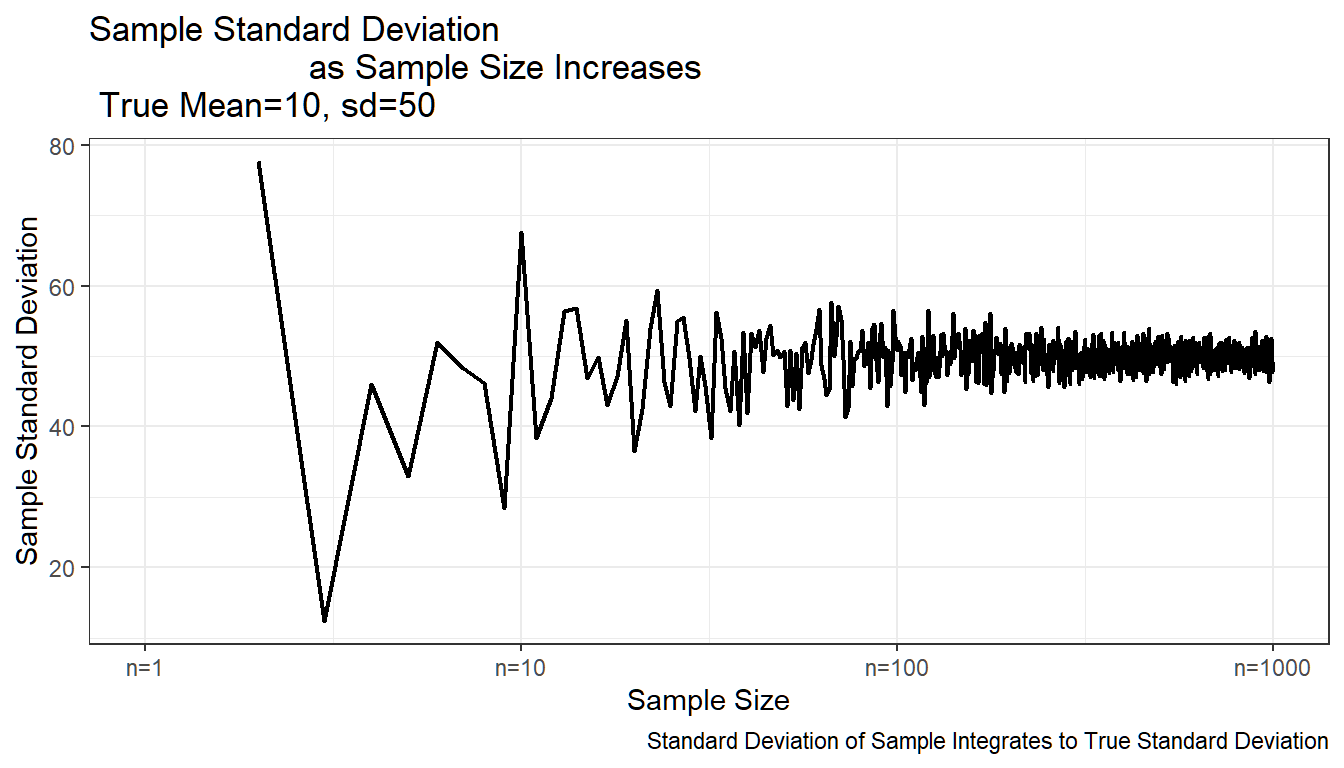
\includegraphics{Panel-Data-and-Optimization-with-R_files/figure-latex/unnamed-chunk-155-2} \end{center}

\hypertarget{integration-by-symmetric-uneven-rectangle}{%
\subsubsection{Integration By Symmetric Uneven Rectangle}\label{integration-by-symmetric-uneven-rectangle}}

Draw on grid from probability space, and then find use norm inverse to find corresponding x point. Under this approach, each rectangle is suppose to approximate the same same. So even area, but uneven width.

Resulting integration is rectangle based, but rectangle width differ. Th rectangle have wider width as they move away from the mean, and thin width close to the mean. This is much more stable than the random draw method, and approximates the true answer more accurately.

\begin{Shaded}
\begin{Highlighting}[]
\NormalTok{mt_fl_means <-}
\StringTok{  }\KeywordTok{sapply}\NormalTok{(ar_it_draws, }\ControlFlowTok{function}\NormalTok{(x) \{}

\NormalTok{    fl_prob_break =}\StringTok{ }\NormalTok{(fl_cdf_max }\OperatorTok{-}\StringTok{ }\NormalTok{fl_cdf_min)}\OperatorTok{/}\NormalTok{(x[}\DecValTok{1}\NormalTok{])}
\NormalTok{    ar_eps_bounds <-}\StringTok{ }\KeywordTok{qnorm}\NormalTok{(}\KeywordTok{seq}\NormalTok{(fl_cdf_min, fl_cdf_max,}
                               \DataTypeTok{by=}\NormalTok{(fl_cdf_max }\OperatorTok{-}\StringTok{ }\NormalTok{fl_cdf_min)}\OperatorTok{/}\NormalTok{(x[}\DecValTok{1}\NormalTok{])),}
                           \DataTypeTok{mean =}\NormalTok{ fl_eps_mean, }\DataTypeTok{sd =}\NormalTok{ fl_eps_sd)}
\NormalTok{    ar_eps_val <-}\StringTok{ }\NormalTok{(}\KeywordTok{tail}\NormalTok{(ar_eps_bounds, }\DecValTok{-1}\NormalTok{) }\OperatorTok{+}\StringTok{ }\KeywordTok{head}\NormalTok{(ar_eps_bounds, }\DecValTok{-1}\NormalTok{))}\OperatorTok{/}\DecValTok{2}
\NormalTok{    ar_eps_prb <-}\StringTok{ }\KeywordTok{rep}\NormalTok{(fl_prob_break}\OperatorTok{/}\NormalTok{(fl_cdf_max }\OperatorTok{-}\StringTok{ }\NormalTok{fl_cdf_min), x[}\DecValTok{1}\NormalTok{])}
\NormalTok{    ar_eps_fev <-}\StringTok{ }\KeywordTok{dnorm}\NormalTok{(ar_eps_val,}
                        \DataTypeTok{mean =}\NormalTok{ fl_eps_mean, }\DataTypeTok{sd =}\NormalTok{ fl_eps_sd)}

\NormalTok{    fl_cdf_total_approx <-}\StringTok{ }\KeywordTok{sum}\NormalTok{(ar_eps_fev}\OperatorTok{*}\KeywordTok{diff}\NormalTok{(ar_eps_bounds))}
\NormalTok{    fl_mean_approx <-}\StringTok{ }\KeywordTok{sum}\NormalTok{(ar_eps_val}\OperatorTok{*}\NormalTok{(ar_eps_fev}\OperatorTok{*}\KeywordTok{diff}\NormalTok{(ar_eps_bounds)))}
\NormalTok{    fl_sd_approx <-}\StringTok{ }\KeywordTok{sqrt}\NormalTok{(}\KeywordTok{sum}\NormalTok{((ar_eps_val}\OperatorTok{-}\NormalTok{fl_mean_approx)}\OperatorTok{^}\DecValTok{2}\OperatorTok{*}\NormalTok{(ar_eps_fev}\OperatorTok{*}\KeywordTok{diff}\NormalTok{(ar_eps_bounds))))}

    \KeywordTok{return}\NormalTok{(}\KeywordTok{list}\NormalTok{(}\DataTypeTok{cdf=}\NormalTok{fl_cdf_total_approx, }\DataTypeTok{mean=}\NormalTok{fl_mean_approx, }\DataTypeTok{sd=}\NormalTok{fl_sd_approx))}
\NormalTok{  \})}

\NormalTok{mt_sample_means <-}\StringTok{ }\KeywordTok{cbind}\NormalTok{(ar_it_draws, }\KeywordTok{as_tibble}\NormalTok{(}\KeywordTok{t}\NormalTok{(mt_fl_means)) }\OperatorTok\StringTok{ }\KeywordTok{unnest}\NormalTok{())}
\end{Highlighting}
\end{Shaded}

\begin{verbatim}
## Warning: `cols` is now required.
## Please use `cols = c(cdf, mean, sd)`
\end{verbatim}

\begin{Shaded}
\begin{Highlighting}[]
\KeywordTok{colnames}\NormalTok{(mt_sample_means) <-}\StringTok{ }\KeywordTok{c}\NormalTok{(}\StringTok{'draw_count'}\NormalTok{, }\StringTok{'cdf'}\NormalTok{, }\StringTok{'mean'}\NormalTok{, }\StringTok{'sd'}\NormalTok{)}
\NormalTok{tb_sample_means <-}\StringTok{ }\KeywordTok{as_tibble}\NormalTok{(mt_sample_means)}

\CommentTok{# Graph}
\CommentTok{# x-labels}
\NormalTok{x.labels <-}\StringTok{ }\KeywordTok{c}\NormalTok{(}\StringTok{'n=1'}\NormalTok{, }\StringTok{'n=10'}\NormalTok{, }\StringTok{'n=100'}\NormalTok{, }\StringTok{'n=1000'}\NormalTok{)}
\NormalTok{x.breaks <-}\StringTok{ }\KeywordTok{c}\NormalTok{(}\DecValTok{1}\NormalTok{, }\DecValTok{10}\NormalTok{, }\DecValTok{100}\NormalTok{, }\DecValTok{1000}\NormalTok{)}

\CommentTok{# Graph Results--Draw}
\NormalTok{plt_mean <-}\StringTok{ }\NormalTok{tb_sample_means }\OperatorTok
\StringTok{  }\KeywordTok{ggplot}\NormalTok{(}\KeywordTok{aes}\NormalTok{(}\DataTypeTok{x=}\NormalTok{draw_count, }\DataTypeTok{y=}\NormalTok{mean)) }\OperatorTok{+}
\StringTok{  }\KeywordTok{geom_line}\NormalTok{(}\DataTypeTok{size=}\FloatTok{0.75}\NormalTok{) }\OperatorTok{+}
\StringTok{  }\KeywordTok{labs}\NormalTok{(}\DataTypeTok{title =} \KeywordTok{paste0}\NormalTok{(}\StringTok{'Average as Uneven Rectangle}
\StringTok{                      Count Increases}\CharTok{\textbackslash{}n}\StringTok{ True Mean='}\NormalTok{,}
\NormalTok{                      fl_eps_mean,}\StringTok{', sd='}\NormalTok{,fl_eps_sd),}
       \DataTypeTok{x =} \StringTok{'Number of Uneven Rectangles for Approximation'}\NormalTok{,}
       \DataTypeTok{y =} \StringTok{'Integrated Mean'}\NormalTok{,}
       \DataTypeTok{caption =} \StringTok{'Integral Approximation as Uneven Rectangle Count Increases'}\NormalTok{) }\OperatorTok{+}
\StringTok{  }\KeywordTok{scale_x_continuous}\NormalTok{(}\DataTypeTok{trans=}\StringTok{'log10'}\NormalTok{, }\DataTypeTok{labels =}\NormalTok{ x.labels, }\DataTypeTok{breaks =}\NormalTok{ x.breaks) }\OperatorTok{+}
\StringTok{  }\KeywordTok{theme_bw}\NormalTok{()}
\KeywordTok{print}\NormalTok{(plt_mean)}
\end{Highlighting}
\end{Shaded}

\begin{center}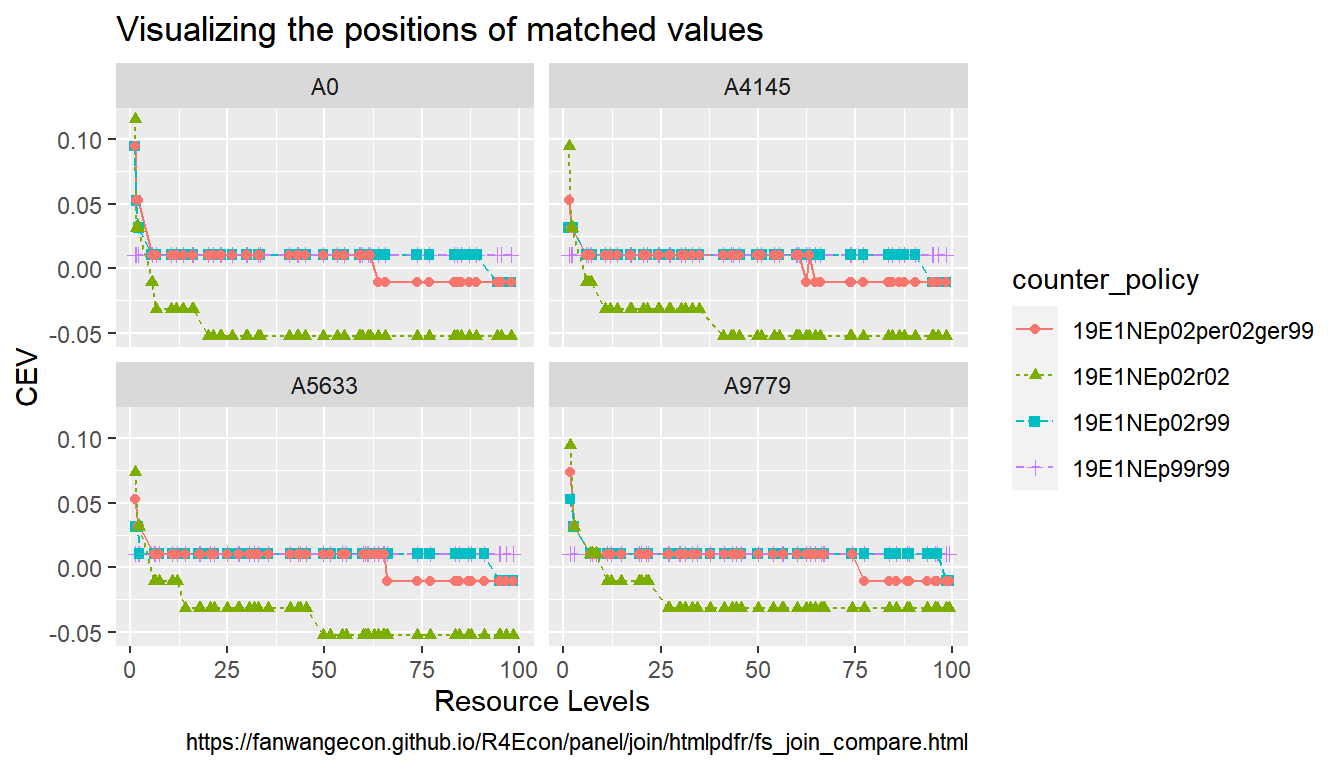
\includegraphics{Panel-Data-and-Optimization-with-R_files/figure-latex/unnamed-chunk-156-1} \end{center}

\begin{Shaded}
\begin{Highlighting}[]
\NormalTok{plt_sd <-}\StringTok{ }\NormalTok{tb_sample_means }\OperatorTok
\StringTok{  }\KeywordTok{ggplot}\NormalTok{(}\KeywordTok{aes}\NormalTok{(}\DataTypeTok{x=}\NormalTok{draw_count, }\DataTypeTok{y=}\NormalTok{sd)) }\OperatorTok{+}
\StringTok{  }\KeywordTok{geom_line}\NormalTok{(}\DataTypeTok{size=}\FloatTok{0.75}\NormalTok{) }\OperatorTok{+}
\StringTok{  }\KeywordTok{labs}\NormalTok{(}\DataTypeTok{title =} \KeywordTok{paste0}\NormalTok{(}\StringTok{'Standard Deviation as Uneven Rectangle}
\StringTok{                      Count Increases}\CharTok{\textbackslash{}n}\StringTok{ True Mean='}\NormalTok{,}
\NormalTok{                      fl_eps_mean,}\StringTok{', sd='}\NormalTok{,fl_eps_sd),}
       \DataTypeTok{x =} \StringTok{'Number of Uneven Rectangles for Approximation'}\NormalTok{,}
       \DataTypeTok{y =} \StringTok{'Standard Deviation'}\NormalTok{,}
       \DataTypeTok{caption =} \StringTok{'Integral Approximation as Uneven Rectangle Count Increases'}\NormalTok{) }\OperatorTok{+}
\StringTok{  }\KeywordTok{scale_x_continuous}\NormalTok{(}\DataTypeTok{trans=}\StringTok{'log10'}\NormalTok{, }\DataTypeTok{labels =}\NormalTok{ x.labels, }\DataTypeTok{breaks =}\NormalTok{ x.breaks) }\OperatorTok{+}
\StringTok{  }\KeywordTok{theme_bw}\NormalTok{()}
\KeywordTok{print}\NormalTok{(plt_sd)}
\end{Highlighting}
\end{Shaded}

\begin{center}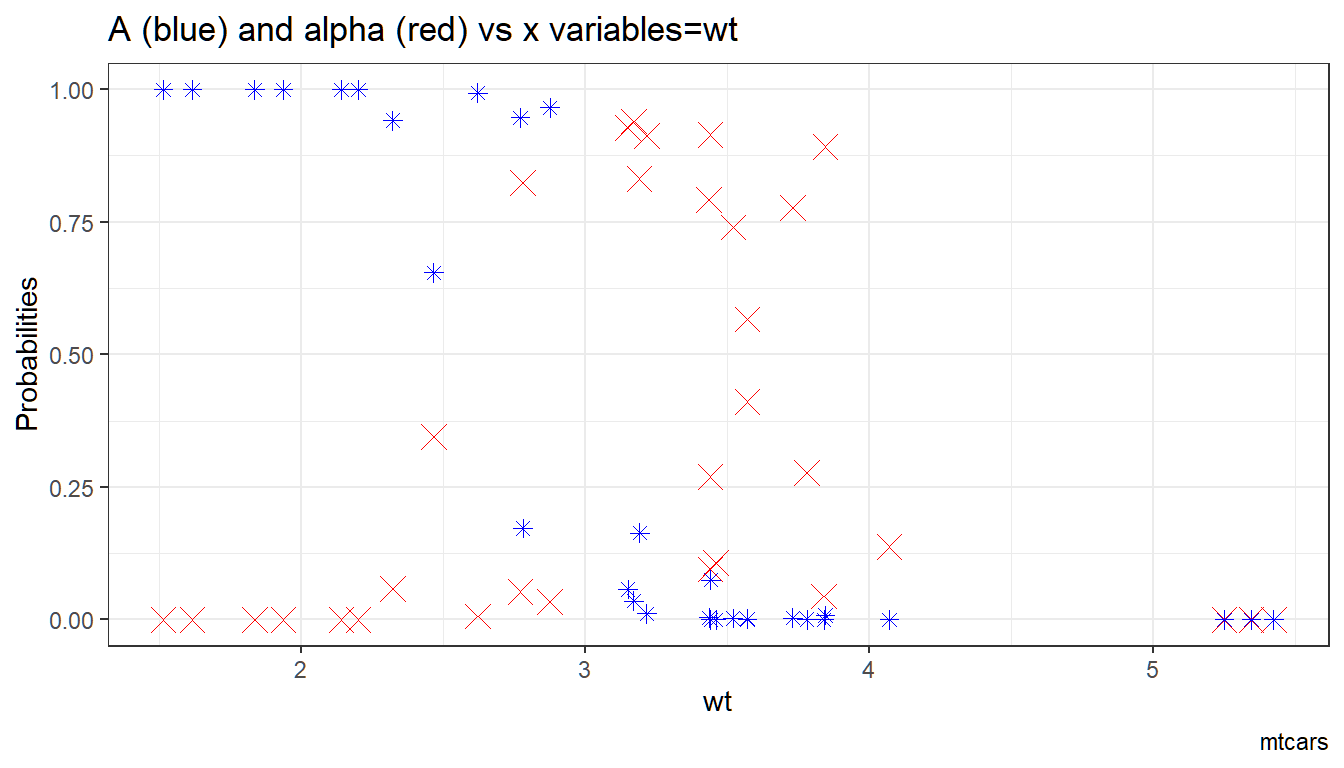
\includegraphics{Panel-Data-and-Optimization-with-R_files/figure-latex/unnamed-chunk-156-2} \end{center}

\begin{Shaded}
\begin{Highlighting}[]
\NormalTok{plt_cdf <-}\StringTok{ }\NormalTok{tb_sample_means }\OperatorTok
\StringTok{  }\KeywordTok{ggplot}\NormalTok{(}\KeywordTok{aes}\NormalTok{(}\DataTypeTok{x=}\NormalTok{draw_count, }\DataTypeTok{y=}\NormalTok{cdf)) }\OperatorTok{+}
\StringTok{  }\KeywordTok{geom_line}\NormalTok{(}\DataTypeTok{size=}\FloatTok{0.75}\NormalTok{) }\OperatorTok{+}
\StringTok{  }\KeywordTok{labs}\NormalTok{(}\DataTypeTok{title =} \KeywordTok{paste0}\NormalTok{(}\StringTok{'Aggregate Probability as Uneven Rectangle}
\StringTok{                      Count Increases}\CharTok{\textbackslash{}n}\StringTok{ True Mean='}\NormalTok{,}
\NormalTok{                      fl_eps_mean,}\StringTok{', sd='}\NormalTok{,fl_eps_sd),}
       \DataTypeTok{x =} \StringTok{'Number of Uneven Rectangles for Approximation'}\NormalTok{,}
       \DataTypeTok{y =} \StringTok{'Aggregate Probability'}\NormalTok{,}
       \DataTypeTok{caption =} \StringTok{'Aggregate Probability Approximation as Uneven Rectangle Count Increases'}\NormalTok{) }\OperatorTok{+}
\StringTok{  }\KeywordTok{scale_x_continuous}\NormalTok{(}\DataTypeTok{trans=}\StringTok{'log10'}\NormalTok{, }\DataTypeTok{labels =}\NormalTok{ x.labels, }\DataTypeTok{breaks =}\NormalTok{ x.breaks) }\OperatorTok{+}
\StringTok{  }\KeywordTok{theme_bw}\NormalTok{()}
\KeywordTok{print}\NormalTok{(plt_cdf)}
\end{Highlighting}
\end{Shaded}

\begin{center}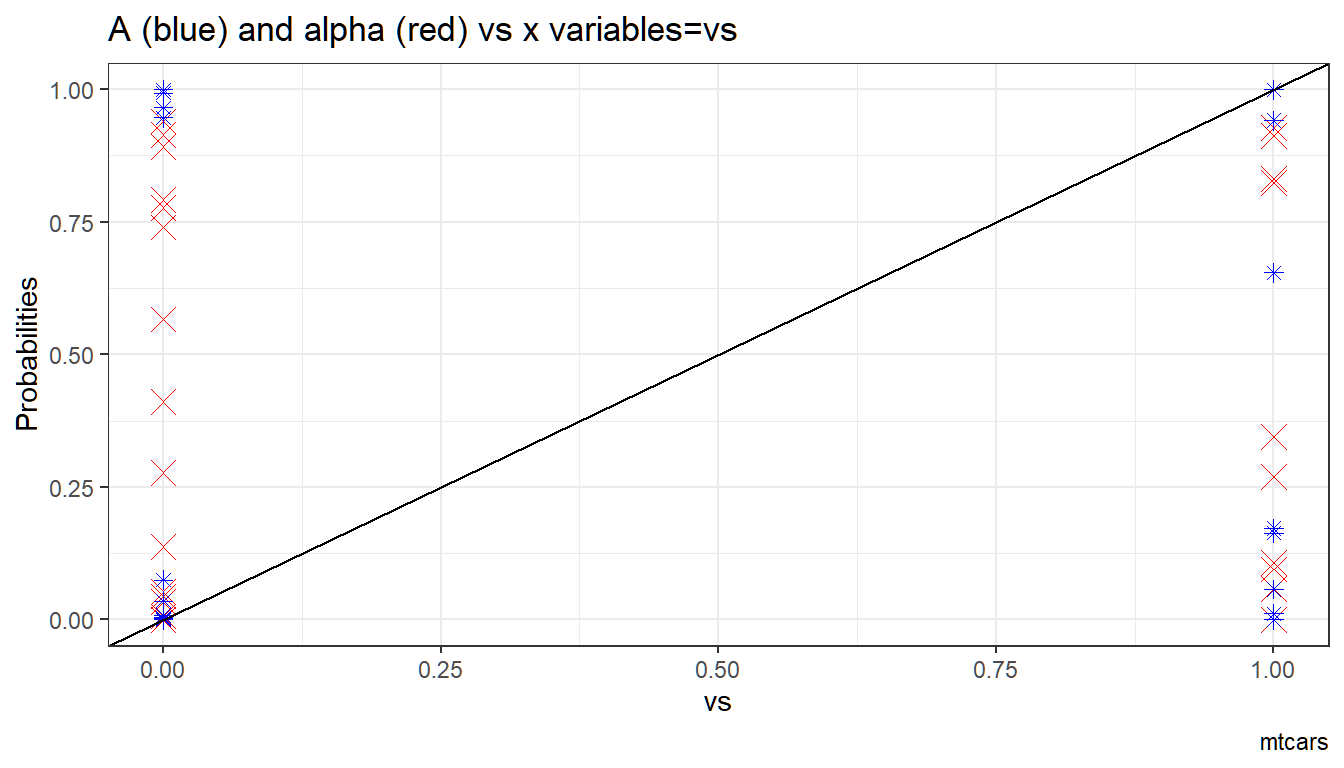
\includegraphics{Panel-Data-and-Optimization-with-R_files/figure-latex/unnamed-chunk-156-3} \end{center}

\hypertarget{integration-by-constant-width-rectangle-trapezoidal-rule}{%
\subsubsection{Integration By Constant Width Rectangle (Trapezoidal rule)}\label{integration-by-constant-width-rectangle-trapezoidal-rule}}

This is implementing even width recentagle, even along x-axis take points, and measure \(f(x)\). Rectangle width are the same. This is even width, but uneven area. Note that this method approximates the true answer much better and more quickly.

\begin{Shaded}
\begin{Highlighting}[]
\NormalTok{mt_fl_means <-}
\StringTok{  }\KeywordTok{sapply}\NormalTok{(ar_it_draws, }\ControlFlowTok{function}\NormalTok{(x) \{}

\NormalTok{    fl_eps_min <-}\StringTok{ }\KeywordTok{qnorm}\NormalTok{(fl_cdf_min, }\DataTypeTok{mean =}\NormalTok{ fl_eps_mean, }\DataTypeTok{sd =}\NormalTok{ fl_eps_sd)}
\NormalTok{    fl_eps_max <-}\StringTok{ }\KeywordTok{qnorm}\NormalTok{(fl_cdf_max, }\DataTypeTok{mean =}\NormalTok{ fl_eps_mean, }\DataTypeTok{sd =}\NormalTok{ fl_eps_sd)}
\NormalTok{    fl_gap <-}\StringTok{ }\NormalTok{(fl_eps_max}\OperatorTok{-}\NormalTok{fl_eps_min)}\OperatorTok{/}\NormalTok{(x[}\DecValTok{1}\NormalTok{])}
\NormalTok{    ar_eps_bounds <-}\StringTok{ }\KeywordTok{seq}\NormalTok{(fl_eps_min, fl_eps_max, }\DataTypeTok{by=}\NormalTok{fl_gap)}
\NormalTok{    ar_eps_val <-}\StringTok{ }\NormalTok{(}\KeywordTok{tail}\NormalTok{(ar_eps_bounds, }\DecValTok{-1}\NormalTok{) }\OperatorTok{+}\StringTok{ }\KeywordTok{head}\NormalTok{(ar_eps_bounds, }\DecValTok{-1}\NormalTok{))}\OperatorTok{/}\DecValTok{2}
\NormalTok{    ar_eps_prb <-}\StringTok{ }\KeywordTok{dnorm}\NormalTok{(ar_eps_val, }\DataTypeTok{mean =}\NormalTok{ fl_eps_mean, }\DataTypeTok{sd =}\NormalTok{ fl_eps_sd)}\OperatorTok{*}\NormalTok{fl_gap}

\NormalTok{    fl_cdf_total_approx <-}\StringTok{ }\KeywordTok{sum}\NormalTok{(ar_eps_prb)}
\NormalTok{    fl_mean_approx <-}\StringTok{ }\KeywordTok{sum}\NormalTok{(ar_eps_val}\OperatorTok{*}\NormalTok{ar_eps_prb)}
\NormalTok{    fl_sd_approx <-}\StringTok{ }\KeywordTok{sqrt}\NormalTok{(}\KeywordTok{sum}\NormalTok{((ar_eps_val}\OperatorTok{-}\NormalTok{fl_mean_approx)}\OperatorTok{^}\DecValTok{2}\OperatorTok{*}\NormalTok{ar_eps_prb))}

    \KeywordTok{return}\NormalTok{(}\KeywordTok{list}\NormalTok{(}\DataTypeTok{cdf=}\NormalTok{fl_cdf_total_approx, }\DataTypeTok{mean=}\NormalTok{fl_mean_approx, }\DataTypeTok{sd=}\NormalTok{fl_sd_approx))}
\NormalTok{  \})}

\NormalTok{mt_sample_means <-}\StringTok{ }\KeywordTok{cbind}\NormalTok{(ar_it_draws, }\KeywordTok{as_tibble}\NormalTok{(}\KeywordTok{t}\NormalTok{(mt_fl_means)) }\OperatorTok\StringTok{ }\KeywordTok{unnest}\NormalTok{())}
\end{Highlighting}
\end{Shaded}

\begin{verbatim}
## Warning: `cols` is now required.
## Please use `cols = c(cdf, mean, sd)`
\end{verbatim}

\begin{Shaded}
\begin{Highlighting}[]
\KeywordTok{colnames}\NormalTok{(mt_sample_means) <-}\StringTok{ }\KeywordTok{c}\NormalTok{(}\StringTok{'draw_count'}\NormalTok{, }\StringTok{'cdf'}\NormalTok{, }\StringTok{'mean'}\NormalTok{, }\StringTok{'sd'}\NormalTok{)}
\NormalTok{tb_sample_means <-}\StringTok{ }\KeywordTok{as_tibble}\NormalTok{(mt_sample_means)}

\CommentTok{# Graph}
\CommentTok{# x-labels}
\NormalTok{x.labels <-}\StringTok{ }\KeywordTok{c}\NormalTok{(}\StringTok{'n=1'}\NormalTok{, }\StringTok{'n=10'}\NormalTok{, }\StringTok{'n=100'}\NormalTok{, }\StringTok{'n=1000'}\NormalTok{)}
\NormalTok{x.breaks <-}\StringTok{ }\KeywordTok{c}\NormalTok{(}\DecValTok{1}\NormalTok{, }\DecValTok{10}\NormalTok{, }\DecValTok{100}\NormalTok{, }\DecValTok{1000}\NormalTok{)}

\CommentTok{# Graph Results--Draw}
\NormalTok{plt_mean <-}\StringTok{ }\NormalTok{tb_sample_means }\OperatorTok
\StringTok{  }\KeywordTok{ggplot}\NormalTok{(}\KeywordTok{aes}\NormalTok{(}\DataTypeTok{x=}\NormalTok{draw_count, }\DataTypeTok{y=}\NormalTok{mean)) }\OperatorTok{+}
\StringTok{  }\KeywordTok{geom_line}\NormalTok{(}\DataTypeTok{size=}\FloatTok{0.75}\NormalTok{) }\OperatorTok{+}
\StringTok{  }\KeywordTok{labs}\NormalTok{(}\DataTypeTok{title =} \KeywordTok{paste0}\NormalTok{(}\StringTok{'Average as Even Rectangle}
\StringTok{                      Count Increases}\CharTok{\textbackslash{}n}\StringTok{ True Mean='}\NormalTok{,}
\NormalTok{                      fl_eps_mean,}\StringTok{', sd='}\NormalTok{,fl_eps_sd),}
       \DataTypeTok{x =} \StringTok{'Number of Even Rectangles for Approximation'}\NormalTok{,}
       \DataTypeTok{y =} \StringTok{'Integrated Mean'}\NormalTok{,}
       \DataTypeTok{caption =} \StringTok{'Integral Approximation as Even Rectangle Count Increases'}\NormalTok{) }\OperatorTok{+}
\StringTok{  }\KeywordTok{scale_x_continuous}\NormalTok{(}\DataTypeTok{trans=}\StringTok{'log10'}\NormalTok{, }\DataTypeTok{labels =}\NormalTok{ x.labels, }\DataTypeTok{breaks =}\NormalTok{ x.breaks) }\OperatorTok{+}
\StringTok{  }\KeywordTok{theme_bw}\NormalTok{()}
\KeywordTok{print}\NormalTok{(plt_mean)}
\end{Highlighting}
\end{Shaded}

\begin{center}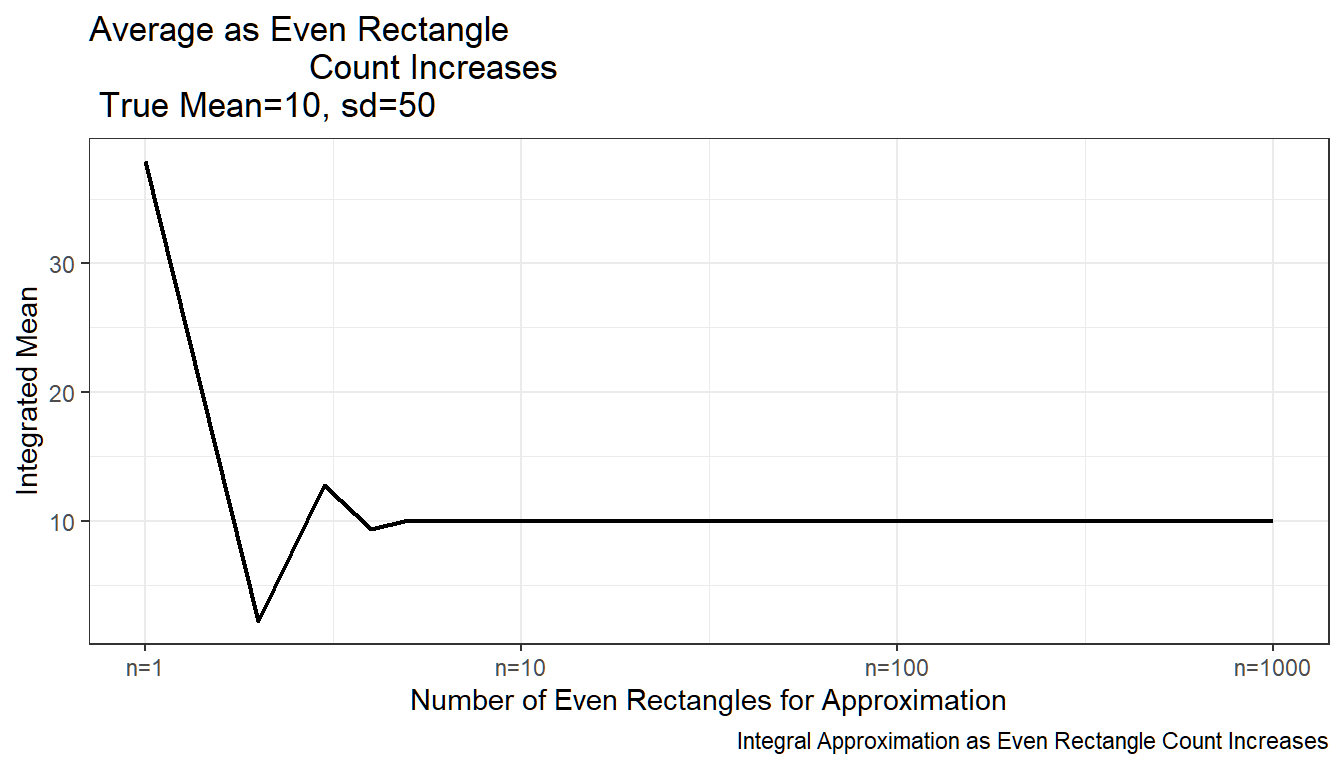
\includegraphics{Panel-Data-and-Optimization-with-R_files/figure-latex/unnamed-chunk-157-1} \end{center}

\begin{Shaded}
\begin{Highlighting}[]
\NormalTok{plt_sd <-}\StringTok{ }\NormalTok{tb_sample_means }\OperatorTok
\StringTok{  }\KeywordTok{ggplot}\NormalTok{(}\KeywordTok{aes}\NormalTok{(}\DataTypeTok{x=}\NormalTok{draw_count, }\DataTypeTok{y=}\NormalTok{sd)) }\OperatorTok{+}
\StringTok{  }\KeywordTok{geom_line}\NormalTok{(}\DataTypeTok{size=}\FloatTok{0.75}\NormalTok{) }\OperatorTok{+}
\StringTok{  }\KeywordTok{labs}\NormalTok{(}\DataTypeTok{title =} \KeywordTok{paste0}\NormalTok{(}\StringTok{'Standard Deviation as Even Rectangle}
\StringTok{                      Count Increases}\CharTok{\textbackslash{}n}\StringTok{ True Mean='}\NormalTok{,}
\NormalTok{                      fl_eps_mean,}\StringTok{', sd='}\NormalTok{,fl_eps_sd),}
       \DataTypeTok{x =} \StringTok{'Number of Even Rectangles for Approximation'}\NormalTok{,}
       \DataTypeTok{y =} \StringTok{'Standard Deviation'}\NormalTok{,}
       \DataTypeTok{caption =} \StringTok{'Integral Approximation as Even Rectangle Count Increases'}\NormalTok{) }\OperatorTok{+}
\StringTok{  }\KeywordTok{scale_x_continuous}\NormalTok{(}\DataTypeTok{trans=}\StringTok{'log10'}\NormalTok{, }\DataTypeTok{labels =}\NormalTok{ x.labels, }\DataTypeTok{breaks =}\NormalTok{ x.breaks) }\OperatorTok{+}
\StringTok{  }\KeywordTok{theme_bw}\NormalTok{()}
\KeywordTok{print}\NormalTok{(plt_sd)}
\end{Highlighting}
\end{Shaded}

\begin{center}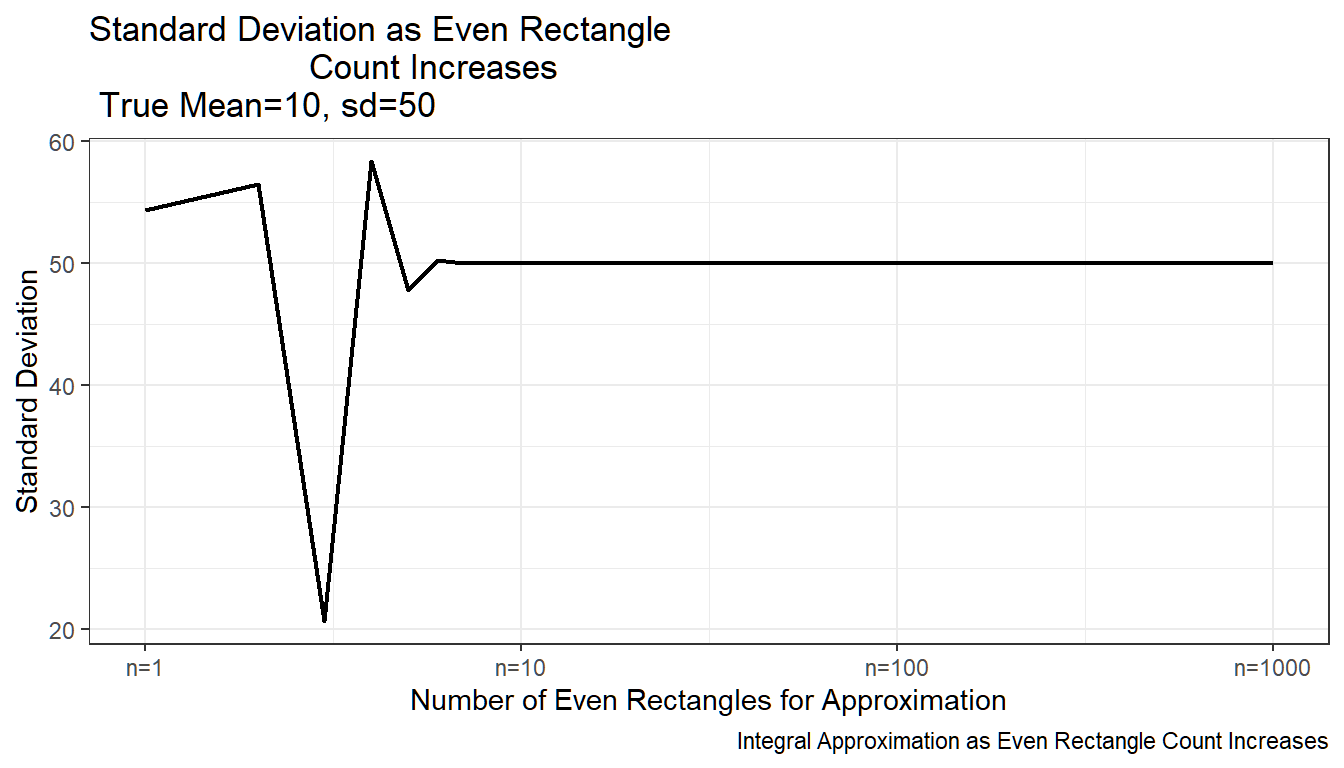
\includegraphics{Panel-Data-and-Optimization-with-R_files/figure-latex/unnamed-chunk-157-2} \end{center}

\begin{Shaded}
\begin{Highlighting}[]
\NormalTok{plt_cdf <-}\StringTok{ }\NormalTok{tb_sample_means }\OperatorTok
\StringTok{  }\KeywordTok{ggplot}\NormalTok{(}\KeywordTok{aes}\NormalTok{(}\DataTypeTok{x=}\NormalTok{draw_count, }\DataTypeTok{y=}\NormalTok{cdf)) }\OperatorTok{+}
\StringTok{  }\KeywordTok{geom_line}\NormalTok{(}\DataTypeTok{size=}\FloatTok{0.75}\NormalTok{) }\OperatorTok{+}
\StringTok{  }\KeywordTok{labs}\NormalTok{(}\DataTypeTok{title =} \KeywordTok{paste0}\NormalTok{(}\StringTok{'Aggregate Probability as Even Rectangle}
\StringTok{                      Count Increases}\CharTok{\textbackslash{}n}\StringTok{ True Mean='}\NormalTok{,}
\NormalTok{                      fl_eps_mean,}\StringTok{', sd='}\NormalTok{,fl_eps_sd),}
       \DataTypeTok{x =} \StringTok{'Number of Even Rectangles for Approximation'}\NormalTok{,}
       \DataTypeTok{y =} \StringTok{'Aggregate Probability'}\NormalTok{,}
       \DataTypeTok{caption =} \StringTok{'Aggregate Probability Approximation as Even Rectangle Count Increases'}\NormalTok{) }\OperatorTok{+}
\StringTok{  }\KeywordTok{scale_x_continuous}\NormalTok{(}\DataTypeTok{trans=}\StringTok{'log10'}\NormalTok{, }\DataTypeTok{labels =}\NormalTok{ x.labels, }\DataTypeTok{breaks =}\NormalTok{ x.breaks) }\OperatorTok{+}
\StringTok{  }\KeywordTok{theme_bw}\NormalTok{()}
\KeywordTok{print}\NormalTok{(plt_cdf)}
\end{Highlighting}
\end{Shaded}

\begin{center}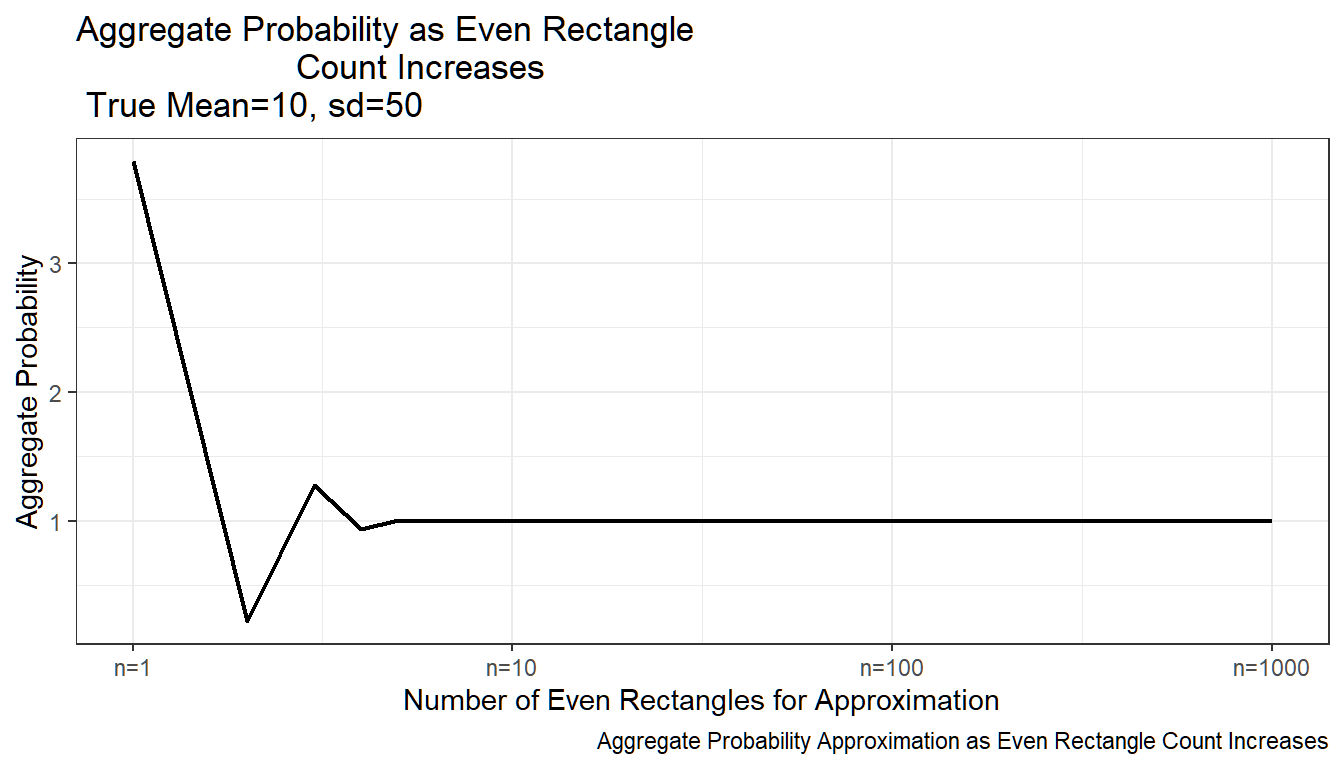
\includegraphics{Panel-Data-and-Optimization-with-R_files/figure-latex/unnamed-chunk-157-3} \end{center}

\hypertarget{analytical-solutions}{%
\section{Analytical Solutions}\label{analytical-solutions}}

\hypertarget{linear-scalar-fx0-solutions}{%
\subsection{Linear Scalar f(x)=0 Solutions}\label{linear-scalar-fx0-solutions}}

\begin{quote}
Go back to \href{http://fanwangecon.github.io/}{fan}'s \href{https://fanwangecon.github.io/REconTools/}{REconTools} Package, \href{https://fanwangecon.github.io/R4Econ/}{R4Econ} Repository (\href{https://fanwangecon.github.io/R4Econ/bookdown}{bookdown site}), or \href{https://fanwangecon.github.io/Stat4Econ/}{Intro Stats with R} Repository.
\end{quote}

\hypertarget{ratio}{%
\subsubsection{Ratio}\label{ratio}}

Here are some common ratios.

\hypertarget{unif-draw-min-and-max-ratio}{%
\paragraph{Unif Draw Min and Max Ratio}\label{unif-draw-min-and-max-ratio}}

We want to draw numbers such that we have some mean \(b\), and that the possible maximum and minimum value drawn are at most \(a\) times apart. Given \(b\) and \(a\), solve for \(x\).

\[
f(x) = \frac{b+x}{b-x} - a = 0
\]

\[
b \cdot a - x \cdot a = b + x \\
b \cdot a - b = x + x \cdot a  \\
b \left(a - 1\right) = x \left( a+ 1\right)  \\
x = \frac{b\left(a-1\right)}{a+1}\\
\]

Uniformly draw

\begin{Shaded}
\begin{Highlighting}[]
\NormalTok{b <-}\StringTok{ }\DecValTok{100}
\NormalTok{a <-}\StringTok{ }\DecValTok{2}
\NormalTok{x <-}\StringTok{ }\NormalTok{(b}\OperatorTok{*}\NormalTok{(a}\DecValTok{-1}\NormalTok{))}\OperatorTok{/}\NormalTok{(a}\OperatorTok{+}\DecValTok{1}\NormalTok{)}
\NormalTok{ar_unif_draws <-}\StringTok{ }\KeywordTok{runif}\NormalTok{(}\DecValTok{100}\NormalTok{, }\DataTypeTok{min=}\NormalTok{b}\OperatorTok{-}\NormalTok{x, }\DataTypeTok{max=}\NormalTok{b}\OperatorTok{+}\NormalTok{x)}
\NormalTok{fl_max_min_ratio <-}\StringTok{ }\KeywordTok{max}\NormalTok{(ar_unif_draws)}\OperatorTok{/}\KeywordTok{min}\NormalTok{(ar_unif_draws)}
\KeywordTok{cat}\NormalTok{(}\StringTok{'fl_max_min_ratio ='}\NormalTok{, fl_max_min_ratio, }\StringTok{'is close to a ='}\NormalTok{, a, }\StringTok{'}\CharTok{\textbackslash{}n}\StringTok{'}\NormalTok{)}
\end{Highlighting}
\end{Shaded}

\begin{verbatim}
## fl_max_min_ratio = 1.965882 is close to a = 2
\end{verbatim}

\hypertarget{inequality-models}{%
\section{Inequality Models}\label{inequality-models}}

\hypertarget{gini-discrete-sample}{%
\subsection{Gini Discrete Sample}\label{gini-discrete-sample}}

\begin{quote}
Go back to \href{http://fanwangecon.github.io/}{fan}'s \href{https://fanwangecon.github.io/REconTools/}{REconTools} Package, \href{https://fanwangecon.github.io/R4Econ/}{R4Econ} Repository (\href{https://fanwangecon.github.io/R4Econ/bookdown}{bookdown site}), or \href{https://fanwangecon.github.io/Stat4Econ/}{Intro Stats with R} Repository.
\end{quote}

This works out how the \href{https://fanwangecon.github.io/REconTools/reference/ff_dist_gini_vector_pos.html}{ff\_dist\_gini\_vector\_pos} function works from \href{https://fanwangecon.github.io/}{Fan}'s \emph{\href{https://fanwangecon.github.io/REconTools/}{REconTools}} Package.

\hypertarget{gini-formula-for-discrete-sample}{%
\subsubsection{Gini Formula for Discrete Sample}\label{gini-formula-for-discrete-sample}}

There is an vector values (all positive). This could be height information for N individuals. It could also be income information for N individuals. Calculate the \href{https://en.wikipedia.org/wiki/Gini_coefficient}{GINI} coefficient treating the given vector as population. This is not an estimation exercise where we want to estimate population gini based on a sample. The given array is the population. The population is discrete, and only has these N individuals in the length n vector.

Note that when the sample size is small, there is a limit to inequality using the formula defined below given each \(N\). So for small \(N\), can not really compare inequality across arrays with different \(N\), can only compare arrays with the same \(N\). In another word, if 1 of N individual holds all resource, as \(N\) increases, GINI will asymptote to 1, but it is very far away from 1 for low N.

The GINI formula used here is:
\[
 GINI =
  1 - \frac{2}{N+1}
  \cdot
  \left(\sum_{i=1}^N \sum_{j=1}^{i} x_j\right)
  \cdot
  \left(
    \sum_{i=1}^N x_i
  \right)^{-1}
\]

Derive the formula in the steps below.

\emph{Step 1 Area Formula}

\[
 \Gamma = \sum_{i=1}^N \frac{1}{N} \cdot \left(
     \sum_{j=1}^{i} \left(
      \frac{x_j}{\sum_{\widehat{j}=1}^N x_{\widehat{j}} }
      \right)
  \right)
\]

\emph{Step 2 Total Area Given Perfect equality}

With perfect equality \(x_i=a\) for all \(i\), so need to divide by that.

\[
 \Gamma^{\text{equal}} = \sum_{i=1}^N \frac{1}{N} \cdot \left(
     \sum_{j=1}^{i} \left(
      \frac{a}{\sum_{\widehat{j}=1}^N a }
      \right)
  \right)
  = \frac{N+1}{N}\cdot\frac{1}{2}
\]

As the number of elements of the vecotr increases:
\[
 \lim_{N \rightarrow \infty}\Gamma^{\text{equal}}
  = \lim_{N \rightarrow \infty} \frac{N+1}{N}\cdot\frac{1}{2}
  = \frac{1}{2}
\]

\emph{Step 3 Arriving at Finite Vector Gini Formula}

Given what we have from above, we obtain the gini formula, divide by total area below 45 degree line.

\[
 GINI =
  1 -
  \left(\sum_{i=1}^N \sum_{j=1}^{i} x_j\right)
  \cdot
  \left(
    N \cdot \sum_{i=1}^N x_i
  \right)^{-1}
  \cdot
  \left( \frac{N+1}{N}\cdot\frac{1}{2} \right)^{-1}
  =
  1 - \frac{2}{N+1}
  \cdot
  \left(\sum_{i=1}^N \sum_{j=1}^{i} x_j\right)
  \cdot
  \left(
    \sum_{i=1}^N x_i
  \right)^{-1}
\]

\emph{Step 4 Maximum Inequality given N}

Suppose \(x_i=0\) for all \(i<N\), then:

\[
 GINI^{x_i = 0 \text{ except } i=N}
 =
  1 - \frac{2}{N+1}
  \cdot
  X_N
  \cdot
  \left(
    X_N
  \right)^{-1}
 =
 1 - \frac{2}{N+1}
\]

\[
 \lim_{N \rightarrow \infty} GINI^{x_i = 0 \text{ except } i=N}
 =
 1 -
 \lim_{N \rightarrow \infty}
 \frac{2}{N+1}
 = 1
\]

Note that for small N, for example if \(N=10\), even when one person holds all income, all others have 0 income, the formula will not produce gini is zero, but that gini is equal to \(\frac{2}{11}\approx 0.1818\). If \(N=2\), inequality is at most, \(\frac{2}{3}\approx 0.667\).

\[
 MostUnequalGINI\left(N\right) = 1 - \frac{2}{N+1} = \frac{N-1}{N+1}
\]

\hypertarget{implement-gini-formula}{%
\subsubsection{Implement GINI Formula}\label{implement-gini-formula}}

The \textbf{GINI} formula just derived is trivial to compute.

\begin{enumerate}
\def\labelenumi{\arabic{enumi}.}
\tightlist
\item
  scalar: \(\frac{2}{N+1}\)
\item
  cumsum: \(\sum_{j=1}^{i} x_j\)
\item
  sum of cumsum: \(\left(\sum_{i=1}^N \sum_{j=1}^{i} x_j\right)\)
\item
  sum: \(\sum_{i=1}^N X_i\)
\end{enumerate}

There are no package dependencies. Define the formula here:

\begin{Shaded}
\begin{Highlighting}[]
\CommentTok{# Formula, directly implement the GINI formula Following Step 4 above}
\NormalTok{fv_dist_gini_vector_pos_test <-}\StringTok{ }\ControlFlowTok{function}\NormalTok{(ar_pos) \{}
  \CommentTok{# Check length and given warning}
\NormalTok{  it_n <-}\StringTok{ }\KeywordTok{length}\NormalTok{(ar_pos)}
  \ControlFlowTok{if}\NormalTok{ (it_n }\OperatorTok{<=}\StringTok{ }\DecValTok{100}\NormalTok{)  }\KeywordTok{warning}\NormalTok{(}\StringTok{'Data vector has n='}\NormalTok{,it_n,}\StringTok{', max-inequality/max-gini='}\NormalTok{,(it_n}\DecValTok{-1}\NormalTok{)}\OperatorTok{/}\NormalTok{(it_n }\OperatorTok{+}\StringTok{ }\DecValTok{1}\NormalTok{))}
  \CommentTok{# Sort}
\NormalTok{  ar_pos <-}\StringTok{ }\KeywordTok{sort}\NormalTok{(ar_pos)}
  \CommentTok{# formula implement}
\NormalTok{  fl_gini <-}\StringTok{ }\DecValTok{1} \OperatorTok{-}\StringTok{ }\NormalTok{((}\DecValTok{2}\OperatorTok{/}\NormalTok{(it_n}\OperatorTok{+}\DecValTok{1}\NormalTok{)) }\OperatorTok{*}\StringTok{ }\KeywordTok{sum}\NormalTok{(}\KeywordTok{cumsum}\NormalTok{(ar_pos))}\OperatorTok{*}\NormalTok{(}\KeywordTok{sum}\NormalTok{(ar_pos))}\OperatorTok{^}\NormalTok{(}\OperatorTok{-}\DecValTok{1}\NormalTok{))}
  \KeywordTok{return}\NormalTok{(fl_gini)}
\NormalTok{\}}
\end{Highlighting}
\end{Shaded}

Generate a number of examples Arrays for testing

\begin{Shaded}
\begin{Highlighting}[]
\CommentTok{# Example Arrays of data}
\NormalTok{ar_equal_n1 =}\StringTok{ }\KeywordTok{c}\NormalTok{(}\DecValTok{1}\NormalTok{)}
\NormalTok{ar_ineql_n1 =}\StringTok{ }\KeywordTok{c}\NormalTok{(}\DecValTok{100}\NormalTok{)}

\NormalTok{ar_equal_n2 =}\StringTok{ }\KeywordTok{c}\NormalTok{(}\DecValTok{1}\NormalTok{,}\DecValTok{1}\NormalTok{)}
\NormalTok{ar_ineql_alittle_n2 =}\StringTok{ }\KeywordTok{c}\NormalTok{(}\DecValTok{1}\NormalTok{,}\DecValTok{2}\NormalTok{)}
\NormalTok{ar_ineql_somewht_n2 =}\StringTok{ }\KeywordTok{c}\NormalTok{(}\DecValTok{1}\NormalTok{,}\DecValTok{2}\OperatorTok{^}\DecValTok{3}\NormalTok{)}
\NormalTok{ar_ineql_alotine_n2 =}\StringTok{ }\KeywordTok{c}\NormalTok{(}\DecValTok{1}\NormalTok{,}\DecValTok{2}\OperatorTok{^}\DecValTok{5}\NormalTok{)}
\NormalTok{ar_ineql_veryvry_n2 =}\StringTok{ }\KeywordTok{c}\NormalTok{(}\DecValTok{1}\NormalTok{,}\DecValTok{2}\OperatorTok{^}\DecValTok{8}\NormalTok{)}
\NormalTok{ar_ineql_mostmst_n2 =}\StringTok{ }\KeywordTok{c}\NormalTok{(}\DecValTok{1}\NormalTok{,}\DecValTok{2}\OperatorTok{^}\DecValTok{13}\NormalTok{)}

\NormalTok{ar_equal_n10 =}\StringTok{ }\KeywordTok{c}\NormalTok{(}\DecValTok{2}\NormalTok{,}\DecValTok{2}\NormalTok{,}\DecValTok{2}\NormalTok{,}\DecValTok{2}\NormalTok{,}\DecValTok{2}\NormalTok{,}\DecValTok{2}\NormalTok{, }\DecValTok{2}\NormalTok{, }\DecValTok{2}\NormalTok{, }\DecValTok{2}\NormalTok{, }\DecValTok{2}\NormalTok{)}
\NormalTok{ar_ineql_some_n10 =}\StringTok{ }\KeywordTok{c}\NormalTok{(}\DecValTok{1}\NormalTok{,}\DecValTok{2}\NormalTok{,}\DecValTok{3}\NormalTok{,}\DecValTok{5}\NormalTok{,}\DecValTok{8}\NormalTok{,}\DecValTok{13}\NormalTok{,}\DecValTok{21}\NormalTok{,}\DecValTok{34}\NormalTok{,}\DecValTok{55}\NormalTok{,}\DecValTok{89}\NormalTok{)}
\NormalTok{ar_ineql_very_n10 =}\StringTok{ }\KeywordTok{c}\NormalTok{(}\DecValTok{1}\NormalTok{,}\DecValTok{2}\OperatorTok{^}\DecValTok{2}\NormalTok{,}\DecValTok{3}\OperatorTok{^}\DecValTok{2}\NormalTok{,}\DecValTok{5}\OperatorTok{^}\DecValTok{2}\NormalTok{,}\DecValTok{8}\OperatorTok{^}\DecValTok{2}\NormalTok{,}\DecValTok{13}\OperatorTok{^}\DecValTok{2}\NormalTok{,}\DecValTok{21}\OperatorTok{^}\DecValTok{2}\NormalTok{,}\DecValTok{34}\OperatorTok{^}\DecValTok{2}\NormalTok{,}\DecValTok{55}\OperatorTok{^}\DecValTok{2}\NormalTok{,}\DecValTok{89}\OperatorTok{^}\DecValTok{2}\NormalTok{)}
\NormalTok{ar_ineql_extr_n10 =}\StringTok{ }\KeywordTok{c}\NormalTok{(}\DecValTok{1}\NormalTok{,}\DecValTok{2}\OperatorTok{^}\DecValTok{2}\NormalTok{,}\DecValTok{3}\OperatorTok{^}\DecValTok{3}\NormalTok{,}\DecValTok{5}\OperatorTok{^}\DecValTok{4}\NormalTok{,}\DecValTok{8}\OperatorTok{^}\DecValTok{5}\NormalTok{,}\DecValTok{13}\OperatorTok{^}\DecValTok{6}\NormalTok{,}\DecValTok{21}\OperatorTok{^}\DecValTok{7}\NormalTok{,}\DecValTok{34}\OperatorTok{^}\DecValTok{8}\NormalTok{,}\DecValTok{55}\OperatorTok{^}\DecValTok{9}\NormalTok{,}\DecValTok{89}\OperatorTok{^}\DecValTok{10}\NormalTok{)}
\end{Highlighting}
\end{Shaded}

Now test the example arrays above using the function based no our formula:

\begin{verbatim}
## 
## Small N=1 Hard-Code
\end{verbatim}

\begin{verbatim}
## Warning in fv_dist_gini_vector_pos_test(ar_equal_n1): Data vector has n=1, max-inequality/max-gini=0
\end{verbatim}

\begin{verbatim}
## ar_equal_n1: 0
\end{verbatim}

\begin{verbatim}
## Warning in fv_dist_gini_vector_pos_test(ar_ineql_n1): Data vector has n=1, max-inequality/max-gini=0
\end{verbatim}

\begin{verbatim}
## ar_ineql_n1: 0
\end{verbatim}

\begin{verbatim}
## 
## Small N=2 Hard-Code, converge to 1/3, see formula above
\end{verbatim}

\begin{verbatim}
## Warning in fv_dist_gini_vector_pos_test(ar_ineql_alittle_n2): Data vector has n=2, max-inequality/max-gini=0.333333333333333
\end{verbatim}

\begin{verbatim}
## ar_ineql_alittle_n2: 0.1111111
\end{verbatim}

\begin{verbatim}
## Warning in fv_dist_gini_vector_pos_test(ar_ineql_somewht_n2): Data vector has n=2, max-inequality/max-gini=0.333333333333333
\end{verbatim}

\begin{verbatim}
## ar_ineql_somewht_n2: 0.2592593
\end{verbatim}

\begin{verbatim}
## Warning in fv_dist_gini_vector_pos_test(ar_ineql_alotine_n2): Data vector has n=2, max-inequality/max-gini=0.333333333333333
\end{verbatim}

\begin{verbatim}
## ar_ineql_alotine_n2: 0.3131313
\end{verbatim}

\begin{verbatim}
## Warning in fv_dist_gini_vector_pos_test(ar_ineql_veryvry_n2): Data vector has n=2, max-inequality/max-gini=0.333333333333333
\end{verbatim}

\begin{verbatim}
## ar_ineql_veryvry_n2: 0.3307393
\end{verbatim}

\begin{verbatim}
## 
## Small N=10 Hard-Code, convege to 9/11=0.8181, see formula above
\end{verbatim}

\begin{verbatim}
## Warning in fv_dist_gini_vector_pos_test(ar_equal_n10): Data vector has n=10, max-inequality/max-gini=0.818181818181818
\end{verbatim}

\begin{verbatim}
## ar_equal_n10: 0
\end{verbatim}

\begin{verbatim}
## Warning in fv_dist_gini_vector_pos_test(ar_ineql_some_n10): Data vector has n=10, max-inequality/max-gini=0.818181818181818
\end{verbatim}

\begin{verbatim}
## ar_ineql_some_n10: 0.5395514
\end{verbatim}

\begin{verbatim}
## Warning in fv_dist_gini_vector_pos_test(ar_ineql_very_n10): Data vector has n=10, max-inequality/max-gini=0.818181818181818
\end{verbatim}

\begin{verbatim}
## ar_ineql_very_n10: 0.7059554
\end{verbatim}

\begin{verbatim}
## Warning in fv_dist_gini_vector_pos_test(ar_ineql_extr_n10): Data vector has n=10, max-inequality/max-gini=0.818181818181818
\end{verbatim}

\begin{verbatim}
## ar_ineql_extr_n10: 0.8181549
\end{verbatim}

\hypertarget{atkinson-family-utility}{%
\subsection{Atkinson Family Utility}\label{atkinson-family-utility}}

\begin{quote}
Go back to \href{http://fanwangecon.github.io/}{fan}'s \href{https://fanwangecon.github.io/REconTools/}{REconTools} Package, \href{https://fanwangecon.github.io/R4Econ/}{R4Econ} Repository (\href{https://fanwangecon.github.io/R4Econ/bookdown}{bookdown site}), or \href{https://fanwangecon.github.io/Stat4Econ/}{Intro Stats with R} Repository.
\end{quote}

\hypertarget{individual-outcomes-and-preference}{%
\subsubsection{Individual Outcomes and Preference}\label{individual-outcomes-and-preference}}

How does the Aktinson Family utility function work? THe Atkinson Family Utility has the following functional form.

\[
V^{\text{social}}
=
\left(
\alpha
\cdot
A^{\lambda}
+
\beta
\cdot
B^{\lambda}
\right)^{\frac{1}{\lambda}}
\]

Several key issues here:

\begin{enumerate}
\def\labelenumi{\arabic{enumi}.}
\tightlist
\item
  \(V^{\text{social}}\) is the utility of some social planner
\item
  \(A\) and \(B\) are allocations for Alex and Ben.
\item
  \(\alpha\) and \(\beta\) are biases that a social planner has for Alex and Ben: \(\alpha+\beta=1\), \(\alpha>0\), and \(\beta>0\)
\item
  \(-\infty < \lambda \le 1\) is a measure of inequality aversion

  \begin{itemize}
  \tightlist
  \item
    \(\lambda=1\) is when the planner cares about weighted total allocations (efficient, Utilitarian)
  \item
    \(\lambda=-\infty\) is when the planner cares about only the minimum between \(A\) and \(B\) allocations (equality, Rawlsian)
  \end{itemize}
\end{enumerate}

What if only care about Alex? Clearly, if the planner only cares about Ben, \(\beta=1\), then:

\[
V^{\text{social}}
=
\left(
B^{\lambda}
\right)^{\frac{1}{\lambda}}
= B
\]

Clearly, regardless of the value of \(\lambda\), as \(B\) increases \(V\) increases. What Happens to V when A or B increases? What is the derivative of \(V\) with respect to \(A\) or \(B\)?

\[
    \frac{\partial V}{\partial A}
    =
    \frac{1}{\lambda}
    \left(
    \alpha
    A^{\lambda}
    +
    \beta
    B^{\lambda}
    \right)^{\frac{1}{\lambda}-1}
    \cdot
    \lambda
    \alpha
    A^{\lambda -1}
\]

\[
    \frac{\partial V}{\partial A}
    =
    \left(
    \alpha
    A^{\lambda}
    +
    \beta
    B^{\lambda}
    \right)^{\frac{1-\lambda}{\lambda}}
    \cdot
    \alpha
    A^{\lambda -1}
    >0
\]

Note that \(\frac{\partial V}{\partial A}>0\). When \(\lambda <0\), \(Z^{\lambda}>0\). For example \(10^{-2}=\frac{1}{100}\). And For example \(0.1^{\frac{3}{-2}}=\frac{1}{0.1^{1.5}}\). Still Positive.

While the overall \(V\) increases with increasing \(A\), but if we did not have the outter power term, the situation is different. In particular, when \(\lambda < 0\):
\[
\text{ if } \lambda <0
\thinspace\thinspace
\text{ then }
\thinspace\thinspace
\frac{d \left(\alpha A^{\lambda} + \beta B^{\lambda}\right)}{dA}=\alpha\lambda A^{\lambda -1}<0
\]
Without the outter \(\frac{1}{\lambda}\) power, negative \(\lambda\) would lead to decreasing weighted sum. But:
\[
\text{ if } \lambda <0
\thinspace\thinspace
\text{ then }
\thinspace\thinspace
\frac{dG^{\frac{1}{\lambda}}}{dG}=\frac{1}{\lambda}\cdot G^{\frac{1-\lambda}{\lambda}}<0
\]
so when \(G\) is increasing and \(\lambda <0\), \(V\) would decrease. But when \(G\left(A,B\right)\) is decreasing, as is the case with increasing \(A\) when \(\lambda <0\), \(V\) will actually increase. This confirms that \(\frac{\partial V}{\partial A}>0\) for \(\lambda <0\). The result is symmetric for \(\lambda >0\).

\hypertarget{indifference-curve-graph}{%
\subsubsection{Indifference Curve Graph}\label{indifference-curve-graph}}

Given \(V^{\ast}\), we can show the combinations of \(A\) and \(B\) points that provide the same utility. We want to be able to potentially draw multiple indifference curves at the same time. Note that indifference curves are defined by \(\alpha\), \(\lambda\) only. Each indifference curve is a set of \(A\) and \(B\) coordinates. So to generate multiple indifference curves means to generate many sets of \(A\), \(B\) associated with different planner preferences, and then these could be graphed out.

\begin{Shaded}
\begin{Highlighting}[]
\CommentTok{# A as x-axis, need bounds on A}
\NormalTok{fl_A_min =}\StringTok{ }\FloatTok{0.01}
\NormalTok{fl_A_max =}\StringTok{ }\DecValTok{3}
\NormalTok{it_A_grid =}\StringTok{ }\DecValTok{10000}

\CommentTok{# Define parameters}
\CommentTok{# ar_lambda <- 1 - (10^(c(seq(-2,2, length.out=3))))}
\NormalTok{ar_lambda <-}\StringTok{ }\KeywordTok{c}\NormalTok{(}\DecValTok{1}\NormalTok{, }\FloatTok{0.6}\NormalTok{, }\FloatTok{0.06}\NormalTok{, }\DecValTok{-6}\NormalTok{)}
\NormalTok{ar_beta <-}\StringTok{ }\KeywordTok{seq}\NormalTok{(}\FloatTok{0.25}\NormalTok{, }\FloatTok{0.75}\NormalTok{, }\DataTypeTok{length.out =} \DecValTok{3}\NormalTok{)}
\NormalTok{ar_beta <-}\StringTok{ }\KeywordTok{c}\NormalTok{(}\FloatTok{0.3}\NormalTok{, }\FloatTok{0.5}\NormalTok{, }\FloatTok{0.7}\NormalTok{)}
\NormalTok{ar_v_star <-}\StringTok{ }\KeywordTok{seq}\NormalTok{(}\DecValTok{1}\NormalTok{, }\DecValTok{2}\NormalTok{, }\DataTypeTok{length.out =} \DecValTok{1}\NormalTok{)}
\NormalTok{tb_pref <-}\StringTok{ }\KeywordTok{as_tibble}\NormalTok{(}\KeywordTok{cbind}\NormalTok{(ar_lambda)) }\OperatorTok\StringTok{ }
\StringTok{  }\KeywordTok{expand_grid}\NormalTok{(ar_beta) }\OperatorTok\StringTok{ }\KeywordTok{expand_grid}\NormalTok{(ar_v_star) }\OperatorTok\StringTok{ }
\StringTok{  }\KeywordTok{rename_all}\NormalTok{(}\OperatorTok{~}\KeywordTok{c}\NormalTok{(}\StringTok{'lambda'}\NormalTok{, }\StringTok{'beta'}\NormalTok{, }\StringTok{'vstar'}\NormalTok{)) }\OperatorTok\StringTok{ }
\StringTok{  }\KeywordTok{rowid_to_column}\NormalTok{(}\DataTypeTok{var =} \StringTok{"indiff_id"}\NormalTok{)}

\CommentTok{# Generate indifference points with apply and anonymous function}
\CommentTok{# tb_pref, whatever is selected from it, must be all numeric}
\CommentTok{# if there are strings, would cause conversion error.}
\NormalTok{ls_df_indiff <-}\StringTok{ }\KeywordTok{apply}\NormalTok{(tb_pref, }\DecValTok{1}\NormalTok{, }\ControlFlowTok{function}\NormalTok{(x)\{}
\NormalTok{  indiff_id <-}\StringTok{ }\NormalTok{x[}\DecValTok{1}\NormalTok{]}
\NormalTok{  lambda <-}\StringTok{ }\NormalTok{x[}\DecValTok{2}\NormalTok{]}
\NormalTok{  beta <-}\StringTok{ }\NormalTok{x[}\DecValTok{3}\NormalTok{]}
\NormalTok{  vstar <-}\StringTok{ }\NormalTok{x[}\DecValTok{4}\NormalTok{]}
\NormalTok{  ar_fl_A_indiff <-}\StringTok{ }\KeywordTok{seq}\NormalTok{(fl_A_min, fl_A_max, }\DataTypeTok{length.out=}\NormalTok{it_A_grid)}
\NormalTok{  ar_fl_B_indiff <-}\StringTok{ }\NormalTok{(((vstar}\OperatorTok{^}\NormalTok{lambda) }\OperatorTok{-}\StringTok{ }
\StringTok{                        }\NormalTok{(beta}\OperatorTok{*}\NormalTok{ar_fl_A_indiff}\OperatorTok{^}\NormalTok{(lambda)))}\OperatorTok{/}\NormalTok{(}\DecValTok{1}\OperatorTok{-}\NormalTok{beta))}\OperatorTok{^}\NormalTok{(}\DecValTok{1}\OperatorTok{/}\NormalTok{lambda)}
\NormalTok{  mt_A_B_indiff <-}\StringTok{ }\KeywordTok{cbind}\NormalTok{(indiff_id, lambda, beta, vstar,}
\NormalTok{                         ar_fl_A_indiff, ar_fl_B_indiff)}
  \KeywordTok{colnames}\NormalTok{(mt_A_B_indiff) <-}\StringTok{ }\KeywordTok{c}\NormalTok{(}\StringTok{'indiff_id'}\NormalTok{, }\StringTok{'lambda'}\NormalTok{, }\StringTok{'beta'}\NormalTok{, }\StringTok{'vstar'}\NormalTok{,}
                               \StringTok{'indiff_A'}\NormalTok{, }\StringTok{'indiff_B'}\NormalTok{)}
\NormalTok{  tb_A_B_indiff <-}\StringTok{ }\KeywordTok{as_tibble}\NormalTok{(mt_A_B_indiff) }\OperatorTok\StringTok{ }
\StringTok{    }\KeywordTok{rowid_to_column}\NormalTok{(}\DataTypeTok{var =} \StringTok{"A_grid_id"}\NormalTok{) }\OperatorTok\StringTok{ }
\StringTok{    }\KeywordTok{filter}\NormalTok{(indiff_B }\OperatorTok{>=}\StringTok{ }\DecValTok{0} \OperatorTok{&}\StringTok{ }\NormalTok{indiff_B }\OperatorTok{<=}\StringTok{ }\KeywordTok{max}\NormalTok{(ar_fl_A_indiff))}
  \KeywordTok{return}\NormalTok{(tb_A_B_indiff)}
\NormalTok{\})}
\NormalTok{df_indiff <-}\StringTok{ }\KeywordTok{do.call}\NormalTok{(rbind, ls_df_indiff) }\OperatorTok\StringTok{ }\KeywordTok{drop_na}\NormalTok{()}
\end{Highlighting}
\end{Shaded}

Note that many more A grid points are needed to fully plot out the leontief line.

\begin{Shaded}
\begin{Highlighting}[]
\CommentTok{# Labeling}
\NormalTok{st_title <-}\StringTok{ }\KeywordTok{paste0}\NormalTok{(}\StringTok{'Indifference Curves Aktinson Atkinson Utility (CES)'}\NormalTok{)}
\NormalTok{st_subtitle <-}\StringTok{ }\KeywordTok{paste0}\NormalTok{(}\StringTok{'Each Panel Different beta=A}\CharTok{\textbackslash{}'}\StringTok{s Weight lambda=inequality aversion}\CharTok{\textbackslash{}n}\StringTok{'}\NormalTok{,}
                      \StringTok{'https://fanwangecon.github.io/'}\NormalTok{,}
                      \StringTok{'R4Econ/math/func_ineq/htmlpdfr/fs_atkinson_ces.html'}\NormalTok{)}
\NormalTok{st_caption <-}\StringTok{ }\KeywordTok{paste0}\NormalTok{(}\StringTok{'Indifference Curve 2 Individuals, '}\NormalTok{,}
                     \StringTok{'https://fanwangecon.github.io/R4Econ/'}\NormalTok{)}
\NormalTok{st_x_label <-}\StringTok{ 'A'}
\NormalTok{st_y_label <-}\StringTok{ 'B'}

\CommentTok{# Graphing}
\NormalTok{plt_indiff <-}\StringTok{ }
\StringTok{  }\NormalTok{df_indiff }\OperatorTok\StringTok{ }\KeywordTok{mutate}\NormalTok{(}\DataTypeTok{lambda =} \KeywordTok{as_factor}\NormalTok{(lambda),}
                       \DataTypeTok{beta =} \KeywordTok{as_factor}\NormalTok{(beta),}
                       \DataTypeTok{vstar =} \KeywordTok{as_factor}\NormalTok{(vstar)) }\OperatorTok
\StringTok{  }\KeywordTok{ggplot}\NormalTok{(}\KeywordTok{aes}\NormalTok{(}\DataTypeTok{x=}\NormalTok{indiff_A, }\DataTypeTok{y=}\NormalTok{indiff_B,}
             \DataTypeTok{colour=}\NormalTok{lambda)) }\OperatorTok{+}
\StringTok{  }\KeywordTok{facet_wrap}\NormalTok{( }\OperatorTok{~}\StringTok{ }\NormalTok{beta) }\OperatorTok{+}
\StringTok{  }\KeywordTok{geom_line}\NormalTok{(}\DataTypeTok{size=}\DecValTok{1}\NormalTok{) }\OperatorTok{+}
\StringTok{  }\KeywordTok{labs}\NormalTok{(}\DataTypeTok{title =}\NormalTok{ st_title, }\DataTypeTok{subtitle =}\NormalTok{ st_subtitle,}
       \DataTypeTok{x =}\NormalTok{ st_x_label, }\DataTypeTok{y =}\NormalTok{ st_y_label, }\DataTypeTok{caption =}\NormalTok{ st_caption) }\OperatorTok{+}
\StringTok{  }\KeywordTok{theme_bw}\NormalTok{()}

\CommentTok{# show}
\KeywordTok{print}\NormalTok{(plt_indiff)}
\end{Highlighting}
\end{Shaded}

\begin{center}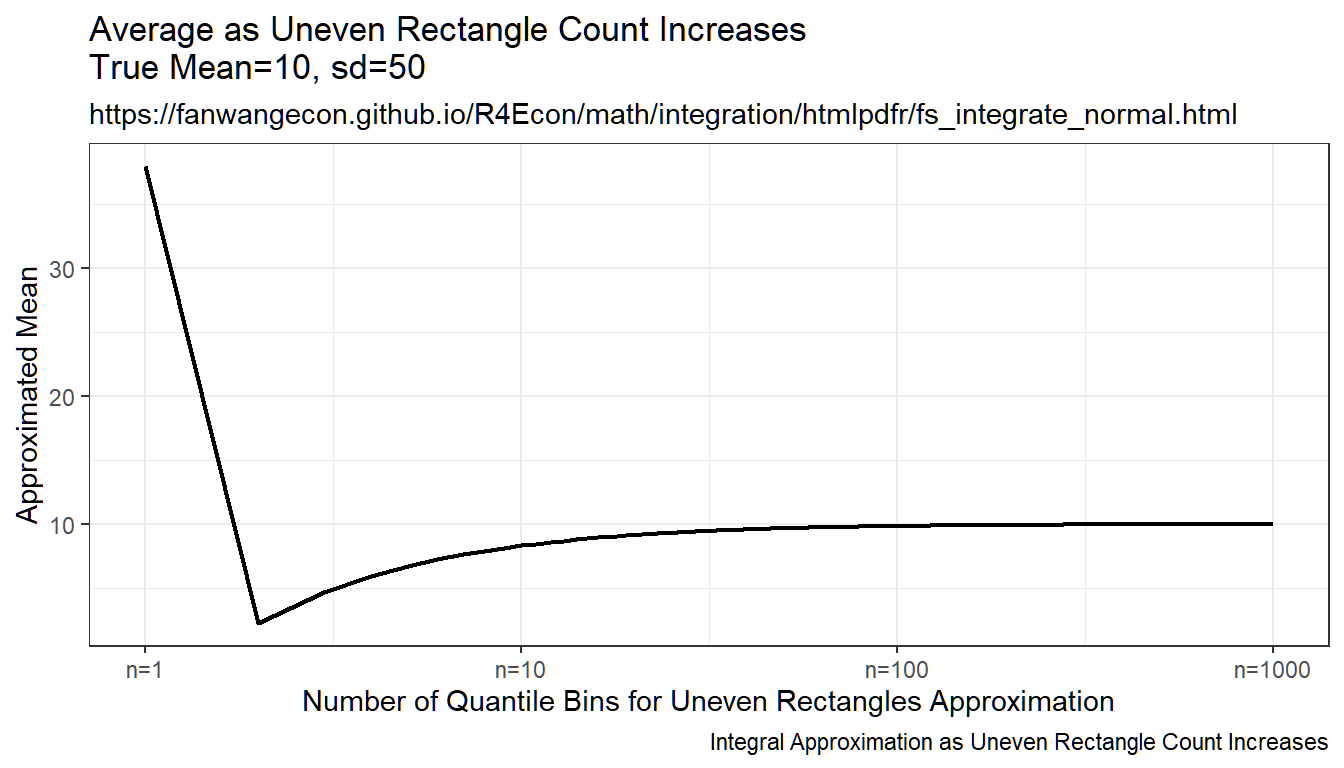
\includegraphics{Panel-Data-and-Optimization-with-R_files/figure-latex/unnamed-chunk-165-1} \end{center}

  \bibliography{book.bib,packages.bib}

\end{document}
